\documentclass{styles/tthesis}
\usepackage{cite}

\newcommand{\dspic}{dsPIC$^{\text{\textregistered}}$ DSC}
\newcommand{\dcbus}{DC-BUS\texttrademark }

\newif\ifwithqrcode
% Imposta a true per la versione con QR code,
% a false per la versione senza QR code.
\withqrcodetrue

% change the reference to the desired frontpage
\renewcommand{\frontpagefile}{frontpages/frontpage-ai4st.inc}

\title{Comprehensive assessment of MNCA for modelling complex biological systems}
\author{Luigi Daddario}
\renewcommand{\regnumber}{908294}
\graduation{Master's Degree in Artificial Intelligence for Science and Technology}
\academicyear{2024/2025}
\supervisor{
Prof. Paolo Napoletano \\
Co-supervisor: \\
Alex Graudenzi \\
}

%-------------------------------------------------------------------
\begin{document}
%-------------------------------------------------------------------

%-------------------------------------------------------------------
% Frontpage
%-------------------------------------------------------------------

% All "variable" data in the frontpage are set using the above commands.
\printfrontpage

%-------------------------------------------------------------------
% Abstract
%-------------------------------------------------------------------

\chapter*{Abstract}

This thesis investigated Mixture Neural Cellular Automata (MNCA) for modelling tissue-like dynamics, with emphasis on whether extending the spatial neighbourhood size (\(NB\)) improves learning and long-horizon stability. Neural cellular automata learn local update rules from data; the amount of spatial context each cell receives is controlled by \(NB\). We asked how this choice affects the ability of MNCA to maintain coherent, biologically plausible behaviour when run autonomously over long rollouts.

We used a synthetic tissue-growth simulator to generate supervised trajectories that reproduce key aspects of tissue-like dynamics. Using these data, we trained MNCA and Stochastic Mixture NCA across multiple neighbourhood sizes and evaluated them under free rollout at several horizons. In a controlled neighbourhood sweep (Step~3) we varied only \(NB\); its effect on performance was assessed with non-parametric tests. We also evaluated Stochastic Mixture NCA on the synthetic cell-imaging benchmark BBBC031, where the model grows a mask from seed points toward a ground-truth target. On BBBC031, we trained MNCA on this benchmark. Given the exploratory nature of the experiment and the objective of analysing learning dynamics rather than generalisation, models were evaluated in-sample (each model on the same image it was trained on); larger neighbourhoods were harder to optimise unless learning rate and training length were adapted.

The results show that neighbourhood size is a key determinant of performance. Beyond a minimal local context, performance did not seem to improve monotonically with \(NB\): different neighbourhood sizes induced different trade-offs between global distributional accuracy and spatial structure, and the ``best'' setting depended on which metric was prioritised and on the rollout horizon used for evaluation. In long-horizon free rollout (curriculum evaluation at 100 and 500 steps), the stochastic variant was more reliable and tended to outperform the deterministic one on distributional metrics (e.g., categorical MMD around 0.04 to 0.05 at \(NB=5\)), while the deterministic model could remain competitive on spatial metrics at intermediate neighbourhoods. The evaluation protocol strongly influenced interpretability: alignment between training and free-rollout evaluation and the use of multiple rollout horizons were necessary to observe these effects, which could otherwise be masked by exposure bias.

In conclusion, the experiments show that MNCA can reproduce tissue-like dynamics in a controlled synthetic setting, but that neighbourhood size and stochasticity change the long-horizon regime: once \(NB\ge2\), performance is non-monotonic and metric-dependent, and stable free-rollout behaviour requires evaluating at multiple horizons and keeping the train--evaluation protocol aligned.

\thispagestyle{empty}
\mbox{}
\newpage


%-------------------------------------------------------------------
% Dedication / Epigraph
%-------------------------------------------------------------------
\chapter*{\mbox{}}
\begin{flushright}
\thispagestyle{empty}
\null\vspace*{\stretch{1}}
{\it ``Nothing is as practical as a good theory.''}

\vspace{10pt}
--- Kurt Lewin
\vspace{\stretch{2}}\null
\end{flushright}
\newpage

%-------------------------------------------------------------------
% Acknowledgments
%-------------------------------------------------------------------
\chapter*{Acknowledgments}

I thank my supervisor, Prof.\ Paolo Napoletano, and my co-supervisor, Alex Graudenzi, for their guidance and for the opportunity to work on this project.

\ifwithqrcode
  \begin{center}
  \vspace{1cm}
  \qrcode[hyperlink,height=3cm]{https://v0-thesis-page-with-ai.vercel.app/}
  \end{center}
\fi

\thispagestyle{empty}
\mbox{}
\newpage


%-------------------------------------------------------------------
% Indexes
%-------------------------------------------------------------------

\tableofcontents
\listoffigures
\listoftables

\mainmatter

%-------------------------------------------------------------------
\chapter{Introduction}
\label{c:intro}
%-------------------------------------------------------------------

%-------------------------------------------------------------------
\section{Context and motivation}
\label{sec:intro:context}
%-------------------------------------------------------------------

Tissues and other multicellular structures arise from the repeated application of local rules: cells divide, differentiate, migrate, and respond to signals from their immediate neighbourhood.
No single cell holds a global blueprint; instead, large-scale morphology and function emerge from many spatially distributed, short-range interactions.
A central question in developmental and systems biology is how such local rules give rise to stable patterns and robust growth. This has led to a long tradition of computational models that emphasise locality and discreteness \cite{ca_vonneumann1966}.

This thesis focuses on a class of such models: neural cellular automata \cite{nca_mordvintsev2020} trained to imitate tissue-like dynamics.
We ask whether these models can both reproduce short-term transitions from data and maintain coherent, biologically plausible behaviour when run autonomously over long horizons.
In that setting, the choice of how much spatial context each cell uses (the size of its ``neighbourhood'') becomes a key design factor.
We therefore assess Mixture Neural Cellular Automata (MNCA) \cite{mnca_milite2025} in a controlled tissue-growth scenario and ask whether enlarging the neighbourhood improves learning and long-horizon stability.

From a data point of view, the \emph{input} to the MNCA is a discrete grid representing a tissue state at a given time (cell types on a lattice), and the \emph{output} is the next grid obtained by applying the learned local rule everywhere.
Training uses pairs (or short windows) of consecutive tissue states from a simulator as supervision; deployment consists of iterating the learned rule from an initial condition to generate a full trajectory.
The central question is therefore whether one can learn a local update rule that, when repeatedly applied to realistic initial conditions, reproduces the distribution of tissue-like histories observed in the data.

%-------------------------------------------------------------------
\section{Why cellular automata and neural cellular automata}
\label{sec:intro:why_ca}
%-------------------------------------------------------------------

Cellular automata (CA) \cite{ca_vonneumann1966} provide one of the simplest frameworks for studying emergence from local rules: a discrete grid of cells is updated in parallel according to a fixed rule that depends only on each cell's state and that of its neighbors.
They have been used for decades to model physical, chemical, and biological phenomena, from pattern formation to morphogenesis, without requiring continuous equations or global coordination.
This makes them a natural fit when the phenomenon of interest is inherently local and when interpretability and parsimony matter.

Neural cellular automata (NCA) \cite{nca_mordvintsev2020} retain the same spatial structure and locality but replace the hand-crafted update rule with a learned one, typically a small neural network that takes the local neighbourhood as input.
Thus, one keeps the inductive bias of ``local rules only'' while gaining the flexibility to discover dynamics from data.
Mixture variants \cite{mnca_milite2025} go a step further by combining several learned rules with stochasticity, which is well suited to biological systems where variability and multiple cell behaviors are the norm.

An alternative would be to model the same dynamics with generic deep learning: for example, a convolutional or recurrent network that maps full grid states across time.
Such models can be powerful, but they do not enforce locality by design; the effective receptive field and the way information propagates are less transparent, and long-horizon rollout often suffers from drift or instability.
By contrast, CA and NCA explicitly encode the prior that only nearby cells influence each other, which aligns with the biological picture and can improve generalization and stability when the training signal is limited or noisy.
In short, we treat cellular automata and neural cellular automata as a structured, spatially grounded class of models within machine learning. This class trades some flexibility for interpretability, parsimony, and a bias that matches the problem.
From a computational perspective, MNCA can be seen as a learnable \emph{spatio-temporal simulator}: a data scientist provides trajectories of tissue states as input, and the model learns a local transition rule that can be rolled out to produce new trajectories.
The aim in this thesis is to understand when such a model can be trusted to generate long-horizon behaviour that remains close to biologically motivated ground truth, and how the neighbourhood size influences this capability.

%-------------------------------------------------------------------
\section{Objectives of the thesis}
\label{sec:intro:objectives}
%-------------------------------------------------------------------

The main objective of this thesis is to evaluate Mixture Neural Cellular Automata in a tissue-growth setting and to see whether using a larger spatial neighbourhood helps them learn better and keep plausible dynamics over long rollouts.
To that end, we design a sequence of experiments that progressively refine the training setup and the evaluation protocol.
We compare multiple neighbourhood sizes using both qualitative inspection of rollouts and quantitative metrics, and we discuss how the choice of neighbourhood interacts with other factors such as curriculum design and evaluation horizon.
A secondary aim is to provide a reproducible experimental pipeline and a clear reporting of results, so that the findings can be extended or challenged in future work.

%-------------------------------------------------------------------
\section{Organization of the document}
\label{sec:intro:organization}
%-------------------------------------------------------------------

\Cref{c:sota} reviews the state of the art on cellular automata, neural cellular automata, and mixture-based extensions.
\Cref{c:tools} describes the software stack and the organization of the codebase used for the experiments.
\Cref{c:implementation} details the implementation of the experiments: the synthetic biological simulator, the training and evaluation pipeline, and the design of the neighbourhood-size sweep.
\Cref{c:results} summarizes the main findings and their implications.
\Cref{c:conc} draws conclusions and outlines possible directions for future work.

%-------------------------------------------------------------------
\chapter{State of the Art}
\label{c:sota}
%-------------------------------------------------------------------

%-------------------------------------------------------------------
\section{Context, data, and the case for structured spatial models}
\label{sec:sota:context}
%-------------------------------------------------------------------

Modelling spatially organised biological systems has a long tradition in mathematical and computational biology. The spatial arrangement of cells and the local signals they exchange strongly affect form and function. For example, morphogen gradients govern cell fate during development~\cite{rogers2011morphogen}; stem-cell identity and niche behaviour depend on spatial context; and both cancer invasion and tissue regeneration are driven by local cell-cell and cell-environment interactions in spatially structured tissues~\cite{noble2022spatial,seferbekova2023spatial}. So any computational model that aims to capture these phenomena must represent space explicitly. It must also respect the constraint that no single agent has access to global state: each cell may use only information from its immediate neighbourhood.
Classical approaches fall into two broad categories:
\begin{enumerate}
  \item \emph{Continuum models}, which use partial differential equations (reaction-diffusion, mechanochemical formulations).
  \item \emph{Discrete agent-based models}, in which each cell obeys rules that depend on local context.
\end{enumerate}
The first type is tractable in simple geometries but scales poorly to highly heterogeneous, discrete cell populations. The second is flexible and widely used in tissue and cancer modelling, but the rules are usually hand-tuned or fitted via simulation-based inference (e.g.\ approximate Bayesian computation~\cite{beaumont2002abc,sisson2018abc}). Learning such rules directly from high-dimensional observational data remains challenging. A central question in recent work is therefore how to combine spatial, local interaction with the ability to \emph{learn} dynamics from data using gradient-based optimisation \cite{mnca_milite2025}.

The data used to train or validate such models are diverse. In developmental biology and morphogenesis, target data may be static patterns (e.g.\ a desired shape or cell-type map) or temporal sequences of spatial configurations from time-lapse imaging or lineage tracing. In tissue and cancer modelling, researchers often use high-throughput microscopy, spatial transcriptomics, and synthetic data from stochastic simulators (e.g.\ stem-cell-driven growth and differentiation on a grid). In all cases, observations are high-dimensional (many cells, time points, or channels), and the underlying transition rules are unknown or only partly known. The goal is not only to fit the data but to obtain a \emph{mechanistic}, generative representation. Such a model can be run from new initial conditions, examined (e.g.\ to see which local rule applies where), and potentially steered by changing rules or initial state. This pushes the goal beyond pure prediction toward interpretable, generative spatial dynamics \cite{mnca_milite2025,nca_mordvintsev2020}.

An alternative is to use generic deep learning: for instance, convolutional or recurrent networks that map the current grid state (or a sequence of states) to the next state or to a target output. Such architectures have been used successfully for image-to-image prediction and video forecasting. However, they do not enforce locality by design. The effective receptive field of a deep convolutional network can span the entire grid, and how information propagates in space and time is encoded implicitly in the weights. There is no direct link to the biological assumption that cells communicate only with neighbours. In practice, long-horizon rollouts from these models often drift, diverge, or become unstable, especially when training data are limited or when the task requires extrapolation beyond the training distribution. Also, the learned dynamics are hard to interpret: one cannot easily extract a local rule or see which cells influence which. By contrast, cellular automata and their neural extensions assume that the next state of a cell depends only on a bounded neighbourhood. This bias restricts the hypothesis space, can improve sample efficiency when data are scarce, and yields models that match the mechanistic, agent-based view of biology used in much of the spatial modelling literature. The trade-off is less expressive power in exchange for interpretability, stability under rollout, and a parameterisation that fits the domain. The rest of this chapter surveys the literature along this line, from classical CA to neural and mixture-based CA, and places the model used in this thesis in a clear methodological and applied context.

%-------------------------------------------------------------------
\section{Cellular Automata}
\label{sec:sota:ca}
%-------------------------------------------------------------------

Cellular automata (CA) have been studied since the pioneering work of von Neumann on self-reproducing automata \cite{ca_vonneumann1966} and have since become a canonical framework for studying emergence from local rules; for a modern treatment see \cite{ca_hawkins2024}. A CA consists of a discrete grid of cells, each endowed with a state drawn from a finite (or, in continuous variants, real-valued) set. Time advances in discrete steps; at each step, every cell is updated according to a fixed rule that depends only on its own state and the states of the cells in a small neighbourhood. There is no central controller: the next configuration is determined solely by applying the same local rule everywhere in parallel. This formulation captures the essence of decentralised, spatially local computation and has been applied across physics, ecology, and biology; optimisation of CA rules via evolutionary curriculum strategies has also been explored \cite{ca_antal2021}.

Formally, let \(\mathcal{L}\) denote the set of cell positions (e.g.\ a finite or infinite subset of \(\mathbb{Z}^2\)), and \(\mathcal{S}\) the set of possible cell states. The neighbourhood of a cell at \((i,j)\) is a set \(\mathcal{N}(i,j) \subseteq \mathcal{L}\) of nearby positions (e.g.\ those within Chebyshev distance \(r\) for some radius \(r\)). The global state at time \(t\) is a function \(x_t : \mathcal{L} \to \mathcal{S}\). The update rule is a function \(\phi\) that maps the state of a cell and its neighbourhood to a new state:
\begin{equation}
x_{t+1}(i,j) = \phi\bigl( x_t(i,j), \, \{ x_t(i',j') : (i',j') \in \mathcal{N}(i,j) \} \bigr).
\end{equation}
The dynamics are fully specified by \(\phi\) and the initial condition \(x_0\). Despite this simplicity, CAs are known to exhibit a wide range of behaviours (from static or periodic patterns to chaos, self-replication, and universal computation) and have been the subject of extensive theoretical and applied work. In the biological context, the emphasis on locality and discreteness aligns with the view that cells interact primarily with nearby cells and that developmental and tissue-level dynamics can be approximated by discrete-time updates. CAs have accordingly been used as tools for simulating growth, pattern formation, and morphogenesis in the literature \cite{ca_vonneumann1966}. See \cref{fig:sota:ca_example} for an illustration.

\begin{figure}[t]
  \centering
  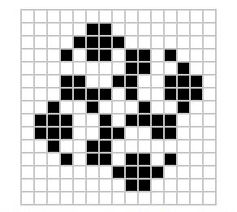
\includegraphics[width=0.62\textwidth]{figs/sota_ca_example}
  \caption{Example of a cellular automaton. \textbf{Legend:} discrete grid; each cell updated by a local rule~\cite{ca_vonneumann1966}.}
  \label{fig:sota:ca_example}
\end{figure}

The main limitation here is that the rule \(\phi\) is fixed and hand-crafted. Inverse design (finding a \(\phi\) that produces a desired global behaviour, e.g.\ a specific shape or regenerative response, from a simple seed) is difficult. Reverse-engineering such rules for biologically plausible outcomes is still an open problem. This has led to work where the update rule is \emph{learned} from data instead of being set in advance, i.e.\ to the neural cellular automata discussed in the next section.

%-------------------------------------------------------------------
\section{Neural Cellular Automata}
\label{sec:sota:nca}
%-------------------------------------------------------------------

Gilpin showed that CA update rules can be expressed as convolutional neural networks \cite{ca_gilpin2019}. Mordvintsev et al.\ then showed that such rules can be \emph{learned} from data via gradient-based optimisation, leading to what is now called Neural Cellular Automata (NCA) \cite{nca_mordvintsev2020}. NCAs keep the spatial structure and locality of classical CAs but replace the hand-crafted rule \(\phi\) with a function implemented by a small neural network. The same network is applied at every cell; only the local perception (and, in some extensions, a small amount of global conditioning) varies across the grid. Formally, NCAs replace \(\phi\) in the classical CA update with a learned map \(f_\theta\) that takes a local view of the grid and outputs an update (typically an increment) to the cell state.

A common formulation is
\begin{equation}
x_{t+1} = x_t + f_\theta\bigl( \mathcal{P}(x_t) \bigr),
\end{equation}
where \(\mathcal{P}(x_t)\) denotes a \emph{perception} step that, for each cell, aggregates information from a neighbourhood (e.g.\ the cell's own state plus gradient-like features in the horizontal and vertical directions, as in the Growing NCA model below). The network \(f_\theta\) is typically a shallow stack of \(1\times 1\) convolutions and nonlinearities, so that it operates in a local fashion and can be applied in one pass over the grid. Training is usually performed by minimising a loss between the state produced after a number of steps and a target (e.g.\ an image or a temporal trajectory), using backpropagation through time (BPTT)~\cite{werbos1990backpropagation,goodfellow2016deep}. Subsequent work has extended NCAs to texture synthesis, 3D morphogenesis, and classification tasks, and has explored variants with attention mechanisms, graph-based neighbourhoods, and Hamiltonian-inspired conservative dynamics~\cite{hnn_ca_greydanus2021}; the core idea of a single, learned local rule applied everywhere remains central \cite{nca_mordvintsev2020}, and recent work has examined both interpretability of the learned rules and their application to biological systems \cite{nca_bodnar2022,nca_randall2023}.

This shift from fixed to learned rules has several consequences that are relevant to the present thesis. First, NCAs can be trained to reproduce complex target dynamics (morphogenesis, texture synthesis, regeneration) without explicitly programming the transition rule. Second, the model remains interpretable in the sense that behaviour is driven exclusively by local updates. Third, the framework is differentiable end-to-end, so objectives can be defined at the level of global outcomes (e.g.\ match a target pattern) and the local rule can be optimised accordingly. For these reasons, NCAs have been adopted as a natural tool for modelling biological and self-organising systems where the goal is to learn growth and patterning from data rather than to postulate a specific \(\phi\) \cite{nca_mordvintsev2020}. \Cref{fig:sota:nca_schema} illustrates the generic NCA step.

\begin{figure}[t]
  \centering
  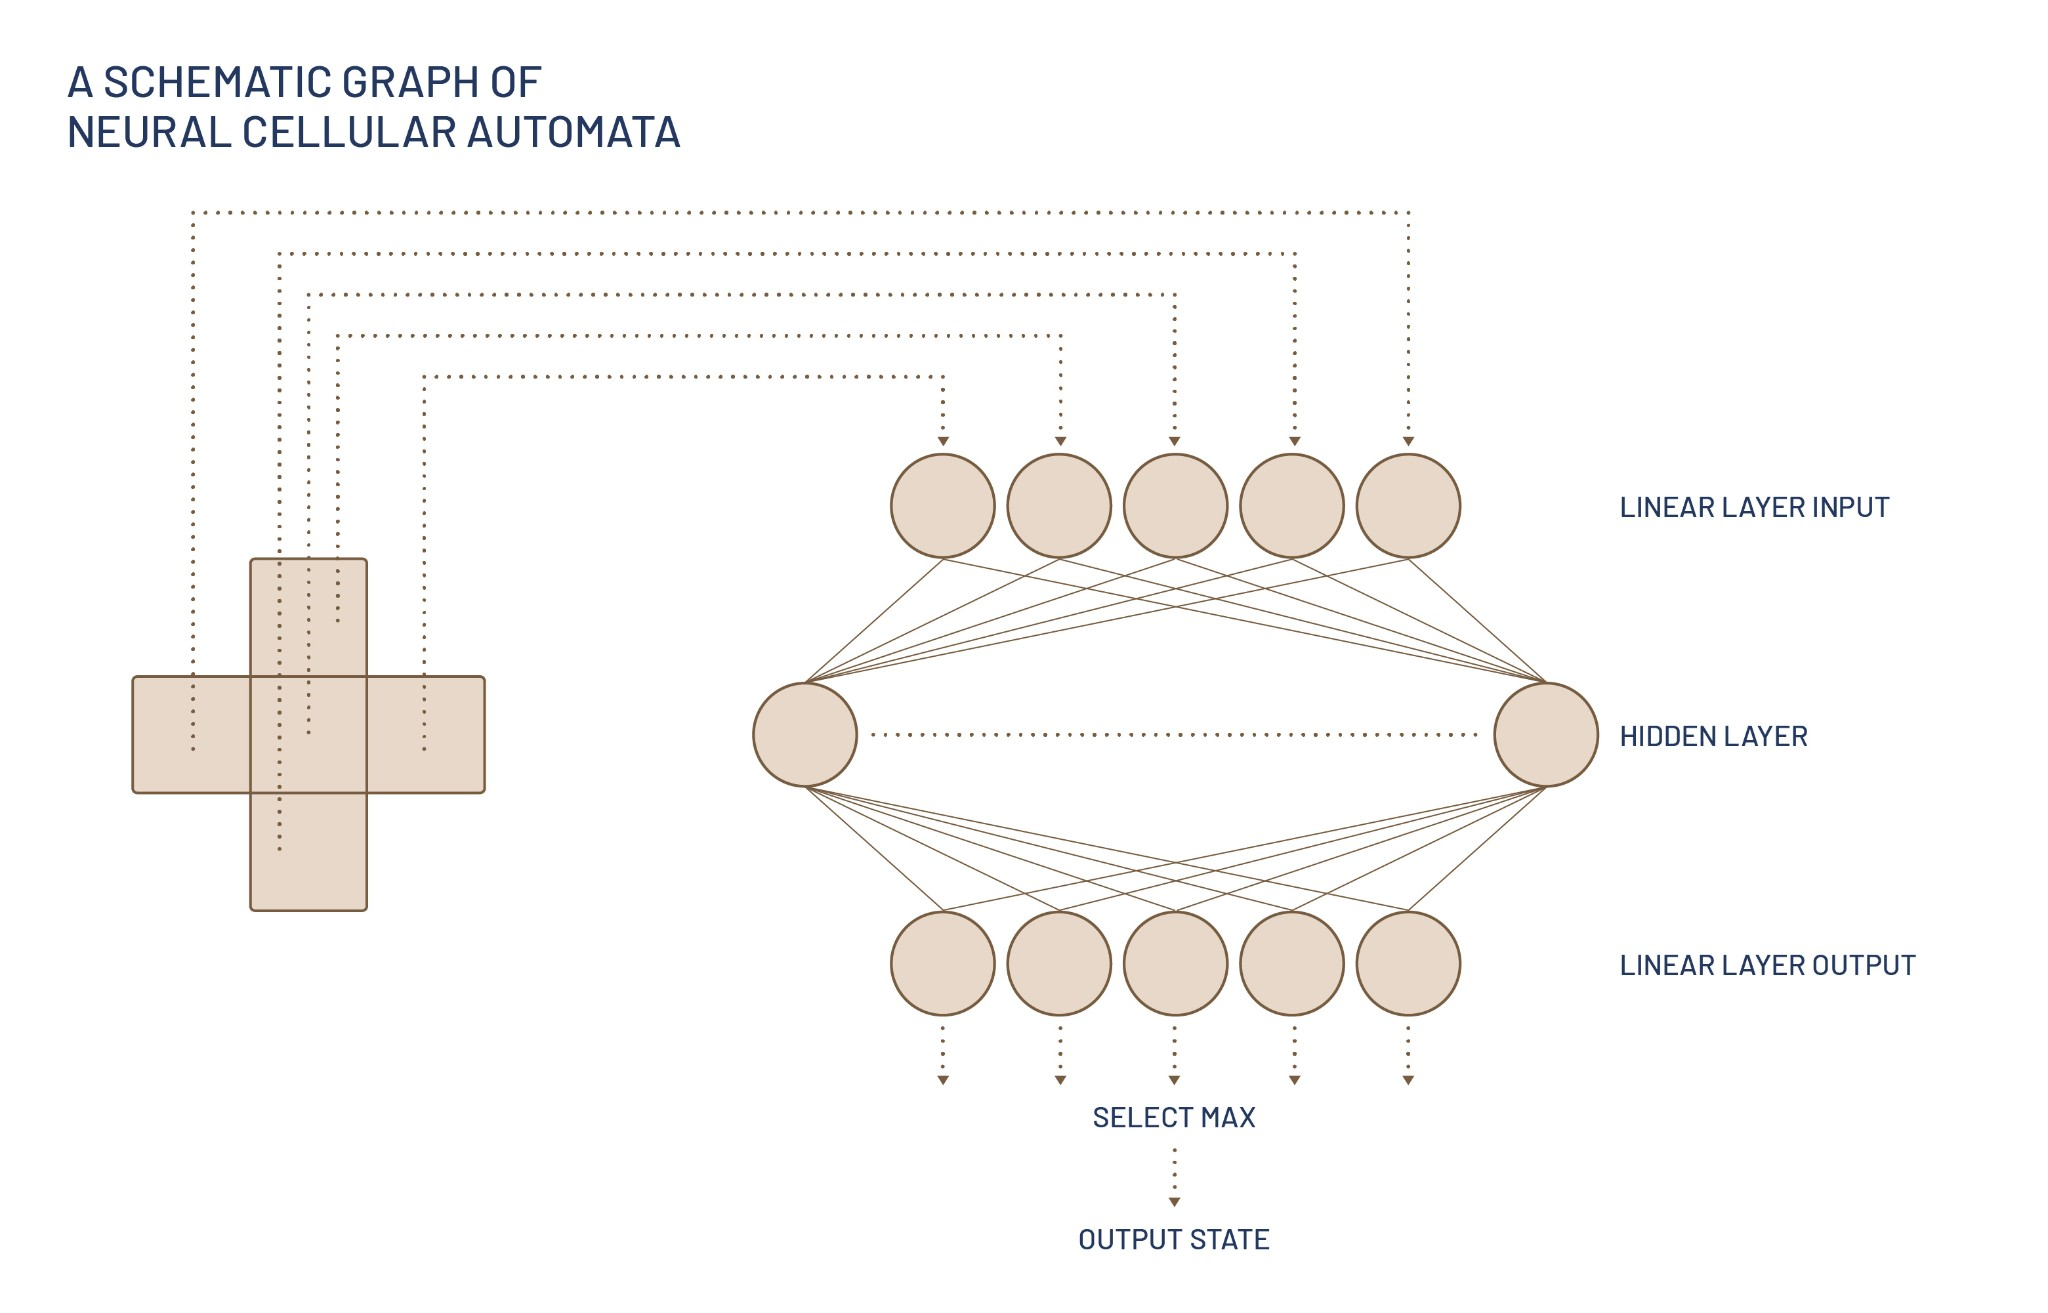
\includegraphics[width=0.72\textwidth]{figs/sota_nca_schema}
  \caption{Single NCA update step. \textbf{Legend:} perception (state and gradients) \(\rightarrow\) neural network \(\rightarrow\) state increment (applied residually). Adapted from Mordvintsev et al.~\cite{nca_mordvintsev2020}.}
  \label{fig:sota:nca_schema}
\end{figure}

%-------------------------------------------------------------------
\section{Growing Neural Cellular Automata}
\label{sec:sota:growing}
%-------------------------------------------------------------------

Mordvintsev et al.\ introduced \emph{Growing Neural Cellular Automata} in a setting that focuses explicitly on morphogenesis: the NCA is trained to grow a predefined multicellular pattern on a 2D grid from a single seed cell \cite{nca_mordvintsev2020}. This setting has since served as a reference benchmark and as a bridge between abstract NCA and biologically inspired notions of growth, stability, and regeneration.

\subsection{Cell state and perception}

Each cell is represented by a vector of 16 real values. The first three channels are RGB (the visible phenotype); the fourth is an alpha channel used to distinguish ``living'' cells (alpha \(> 0.1\)) from empty ones. The remaining channels are latent and used by the rule for internal signalling. Cells with no living neighbour in their \(3\times 3\) neighbourhood have their state set to zero at each step, so that only the pattern and its immediate frontier participate in the dynamics.

Perception is implemented by augmenting the cell state with local gradient information. Convolving the grid with Sobel filters~\cite{sobel1968isotropic} in the \(x\) and \(y\) directions yields, for each channel, estimates of \(\partial/\partial x\) and \(\partial/\partial y\)~\cite{szeliski2022computer}. The perception vector for a cell is the concatenation of its state, the gradients in \(x\), and the gradients in \(y\), giving a \(16 \times 3 = 48\)-dimensional input per cell. This design reflects the idea that cells in real morphogenesis often rely on chemical or electrical gradients to coordinate; the Sobel filters provide a fixed, differentiable way to sense direction and rate of change.

\subsection{Update rule and stochasticity}

The update rule is a small fully connected (or equivalently \(1\times 1\) convolutional) network that maps the 48-dimensional perception to a 16-dimensional state increment. The final layer is initialised to zero so that the initial behaviour is close to ``do nothing'', and no ReLU is applied to the output so that updates can be positive or negative. The state is updated in a residual fashion: \(x_{t+1} = x_t + \Delta x_t\). \Cref{fig:sota:growing_update} summarises one full update step (perception, update, stochastic mask, alive masking).

To relax the assumption of a global synchronous clock, the model applies a random per-cell mask to the update: with probability 0.5 (during training), the update at a cell is zeroed. Thus cells effectively update at random times, which can improve robustness and is closer to asynchronous biological update.

\begin{figure}[t]
  \centering
  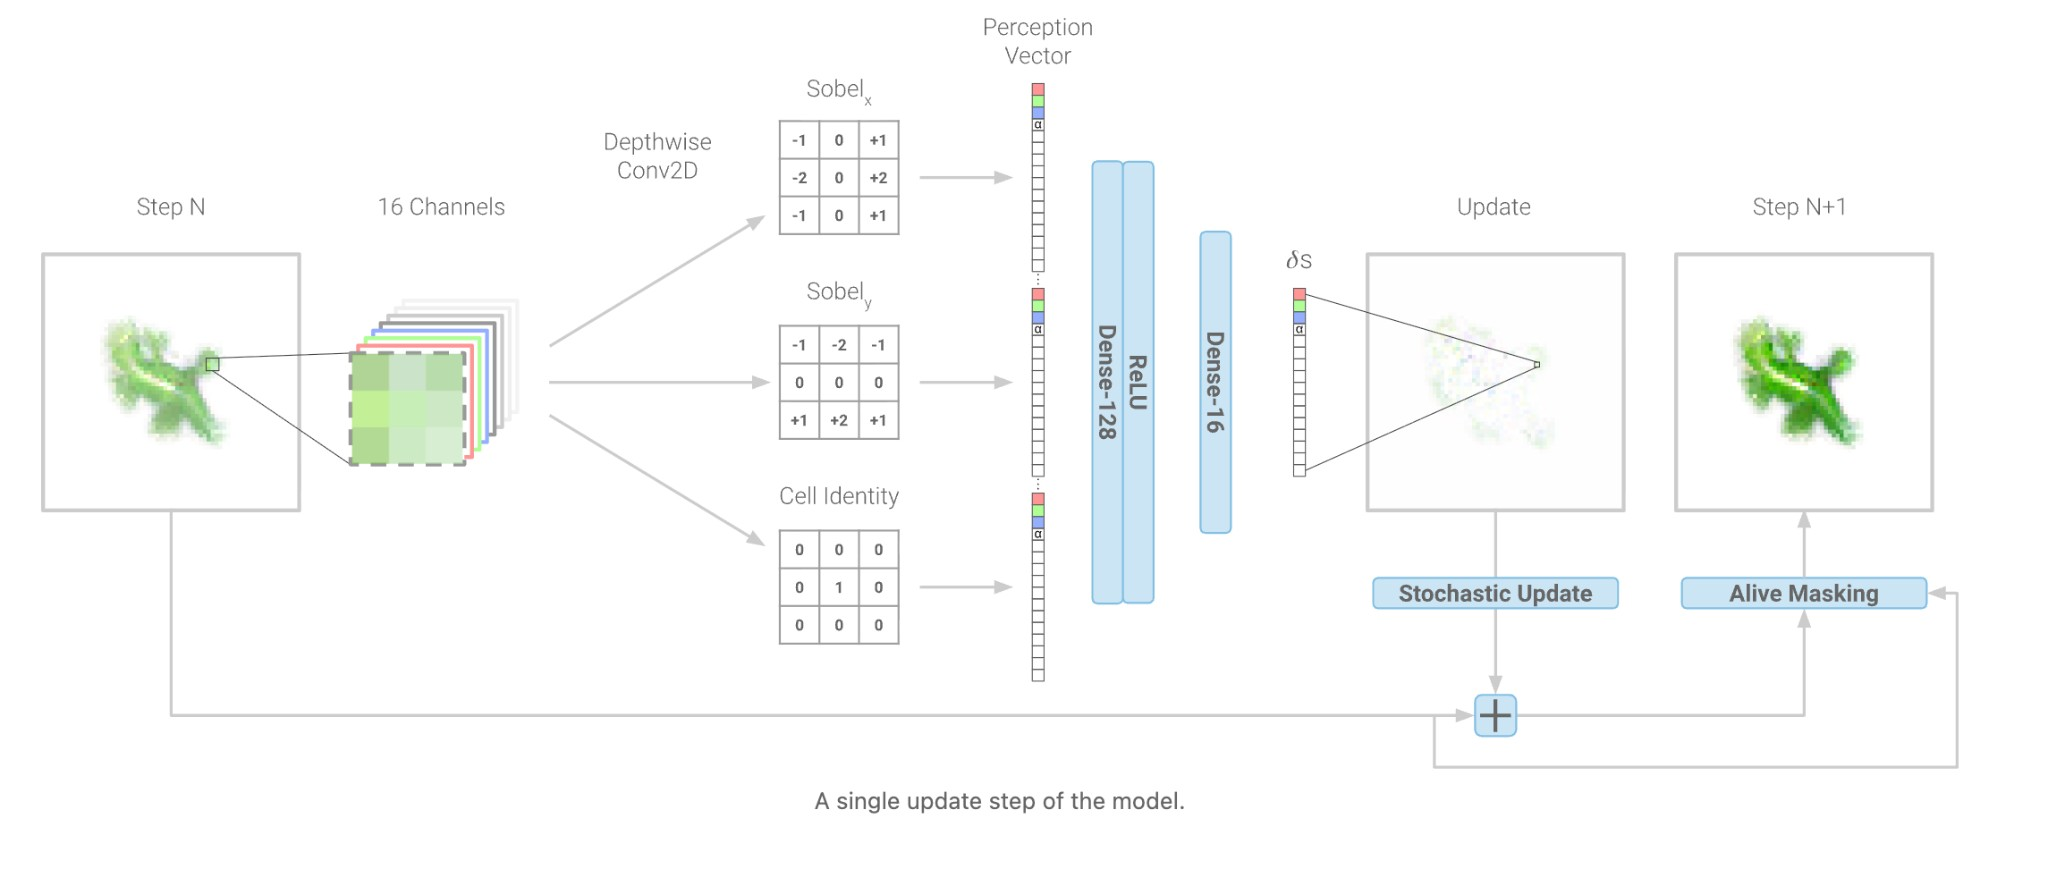
\includegraphics[width=0.76\textwidth]{figs/sota_growing_update}
  \caption{One update step of the Growing NCA. \textbf{Legend:} perception (state + gradient channels) \(\rightarrow\) update network \(\rightarrow\) stochastic mask \(\rightarrow\) alive masking. Adapted from Mordvintsev et al.~\cite{nca_mordvintsev2020}.}
  \label{fig:sota:growing_update}
\end{figure}

\subsection{Training for growth, persistence, and regeneration}

Training proceeds in three phases \cite{nca_mordvintsev2020}. In the first, the CA is trained to reach a target pattern from a single seed after a random number of steps in a fixed range; the loss is pixel-wise L2 between the final state and the target. This yields growth but often unstable long-term behaviour (patterns may explode or decay). In the second phase, a \emph{sample pool} of states is maintained: at each training step, a batch is sampled from the pool, the highest-loss sample is replaced by the seed, and the model is run on the batch; the resulting states are written back into the pool. The dynamics are thus trained not only to grow from the seed but also to persist and to correct from states that are already close to or far from the target, encouraging the target to become an attractor in the dynamical-systems sense (a configuration toward which trajectories converge and remain). In the third phase, a subset of the pool samples is \emph{damaged} (e.g.\ by zeroing a random circular region) before iteration, so that the model must learn to regenerate. Models trained with this damage regime exhibit substantially stronger regenerative behaviour than those trained only for growth or persistence \cite{nca_mordvintsev2020}. \Cref{fig:sota:growing_training_steps} shows the evolution of a pattern during training; \cref{fig:sota:growing_pool} and \cref{fig:sota:growing_regeneration} illustrate pool-based training and regeneration.

\begin{figure}[t]
  \centering
  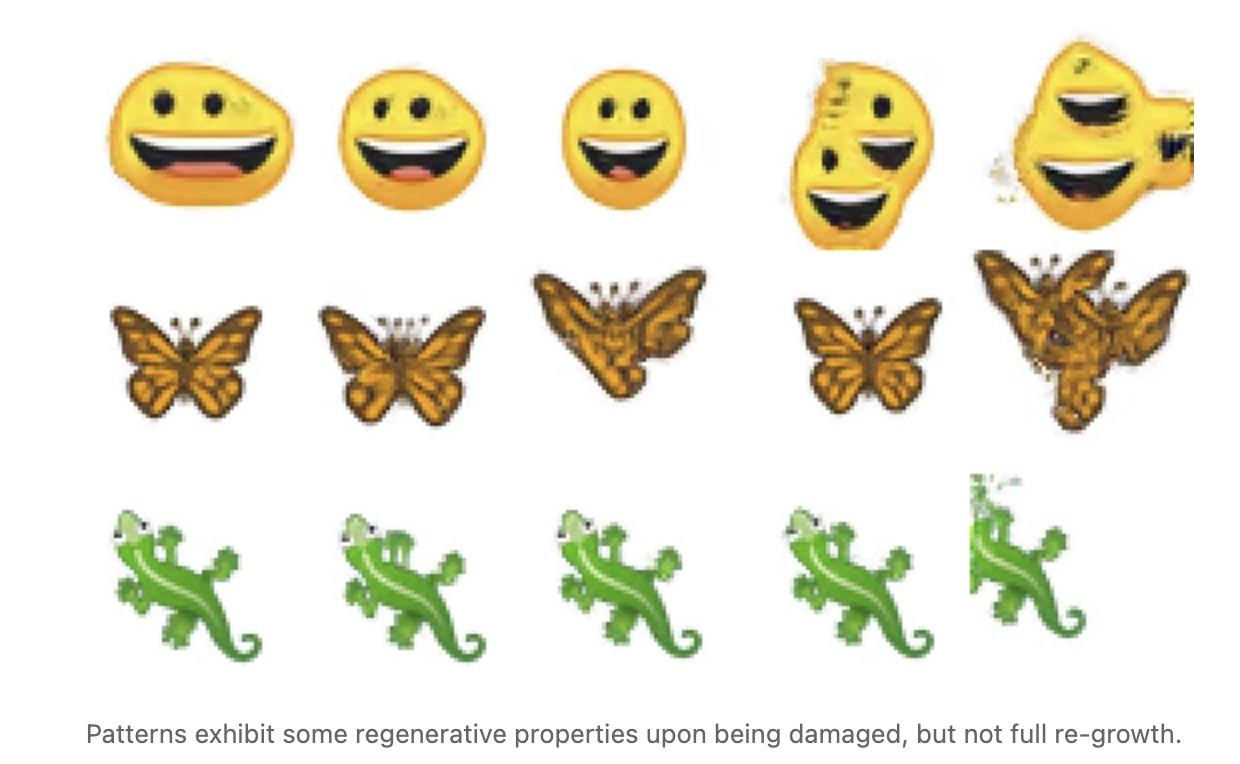
\includegraphics[width=0.72\textwidth]{figs/sota_growing_training_steps}
  \caption{CA behaviour at training steps 100, 500, 1000, 4000. \textbf{Legend:} columns = training step; pattern evolves from initial seed toward target. Adapted from Mordvintsev et al.~\cite{nca_mordvintsev2020}.}
  \label{fig:sota:growing_training_steps}
\end{figure}

\begin{figure}[t]
  \centering
  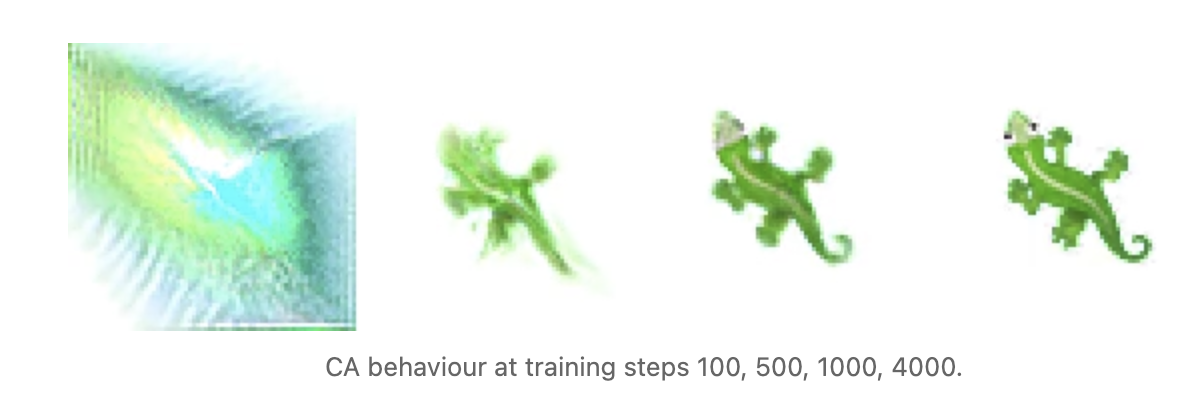
\includegraphics[width=0.72\textwidth]{figs/sota_growing_pool}
  \caption{Sample-pool training. \textbf{Legend:} random sample of patterns in the pool during training. Adapted from Mordvintsev et al.~\cite{nca_mordvintsev2020}.}
  \label{fig:sota:growing_pool}
\end{figure}

\begin{figure}[t]
  \centering
  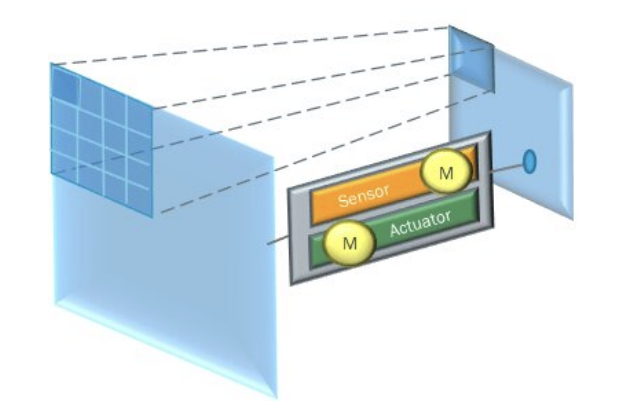
\includegraphics[width=0.72\textwidth]{figs/sota_growing_regeneration}
  \caption{Regeneration. \textbf{Legend:} pattern damaged then iterated; extent of recovery shown. Adapted from Mordvintsev et al.~\cite{nca_mordvintsev2020}.}
  \label{fig:sota:growing_regeneration}
\end{figure}

This progression (growth, persistence, regeneration) demonstrates that a single local rule, learned with appropriate objectives and data diversity, can capture morphogenetic and homeostatic behaviour. It also motivates the next step in the literature: the introduction of multiple rules and explicit stochasticity to better match the variability and heterogeneity of real biological systems.

%-------------------------------------------------------------------
\section{Limits of Standard NCA and the Role of Stochasticity}
\label{sec:sota:limits}
%-------------------------------------------------------------------

Standard NCA models, including the Growing NCA described above, are deterministic: given the same initial state and the same (possibly stochastic) update mask, the trajectory is uniquely determined. It is well established in the biological literature that real systems are inherently stochastic: gene expression, cell division, and differentiation are subject to molecular noise; genetically identical cells can follow different fates; and tissue-level outcomes emerge from the statistics of many such noisy, local events. Deterministic NCAs can at best produce a single ``average'' trajectory and do not naturally represent variability across runs or the possibility that different cells might follow different behavioural programmes.

Furthermore, in real morphogenesis and tissue maintenance, cells are not all executing the same programme: they differentiate into distinct types and adopt different roles. A single global update rule can encode complex behaviour through the hidden state, but it does not explicitly represent a \emph{mixture} of distinct local behaviours (e.g.\ one rule favouring proliferation at the border, another maintaining quiescence in the interior). These observations have motivated a line of work that extends the NCA framework to support multiple update rules and stochastic selection among them, so that both spatial heterogeneity (different rules in different regions) and variability across realisations can be captured. The Mixture of Neural Cellular Automata (MNCA) framework, reviewed in the next section, implements this extension \cite{mnca_milite2025}.

%-------------------------------------------------------------------
\section{Mixture of Neural Cellular Automata}
\label{sec:sota:mnca}
%-------------------------------------------------------------------

Milite et al.\ \cite{mnca_milite2025} introduced the Mixture of Neural Cellular Automata (MNCA), a framework that addresses two limitations of standard NCAs: their deterministic nature, which poorly matches the stochasticity of real biological systems (e.g.\ gene expression, cell differentiation, carcinogenesis), and the lack of an explicit representation of heterogeneous local behaviours. By combining mixture models with the NCA paradigm, MNCA allows each cell to be governed by one of \(K\) distinct neural update rules, with the choice made probabilistically from the current state. The authors further propose an extension with \emph{intrinsic noise}: a Gaussian latent vector fed into each rule so that even the same rule can produce stochastic updates, thereby capturing intra-cluster variability. The result is a stochastic, spatially heterogeneous dynamics that can be trained end-to-end and that offers interpretable rule assignments for post-hoc analysis \cite{mnca_milite2025}. MNCA constitutes the central model used in this thesis; all experiments reported in \cref{c:implementation} and \cref{c:results} are based on it.

\subsection{Formal definition and two variants}

Consider a grid of cells; let \(s^t_i \in \mathcal{S}\) denote the state of cell \(i\) at time \(t\) and \(\mathcal{N}(i)\) its neighbourhood. The authors define \(K\) neural transition functions \(\phi_k(\cdot; \theta_k)\), each mapping the local configuration (cell state and neighbours) to a state increment. A \emph{rule selector} is a neural network \(\pi(\cdot; \eta)\) that, given the current cell state (and optionally noise), outputs a \(K\)-dimensional probability vector over rules.

\paragraph{Mixture NCA (no intrinsic noise).} The rule index for cell \(i\) at time \(t\) is drawn from a Categorical distribution parametrised by \(\pi(s^t_i; \eta)\). Denoting by \(z \in \{1,\ldots,K\}\) the selected rule (one-hot encoded as \(z_k\)), the update is
\begin{equation}
z \sim \mathrm{Cat}\bigl(\pi(s^t_i; \eta)\bigr), \qquad
s^{t+1}_i = s^t_i + \sum_{k=1}^{K} z_k \, \phi_k\bigl(s^t_i, \{s^t_j : j \in \mathcal{N}(i)\}; \theta_k\bigr).
\end{equation}
Thus exactly one rule applies per cell per step; the Categorical is sampled so that the process is stochastic. To backpropagate through the discrete choice, the authors use the Gumbel-Softmax / Concrete trick~\cite{jang2017gumbel,maddison2017concrete,mnca_milite2025}.

\paragraph{MNCA with intrinsic noise.} Biological systems often exhibit variability even among cells that share the same ``type'' or context. To allow for intra-rule stochasticity, the update functions are given an extra input \(x_k \sim \mathcal{N}(0, I)\) sampled once per rule (or per cell and rule) and concatenated to the perception. The update becomes
\begin{equation}
z \sim \mathrm{Cat}\bigl(\pi(s^t_i; \eta)\bigr), \quad
x_k \sim \mathcal{N}(0, 1), \qquad
s^{t+1}_i = s^t_i + \sum_{k=1}^{K} z_k \, \phi_k\bigl(s^t_i, \{s^t_j : j \in \mathcal{N}(i)\}, x_k; \theta_k\bigr).
\end{equation}
The noise \(x_k\) is an internal source of randomness that the network can use to implement stochastic behaviour within each rule (e.g.\ random timing of division or differentiation). In the paper's experiments, both variants are evaluated; the one with intrinsic noise often yields better robustness and more realistic tissue statistics \cite{mnca_milite2025}.

\subsection{Architecture and implementation}

The paper keeps a simple, consistent architecture across tasks. Perception is the same as in many NCAs: the state is concatenated with its spatial gradients in \(x\) and \(y\) obtained via Sobel filters, i.e.\ \(\mathcal{P}(s) = \mathrm{cat}(s, \nabla_x s, \nabla_y s)\). Each rule \(\phi_k\) is implemented as two \(1\times 1\) convolutional layers: a hidden layer with ReLU on the perceived input (and, in the noisy variant, concatenated with \(x_k\)), then a linear layer that outputs the state increment. The rule selector \(\pi\) is a network of the same type but takes only the \emph{current cell state} \(s^t_i\) as input (not the full perception), so that the assignment depends on the cell's own state rather than on neighbour states. Training uses the mean squared error between the predicted and target state; optimisation is performed with Adam~\cite{kingma2014adam} and a multi-step learning-rate schedule, as is standard in deep learning~\cite{goodfellow2016deep}. Depending on the task, the update is applied as a residual (\(s^{t+1}_i = s^t_i + \Delta s\)) or the state is replaced entirely. Key hyperparameters (number of channels, number of rules \(K\), hidden dimension, residual or not) are reported per experiment: for example, the tissue-growth setup uses 6 channels, 5 rules, hidden dimension 128, and no residual update \cite{mnca_milite2025}. \Cref{fig:sota:mnca_schema} corresponds to Figure~1 in the paper, which summarises the full pipeline: spatial filters, central cell and neighbours, rule selector (MLP) yielding rule probabilities, and the selected NCA with optional noise injection.

\begin{figure}[t]
  \centering
  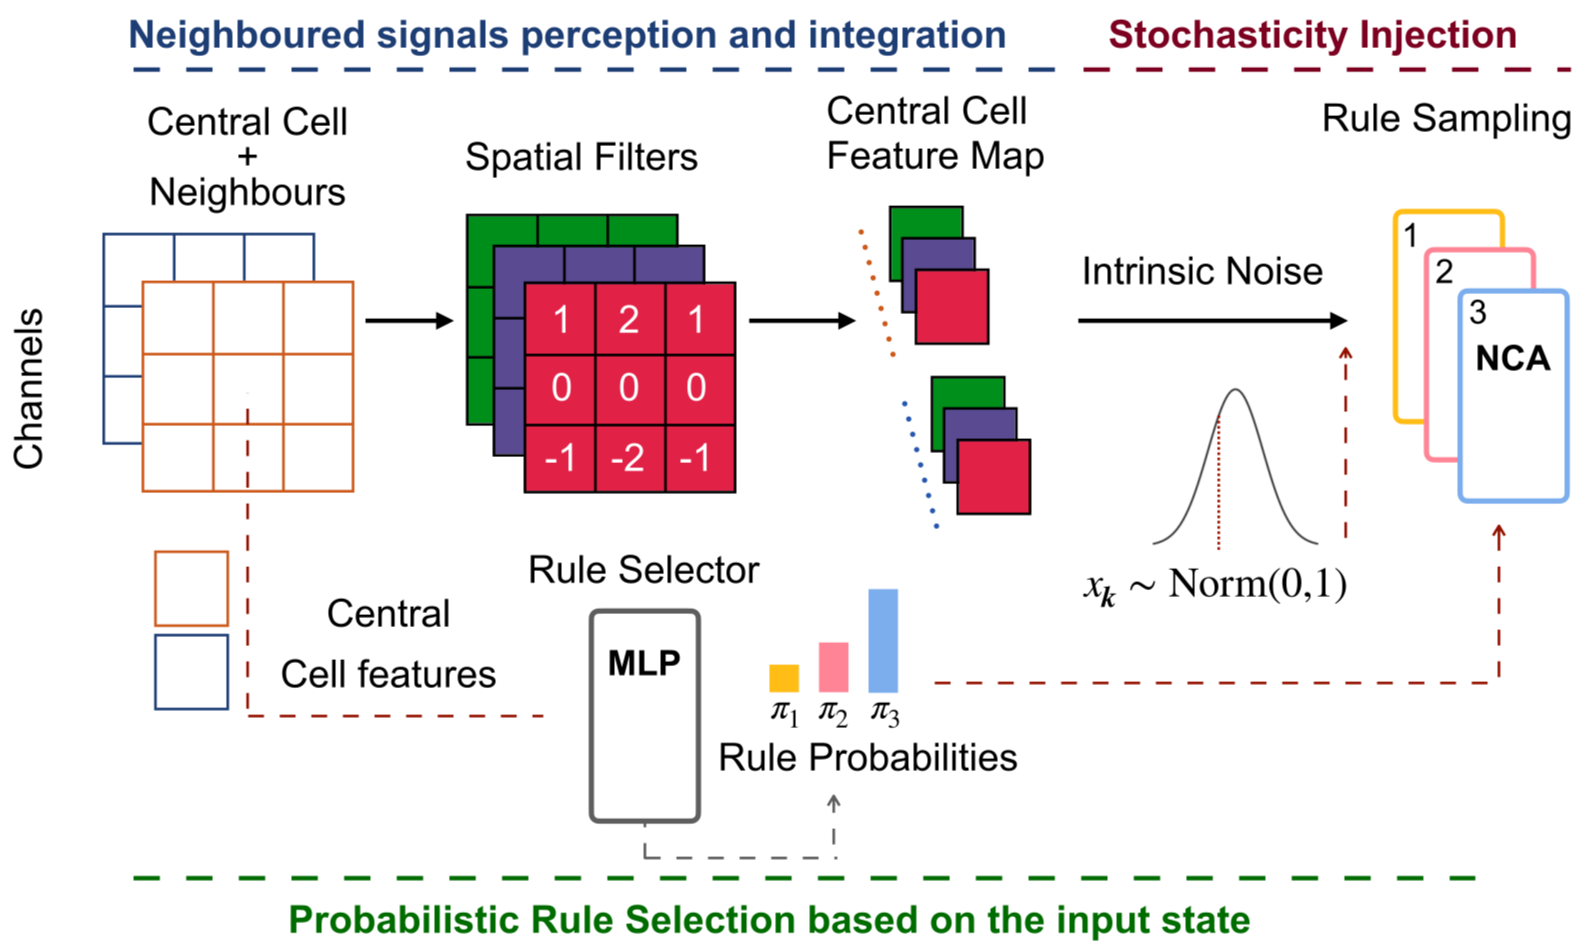
\includegraphics[width=0.76\textwidth]{figs/sota_mnca_schema}
  \caption{MNCA architecture. \textbf{Legend:} perception (central cell + neighbours) \(\rightarrow\) rule selector (MLP) \(\rightarrow\) rule probabilities; selected rule applied to perceived state; optional noise \(x_k\) for intrinsic-noise variant.}
  \label{fig:sota:mnca_schema}
\end{figure}

\subsection{Experimental evidence and interpretability}

The paper evaluates MNCA in three domains.
\begin{itemize}
  \item \textbf{Synthetic tissue growth and differentiation:} a stochastic simulator generates epithelial-like tissues with five cell types (stem, two intermediate, two differentiated) on a \(35\times 35\) grid from an initial cluster of stem cells. MNCA and MNCA with intrinsic noise are trained to reconstruct the state at each time step. They substantially outperform a deterministic NCA and a Gaussian NCA (GCA)~\cite{gnca_jeandelle2024} in terms of KL divergence of the cell-type distribution, Wasserstein distance on tissue size, and Wasserstein distance on border complexity, following recent practice in using Wasserstein-based metrics in machine learning~\cite{arjovsky2017wasserstein}. For example, the deterministic NCA reaches a KL divergence of about 2.06 while MNCA reaches about 0.02; the model with intrinsic noise further improves border fidelity \cite{mnca_milite2025}. Moreover, the learned rule assignments align with cell types: plotting the probability of each rule across the grid shows that roughly one rule is associated with each cell type (and one with empty space), with some rules shared (e.g.\ stem and one differentiated type), indicating that the model has discovered an interpretable partition of the state space.
  \item \textbf{Image morphogenesis:} the model is trained on emoji-like target images (as in Mordvintsev et al.) and then tested \emph{without} having seen perturbations during training. Under chunk removal, Gaussian noise addition, and sparse pixel removal, mixture-based NCAs recover the target image more reliably than the deterministic NCA; the error over recovery steps often peaks then decreases, suggesting that the target acts as an attractor. The GCA baseline does not show a clear advantage over the deterministic NCA in these experiments.
  \item \textbf{Unsupervised segmentation of microscopy images:} using high-content screening data (BBBC031v1), the authors initialise one seed per cell centroid and run the MNCA. The inferred rule assignments segment the tissue into regions that correlate with morphological and proteomic features (e.g.\ a provided ``cell shape parameter''), and constraining which rules are active at inference time can steer the population toward different phenotypes.
\end{itemize}
Together, these results support the claim that MNCA captures diverse local behaviours, improves robustness, and provides interpretable rule-based segmentation \cite{mnca_milite2025}.

\subsection{Motivations and advantages}

MNCA provides \emph{spatial heterogeneity}: different regions of the grid can specialise to different rules (e.g.\ by cell type or by position). It also provides \emph{temporal stochasticity} through both the random choice of rule and, in the noisy variant, the internal noise \(x_k\). This aligns with the view that biological cells exhibit context-dependent and inherently noisy behaviour. From a modelling perspective, the mixture can represent distinct behavioural programmes (proliferation, quiescence, differentiation) that are selected or mixed according to local state. From an interpretability perspective, the rule-assignment maps allow one to see how the model partitions the grid into functional regions and to relate those partitions to known biological or morphological structure. Finally, the explicit stochasticity and multiplicity of rules make MNCA a better fit for biological growth and self-organisation than a single deterministic NCA \cite{mnca_milite2025}. In this thesis we adopt MNCA as the base model and study how its behaviour changes when we vary the spatial neighbourhood size.

%-------------------------------------------------------------------
\section{Hierarchy in Self-Organising Systems and in NCA}
\label{sec:sota:hierarchy}
%-------------------------------------------------------------------

Biological systems are organised at multiple scales: cells form tissues, tissues form organs, and organs form organisms. Communication and control occur both within and across these scales. A single-scale NCA models dynamics at one level (e.g.\ cells on a grid) and does not explicitly represent higher-level structure (tissues, organs) or feedback from larger scales to smaller ones.

Hierarchical NCA (H-NCA) \cite{hnca_pande2023} addresses this by arranging several NCA modules in a hierarchy. Each cell of an NCA at a higher level is associated with a \emph{cluster} of cells of the NCA at the level below. The higher-level cell receives a summary of the state of its cluster (via a sensor) and can influence the lower-level NCA through signal channels (via an actuator). Training is phased: the lower-level NCA is trained toward its own goal; once it reaches a stable state, feedback is sent to the level above, which then modulates the lower level. This allows the system to exhibit multi-phase behaviour (e.g.\ growth then differentiation) and to model phenomena such as cell differentiation and metamorphosis, where the trigger for a new phase comes from within the system rather than from an external controller. The authors show that such hierarchical organisation can improve the capacity to evolve and maintain complex patterns and to coordinate behaviour across scales \cite{hnca_pande2023}. \Cref{fig:sota:hnca_arch} illustrates the H-NCA layout.

\begin{figure}[t]
  \centering
  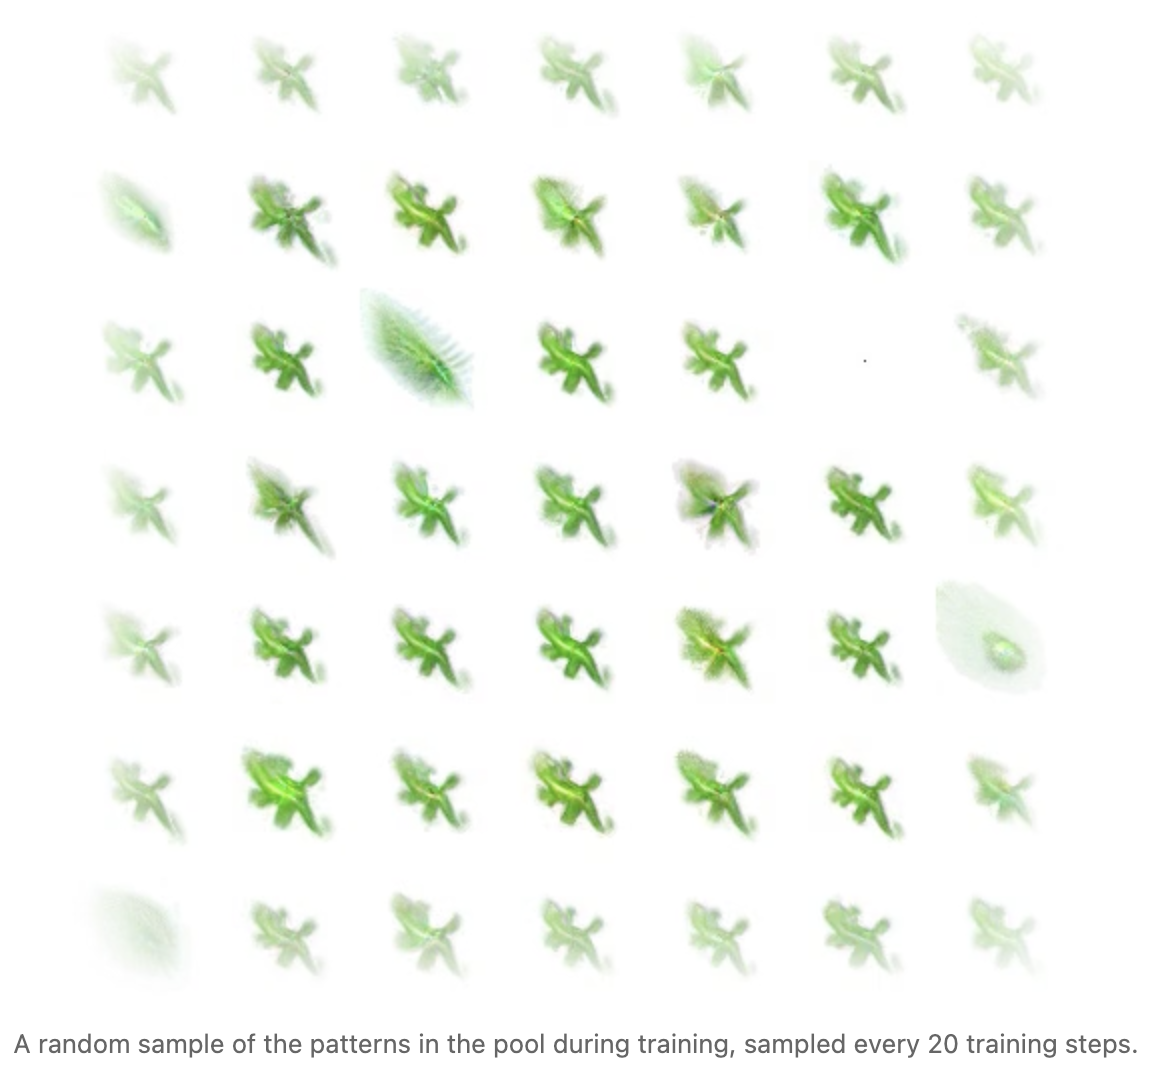
\includegraphics[width=0.72\textwidth]{figs/sota_hnca_architecture}
  \caption{H-NCA. \textbf{Legend:} parent NCA cells each control a cluster of child NCA cells; sensor (child\(\rightarrow\)parent) and actuator (parent\(\rightarrow\)child) mediate feedback. Adapted from Pande et al.~\cite{hnca_pande2023}.}
  \label{fig:sota:hnca_arch}
\end{figure}

Although hierarchical NCA is not directly used in the experiments of this thesis, it provides a broader perspective on the literature: the MNCA model adopted here operates at a single scale with multiple rules; future work could combine mixture-style stochasticity with hierarchical structure to capture both heterogeneity at one scale and coordination across scales.

%-------------------------------------------------------------------
%\section{Connections to Topological Deep Learning}
%\label{sec:sota:topological}
%-------------------------------------------------------------------

% (Discussion of topological deep learning moved to future work; see \cref{sec:conc:future}.)

%-------------------------------------------------------------------
\section{Synthesis and Positioning of This Thesis}
\label{sec:sota:synthesis}
%-------------------------------------------------------------------

In summary, the literature shows a clear progression. Classical cellular automata establish that local rules suffice for emergent global behaviour but leave the rule design to the modeller; inverse design remains difficult. Neural cellular automata address this by learning the rule from data while preserving locality and differentiability; the link between CA and convolutional networks was established by Gilpin \cite{ca_gilpin2019}, and learning from data for morphogenesis was demonstrated by Mordvintsev et al.\ \cite{nca_mordvintsev2020}. Growing NCA specialises the framework to growth from a seed and introduces training strategies (sample pool, damage) for persistence and regeneration. Standard NCA, however, remain deterministic and single-rule, which limits their ability to capture the variability and heterogeneity observed in real biological systems. Mixture NCA extend the framework by introducing multiple rules and stochastic selection, aligning the model with the stochastic, heterogeneous nature of real tissues; the work of Milite et al.\ provides a formalisation and empirical validation across tissue growth, image morphogenesis, and microscopy segmentation. Parallel developments include hierarchical NCA for multi-scale organisation; related ideas from topological deep learning for data on non-Euclidean or higher-order structures are discussed as a direction for future work in \cref{sec:conc:future}. Taken together, this body of work motivates the use of MNCA as the base model for the present thesis.

The contribution of this thesis sits squarely on the MNCA branch: the mixture formulation is taken as given, and the central question is whether enlarging the spatial neighbourhood improves performance in a tissue-growth setting. The hierarchy and the topological formulation of the domain are not modified; the focus is on the effect of the locality radius and on the interaction between neighbourhood size, curriculum design, and long-horizon stability. The following chapters describe the tools, the implementation, and the results of that investigation.

%-------------------------------------------------------------------
\chapter{Tools and Frameworks}
\label{c:tools}
%-------------------------------------------------------------------

\epigraph{\enquote{I believe that inside every tool is a hammer.}}{\emph{Adam Savage}}

This chapter describes the tools and frameworks used in the thesis.

%----------------------------------------------------------
\section{Software stack}
%----------------------------------------------------------

The experiments in this thesis are implemented in Python.
Most model components are implemented with \texttt{PyTorch}, while data manipulation and analysis use standard scientific libraries (e.g., \texttt{NumPy}, \texttt{pandas}, \texttt{matplotlib}).
Interactive exploration and plotting were done in an interactive environment, while long experiment runs were executed via reproducible command-line pipelines.

\paragraph{Reproducibility and artifacts.}
To make experiments easier to reproduce and inspect, the pipeline saves:
(i) trained model checkpoints (e.g., \texttt{.pt} files),
(ii) datasets as serialized arrays (for reproducibility),
(iii) per-configuration metrics as \texttt{.csv},
and (iv) plots and dashboards as static images or \texttt{.html} reports.

%----------------------------------------------------------
\section{Code organization}
%----------------------------------------------------------

The repository is organized around a few core components:

\begin{itemize}
\item \textbf{Models:} implementations of NCA and mixture-based extensions are in \texttt{mix\_NCA/}.
\item \textbf{Synthetic biological simulator:} a biologically-inspired toy simulator is used to generate supervised tissue-growth trajectories.
\item \textbf{Experiment pipeline:} automated training/evaluation sweeps with standardized outputs (checkpoints, metrics, plots).
\item \textbf{Analysis pipeline:} aggregation and visualization code that produces the final dashboards used in the thesis.
\end{itemize}

In particular, the neighborhood-size sweep discussed in \cref{c:implementation} uses a pre-generated dataset of simulated histories plus the metrics and checkpoints produced by the sweep runs.

%----------------------------------------------------------
\section{Compute and execution}
%----------------------------------------------------------

Training is GPU-friendly but not strictly required: the code can fall back to CPU execution.
Where available, the implementation supports selecting the best backend automatically (CUDA, Apple MPS, or CPU).
For longer training horizons (hundreds of rollout steps), computational cost is mainly dominated by repeated unrolls of the learned dynamics, so experiment design (dataset size, rollout horizon, and curriculum schedules) plays an important role in iteration speed.

%-------------------------------------------------------------------
\chapter{Implementation}
\label{c:implementation}
%-------------------------------------------------------------------

\epigraph{\enquote{Sometimes, the elegant implementation is just a function. Not a method. Not a class. Not a framework. Just a function.}}{\emph{John Carmack}}

This chapter shows the details of the implementation of the work.

%----------------------------------------------------------
\section{How experiments are structured}
%----------------------------------------------------------

The experimental work in this thesis is organized as a sequence of increasingly controlled studies.
The main research question is whether increasing the \emph{spatial neighborhood size} (\(NB\)) in Mixture Neural Cellular Automata improves long-horizon behavior in a tissue-growth setting.
In practice, the experiments are implemented as training/evaluation pipelines that can be repeated across multiple neighborhood sizes, while keeping all other hyperparameters fixed whenever possible.

At a high level, each experiment follows the same steps:
\begin{itemize}
\item generate or load a dataset of tissue-growth trajectories (``histories'');
\item train one or more NCA variants on short temporal windows extracted from these histories;
\item evaluate the trained models by running free rollouts (no teacher forcing) for different horizons;
\item compute quantitative metrics and inspect qualitative rollouts.
\end{itemize}

%----------------------------------------------------------
\section{Data generation and biological toy model}
%----------------------------------------------------------

Before training NCAs, we need supervised trajectories representing plausible tissue dynamics.
In this thesis, these trajectories are generated by a simple stochastic, biologically-inspired simulator and collected through a small data-generation pipeline.

\paragraph{State representation (cell types).}
Each simulation state is a 2D grid of discrete cell types.
In the ``complex'' configuration used for most experiments, the simulator includes a small differentiation hierarchy (e.g., \texttt{STEM}, \texttt{INTERMEDIATE}, and \texttt{DIFFERENTIATED} types), plus an \texttt{EMPTY} background.

\paragraph{Local update rules (biological intuition).}
At each simulation step, each occupied cell can:
(i) die, (ii) survive, or (iii) divide into a nearby empty site.
When a division happens, the newly created cell may \emph{differentiate} according to a probability table that depends on the parent cell type and (optionally) on neighbor context.
This yields trajectories that show growth, spatial organization, and gradual maturation into differentiated compartments.

\paragraph{Histories.}
For a single simulation we record the entire time series of grids \(x_0, x_1, \dots, x_T\).
We refer to this time series as a \emph{history}.
In the thesis we may visualize a history either as a sequence of snapshots (selected time points) or as a small montage, because it helps identify qualitative behaviors (stable growth, collapse, frozen patterns, etc.).

\paragraph{Dataset definition.}
Formally, the dataset is a collection of histories:
\[
\mathcal{D}=\{x^{(i)}_{0:T}\}_{i=1}^{N},
\]
where each \(x^{(i)}_t\) is a discrete 2D grid state at time \(t\).
In this work we use multiple datasets with different \(N\) and \(T\) depending on the experiment.

\paragraph{How a single history is generated (example).}
To generate one history, we start from an initial condition where a small cluster of stem-like cells is placed near the center of the grid (with small randomness), while all other sites are empty.
Then, for each time step, cells update locally:
each occupied site may die, survive, or divide into a nearby empty site; if a division occurs, the newly created cell may differentiate according to a type-dependent probability table that can also be influenced by the local neighborhood composition.

The goal is not to perfectly match biology, but to produce trajectories with growth and spatial organization that can serve as supervised targets for learning a local update rule.

\begin{figure}[t]
  \centering
  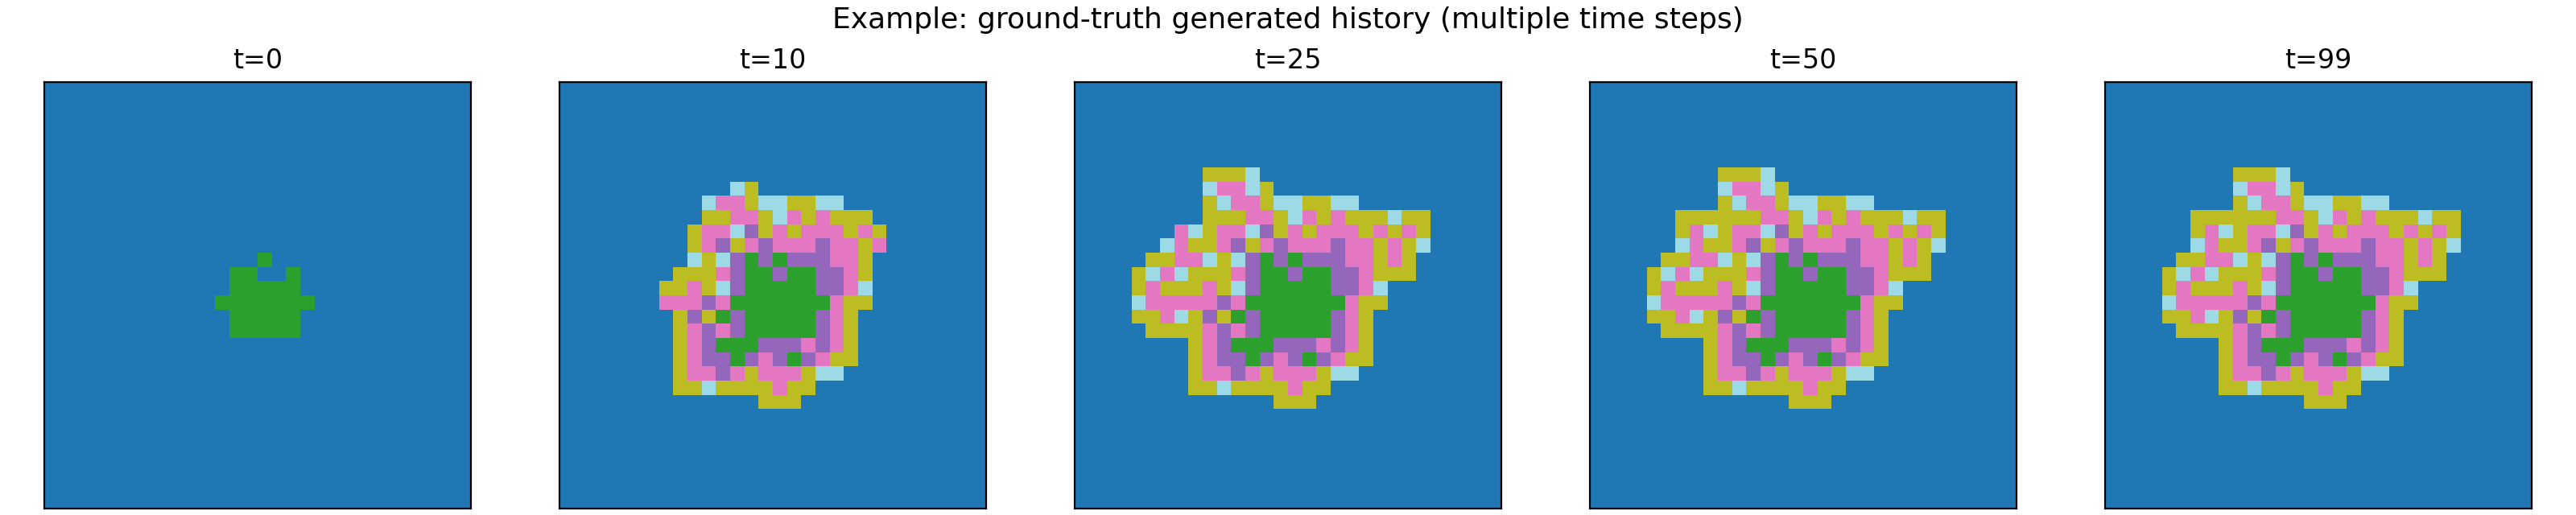
\includegraphics[width=\textwidth]{figs/tissue_examples/history_generation_example.png}
  \caption{Example of a generated history (ground truth) shown at multiple time steps. Each panel is a snapshot of the same simulation at a different time point.}
  \label{fig:impl:data:history_example}
\end{figure}

\paragraph{Datasets used in this thesis.}
Different experiments used different history datasets.
For instance, the final neighborhood sweep uses a dataset of 300 simulated trajectories with a horizon of 100 time steps (stored as a serialized array for reproducibility).

%----------------------------------------------------------
\section{Model training: from trajectories to learned update rules}
%----------------------------------------------------------

All NCA-style models in this thesis learn a \emph{local} update rule that is applied repeatedly over time.
Conceptually, a standard formulation is:
\begin{equation}
x_{t+1} = x_t + f_{\theta}\!\left(\mathcal{P}(x_t)\right),
\end{equation}
where \(x_t\) is the grid state at time \(t\), \(\mathcal{P}(\cdot)\) is a local perception operator (it extracts neighborhood information), and \(f_{\theta}\) is a neural network that predicts an update.
Mixture models extend this idea by having multiple candidate update rules and a learned mechanism to select (or mix) them over space and time \cite{mnca_milite2025}.

In training, the models are usually optimized on short temporal windows extracted from longer histories (teacher-forced supervision), while evaluation is performed as free-running rollouts.
This gap is important when we compare neighborhood sizes, because a low short-horizon loss does not automatically imply stable long-horizon behavior.

\paragraph{Example of generation by the learned model (multi-step rollout).}
After training, we can use a model to generate a trajectory by starting from an initial grid \(x_0\) and iterating the learned update rule for multiple steps, producing \(\hat{x}_1, \hat{x}_2, \dots, \hat{x}_T\).
Figure~\ref{fig:impl:model:rollout_example} shows an example rollout over multiple steps (same initial condition as \cref{fig:impl:data:history_example}), illustrating what it means for the model to ``free-run''.

\begin{figure}[t]
  \centering
  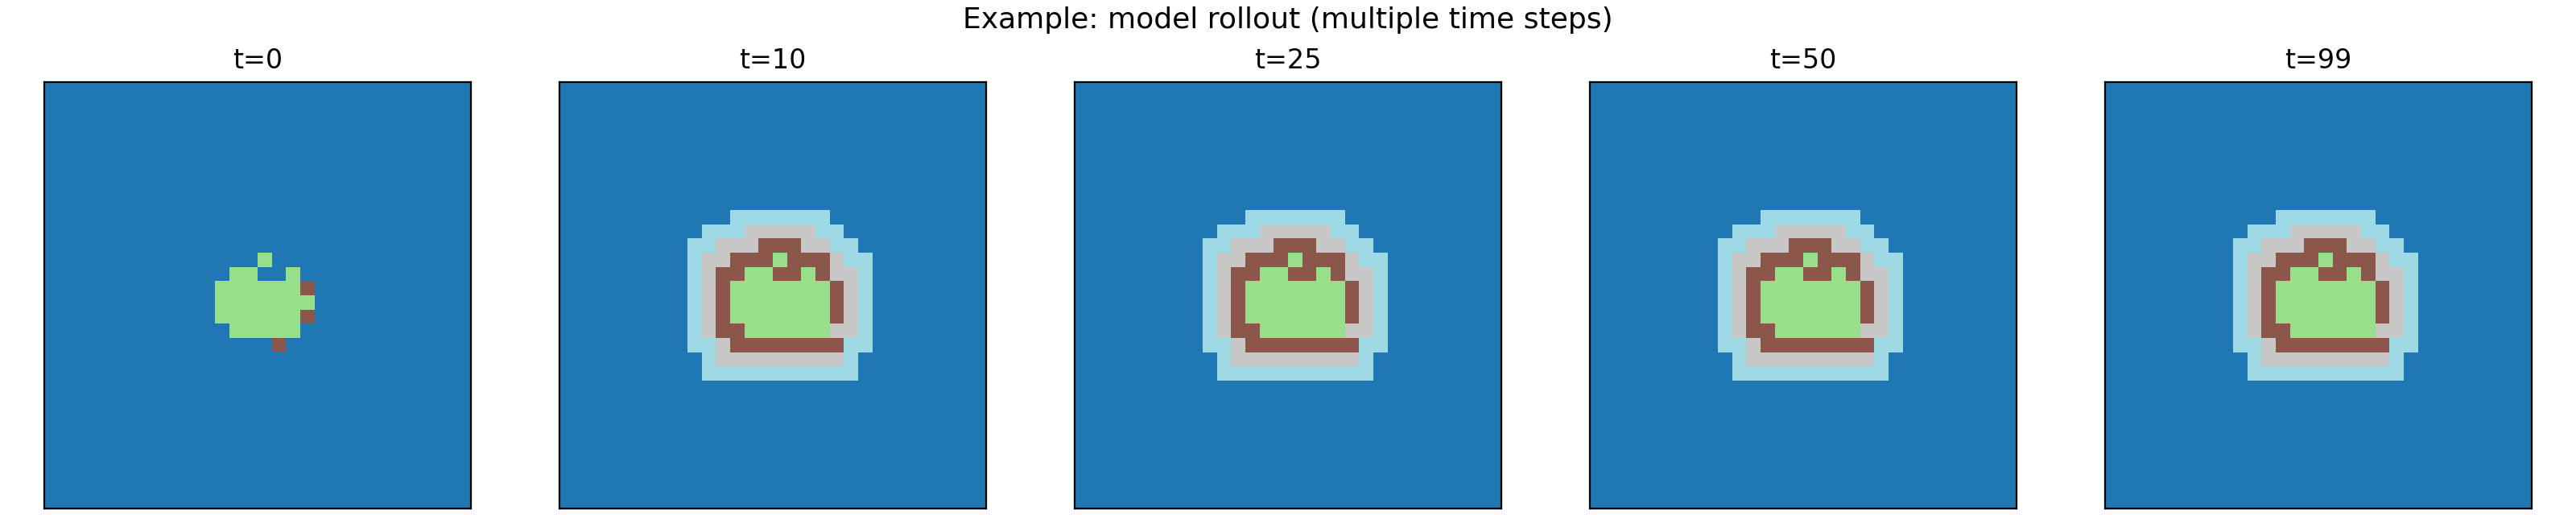
\includegraphics[width=\textwidth]{figs/tissue_examples/model_rollout_example.png}
  \caption{Example of a model-generated rollout over multiple steps, starting from the same initial condition used for the ground-truth history. This visualization helps qualitatively assess whether the learned dynamics remain stable when the model is run freely.}
  \label{fig:impl:model:rollout_example}
\end{figure}

\begin{figure}[t]
  \centering
  \begin{minipage}[t]{0.49\textwidth}
    \centering
    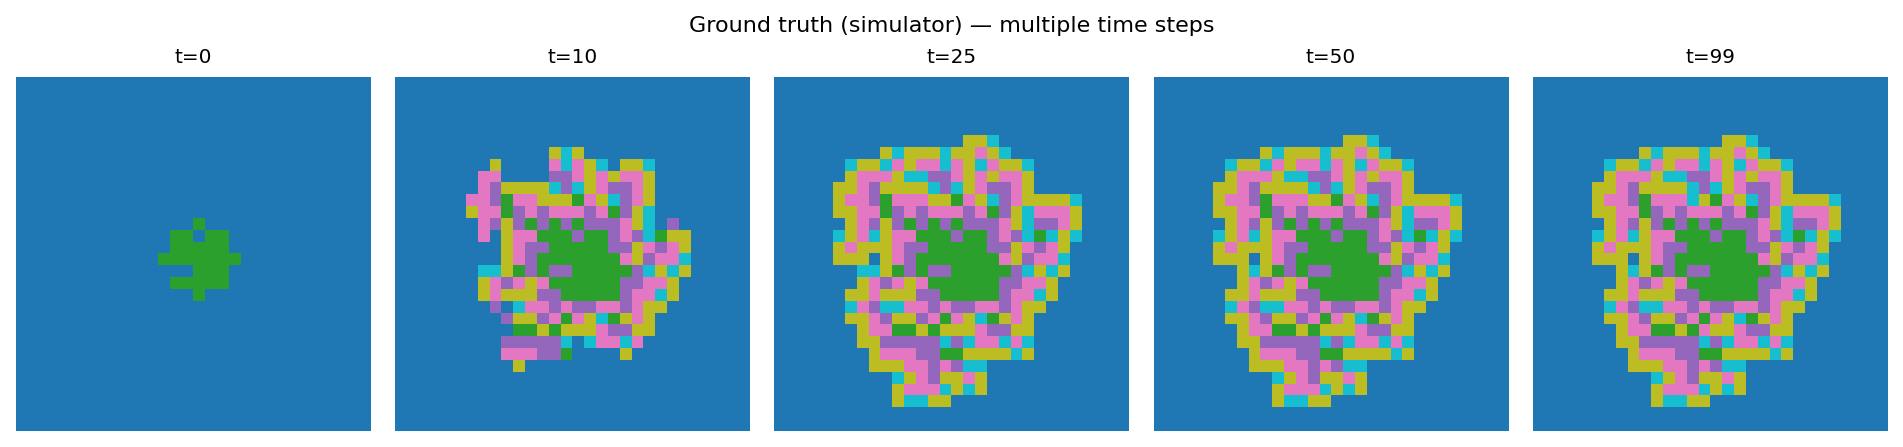
\includegraphics[width=\textwidth]{../presentation/assets/same_init/sample_149/ground_truth.png}
    
    {\small \textbf{Ground truth (simulator)}}
  \end{minipage}\hfill
  \begin{minipage}[t]{0.49\textwidth}
    \centering
    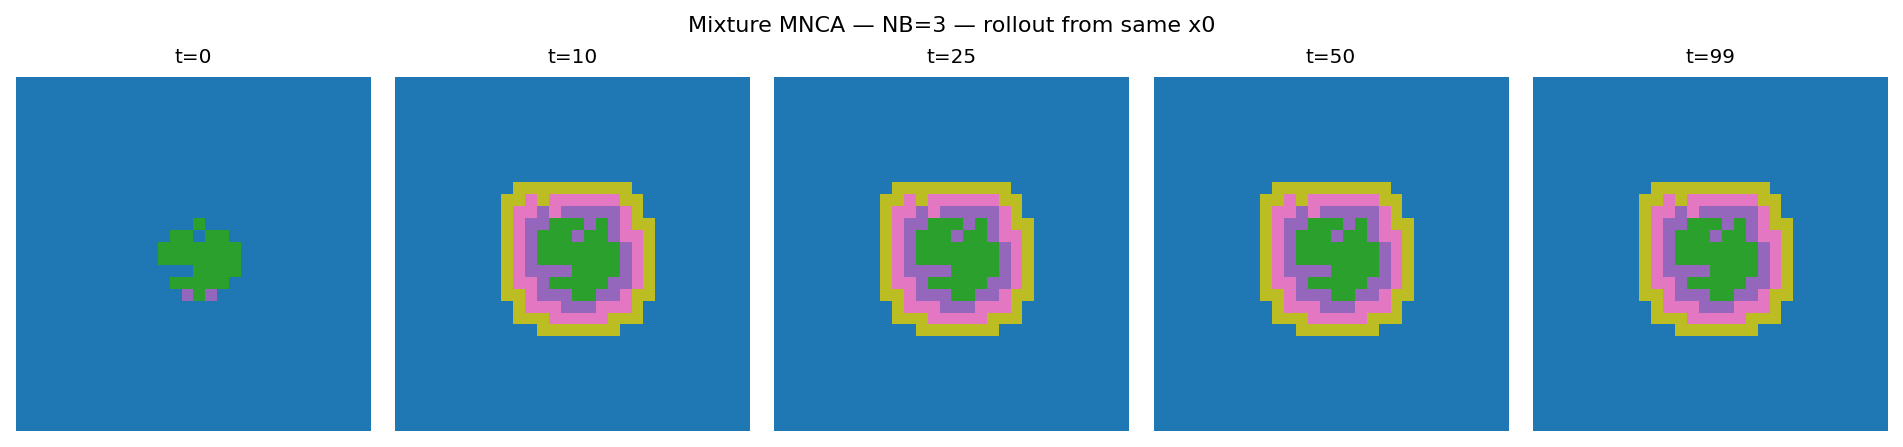
\includegraphics[width=\textwidth]{../presentation/assets/same_init/sample_149/mixture_nb_3.png}
    
    {\small \textbf{Model rollout (Mixture MNCA, NB=3)}}
  \end{minipage}
  \caption{Qualitative comparison on the same initial condition (sample 149): ground truth simulator history vs model-generated rollout. Both start from the exact same $t=0$ state.}
  \label{fig:impl:gt_vs_model_side_by_side}
\end{figure}

%----------------------------------------------------------
\section{Reference experimental setting from the original MNCA paper}
%----------------------------------------------------------

The starting point for our experiments is the training protocol used in the reference MNCA paper \cite{mnca_milite2025}.
In its ``paper-like'' regime, training uses a relatively small dataset and a short temporal horizon, with a long optimization schedule.
We replicate this setting as closely as possible and then change only the neighborhood size \(NB\), to isolate its effect.

%----------------------------------------------------------
\section{Experiment: does it make sense to extend the neighborhood?}
%----------------------------------------------------------

Our first experiment had a simple goal: understand whether extending the spatial neighborhood in MNCA is a meaningful direction.
We initially followed the paper-like regime, and then progressively changed the data and training schedule to strengthen supervision and make long-horizon training feasible.
Overall, the experiment was carried out in three steps (three configurations).

\subsection{Summary of steps 1 and 2}

We started from the training setup used in the reference paper: a relatively small dataset (\textbf{200 simulated trajectories}) with a short temporal horizon (\textbf{35 time steps}) trained for \textbf{800 epochs}.
Our first goal was not to change the learning procedure itself, but to isolate the effect of the \emph{spatial neighborhood size} (NB) by repeating the same training protocol across multiple neighborhoods.
In principle, increasing NB should allow the update rule to condition on a broader spatial context, which could improve regeneration and pattern stability.

In practice, this ``paper-like'' regime did not produce a clean answer to the neighborhood question.
Across several NB values, the qualitative rollouts remained inconsistent and the quantitative differences were small, making it hard to tell whether (i) NB genuinely had little impact, or (ii) the training signal was simply too weak/noisy in this low-data, short-horizon setting.
At that point, we were not confident that a negative result would be meaningful.

Following this, we attempted to strengthen the supervision by increasing both dataset size and sequence length, moving to \textbf{1000 trajectories of 500 time steps} each.
The motivation was twofold: (1) more trajectories reduce variance and improve coverage of initial conditions, and (2) longer sequences better represent the long-horizon behavior we ultimately care about when judging whether a model ``regenerates'' rather than just matching short-term transitions.
However, training directly on long sequences at this scale was computationally heavy and slowed iteration substantially.

To make long-horizon training feasible, we introduced \textbf{curriculum learning}, training on progressively longer temporal windows (e.g., a first phase with a \textbf{35-step} window, then \textbf{100-step}, and finally \textbf{500-step}, with fewer epochs and smaller learning rates in later phases).
The intended effect of the curriculum was to let the models first learn stable short-term local dynamics and then refine them under longer-horizon constraints without paying the full cost of long unrolls from the beginning.

Despite the curriculum, the resulting rollouts were often poor (the tissue failed to regenerate convincingly), which again prevented a meaningful comparison across neighborhood sizes.
At this stage we revisited the experimental pipeline and concluded that the main problem was not simply ``insufficient compute'', but \textbf{confounding factors that made the neighborhood sweep hard to interpret when the models were already failing}.
In particular, when training is dominated by short teacher-forced transitions while evaluation is performed as free-running rollouts, low training loss does not necessarily translate into good long-horizon behavior.
In addition, mixture models can behave very differently depending on whether rule selection is evaluated with soft (differentiable) assignments or hard sampling; if this is not kept consistent, the observed differences can be dominated by sampling behavior rather than by NB.

\subsection{Step 3: controlled neighborhood sweep (final configuration)}

For these reasons, we temporarily stepped back from the long-horizon curriculum experiment and adopted a more controlled ablation aimed specifically at answering the neighborhood-size question.
We fixed the ``extra'' degrees of freedom that can dominate dynamics (most importantly, keeping the rule-selection temperature effectively constant during the sweep and using a consistent sampling mode at evaluation), and we generated an intermediate dataset that is large enough for stability while still tractable (\textbf{300 trajectories, 100 time steps}).

We then evaluated each trained model at multiple rollout horizons (e.g., \textbf{25, 50, 100 steps}) rather than relying on a single horizon.
This produces a clearer picture: even if different NB values look similar at very short horizons, improvements from larger neighborhoods are expected to show up as slower degradation and better stability as the rollout length increases.

In summary, curriculum learning was introduced as a pragmatic response to the computational cost of training on \textbf{1000$\times$500} simulations.
We then reverted to a simpler setting not because the curriculum is ``wrong'', but because we first needed an interpretable experimental protocol where the neighborhood-size effect is not masked by optimization and sampling confounds.
Once a robust NB trend is established under controlled conditions, curriculum learning can be reintroduced as a second-stage validation on selected neighborhoods to confirm that the effect persists in the full long-horizon regime.

\paragraph{Where the results are reported.}
Since this configuration is part of the experimental \emph{pipeline design} (and it directly motivates our final protocol), we report its detailed results in this Implementation chapter.
The \cref{c:results} chapter instead focuses on the overall thesis conclusions.

\paragraph{High-level outcome (brief).}
Under this controlled protocol, the neighborhood-size effect becomes observable.
In our sweep over \(NB \in \{1,\dots,7\}\), \(NB=1\) is consistently inadequate, while moving to \(NB\ge2\) yields a clear improvement.
Beyond this first jump, improvements are not strictly monotonic: different neighborhood sizes trade off distributional agreement and spatial fidelity, and differences become more evident as the rollout horizon increases (e.g., 25 vs 100 steps).

%----------------------------------------------------------
\subsubsection{Step 3 results: evaluation protocol and key trends}
\label{sec:impl:step3:results}
%----------------------------------------------------------

We evaluate models trained with neighborhood sizes \(NB \in \{1,\dots,7\}\) using both \emph{distributional} and \emph{spatial} metrics computed on the final state of each generated simulation.
The reference dataset consists of 300 ground-truth histories with a horizon of 100 steps (stored as a serialized array for reproducibility).
For each neighborhood size, models are evaluated at multiple generation horizons (Step Length \(=25,50,100\)).
For each configuration we report aggregated performance (mean and variability across repeated evaluations) and we additionally inspect \emph{per-simulation} distributions to assess robustness and failure modes (heavy tails and outliers).

Figure~\ref{fig:impl:step3:dashboard} summarizes the overall trends across neighborhood sizes for the key metrics.
The main qualitative pattern is consistent across metrics: \(NB=1\) is systematically inadequate, while moving to \(NB\ge2\) yields a sharp performance improvement.
Beyond this first jump, increasing \(NB\) produces a non-monotonic trade-off between matching global distributions (e.g., KL divergence) and matching spatial structure (e.g., tumor size and border properties).

\begin{figure}[t]
  \centering
  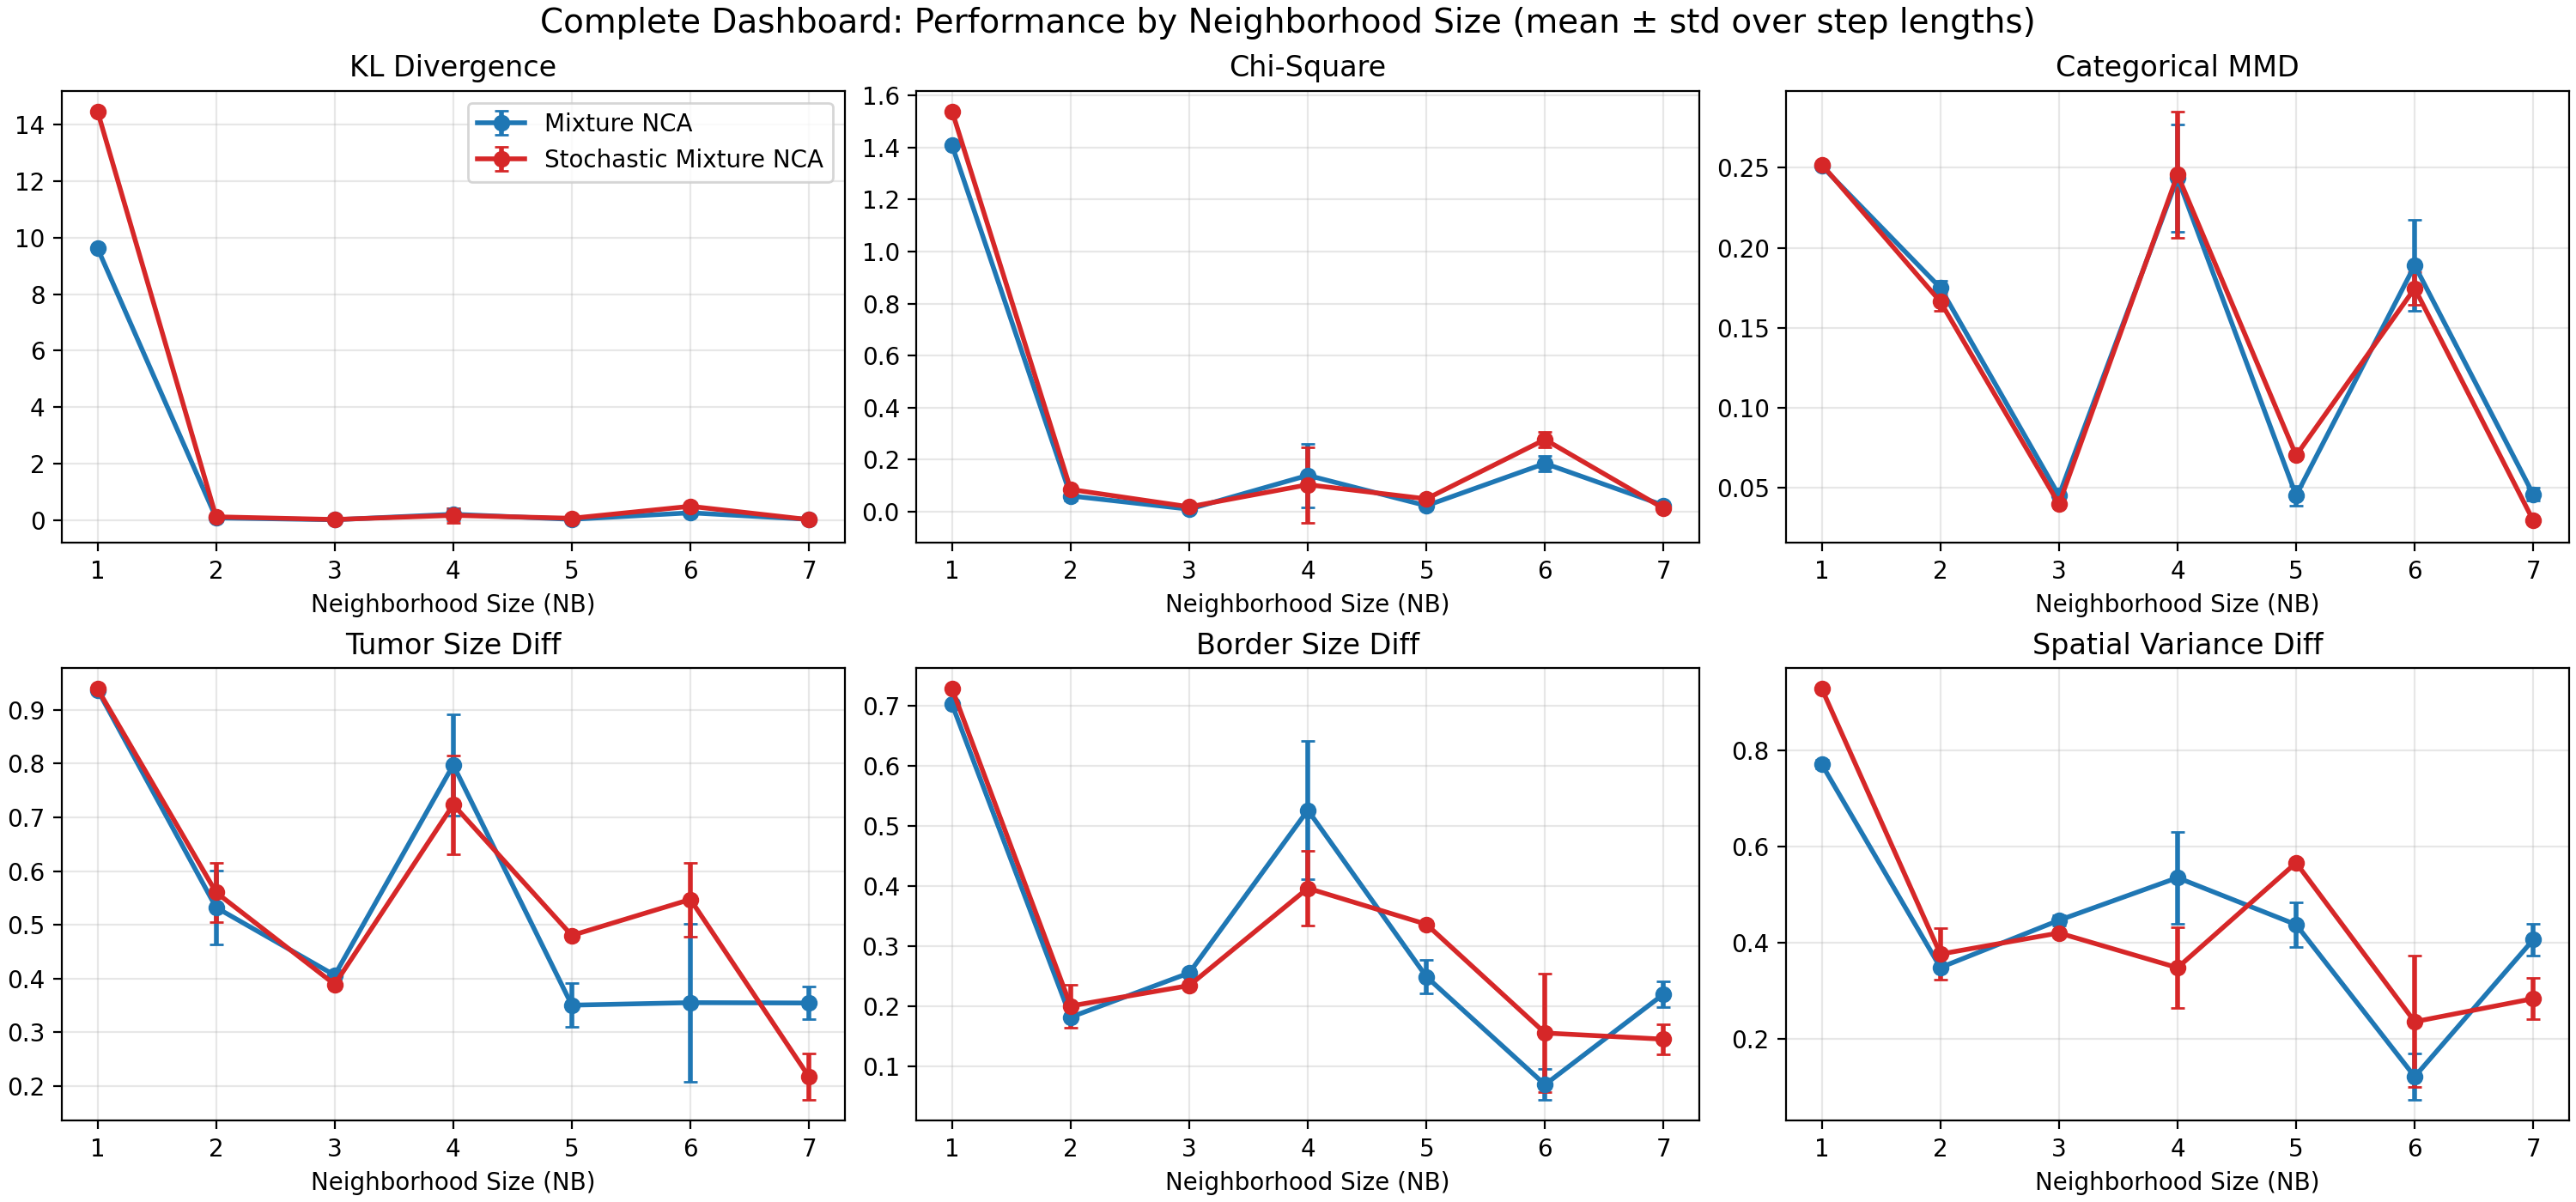
\includegraphics[width=\textwidth]{figs/neighborhood_analysis/nb_sweep_300x100/metrics_dashboard_full.png}
  \caption{Step 3: complete dashboard for the neighborhood sweep. We report mean and variability (standard deviation computed over the available step-length conditions) for the six metrics used in the analysis: KL divergence, Chi-square, categorical MMD, tumor size difference, border size difference, and spatial variance difference.}
  \label{fig:impl:step3:dashboard}
\end{figure}

%----------------------------------------------------------
\subsubsection{Distributional agreement and per-simulation variability}
\label{sec:impl:step3:kl}
%----------------------------------------------------------

KL divergence captures how well the global composition of cell types in the generated final state matches the empirical distribution from the dataset.
Across all step lengths, \(NB=1\) yields very large KL values, indicating a strong mismatch in global composition.
For \(NB\ge2\), both models reach low KL on average, but the best neighborhood can depend on the evaluation horizon and on whether rule selection is deterministic or stochastic.

To interpret robustness, we inspect \emph{per-simulation} distributions of the metrics using violin plots.
Compared to mean-only summaries, violins reveal heavy tails and outliers: these correspond to runs that converge to qualitatively wrong outcomes (failure modes), even when the median performance is competitive.

\begin{figure}[t]
  \centering
  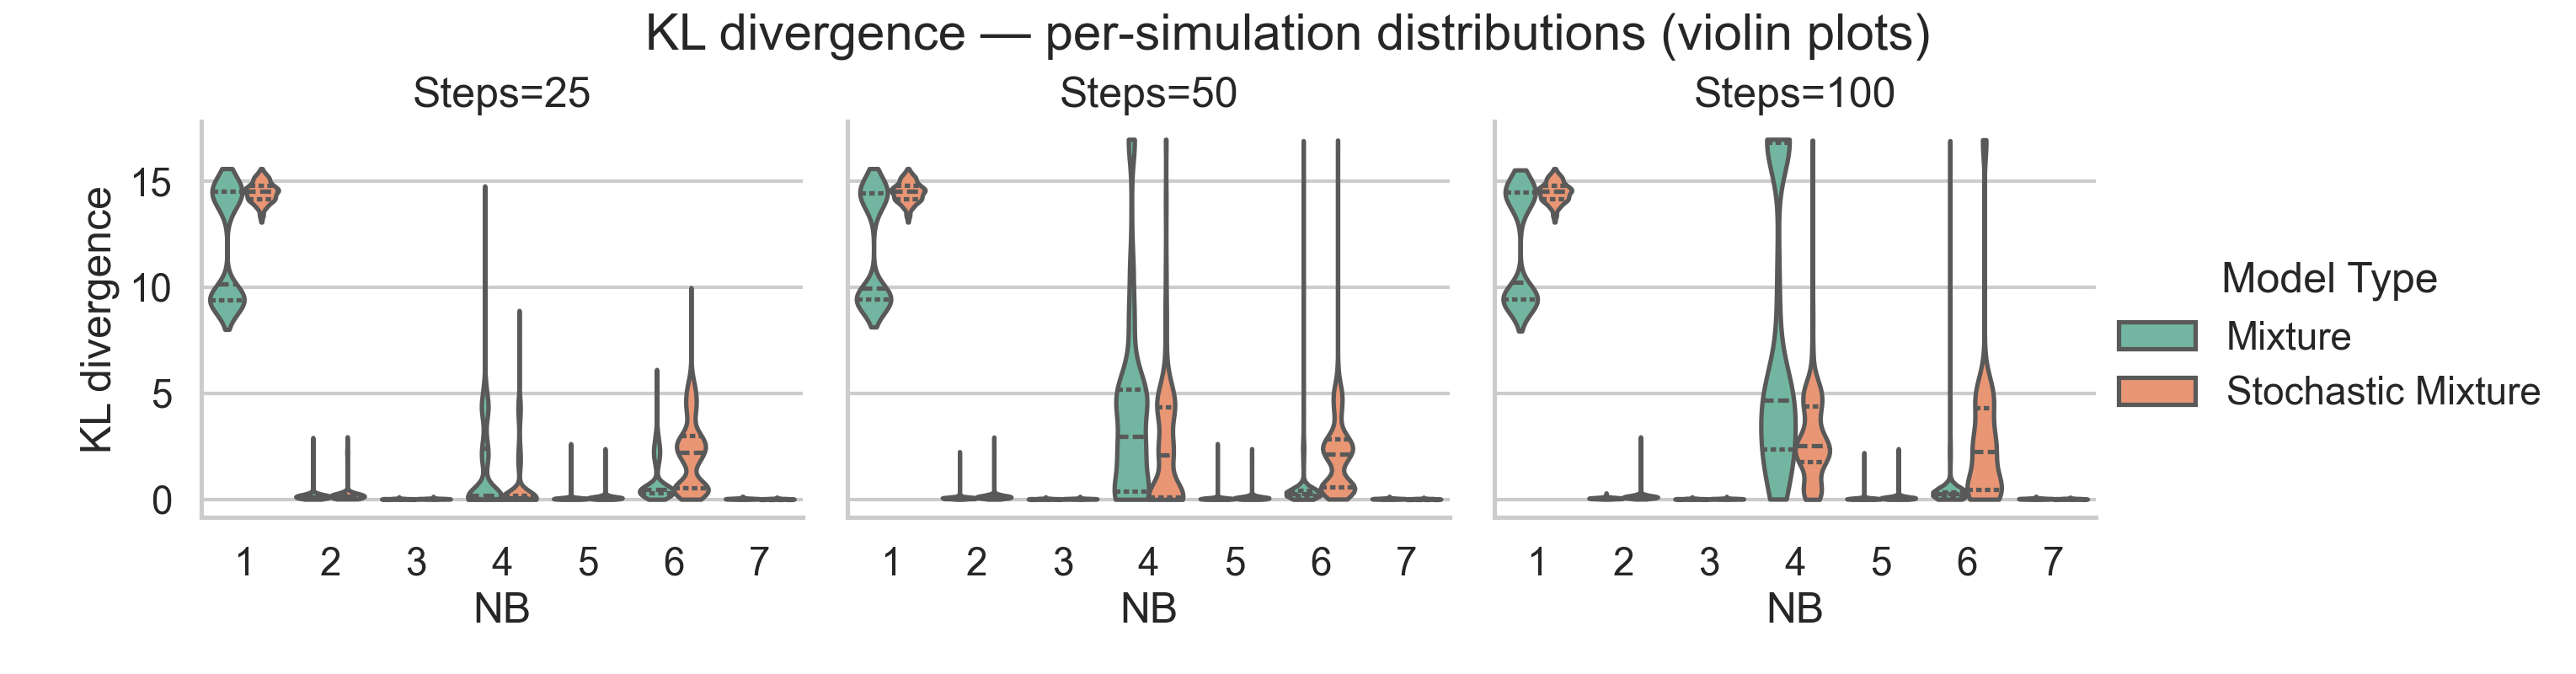
\includegraphics[width=\textwidth]{figs/neighborhood_analysis/nb_sweep_300x100/violin_KL_Divergence.png}
  \caption{Step 3: per-simulation violin plots for KL divergence (lower is better), faceted by step length. Violin width reflects density, and inner quartiles highlight robust central behavior; long upper tails indicate rare but severe failures that become more likely for specific neighborhood sizes and time horizons.}
  \label{fig:impl:step3:violin:kl}
\end{figure}

\begin{figure}[t]
  \centering
  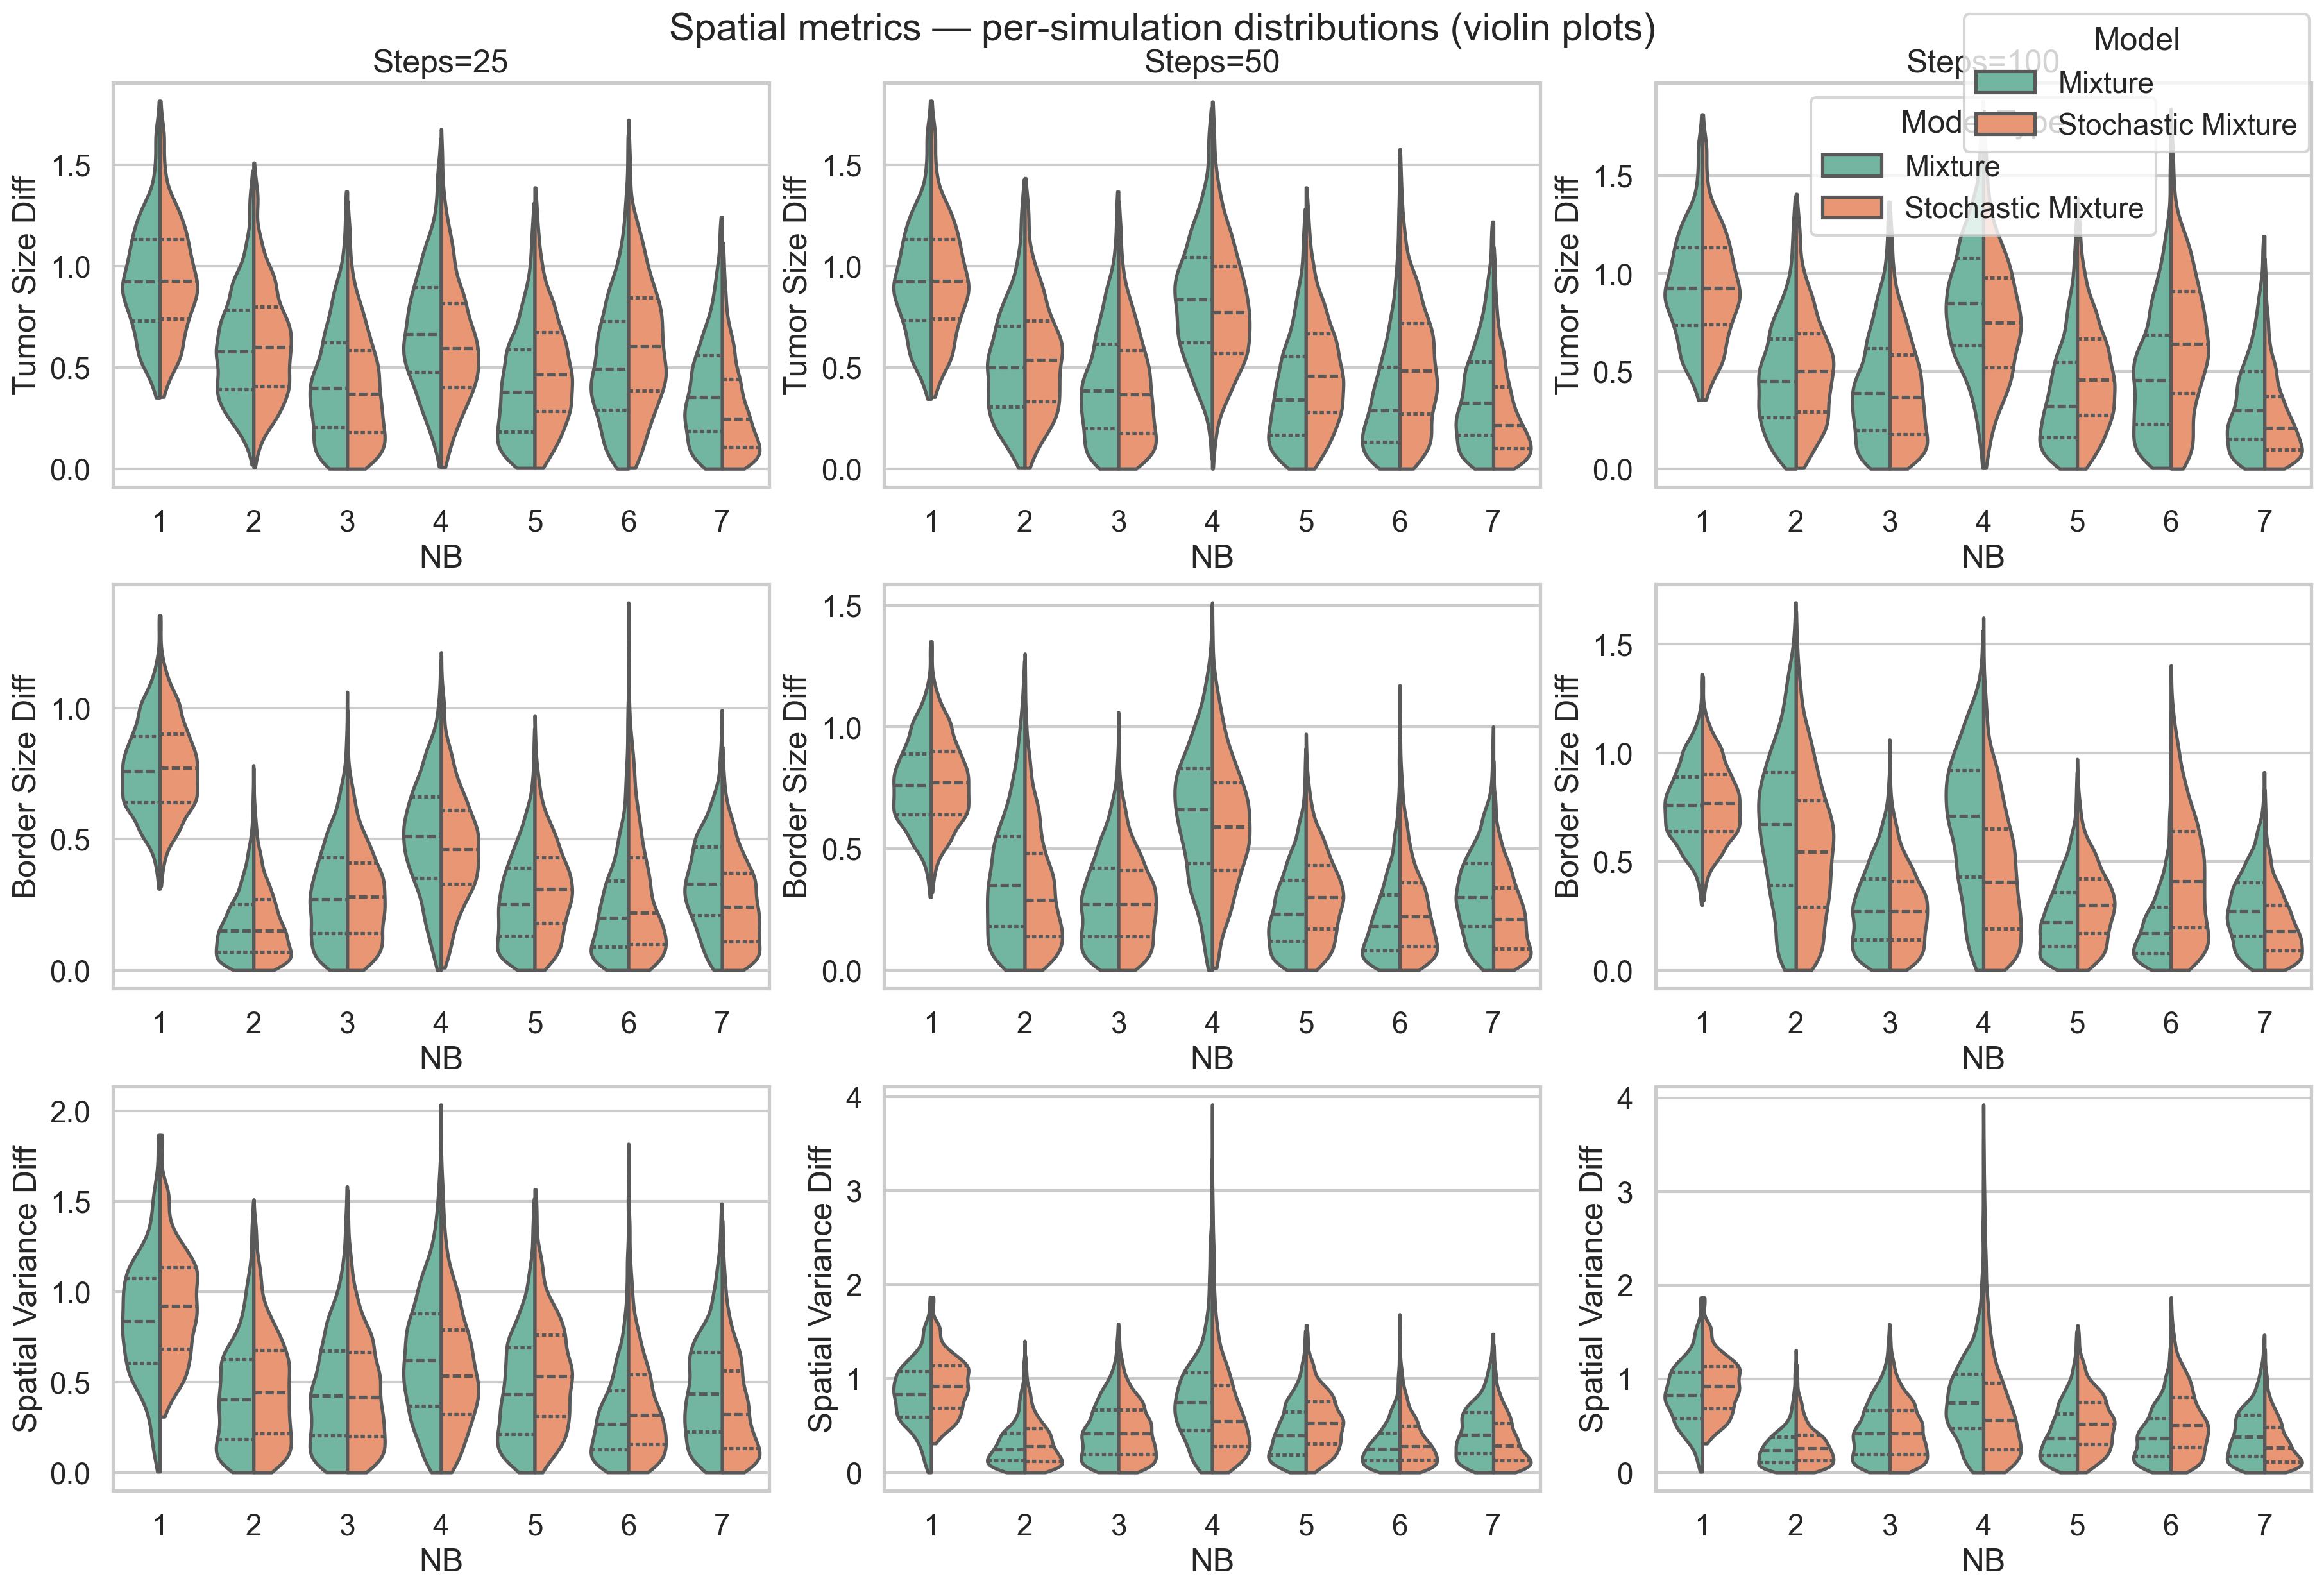
\includegraphics[width=\textwidth]{figs/neighborhood_analysis/nb_sweep_300x100/violin_spatial_metrics.png}
  \caption{Step 3: per-simulation violin plots for spatial metrics (tumor size, border size, spatial variance; lower is better), with one column per step length. This view complements mean trends by explicitly showing variability and tail risk as a function of neighborhood size.}
  \label{fig:impl:step3:violin:spatial}
\end{figure}

%----------------------------------------------------------
\subsubsection{Trend analysis and fold change}
\label{sec:impl:step3:trend}
%----------------------------------------------------------

To summarize how performance changes with neighborhood size in a compact way, we also compute a simple trend analysis over \(NB\).
In particular, we report fold change between a reference neighborhood (here \(NB=3\), used as a normalization point in the sweep) and a larger neighborhood (here \(NB=7\)).
This is useful because in several metrics the main effect is the jump from \(NB=1\) to \(NB\ge2\), while differences among \(NB\ge2\) are smaller and may depend on the metric.

\begin{figure}[t]
  \centering
  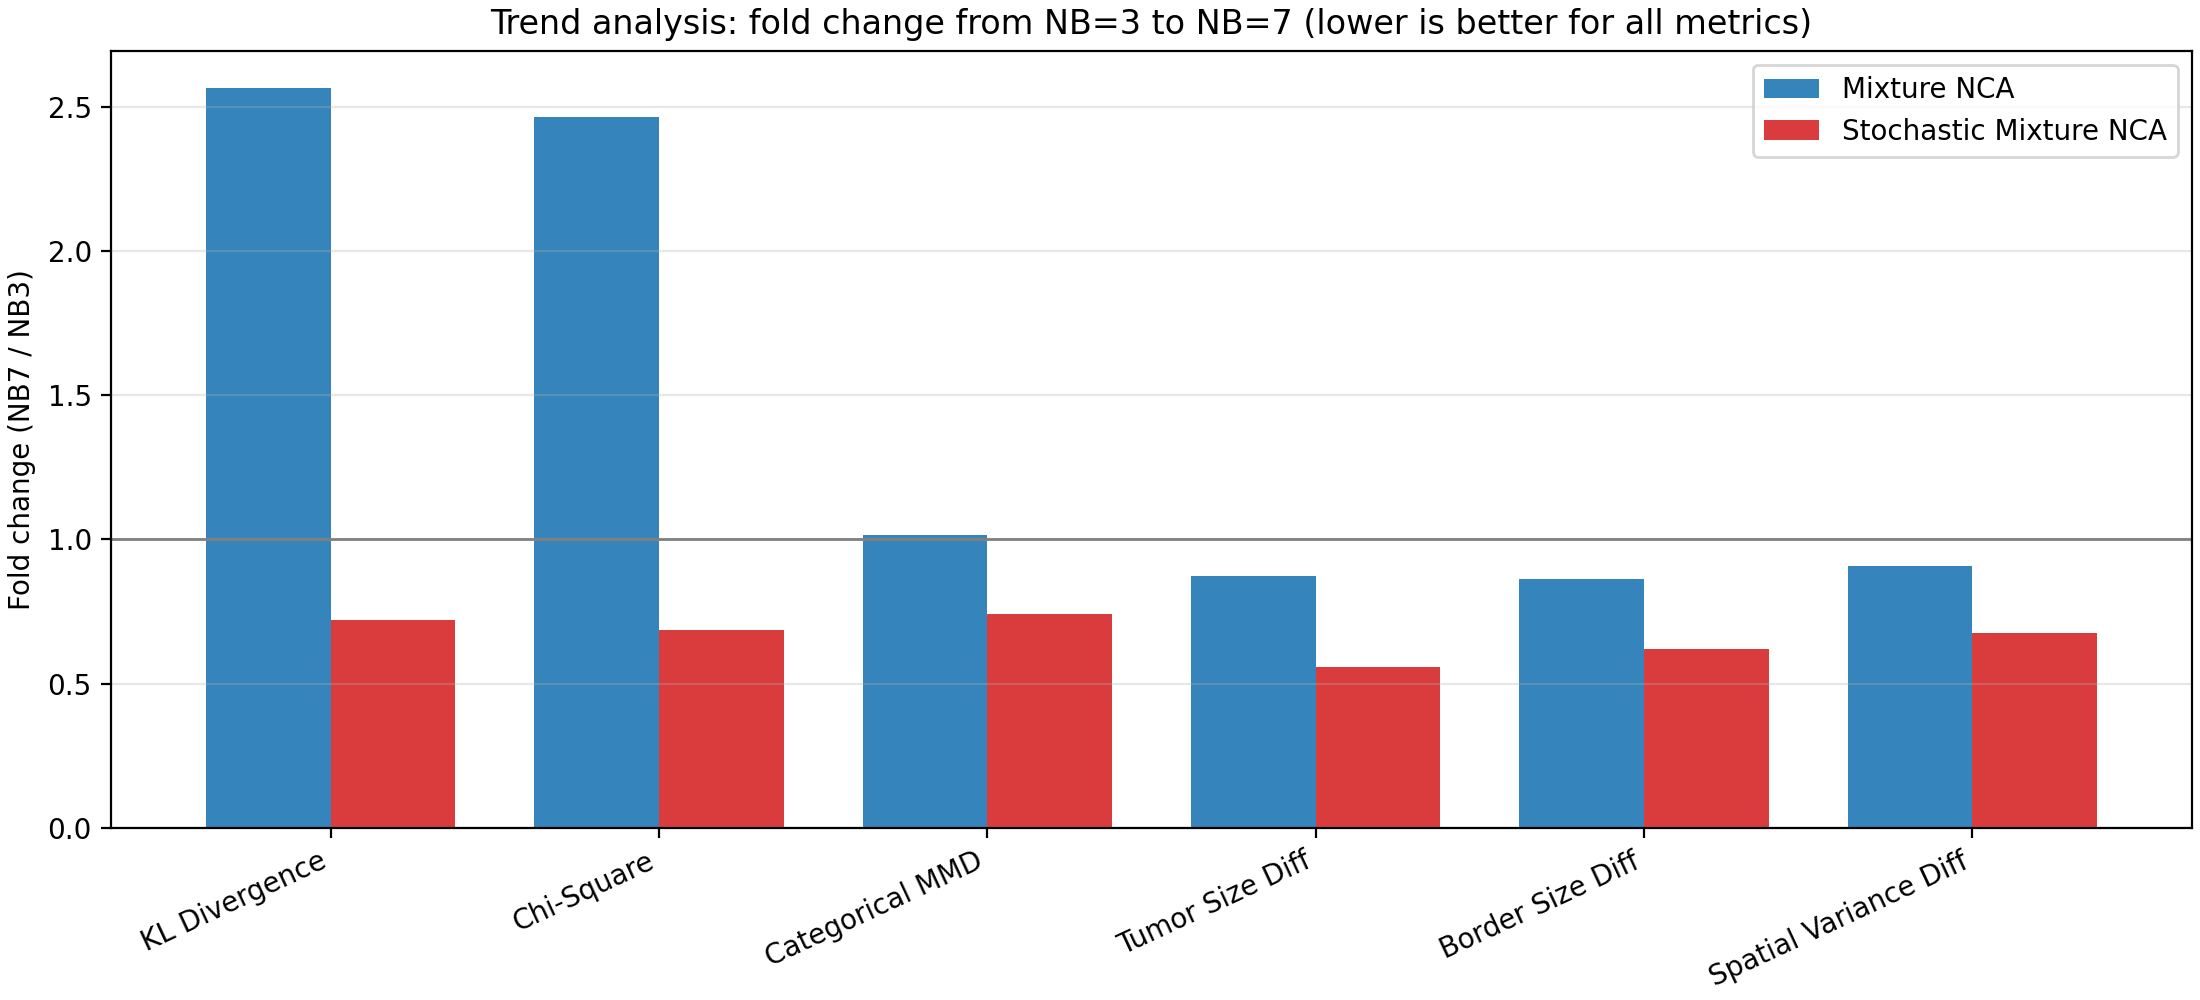
\includegraphics[width=\textwidth]{figs/neighborhood_analysis/nb_sweep_300x100/trend_foldchange_nb7_over_nb3.png}
  \caption{Step 3: trend analysis via fold change from \(NB=3\) to \(NB=7\) (ratio \(\\text{metric}(NB=7)/\\text{metric}(NB=3)\)). Values below 1 indicate improvement when increasing neighborhood size from 3 to 7, while values above 1 indicate degradation.}
  \label{fig:impl:step3:trend:foldchange}
\end{figure}

%----------------------------------------------------------
\subsubsection{Robustness via bad-rate}
\label{sec:impl:step3:badrate}
%----------------------------------------------------------

Mean values alone can hide important instability: per-simulation distributions often show heavy tails where a non-trivial fraction of runs ends in poor outcomes (``failure modes'').
To quantify this, we define a \emph{bad-rate} as follows: for each metric and each (model, step length), we select the neighborhood size with the best median performance, take the 95th percentile of that best distribution as a threshold, and compute for each \(NB\) the probability that a run exceeds this threshold.

\begin{figure}[t]
  \centering
  
\includegraphics[width=\textwidth]{figs/neighborhood_analysis/nb_sweep_300x100/badrate_bars_KL_Divergence.png}
  \caption{Step 3: bad-rate for KL divergence across neighborhood sizes (lower is better). Each bar reports the fraction of per-simulation runs whose KL exceeds the 95th percentile of the best-performing neighborhood for that (model, step length), highlighting robustness differences not visible in means alone.}
  \label{fig:impl:step3:badrate:kl}
\end{figure}

\begin{figure}[t]
  \centering
  
\includegraphics[width=\textwidth]{figs/neighborhood_analysis/nb_sweep_300x100/badrate_bars_Tumor_Size_Diff.png}
  \caption{Step 3: bad-rate for tumor size error (lower is better). Larger neighborhoods generally reduce the probability of severe failures for coarse morphology, especially for the stochastic variant.}
  \label{fig:impl:step3:badrate:tumor}
\end{figure}

\begin{figure}[t]
  \centering
  
\includegraphics[width=\textwidth]{figs/neighborhood_analysis/nb_sweep_300x100/badrate_bars_Border_Size_Diff.png}
  \caption{Step 3: bad-rate for border size error (lower is better). Border-related fidelity exhibits a trade-off: some intermediate neighborhood sizes may show heavier tails, indicating a higher chance of producing unrealistic borders even if the median performance is competitive.}
  \label{fig:impl:step3:badrate:border}
\end{figure}

\begin{figure}[t]
  \centering
  
\includegraphics[width=\textwidth]{figs/neighborhood_analysis/nb_sweep_300x100/badrate_bars_Spatial_Variance_Diff.png}
  \caption{Step 3: bad-rate for spatial variance error (lower is better). Spatial variance is particularly sensitive to step length and neighborhood size, showing that increasing \(NB\) can change both typical behavior and stability of the dynamics.}
  \label{fig:impl:step3:badrate:spvar}
\end{figure}

%----------------------------------------------------------
\subsubsection{Computational complexity and rule specialization}
\label{sec:impl:step3:complexity_rules}
%----------------------------------------------------------

Figure~\ref{fig:impl:step3:complexity} reports the empirical runtime as a function of neighborhood size.
In the explored range \(NB\in[1,7]\), the measured runtime remains approximately flat.
Empirically, Mixture NCA runs at about \(\sim 1.5\) ms/step on average, while the Stochastic Mixture variant is about \(\sim 3.2\) ms/step, with limited variation across neighborhood size.
This suggests that in this implementation range the practical cost is dominated by constants and vectorization effects rather than by the naive theoretical \(O(NB^2)\) scaling.

\begin{figure}[t]
  \centering
  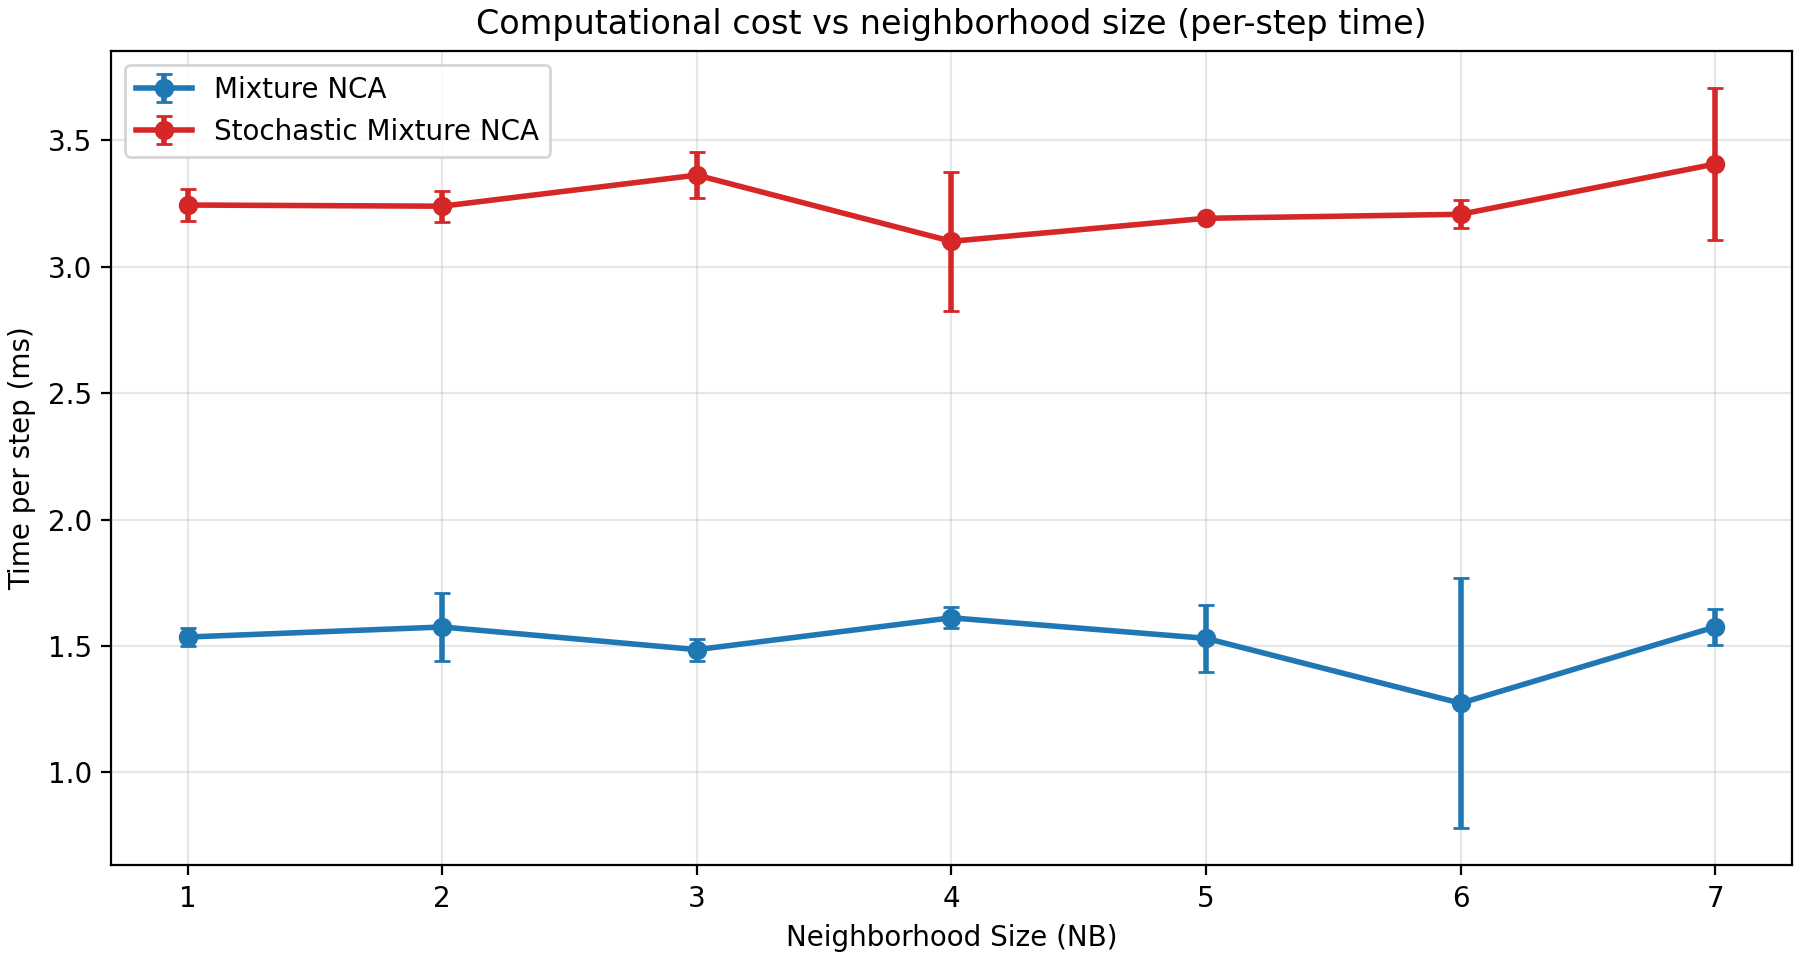
\includegraphics[width=0.85\textwidth]{figs/neighborhood_analysis/nb_sweep_300x100/computational_complexity_time_per_step.png}
  \caption{Step 3: empirical computational cost vs neighborhood size for Mixture and Stochastic Mixture NCA, shown as time per simulation step (ms). Error bars are derived from repeated timing runs.}
  \label{fig:impl:step3:complexity}
\end{figure}

\begin{figure}[t]
  \centering
  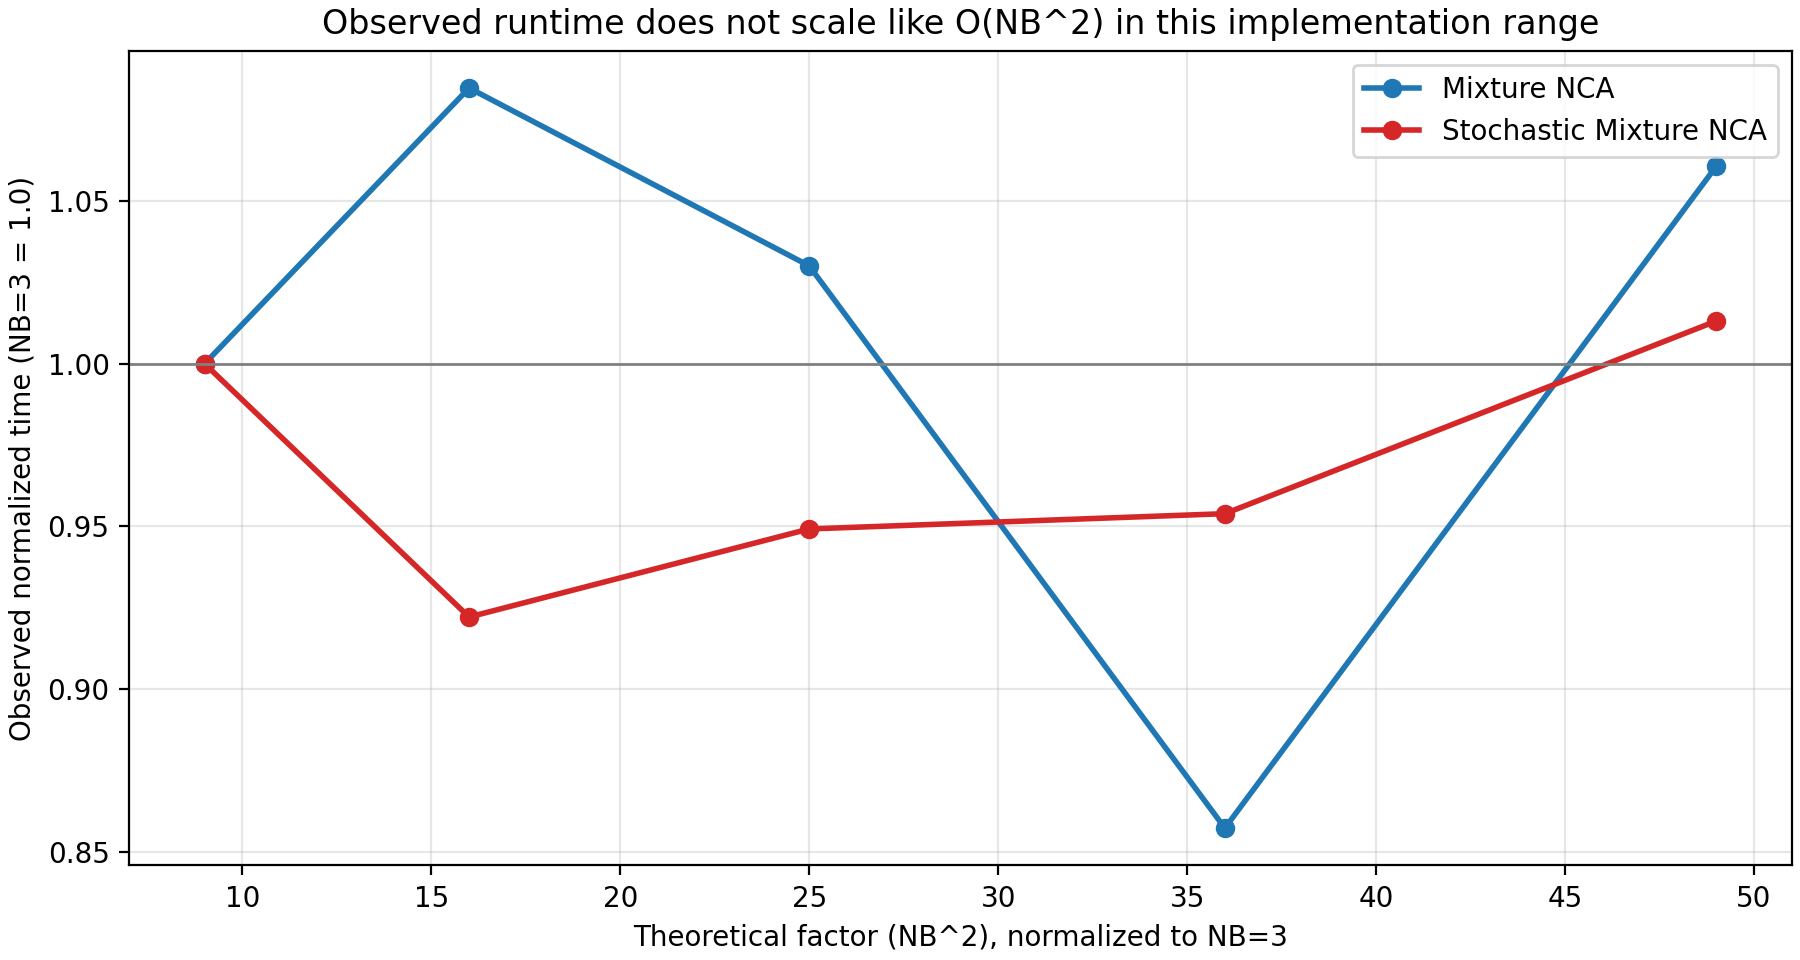
\includegraphics[width=0.85\textwidth]{figs/neighborhood_analysis/nb_sweep_300x100/computational_complexity_normalized_vs_theory.png}
  \caption{Step 3: normalized runtime compared to a theoretical \(NB^2\) scaling. The observed normalized time (relative to \(NB=3\)) stays close to 1.0 and does not increase proportionally to \(NB^2\) in this range.}
  \label{fig:impl:step3:complexity:theory}
\end{figure}

Finally, we analyze how rules are selected over time as a function of neighborhood size, which provides a qualitative explanation for the observed trade-offs and stability differences.
To study how specialization evolves during the dynamics, we measure the entropy of the model's rule-assignment distribution \(p(r \mid x_t)\) at each time step, averaged over space and over sampled simulations.
Low entropy indicates confident (specialized) rule selection, while higher entropy indicates mixed or uncertain rule usage.

\begin{figure}[t]
  \centering
  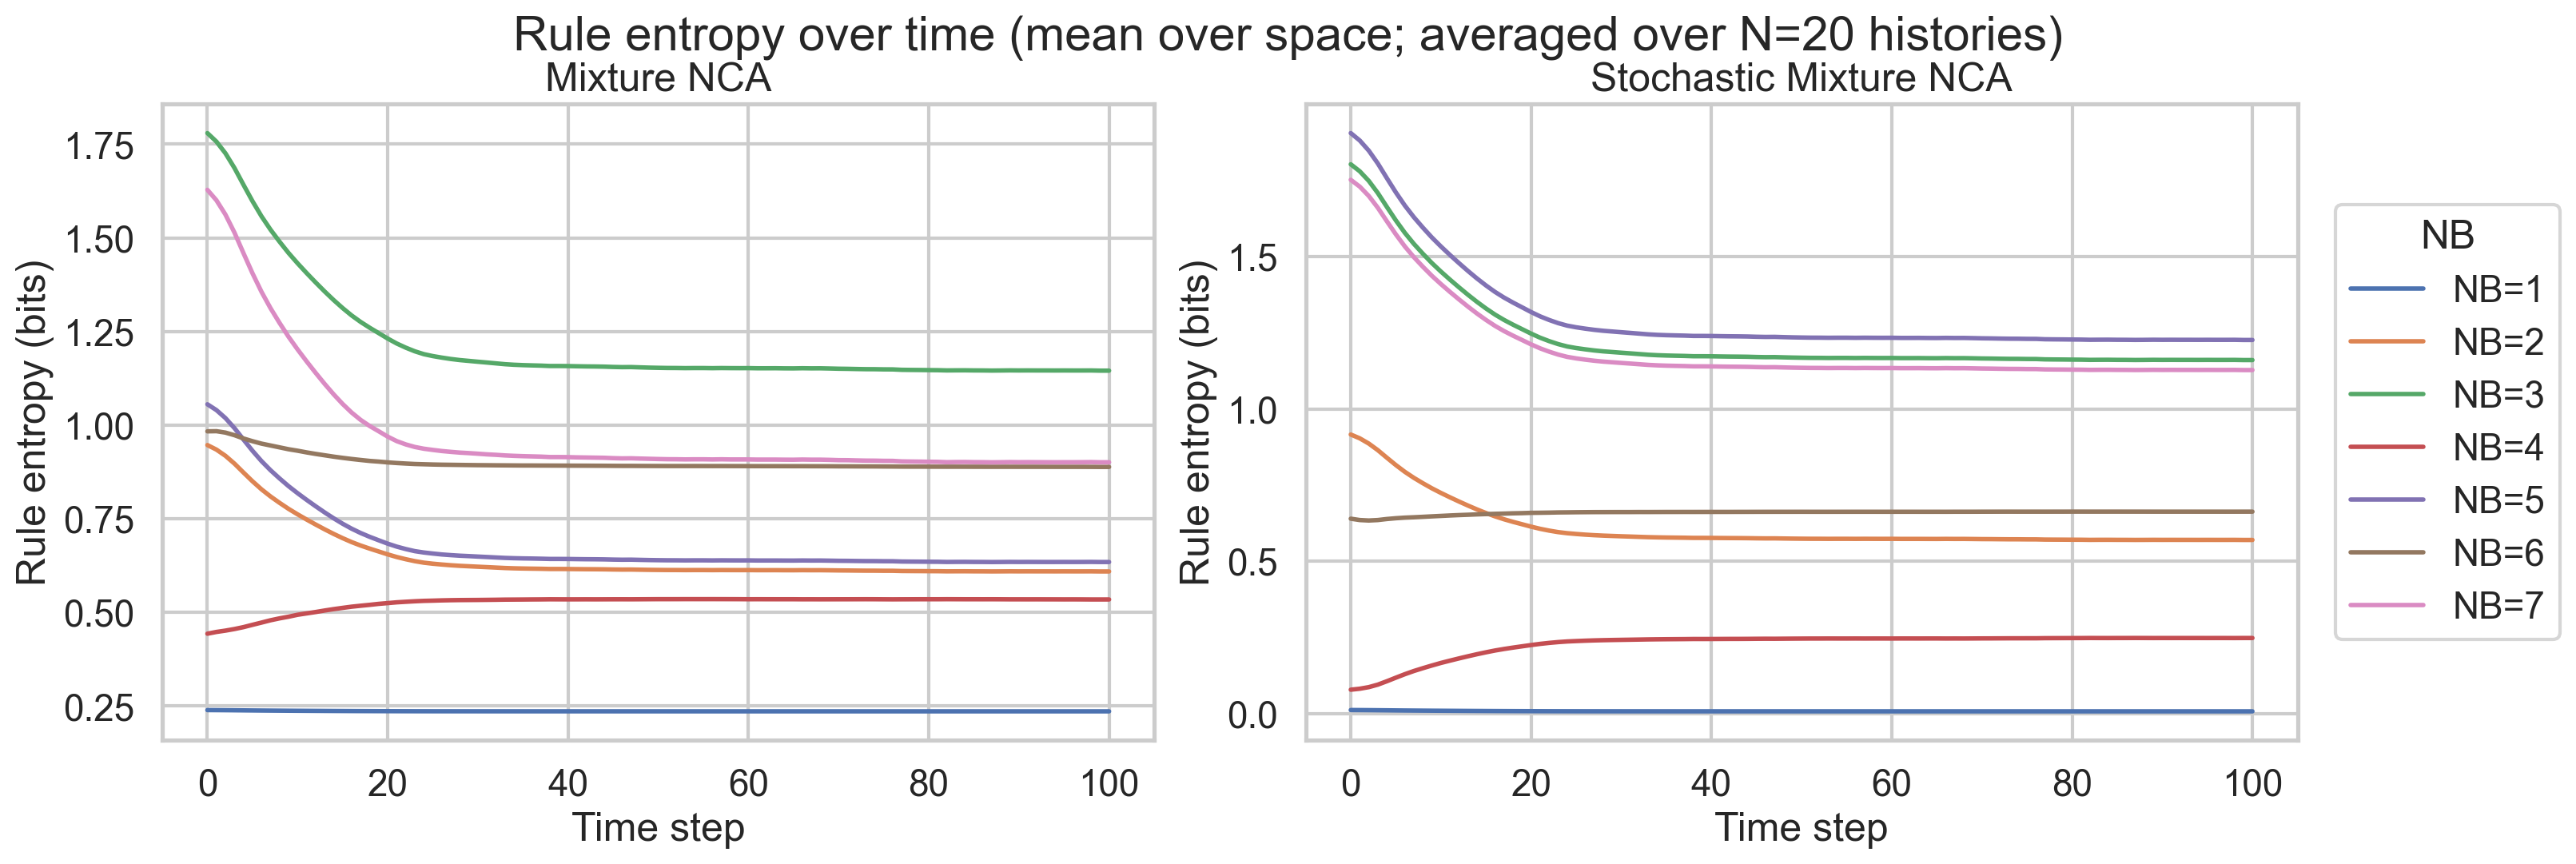
\includegraphics[width=\textwidth]{figs/neighborhood_analysis/nb_sweep_300x100/rule_entropy_over_time.png}
  \caption{Step 3: rule-assignment entropy over time (in bits), averaged over space and across sampled histories (\(N=20\)), for Mixture NCA and Stochastic Mixture NCA on the 300x100 sweep run. Curves correspond to different neighborhood sizes; the temporal profiles highlight how increasing \(NB\) changes the specialization dynamics and can correlate with stability differences.}
  \label{fig:impl:step3:entropy:time}
\end{figure}

\paragraph{Rule specialization summary and interpretation.}
To complement the time-series view, we also summarize rule specialization with three simple indicators:
(i) mean entropy (lower means more confident selection),
(ii) rule diversity (higher means probability mass is spread over more rules),
and (iii) max rule usage (the maximum average probability assigned to a single rule; lower means more balanced usage).
Figure~\ref{fig:impl:step3:rule:summary} reports these indicators and relates them to KL divergence at Step Length \(=100\).

\begin{figure}[t]
  \centering
  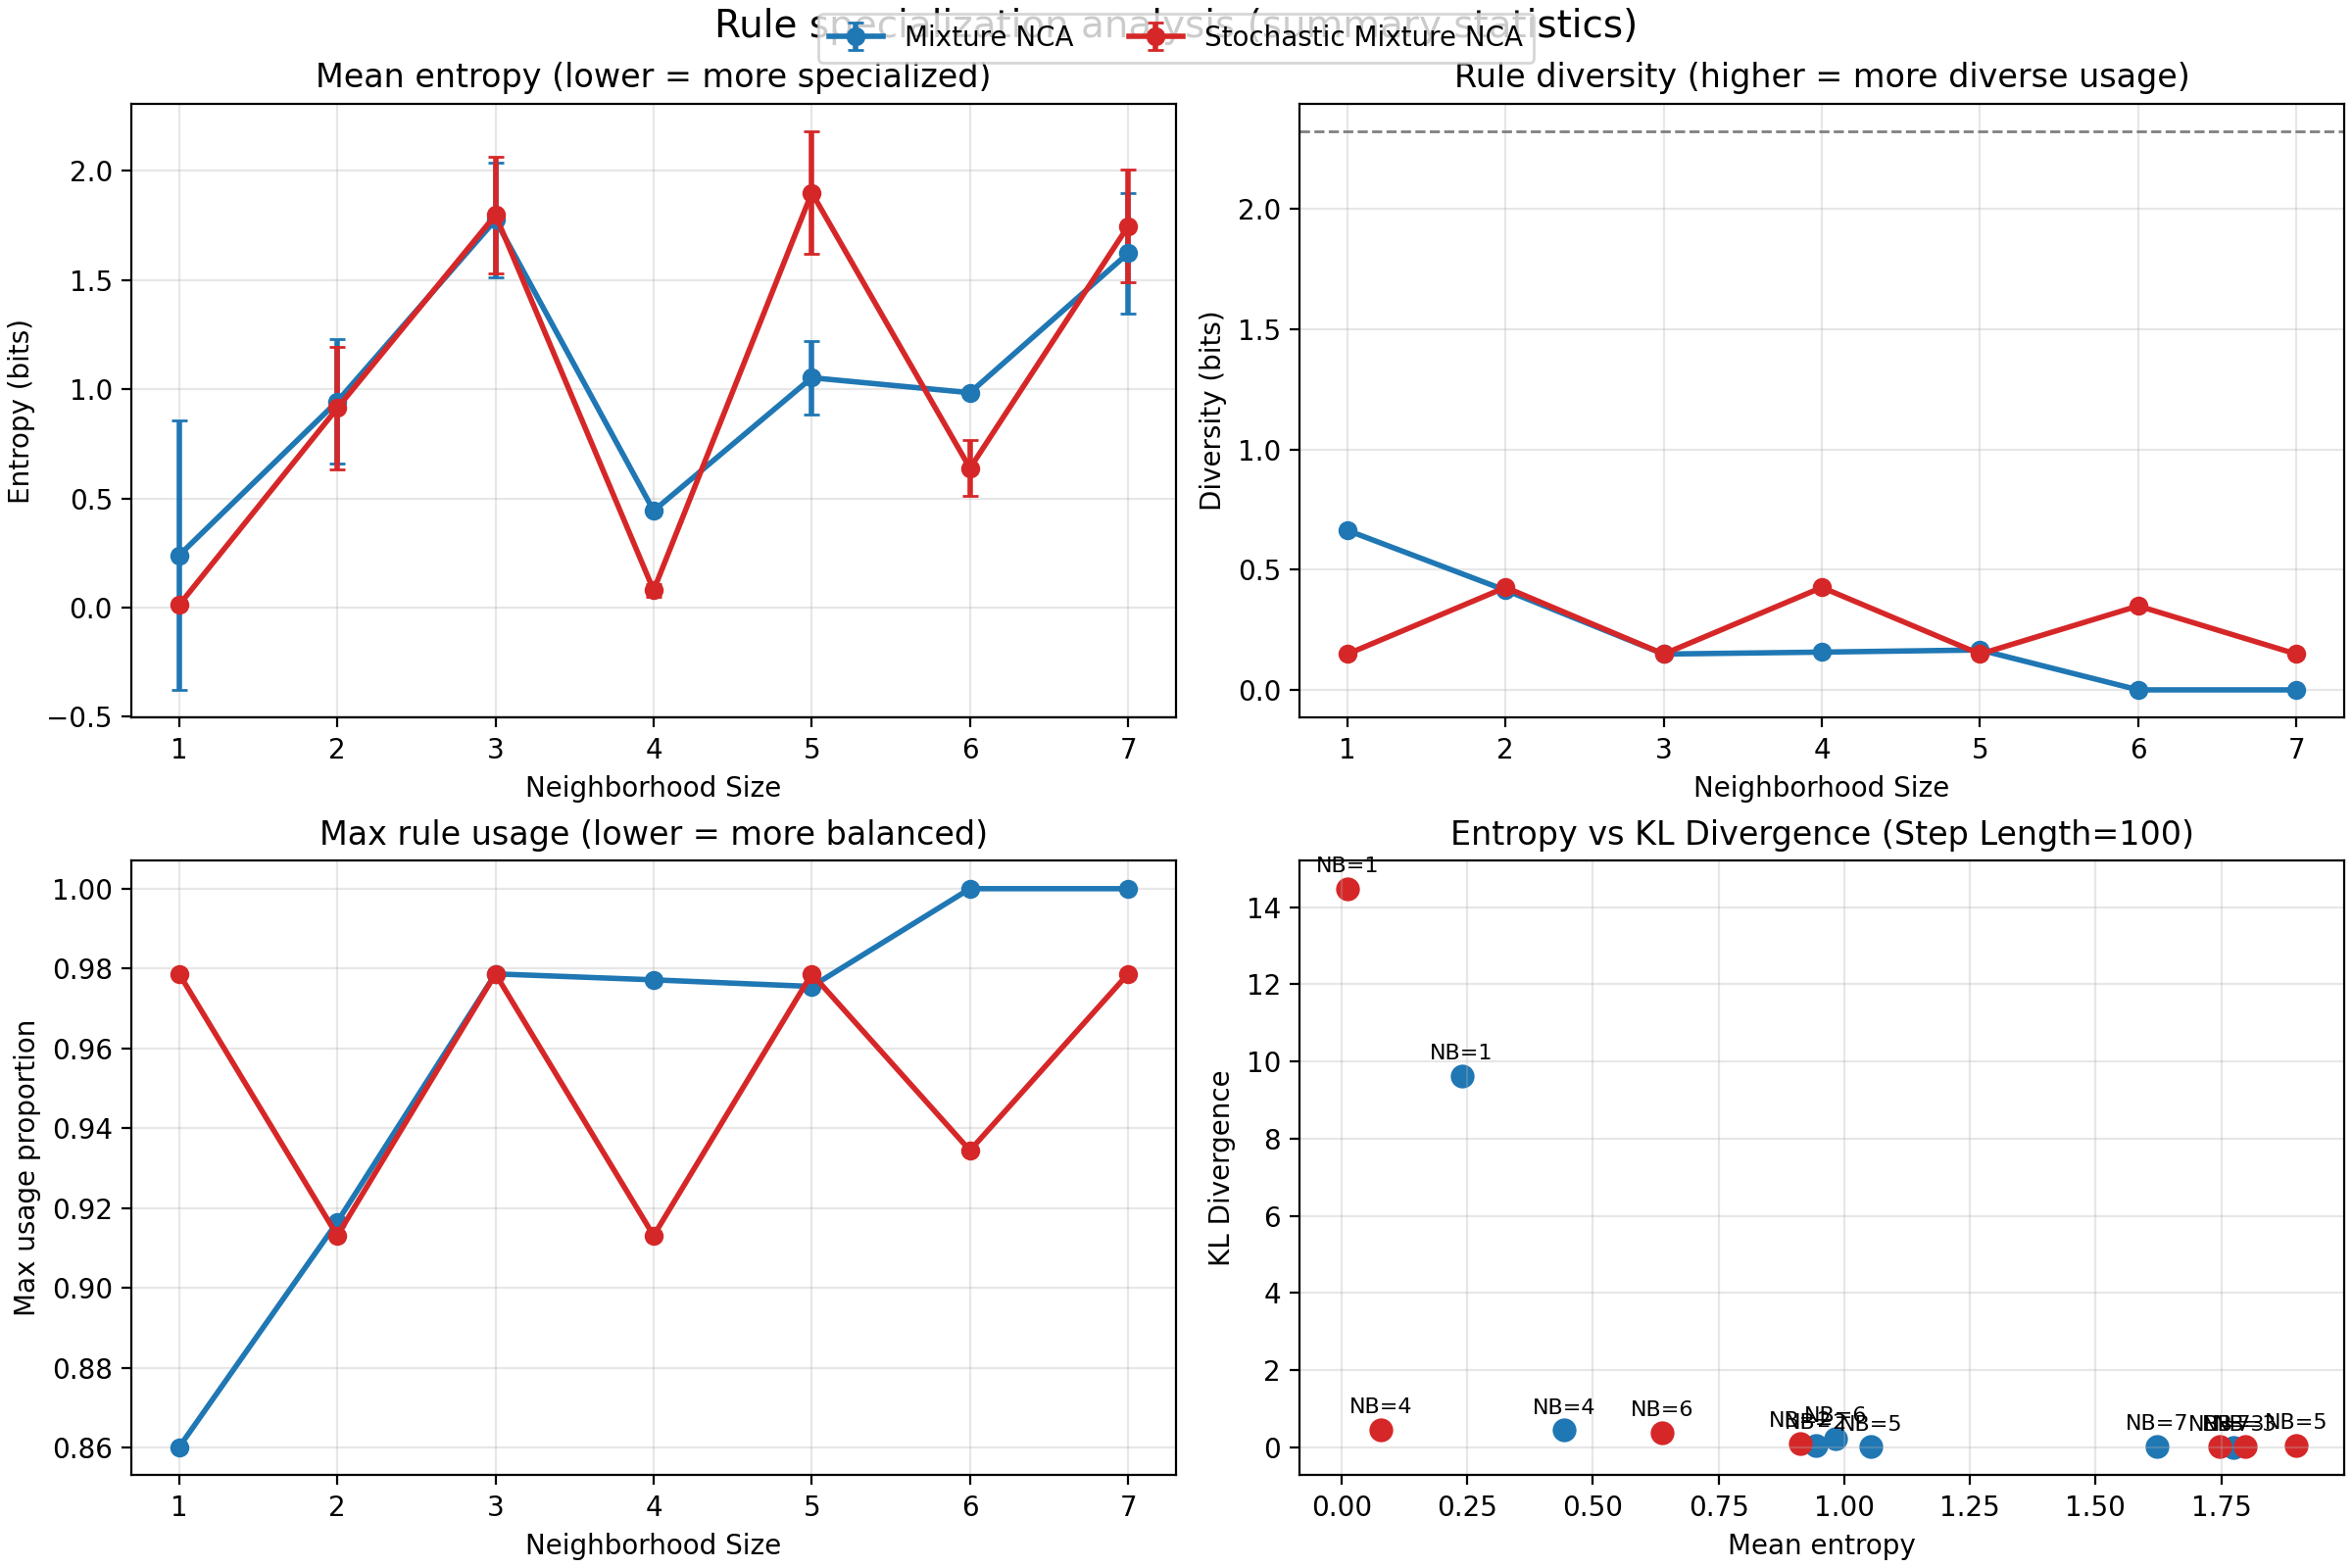
\includegraphics[width=\textwidth]{figs/neighborhood_analysis/nb_sweep_300x100/rule_specialization_summary.png}
  \caption{Step 3: rule specialization summary statistics across neighborhood sizes for Mixture and Stochastic Mixture NCA. The bottom-right panel relates specialization (entropy) to performance (KL divergence) at Step Length \(=100\).}
  \label{fig:impl:step3:rule:summary}
\end{figure}

\paragraph{Rule assignment maps (illustrative examples).}
To make rule selection more intuitive, we visualize the \emph{rule-assignment probability maps} \(p(r \mid x)\) for a single example state.
Each heatmap shows, for each spatial position, how likely the model is to select a given rule.
Figures~\ref{fig:impl:step3:rule:maps:mix} and~\ref{fig:impl:step3:rule:maps:stoch} show examples for selected neighborhood sizes (including small and large \(NB\)).

\begin{figure}[t]
  \centering
  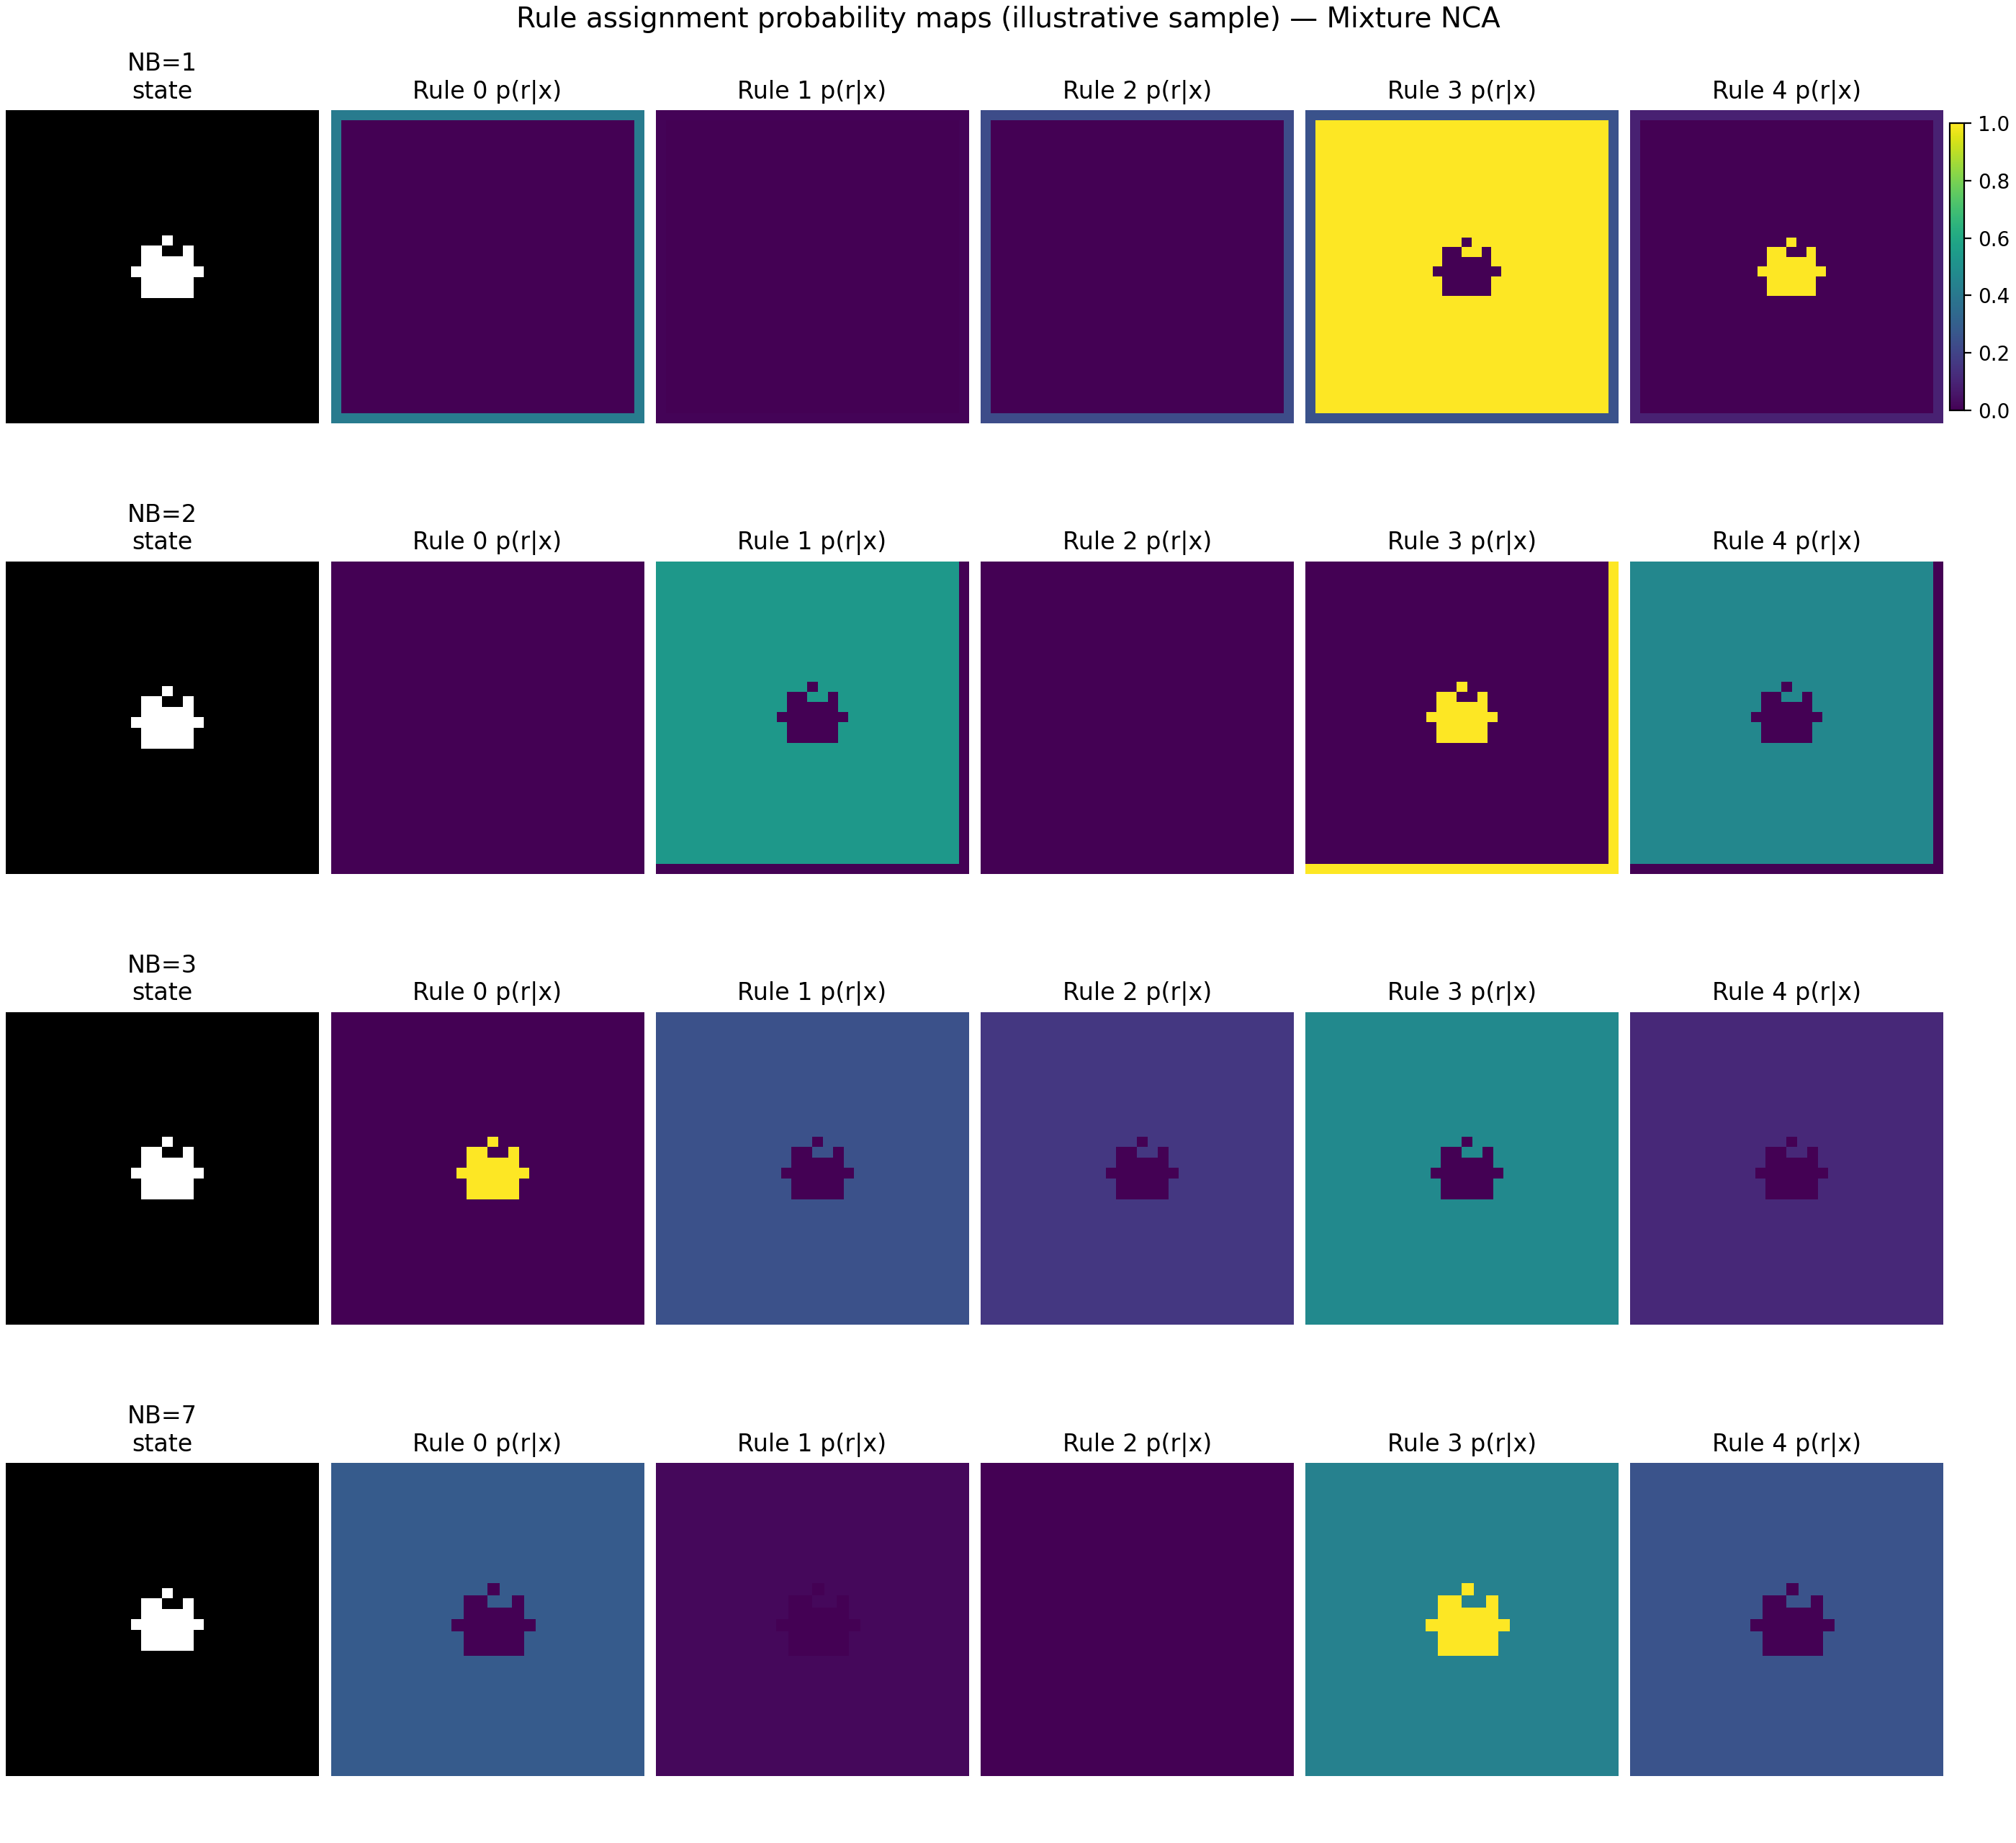
\includegraphics[width=\textwidth]{figs/neighborhood_analysis/nb_sweep_300x100/rule_assignment_maps_mixture.png}
  \caption{Step 3: illustrative rule assignment probability maps for Mixture NCA (one example state). Columns show the input state and the five rule probability maps. Rows correspond to selected neighborhood sizes.}
  \label{fig:impl:step3:rule:maps:mix}
\end{figure}

\begin{figure}[t]
  \centering
  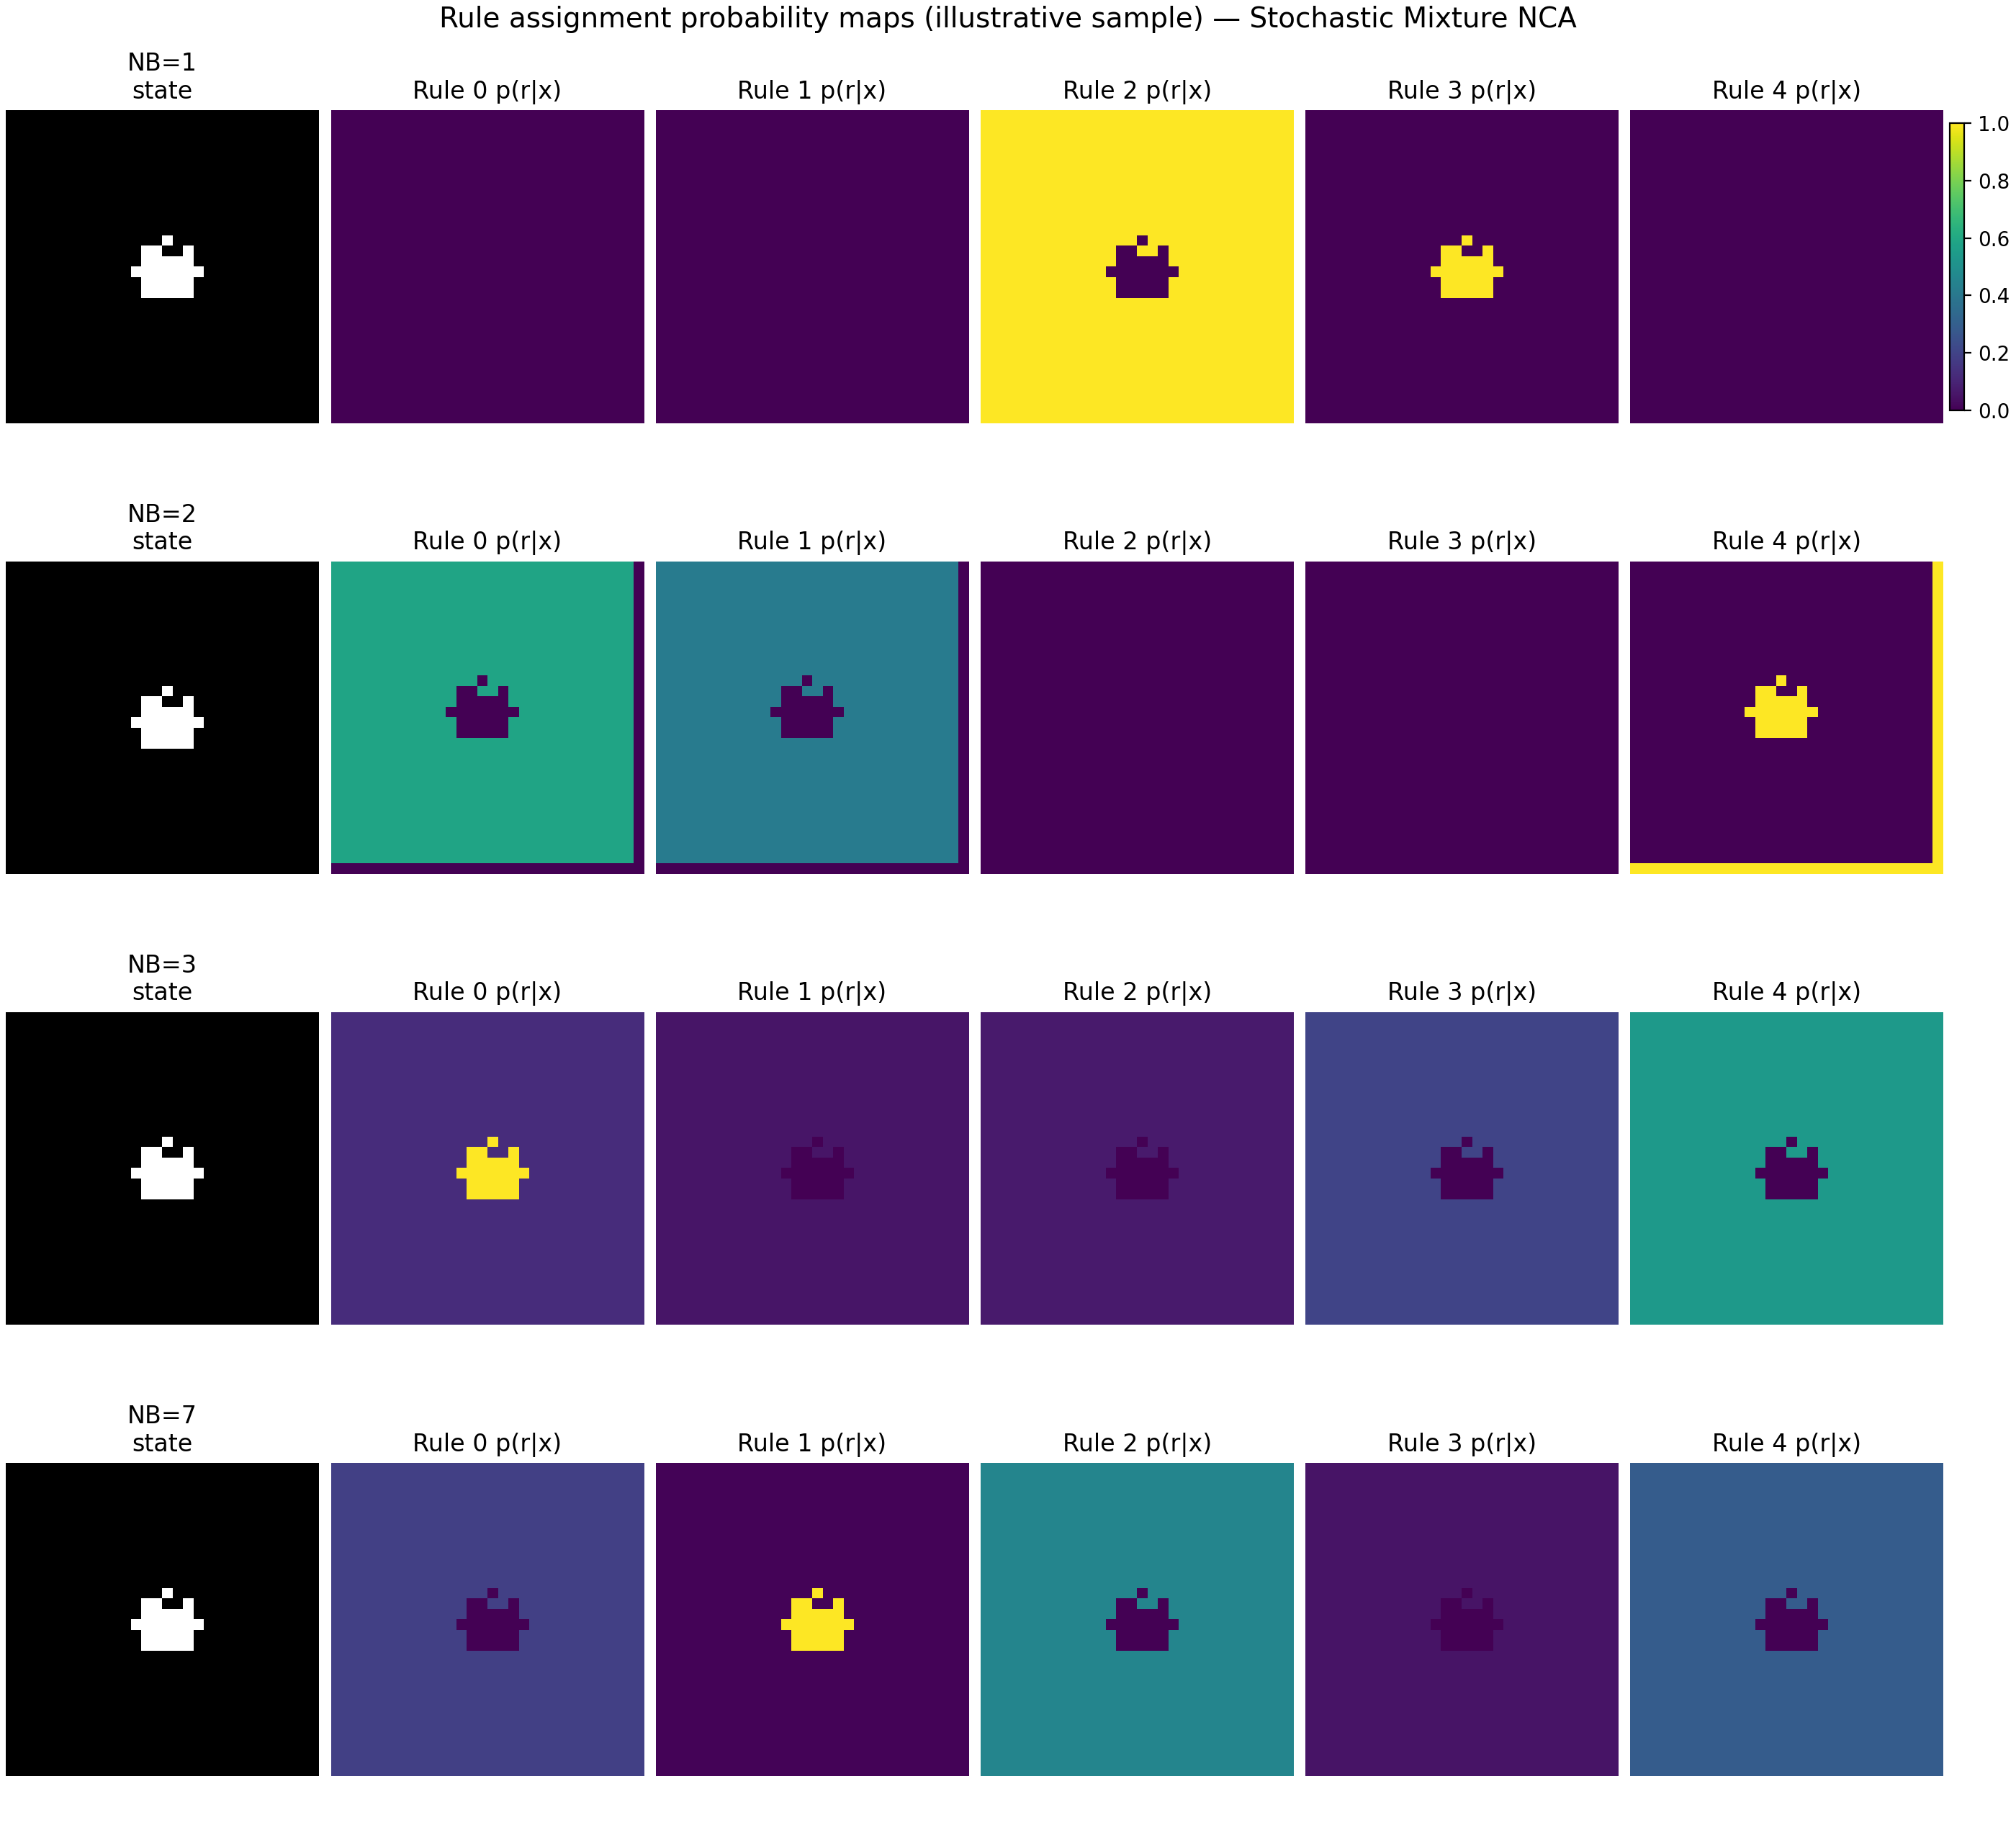
\includegraphics[width=\textwidth]{figs/neighborhood_analysis/nb_sweep_300x100/rule_assignment_maps_stochastic.png}
  \caption{Step 3: illustrative rule assignment probability maps for Stochastic Mixture NCA (one example state). The stochastic variant can exhibit different specialization patterns even when average performance is similar.}
  \label{fig:impl:step3:rule:maps:stoch}
\end{figure}

%----------------------------------------------------------
\subsubsection{Statistical tests (non-parametric)}
\label{sec:impl:step3:stats}
%----------------------------------------------------------

Finally, we add a lightweight statistical check to verify that the observed differences across neighborhood sizes are not explained only by noise.
Because per-simulation metric distributions can be heavy-tailed and not obviously Gaussian, we use non-parametric tests: an overall Kruskal--Wallis test across \(NB\in\{1,\dots,7\}\), followed by post-hoc Mann--Whitney U tests comparing each \(NB\ge2\) against \(NB=1\), with Holm correction within each metric.

% Auto-generated by experiments/generate_step3_stats_table.py
% Statistical tests: Step Length=100, baselines NB=2 and NB=3, Holm correction.
\begin{table}[H]
\centering
\small
\begin{tabulary}{\textwidth}{lLrLL}
\toprule
Model & Metric & Kruskal-Wallis $p$ & Significant vs NB=2 & Significant vs NB=3 \\
\midrule
Mixture~NCA & KL Divergence & $<10^{-4}$ & 3,4,5,6,7 & 4,5,6,7 \\
Mixture~NCA & Chi-Square & $<10^{-4}$ & 3,4,5,6,7 & 4,5,6,7 \\
Mixture~NCA & Categorical MMD & $<10^{-4}$ & 3,4,5,6,7 & 4,5,6 \\
Mixture~NCA & Tumour Size Diff & $<10^{-4}$ & 3,4,5,6,7 & 4,5,6,7 \\
Mixture~NCA & Border Size Diff & $<10^{-4}$ & 3,4,5,6,7 & 4,5,6,7 \\
Mixture~NCA & Spatial Variance Diff & $<10^{-4}$ & 3,4,5,6,7 & 4,5,6,7 \\
Stochastic~Mixture~NCA & KL Divergence & $<10^{-4}$ & 3,4,5,6,7 & 4,5,6,7 \\
Stochastic~Mixture~NCA & Chi-Square & $<10^{-4}$ & 3,4,5,6,7 & 4,5,6,7 \\
Stochastic~Mixture~NCA & Categorical MMD & $<10^{-4}$ & 3,4,5,7 & 4,5,6,7 \\
Stochastic~Mixture~NCA & Tumour Size Diff & $<10^{-4}$ & 3,4,5,7 & 4,5,6,7 \\
Stochastic~Mixture~NCA & Border Size Diff & $<10^{-4}$ & 4,5,6,7 & 4,5,6,7 \\
Stochastic~Mixture~NCA & Spatial Variance Diff & $<10^{-4}$ & 3,4,5,6,7 & 4,5,7 \\
\bottomrule
\end{tabulary}
\caption{Non-parametric statistical tests across neighbourhood sizes for Step Length $=100$. \textbf{Legend:} Model = Mixture NCA or Stochastic Mixture NCA; Metric = one of the six metrics; Kruskal-Wallis $p$ over $NB\in\{1,\dots,7\}$; last two columns = list of $NB$ that differ significantly from baseline $NB=2$ (post-hoc Mann-Whitney U, Holm correction) and from baseline $NB=3$.}
\label{tab:impl:step3:stats}
\end{table}


%-------------------------------------------------------------------
\chapter{Interactive platform with Streamlit}
\label{c:streamlit}
%-------------------------------------------------------------------

To make the results of the Mixture NCA experiments easy to explore and to support a direct visual comparison between model predictions and ground truth, an interactive web application was built using Streamlit.
This chapter outlines the motivations for this choice, what the platform is and what it is used for, how it was developed, its main functionalities (with screenshots), and why the predictions shown in the interface do not align fully with the true ground truth.
It also explains why the dashboard is set up to display only the results of the latest curriculum learning experiment.

%----------------------------------------------------------
\section{Motivations and role of Streamlit}
%----------------------------------------------------------

Streamlit is an open-source framework for building web interfaces for data science and machine learning applications from Python scripts, without writing HTML, CSS or JavaScript.
Its adoption in this work was driven by practical needs.
First, the experiments described in Chapter~\ref{c:implementation} produce a large amount of data: trained checkpoints for different neighborhood sizes, aggregated biological metrics, and simulation trajectories that are naturally explored in an interactive way.
Making these results available through a self-contained application allows users to pick an experiment, load a checkpoint, run a rollout and compare the model output with the simulator trajectory frame by frame, without re-running command-line scripts or opening notebooks each time.
Second, Streamlit makes it possible to obtain a usable interface quickly: widgets such as sliders, select boxes, tabs and expanders, as well as column layouts, are built in, and integration with libraries like Plotly for charts and PyTorch for loading models is straightforward.
Finally, the application can be run locally and, if desired, deployed on platforms such as Streamlit Cloud or an internal server, keeping a single codebase for both analysis and demonstration.

In our setting, the platform serves a dual purpose: it is a tool for \emph{testing and inspecting} trained models (choosing the experiment, model type and initial state, and viewing the rollout alongside ground truth), and at the same time a \emph{dashboard} that aggregates metrics and experiment configuration by neighborhood size and model type, in line with the folder structure produced by the curriculum learning pipeline described in Chapter~\ref{c:implementation}.

%----------------------------------------------------------
\section{Development and architecture}
%----------------------------------------------------------

The application is organised around a small set of components: a main entry point that handles page configuration and navigation, a layer responsible for loading trained models and running rollouts, and a dashboard layer that discovers and aggregates experiment outputs.

The main component sets the page layout (wide, with an expanded sidebar), keeps session state for rollout frames and for a cache of loaded models, and provides navigation between two views via a sidebar radio control: ``Model test'' and ``Experiments dashboard''.
By default, the application reads from the results directory produced by the curriculum learning pipeline.
Inside that directory it looks for subfolders named by neighborhood size (e.g.\ \texttt{NB\_2}, \texttt{NB\_3}, \texttt{NB\_5}) and uses them as the list of available experiments.

Model loading and rollout execution are handled by a dedicated module.
For each experiment folder, the application looks for final checkpoints (excluding intermediate phase checkpoints), infers the neighborhood size from the folder name, and instantiates the corresponding Mixture NCA or Stochastic Mixture NCA with the same architecture as in training.
The rollout is run from an initial state given as a grid of cell types (e.g.\ taken from the same history dataset used in training), with a configurable number of steps (up to 500) and, for the stochastic model, an optional seed for reproducibility.
The resulting frames are converted to RGBA images for display (mapping cell types to the colours defined in the tissue model) and shown side by side with ground-truth frames when the latter are available.

The dashboard component scans the results directory, reads for each neighborhood-sized subfolder the stored configuration and curriculum metadata and the computed biological metrics (per step length and model type), and builds a structured representation of each experiment.
Metrics from all experiments can be aggregated into a single table or visualised with interactive charts (e.g.\ KL divergence, Chi-Square, Categorical MMD, tumor size difference, border size difference, spatial variance difference).

%----------------------------------------------------------
\section{Functionality and screens}
%----------------------------------------------------------

\paragraph{Model test.}
On the ``Model test'' page the user selects in the sidebar the results folder, the experiment (neighborhood size), the model type (Mixture NCA or Stochastic Mixture NCA), and optionally the history dataset and the simulation and initial-frame indices.
A ``Simulate'' button starts the rollout; when it finishes, a confirmation message appears (e.g.\ ``Simulation completed: 500 frames'') and a ``Frame'' slider allows stepping through time.
For each selected step, two images are shown side by side: on the left the ground-truth frame from the simulator, on the right the frame predicted by the model at that step.
Grids are rendered with nearest-neighbour interpolation (pixelated) so that discrete cells remain visually clear.

Figure~\ref{fig:streamlit:model_test_step0} shows the interface at the initial step (step 0): the initial state is the same for both columns (same seed or history), but even at this frame small differences can appear due to how the model represents and evolves the state.
Figures~\ref{fig:streamlit:model_test_step177} and~\ref{fig:streamlit:model_test_step499} show the same comparison at steps 177 and 499.
As time advances, the shape and distribution of cell types (in particular the red cells, typically differentiated or in transition) in the prediction can diverge from the real trajectory: the predicted structure often looks more fragmented, with red pixels more spread inside the tissue, whereas in the ground truth red cells tend to concentrate along the boundaries and in more defined regions.
This kind of mismatch is exactly what is discussed in Section~\ref{sec:streamlit:alignment} and has already been analysed from a methodological standpoint in \cref{sec:impl:curriculum:limitations}.

\begin{figure}[H]
  \centering
  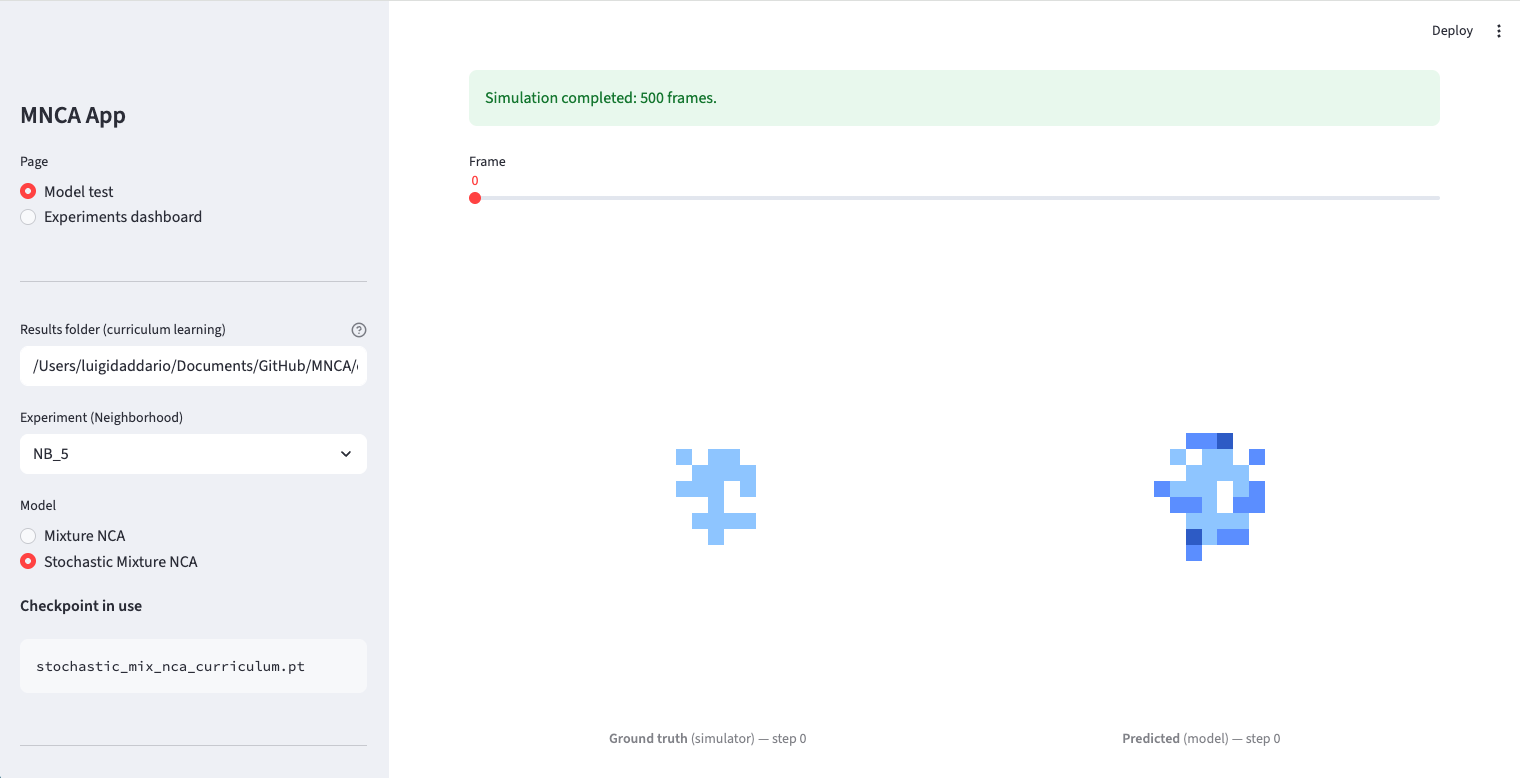
\includegraphics[width=0.95\textwidth]{figs/streamlit/streamlit_model_test_step0.png}
  \caption{``Model test'' page of the MNCA platform: comparison of ground truth (left) and prediction (right) at step 0. Sidebar: experiment (e.g.\ neighborhood 5), model (Stochastic Mixture NCA) and checkpoint in use.}
  \label{fig:streamlit:model_test_step0}
\end{figure}

\begin{figure}[H]
  \centering
  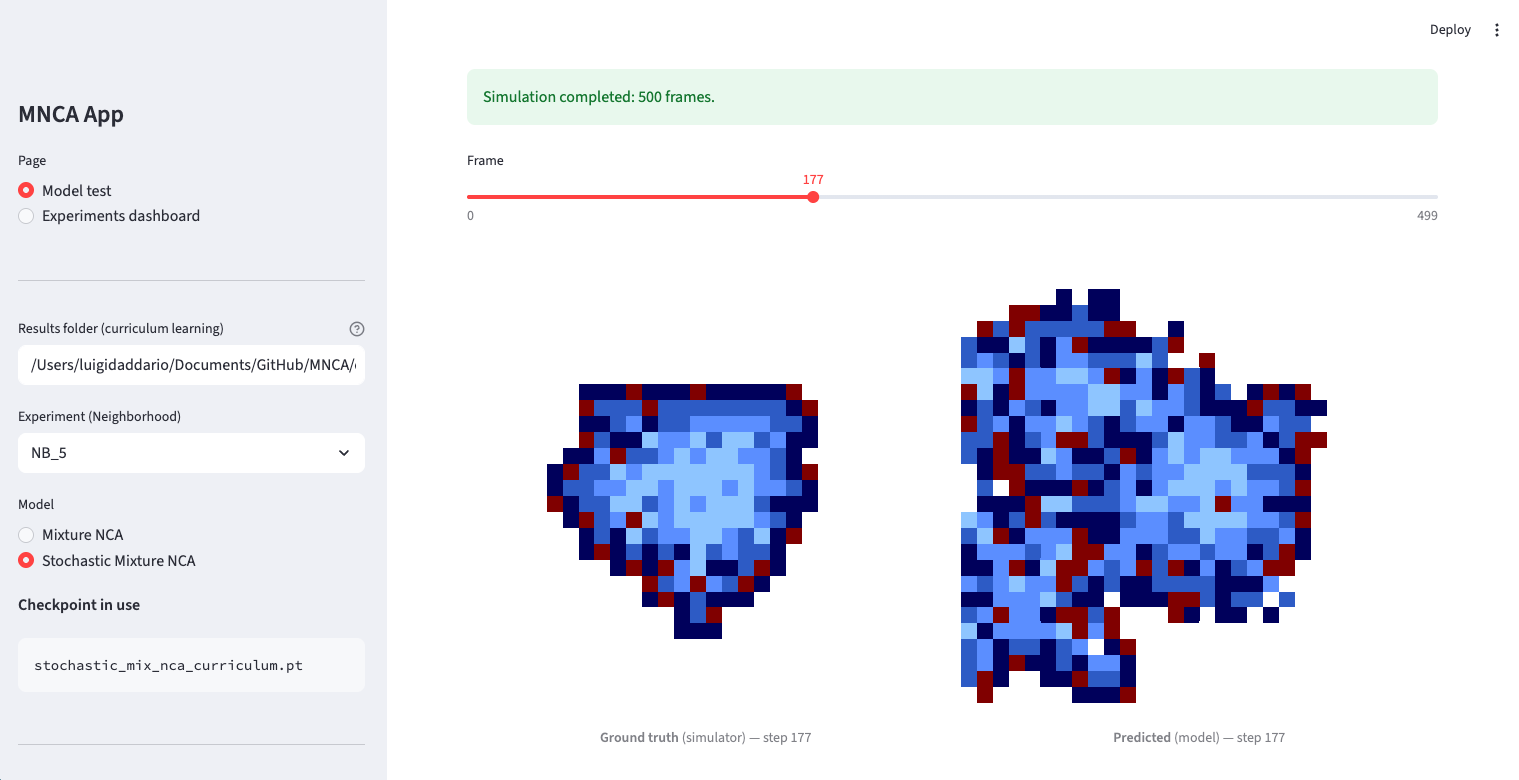
\includegraphics[width=0.95\textwidth]{figs/streamlit/streamlit_model_test_step177.png}
  \caption{Same Model test session at step 177. The prediction (right) begins to show a slightly different cell-type distribution and morphology compared to the ground truth (left).}
  \label{fig:streamlit:model_test_step177}
\end{figure}

\begin{figure}[H]
  \centering
  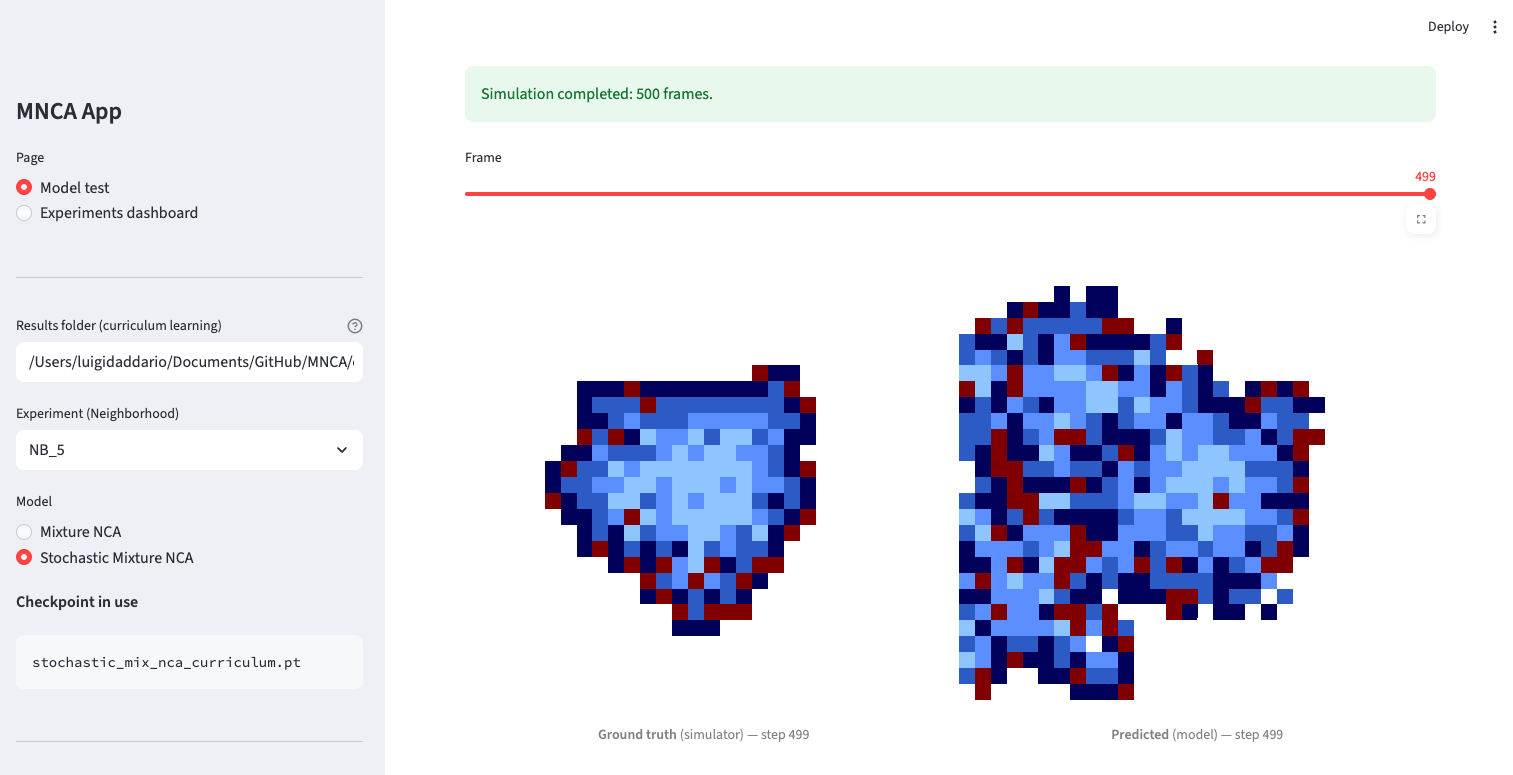
\includegraphics[width=0.95\textwidth]{figs/streamlit/streamlit_model_test_step499.png}
  \caption{Comparison at step 499 (end of rollout). The divergence between prediction and ground truth is more pronounced: less compact structure and greater spread of red pixels in the prediction.}
  \label{fig:streamlit:model_test_step499}
\end{figure}

\paragraph{Experiments dashboard.}
The ``Experiments dashboard'' page provides an aggregated view by neighborhood size and model type.
In the sidebar the user can set the results directory; the application reports how many experiment subfolders it found.
The main area has three tabs: an experiment summary (per neighborhood), a full metrics table, and overview charts.

In the summary tab, each experiment is shown in an expandable block with the neighborhood identifier and size.
Inside are the configuration (training parameters, curriculum), the list of saved checkpoints (final results only, no phase checkpoints), and the biological metrics both as a table and as charts (metrics vs.\ step length for that neighborhood).
Figure~\ref{fig:streamlit:dashboard_summary} shows an example with one neighborhood expanded and the curriculum section visible (time length, epochs, learning rate per phase).

In the metrics tab, all metrics from the discovered experiments are merged into a single table (Figure~\ref{fig:streamlit:dashboard_metrics}), with columns for model type, KL Divergence, Chi-Square, Categorical MMD, Tumor Size Diff, and so on, with standard deviations when available.
This allows a quick comparison across neighborhood sizes and between Mixture NCA and Stochastic Mixture NCA.
The overview charts tab displays the same data graphically (via Plotly), with one subplot per metric.

\begin{figure}[H]
  \centering
  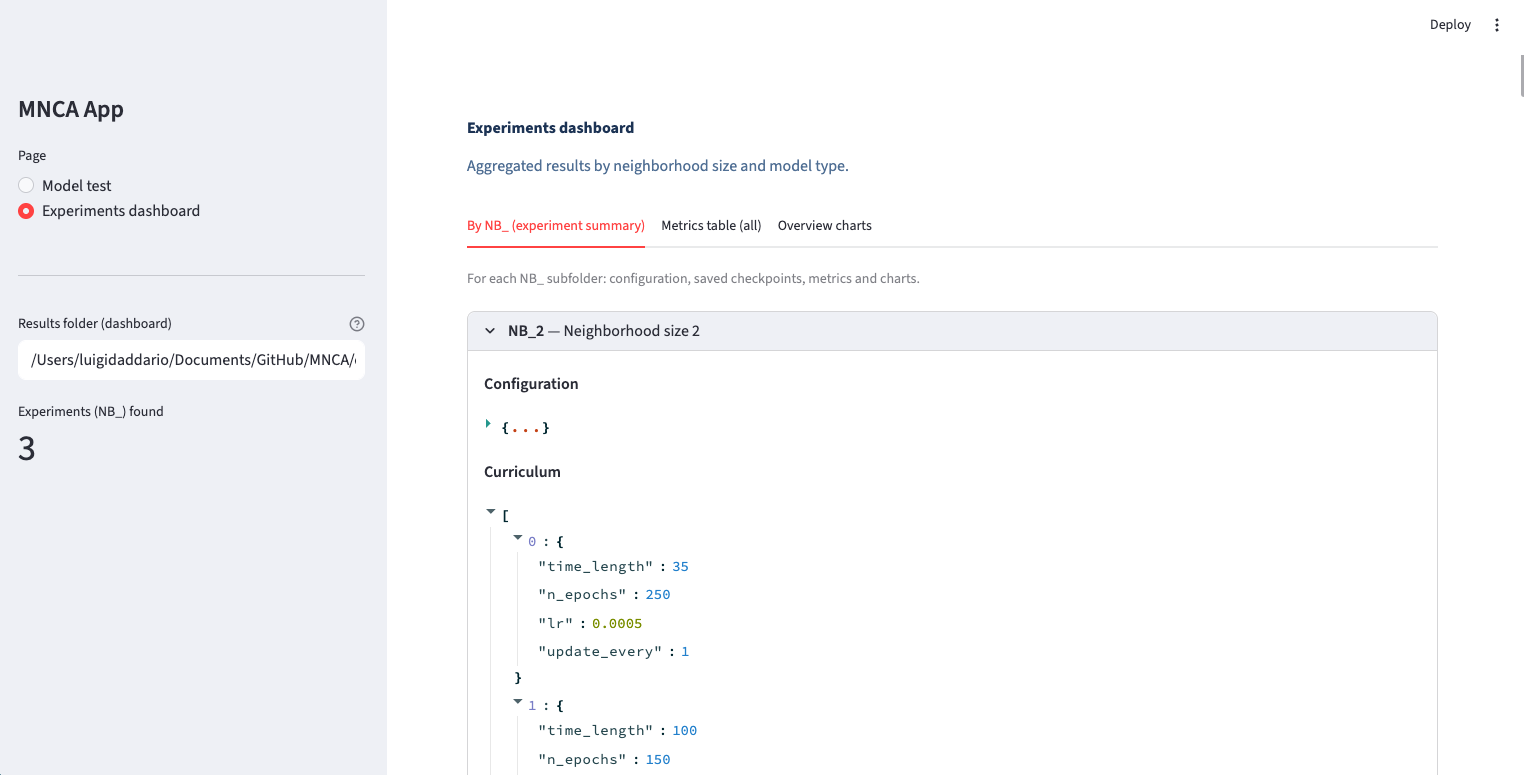
\includegraphics[width=0.95\textwidth]{figs/streamlit/streamlit_dashboard_summary.png}
  \caption{Experiments dashboard, summary tab: detail for one neighborhood with configuration and curriculum (time length, epochs, learning rate per phase).}
  \label{fig:streamlit:dashboard_summary}
\end{figure}

\begin{figure}[H]
  \centering
  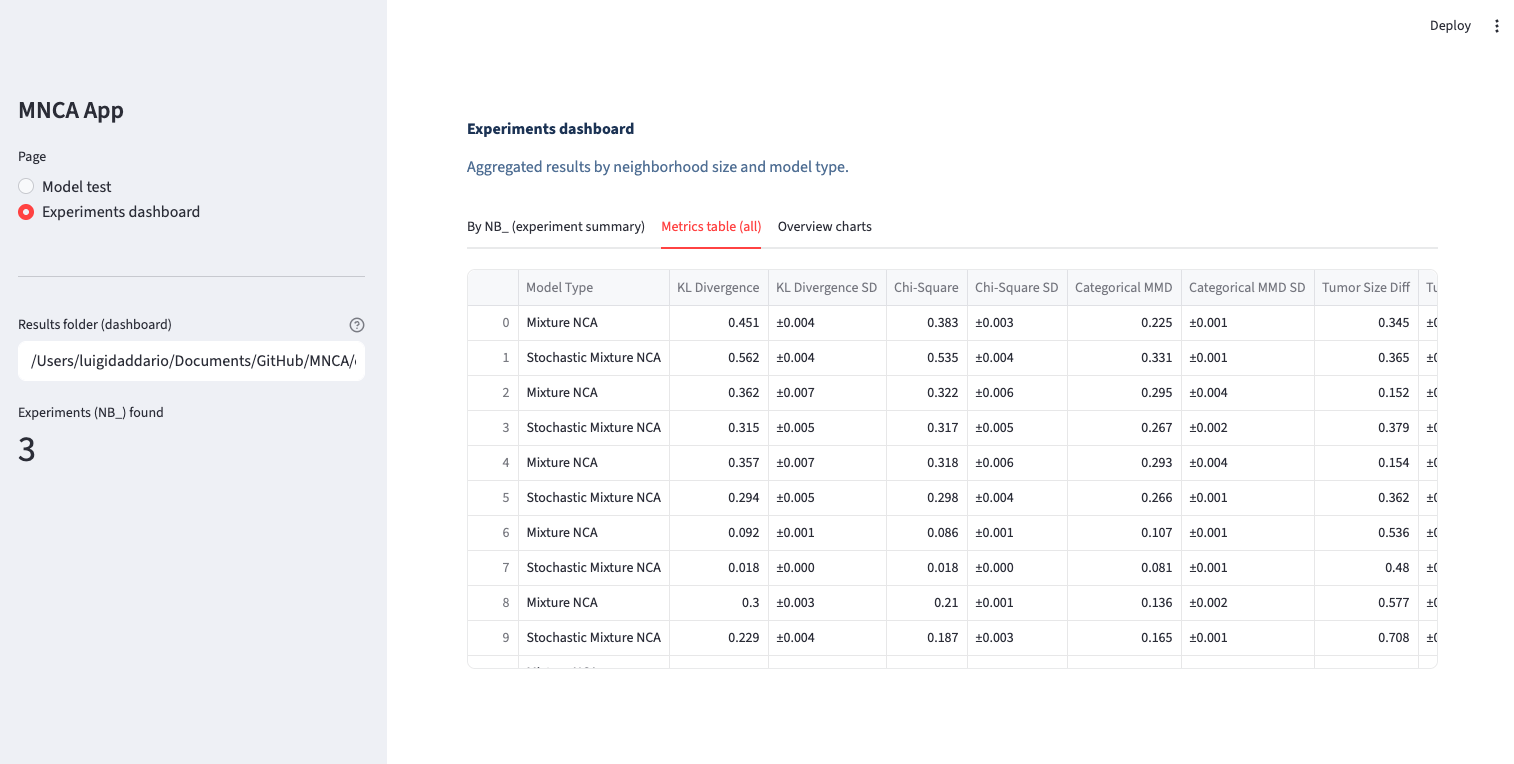
\includegraphics[width=0.95\textwidth]{figs/streamlit/streamlit_dashboard_metrics.png}
  \caption{Experiments dashboard, metrics tab: aggregated table of metrics (KL Divergence, Chi-Square, Categorical MMD, Tumor Size Diff, etc.) for all experiments and model types.}
  \label{fig:streamlit:dashboard_metrics}
\end{figure}

%----------------------------------------------------------
\section{Why the prediction does not align with ground truth}
\label{sec:streamlit:alignment}
%----------------------------------------------------------

When viewing the frame-by-frame comparison on the Model test page, it is clear that the trajectory generated by the model does not match the simulator trajectory, especially at later steps.
This misalignment is not a flaw of the interface but reflects inherent limitations in how the models are trained and evaluated, already discussed in \cref{sec:impl:curriculum:limitations}; here we give a concise, user-oriented reading of the same phenomena.

During training, teacher forcing is used: at each step the model receives the \emph{true} state from the training history, so errors do not accumulate and the loss can stay low.
At test time, by contrast, free rollouts are run: the model receives only its own previous output as input.
A small error at step 10 is then fed into step 11 and so on; after hundreds of steps the trajectory can drift noticeably from the ground truth even if the model has learned the local dynamics well.
In other words, the loss that is optimised is a step-by-step mean squared error over the training window; it encourages correct prediction of the next state given the current one, but does not directly reward the fact that an entire free trajectory matches a single simulator realisation.
It is therefore possible to have a model with low loss and at the same time clear drift when it is run autonomously.

For the Stochastic Mixture NCA there is an additional factor: at each step a rule is sampled, so different runs with different seeds produce different trajectories.
The ground truth we compare against is only one possible realisation of the stochastic simulator; part of the ``difference'' we see is thus natural variability between realisations, not only model error.
Even so, the figures often show an over-abundance of differentiated (red) cells and a less compact structure in the prediction, indicating that the model has not yet perfectly learned the long-horizon dynamics.

Finally, the last phase of the curriculum uses 500-step windows but with fewer epochs and a reduced learning rate; training may stop before the model has fully stabilised behaviour over the full horizon, contributing to the gap observed at the final steps.
The Streamlit platform makes this phenomenon directly visible and interpretable without re-running evaluation scripts.

%----------------------------------------------------------
\section{Choice of results shown in the dashboard}
%----------------------------------------------------------

The application is configured to read results from a single root directory, the one produced by the curriculum learning pipeline.
Within it, all subfolders corresponding to neighborhood sizes are detected; the dashboard then aggregates whatever is present in that directory (configuration, checkpoints, metrics).

In this thesis we have chosen to use the platform with the results of the \emph{latest} curriculum experiment, i.e.\ the one whose parameters and metrics are described in Chapter~\ref{c:implementation} and discussed in the results.
In this way the dashboard does not mix runs from different campaigns (e.g.\ earlier neighborhood sweeps or experiments with different history lengths), but reflects a single coherent set of runs: the same training conditions, the same history dataset and the same curriculum phases.
A user opening the application therefore sees exactly the results that underpin the experimental part of the thesis, and can inspect for each neighborhood the configuration, saved checkpoints and biological metrics, and test the models interactively by loading initial states from the same histories used in training.
If in the future other experiments were to be included, it would suffice to point the results folder to another path or to combine several directories into one; the application logic would remain the same and would continue to discover all neighborhood-sized subfolders in the configured directory.

%-------------------------------------------------------------------
\chapter{Results}
\label{c:results}
%-------------------------------------------------------------------

This chapter summarises the main results of the thesis. It focuses on what we learned about Mixture Neural Cellular Automata (MNCA) for modelling tissue-like dynamics, and in particular on the role of the spatial neighbourhood size (\(NB\)). Experimental setups and implementation details are described in \cref{c:implementation}; here we concentrate on the figures, tables, and their interpretation.

%-------------------------------------------------------------------
\section{NB size effects in synthetic tissue models}
\label{sec:results:neighborhood}
%-------------------------------------------------------------------

Across the synthetic experiments, the evidence consistently indicates that \textbf{neighbourhood size is not a marginal hyperparameter}: it changes stability, long-horizon behaviour, and the trade-off between matching global statistics and reproducing spatial structure.
With minimal context (\(NB=1\), each cell sees only itself) the model is inadequate for the task; the analysis therefore focuses on \(NB \ge 2\).
In the controlled neighbourhood sweep (Step~3, \cref{sec:impl:step3:results}), \textbf{Kruskal-Wallis tests return \(p < 10^{-4}\)} across all metrics for both Mixture NCA and Stochastic Mixture NCA, and post-hoc comparisons (against baselines \(NB=2\) and \(NB=3\)) show that multiple neighbourhood sizes differ significantly from each other.

The main finding is that \textbf{once \(NB \ge 2\), performance does not improve monotonically with neighbourhood size}.
Different neighbourhood sizes lead to different compromises, and the ``best'' setting depends on (i) which metric is prioritised and (ii) the rollout horizon used for evaluation.

\subsection{Step 3: detailed trends across neighbourhood sizes}
\label{sec:results:step3}
%-------------------------------------------------------------------

In Step 3 we trained Mixture NCA and Stochastic Mixture NCA on \textbf{300 ground-truth histories of length 100}, one model per neighbourhood size \(NB \in \{1,\dots,7\}\), and evaluated them at three rollout horizons (Step Length \(=25, 50, 100\)).
For each configuration (model, \(NB\), step length) we computed six biological metrics on the final generated state (KL divergence, Chi-square, categorical MMD, tumour size difference, border size difference, spatial variance difference), averaged them across runs, and also inspected their per-simulation distributions.

Figure~\ref{fig:impl:step3:dashboard} reports the mean and variability of all six metrics across neighbourhood sizes.
The main qualitative pattern is consistent across metrics: \(NB=1\) is systematically inadequate, while moving to \(NB\ge2\) yields a sharp performance improvement.
Beyond this first jump, increasing \(NB\) produces a non-monotonic trade-off between matching global distributions (e.g., KL divergence) and matching spatial structure (e.g., tumour size and border properties).

\begin{figure}[H]
  \centering
  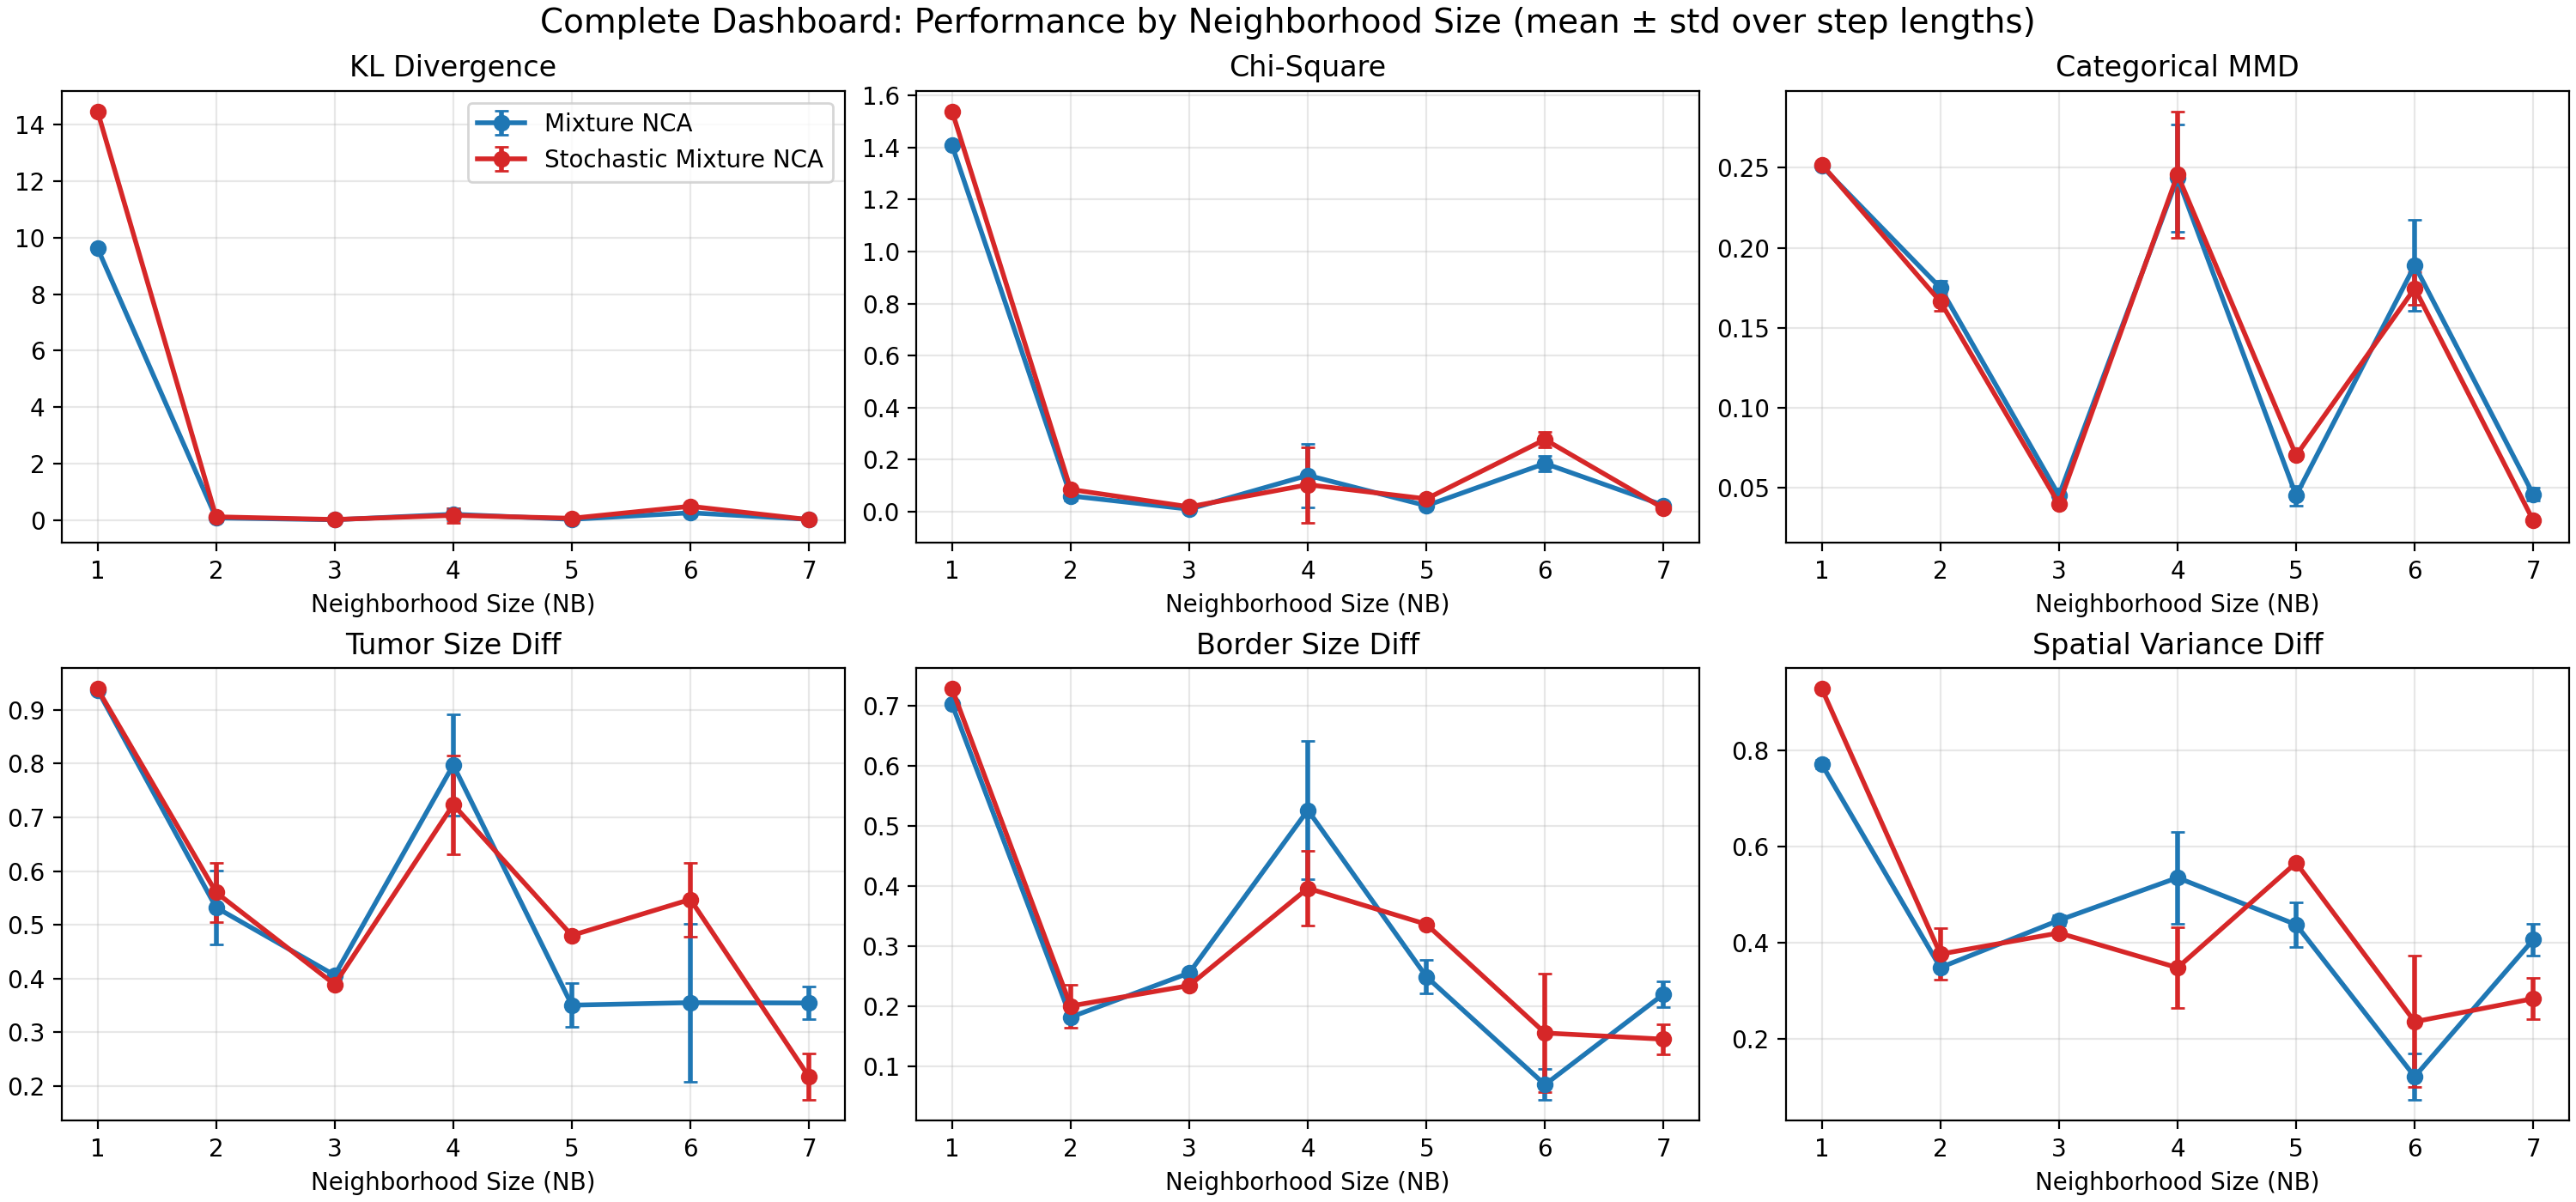
\includegraphics[width=\textwidth]{figs/neighborhood_analysis/nb_sweep_300x100/metrics_dashboard_full.png}
  \caption{Step 3: complete dashboard for the neighbourhood sweep. \textbf{Legend:} each panel is one of the six metrics (KL divergence, Chi-square, categorical MMD~\cite{gretton2012mmd}, tumour size difference, border size difference, spatial variance difference); abscissa = neighbourhood size \(NB\); ordinate = metric value (lower is better); mean and standard deviation over step-length conditions; series distinguish Mixture NCA vs.\ Stochastic Mixture NCA.}
  \label{fig:impl:step3:dashboard}
\end{figure}

\newpage
\vspace{-0.5em}
\subsubsection{Distributional agreement and per-simulation variability}
\label{sec:results:step3:kl}
\vspace{-0.8em}
KL divergence captures how well the global composition of cell types in the generated final state matches the empirical distribution from the dataset.
Across all step lengths, \(NB=1\) yields very large KL values, indicating a strong mismatch in global composition.
For \(NB\ge2\), both models reach low KL on average, but the best neighbourhood can depend on the evaluation horizon and on whether rule selection is deterministic or stochastic.
\vspace{-0.4em}
To interpret robustness, we inspect \emph{per-simulation} distributions of the metrics using violin plots.
Compared to mean-only summaries, violins reveal heavy tails and outliers: these correspond to runs that converge to qualitatively wrong outcomes (failure modes), even when the median performance is competitive.
\vspace{-0.6em}
\begin{figure}[H]
  \centering
  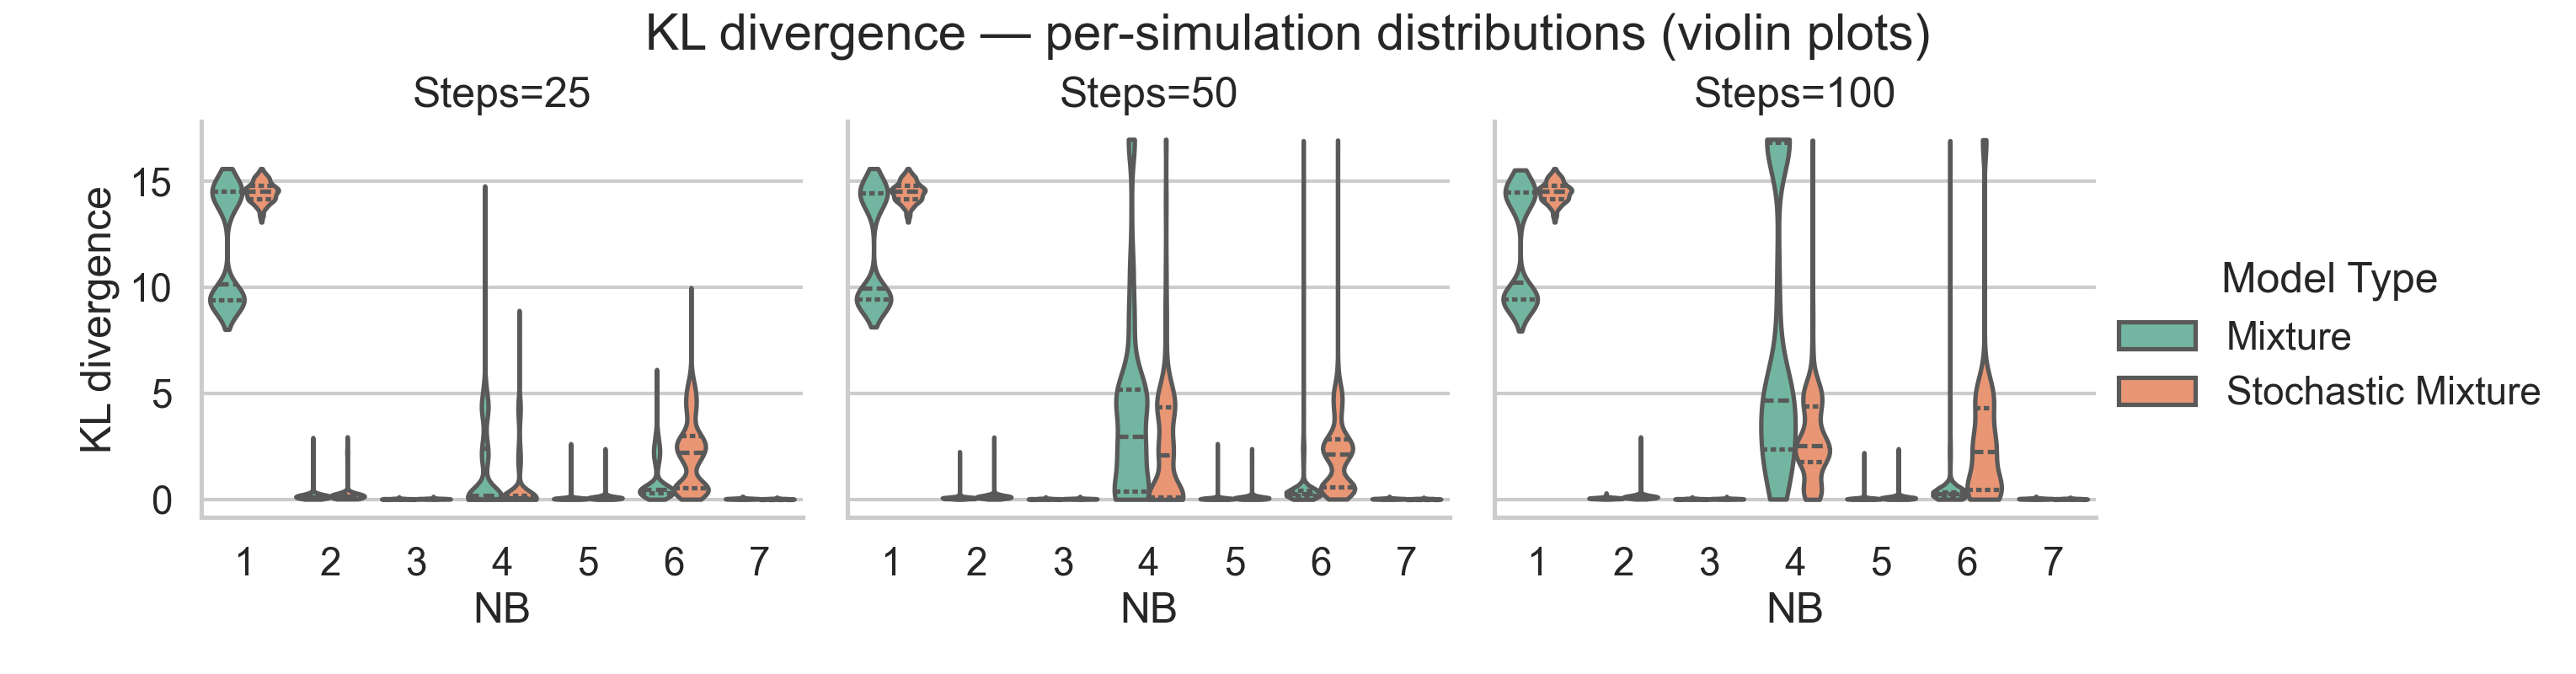
\includegraphics[width=\textwidth]{figs/neighborhood_analysis/nb_sweep_300x100/violin_KL_Divergence.png}
  \caption{Step 3: per-simulation violin plots for KL divergence. \textbf{Legend:} abscissa = neighbourhood size \(NB\); ordinate = KL divergence (lower is better); one violin per \((NB,\text{model})\); columns = step length (25, 50, 100); violin width = density of runs; inner line = quartiles.}
  \label{fig:impl:step3:violin:kl}
\end{figure}
\vspace{-0.5em}
\newpage

\begin{figure}[H]
  \centering
  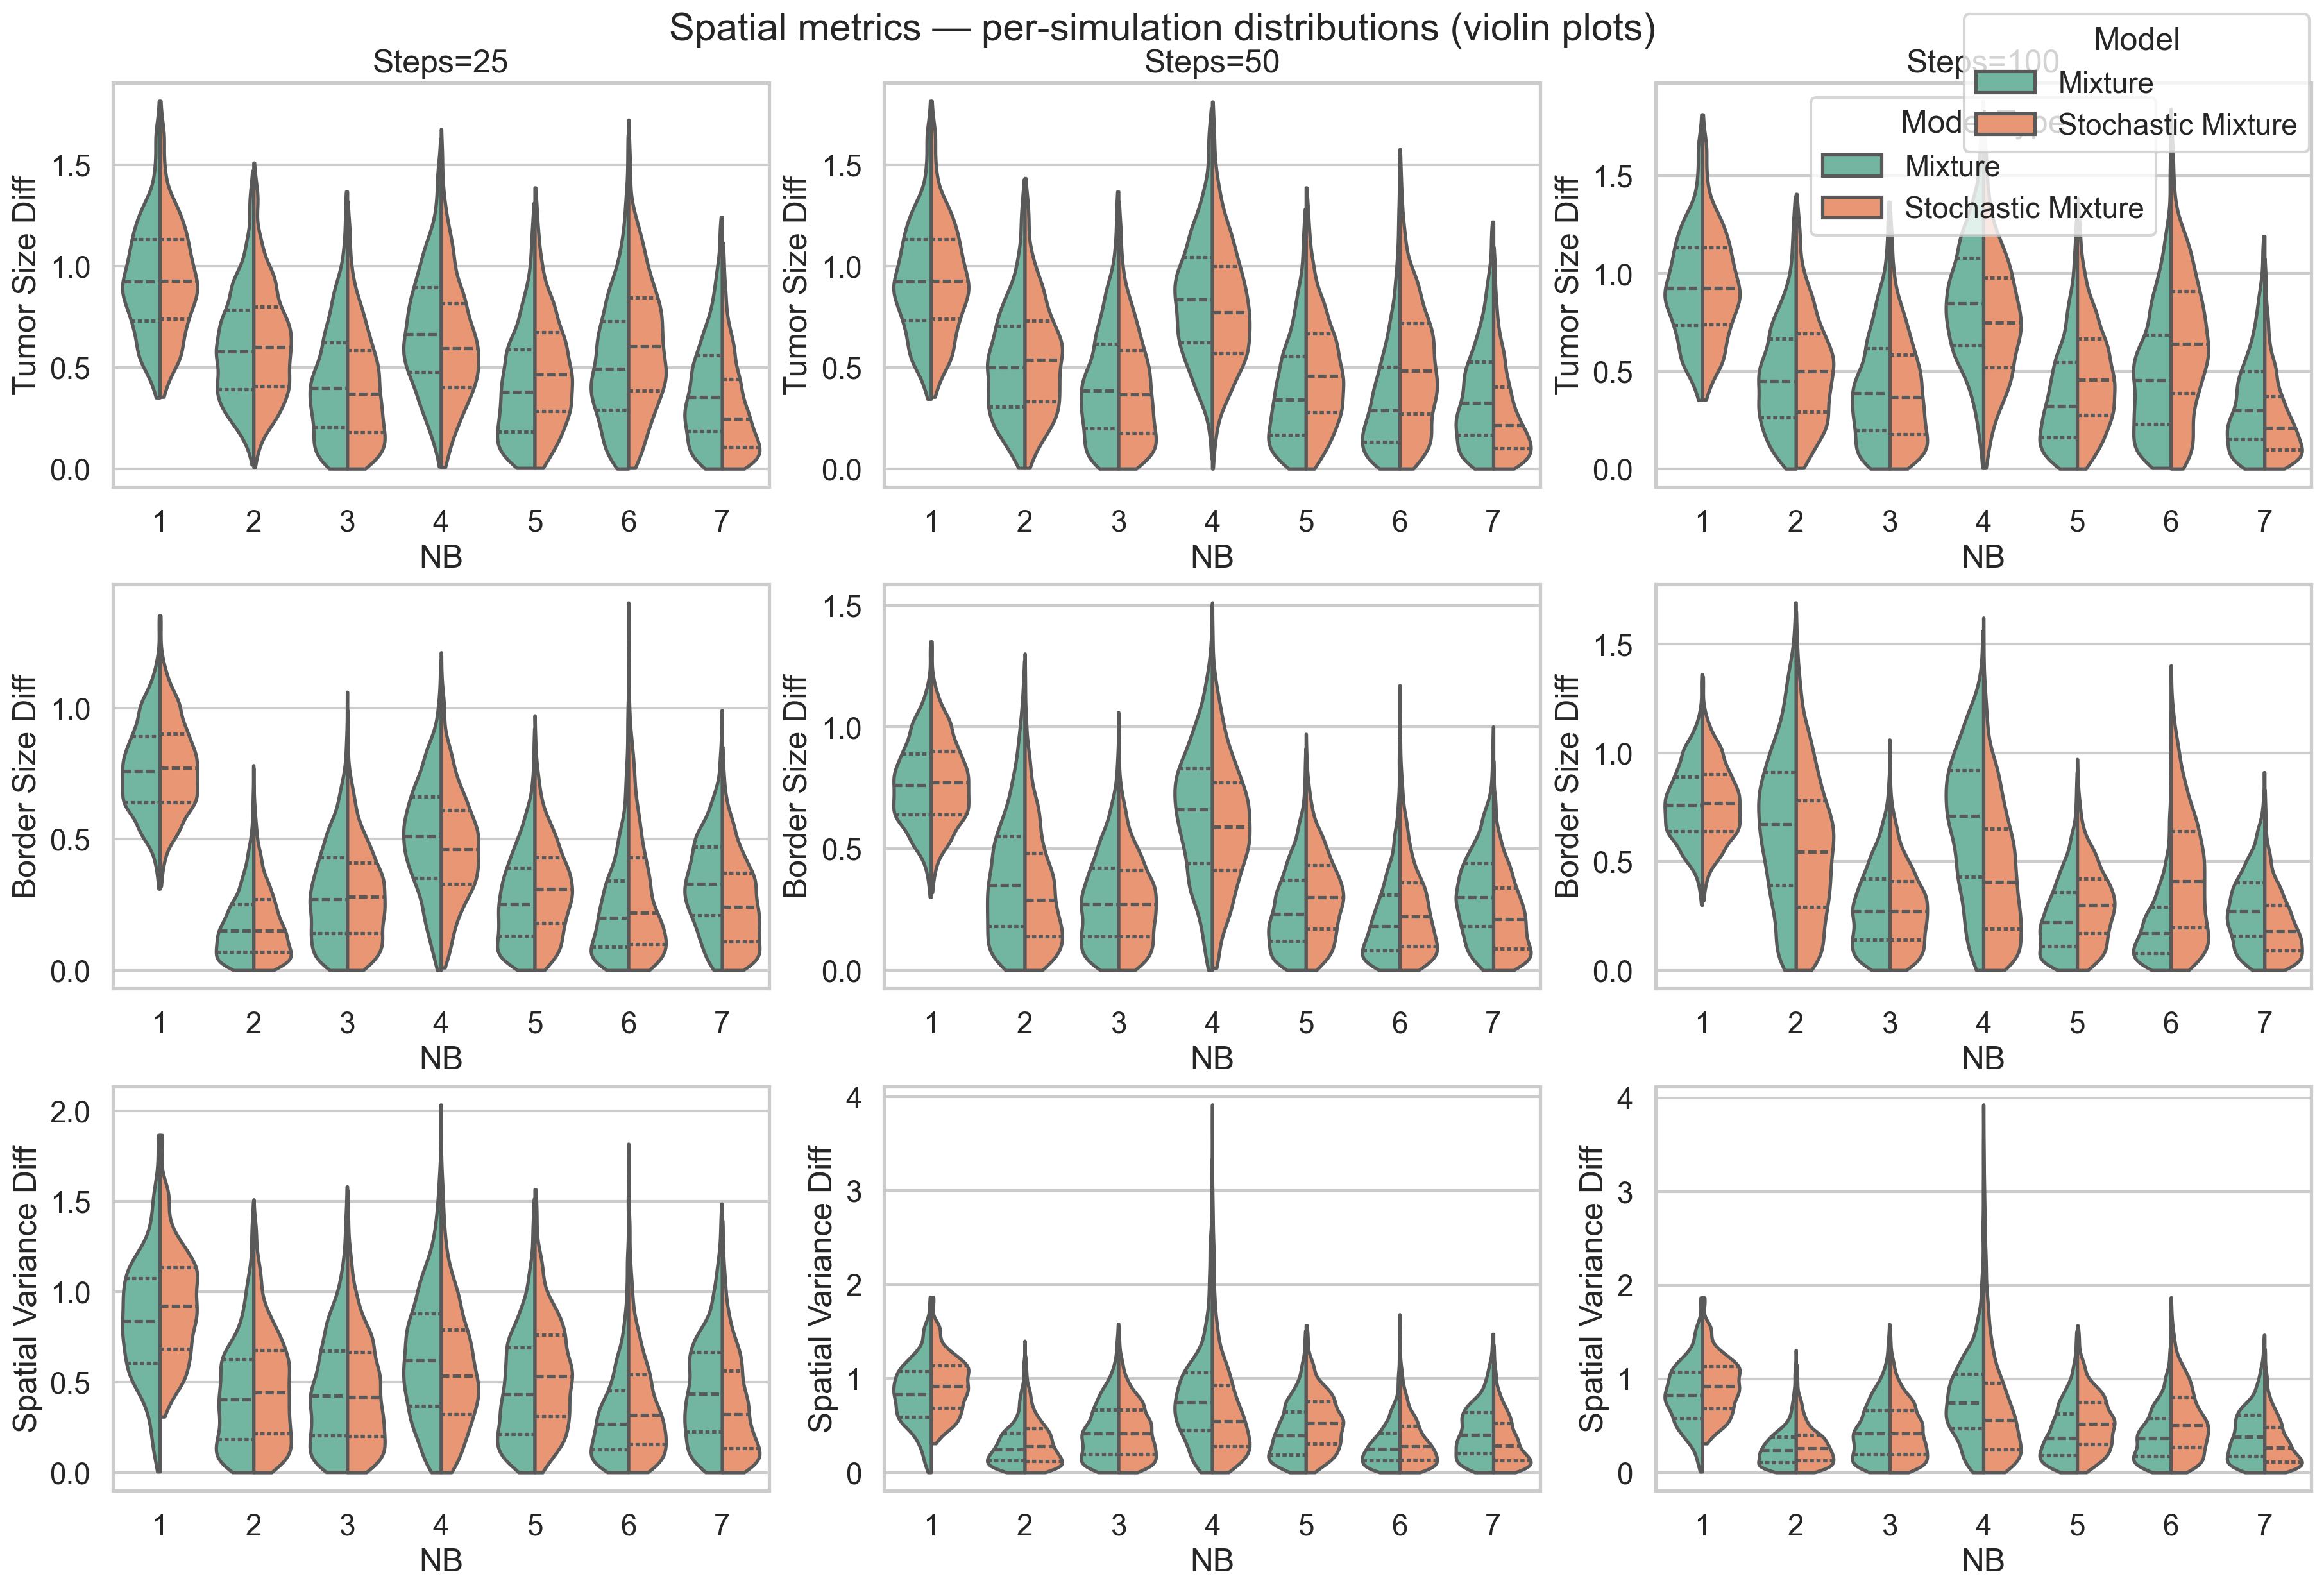
\includegraphics[width=\textwidth]{figs/neighborhood_analysis/nb_sweep_300x100/violin_spatial_metrics.png}
  \caption{Step 3: per-simulation violin plots for spatial metrics. \textbf{Legend:} three panels (tumour size difference, border size difference, spatial variance difference); abscissa = \(NB\); ordinate = metric value (lower is better); columns = step length; violin width = density, inner line = quartiles; series = Mixture vs.\ Stochastic Mixture NCA.}
  \label{fig:impl:step3:violin:spatial}
\end{figure}

\subsubsection{A dynamical bias--variance lens}
\label{sec:results:step3:biasvariance}
Although our setting is not classical supervised learning, the observed patterns can be interpreted through a \emph{structural and dynamical} bias--variance lens.
Here, \emph{bias} refers to systematic mismatch of the generated dynamics across simulations (persistently large mean errors), while \emph{variance} refers to sensitivity to stochastic fluctuations and failure modes (dispersion, heavy tails, and occasional large deviations in per-simulation distributions).
Under this view, \(NB=1\) corresponds to a high-bias regime: multiple metrics exhibit consistently large discrepancies, indicating that the receptive field is too limited to represent the relevant spatial couplings.
Moving to \(NB\in\{2,3\}\) reduces this structural bias sharply (Figure~\ref{fig:impl:step3:dashboard}) and often yields more concentrated per-simulation distributions (Figures~\ref{fig:impl:step3:violin:kl} and \ref{fig:impl:step3:violin:spatial}), although robustness remains metric-dependent (e.g.\ KL can still show substantial tail risk relative to the best configuration at a given horizon).
At intermediate neighbourhoods (notably around \(NB=4\), and for KL also \(NB=6\)), the mean performance can remain competitive while tail behaviour worsens (heavy tails and elevated bad-rate), i.e.\ a higher-variance regime in a dynamical sense.
For some metrics and horizons, larger neighbourhoods (especially \(NB=7\)) reduce tail risk again, consistent with stronger spatial averaging and more stable long-horizon rollouts; however, the overall picture remains non-monotonic and metric-specific, and in some spatial metrics \(NB=6\) can be preferable in mean even when KL robustness favors \(NB=7\).
Finally, these variance effects become more pronounced at longer rollout horizons, supporting the interpretation that neighbourhood size changes the \emph{dynamical regime} and that instability can be amplified over time rather than appearing immediately.

\subsubsection{Trend analysis and fold change}
\label{sec:results:step3:trend}

To summarise how performance changes with neighbourhood size in a compact way, we also compute a simple trend analysis over \(NB\).
In particular, we report fold change between a reference neighbourhood (here \(NB=3\), used as a normalization point in the sweep) and a larger neighbourhood (here \(NB=7\)).
On the plot, values below 1 indicate improvement when increasing neighbourhood size from 3 to 7, while values above 1 indicate degradation; the interpretation depends on the metric and on the rollout horizon.
This is useful because in several metrics the main effect is the jump from \(NB=1\) to \(NB\ge2\), while differences among \(NB\ge2\) are smaller and may depend on the metric.

\begin{figure}[H]
  \centering
  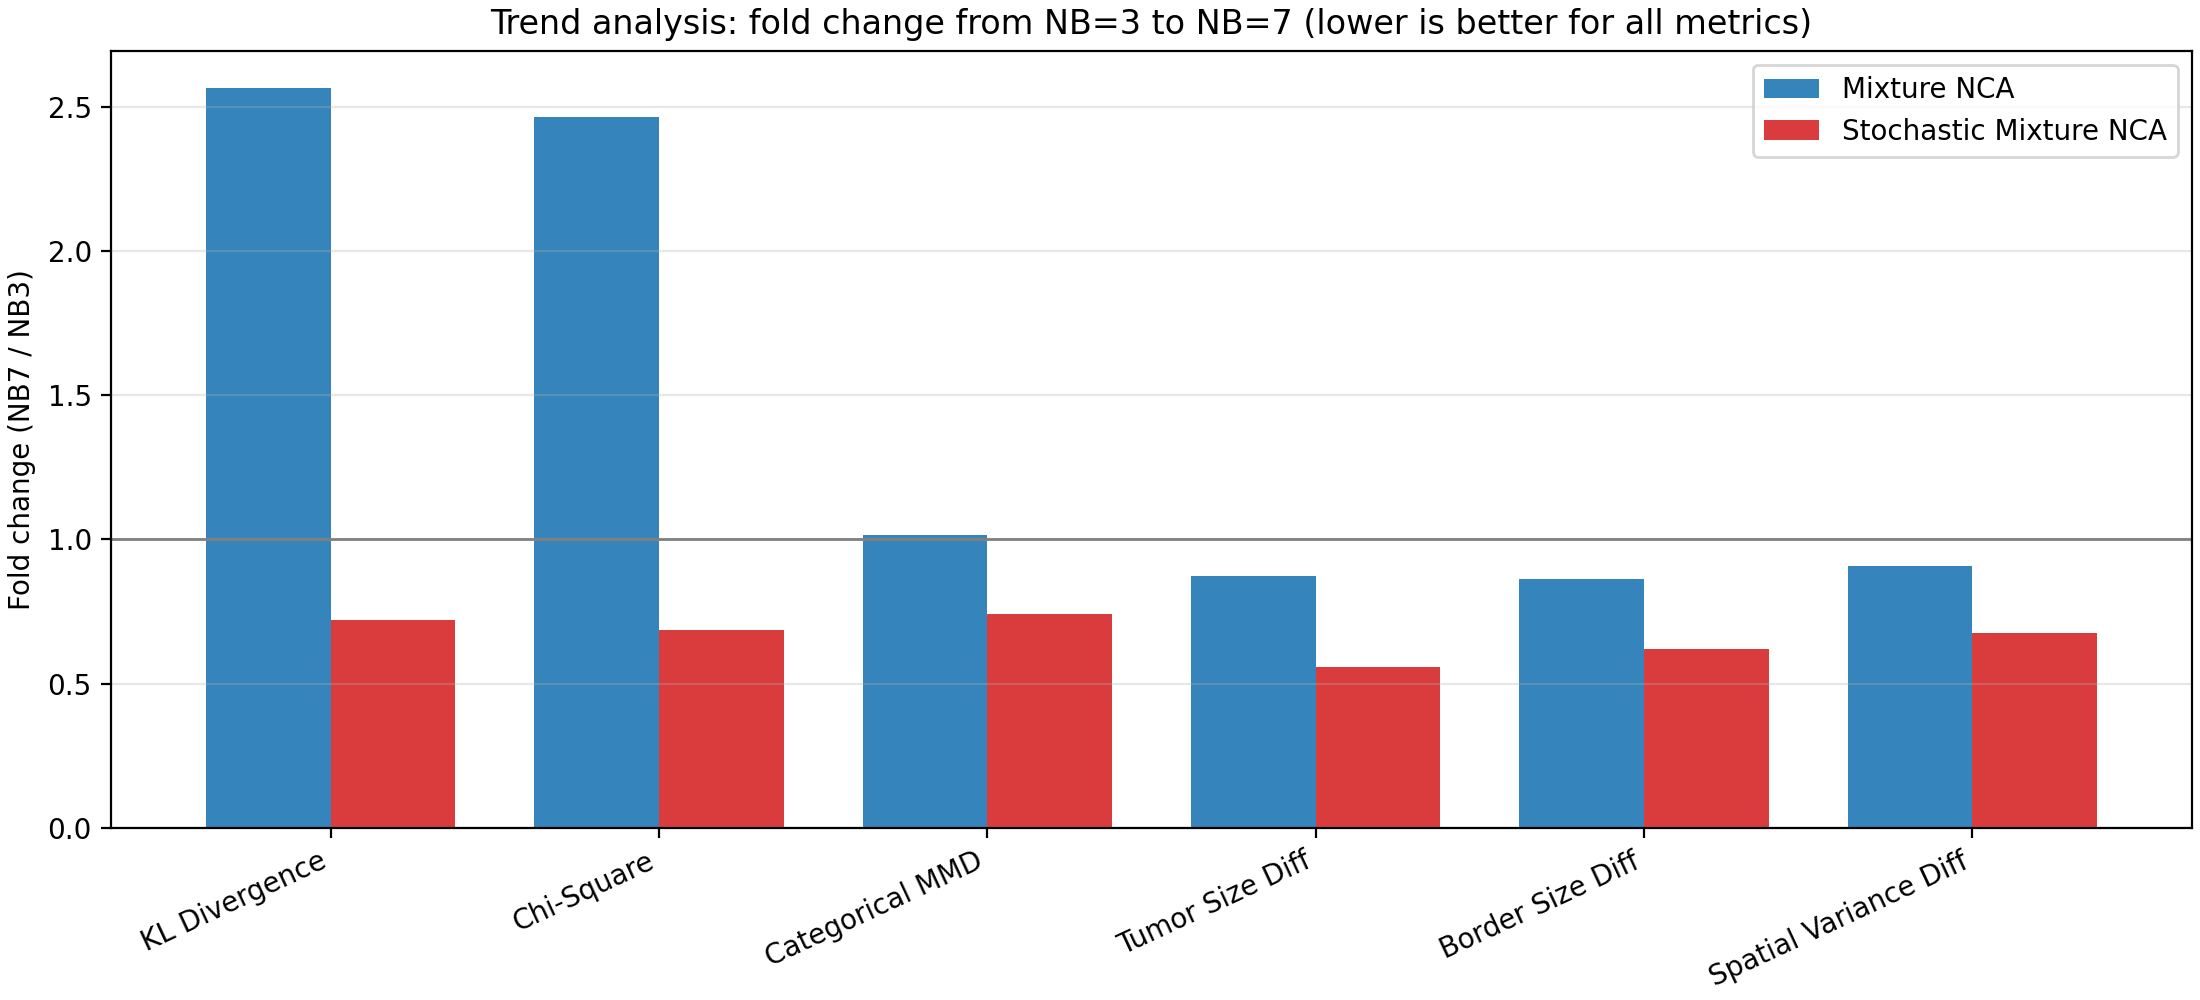
\includegraphics[width=\textwidth]{figs/neighborhood_analysis/nb_sweep_300x100/trend_foldchange_nb7_over_nb3.png}
  \caption{Step 3: trend analysis via fold change from \(NB=3\) to \(NB=7\). \textbf{Legend:} ratio \(\mathrm{metric}(NB=7)/\mathrm{metric}(NB=3)\) on the ordinate (reference line at 1); abscissa = metric; panels by step length and model type.}
  \label{fig:impl:step3:trend:foldchange}
\end{figure}

\subsubsection{Robustness via bad-rate}
\label{sec:results:step3:badrate}

Mean values alone can hide important instability: per-simulation distributions often show heavy tails where a non-trivial fraction of runs ends in poor outcomes (``failure modes'').
To quantify this, we define a \emph{bad-rate} as follows: for each metric and each (model, step length), we select the neighbourhood size with the best median performance, take the 95th percentile of that best distribution as a threshold, and compute for each \(NB\) the probability that a run exceeds this threshold.

\begin{figure}[H]
  \centering
  
\includegraphics[width=\textwidth]{figs/neighborhood_analysis/nb_sweep_300x100/badrate_bars_KL_Divergence.png}
  \caption{Step 3: bad-rate for KL divergence. \textbf{Legend:} abscissa = \(NB\); ordinate = fraction of runs whose KL exceeds the 95th percentile of the best \(NB\) for that (model, step length); columns = step length; bars = Mixture vs.\ Stochastic Mixture NCA; lower is better.}
  \label{fig:impl:step3:badrate:kl}
\end{figure}

\begin{figure}[H]
  \centering
  
\includegraphics[width=\textwidth]{figs/neighborhood_analysis/nb_sweep_300x100/badrate_bars_Tumor_Size_Diff.png}
  \caption{Step 3: bad-rate for tumour size difference. \textbf{Legend:} same as Figure~\ref{fig:impl:step3:badrate:kl} (abscissa = \(NB\), ordinate = fraction of runs above threshold, columns = step length, series = model type; lower is better).}
  \label{fig:impl:step3:badrate:tumor}
\end{figure}

\begin{figure}[H]
  \centering
  
\includegraphics[width=\textwidth]{figs/neighborhood_analysis/nb_sweep_300x100/badrate_bars_Border_Size_Diff.png}
  \caption{Step 3: bad-rate for border size difference. \textbf{Legend:} same layout as Figure~\ref{fig:impl:step3:badrate:kl} (abscissa = \(NB\), ordinate = bad-rate fraction, columns = step length; lower is better).}
  \label{fig:impl:step3:badrate:border}
\end{figure}

\begin{figure}[H]
  \centering
  
\includegraphics[width=\textwidth]{figs/neighborhood_analysis/nb_sweep_300x100/badrate_bars_Spatial_Variance_Diff.png}
  \caption{Step 3: bad-rate for spatial variance difference. \textbf{Legend:} same layout as Figure~\ref{fig:impl:step3:badrate:kl} (abscissa = \(NB\), ordinate = bad-rate fraction, columns = step length; lower is better).}
  \label{fig:impl:step3:badrate:spvar}
\end{figure}

\subsubsection{Computational complexity and rule specialization}
\label{sec:results:step3:complexity_rules}

Figure~\ref{fig:impl:step3:complexity} reports the empirical runtime as a function of neighbourhood size.
In the explored range \(NB\in[1,7]\), the measured runtime remains approximately flat.
Empirically, Mixture NCA runs at about \(\sim 1.5\) ms/step on average, while the Stochastic Mixture variant is about \(\sim 3.2\) ms/step, with limited variation across neighbourhood size.
This suggests that in this implementation range the practical cost is dominated by constants and vectorization effects rather than by the naive theoretical \(O(NB^2)\) scaling.

\begin{figure}[H]
  \centering
  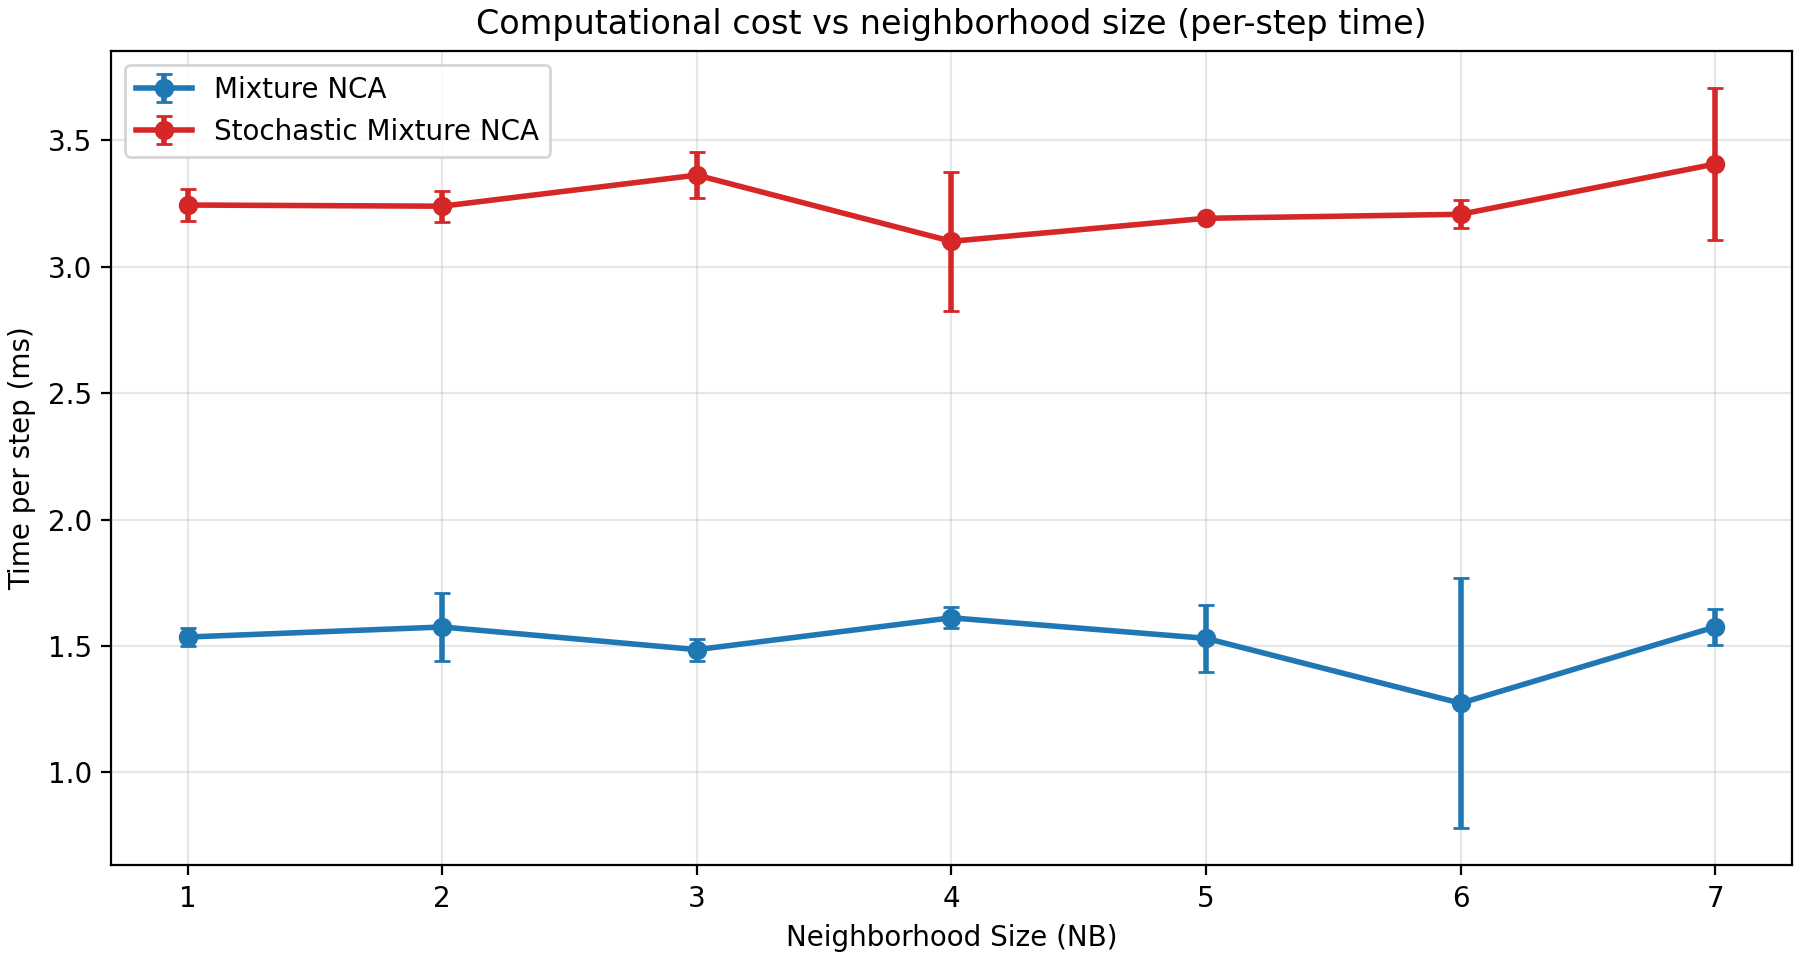
\includegraphics[width=0.85\textwidth]{figs/neighborhood_analysis/nb_sweep_300x100/computational_complexity_time_per_step.png}
  \caption{Step 3: empirical computational cost vs neighbourhood size. \textbf{Legend:} abscissa = \(NB\); ordinate = time per simulation step (ms); two series = Mixture NCA and Stochastic Mixture NCA; error bars = variability over repeated timing runs.}
  \label{fig:impl:step3:complexity}
\end{figure}

\begin{figure}[H]
  \centering
  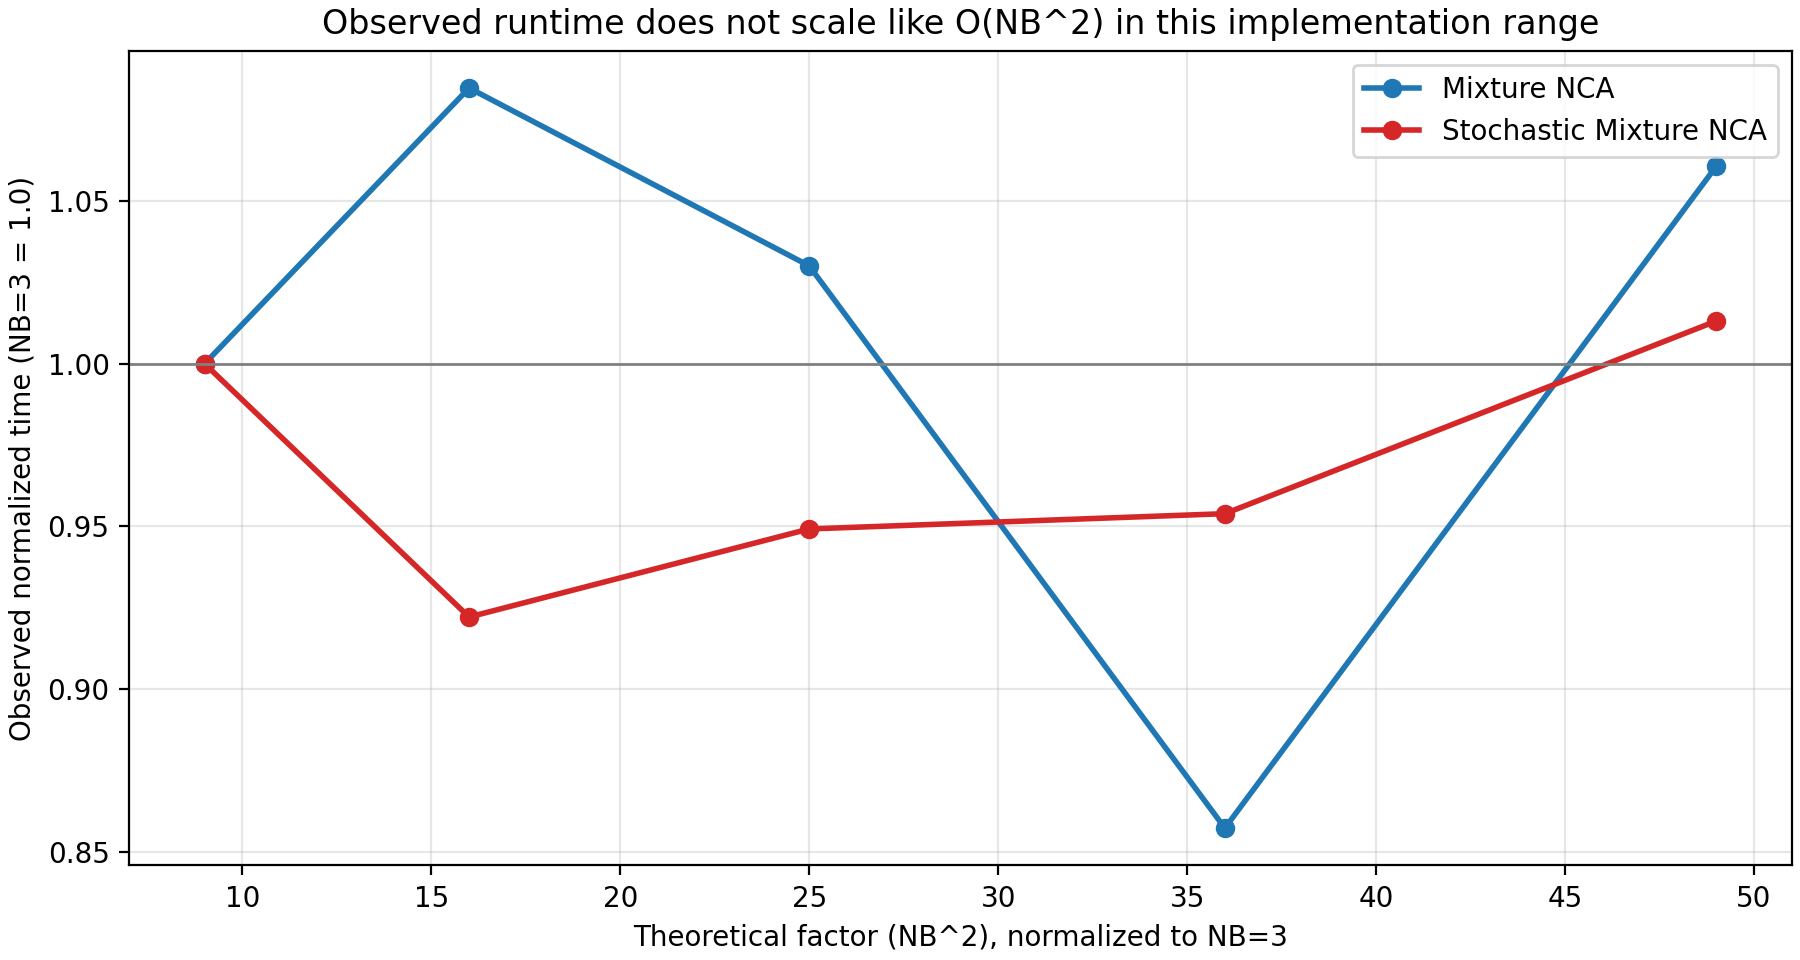
\includegraphics[width=0.85\textwidth]{figs/neighborhood_analysis/nb_sweep_300x100/computational_complexity_normalized_vs_theory.png}
  \caption{Step 3: normalized runtime vs.\ \(NB\). \textbf{Legend:} abscissa = \(NB\); ordinate = time relative to \(NB=3\) (value 1.0 = same as \(NB=3\)); series = Mixture vs.\ Stochastic Mixture NCA.}
  \label{fig:impl:step3:complexity:theory}
\end{figure}

Finally, we analyze how rules are selected over time as a function of neighbourhood size, which provides a qualitative explanation for the observed trade-offs and stability differences.
To study how specialization evolves during the dynamics, we measure the entropy of the model's rule-assignment distribution \(p(r \mid x_t)\) at each time step, averaged over space and over sampled simulations.
Low entropy indicates confident (specialized) rule selection, while higher entropy indicates mixed or uncertain rule usage.

\begin{figure}[H]
  \centering
  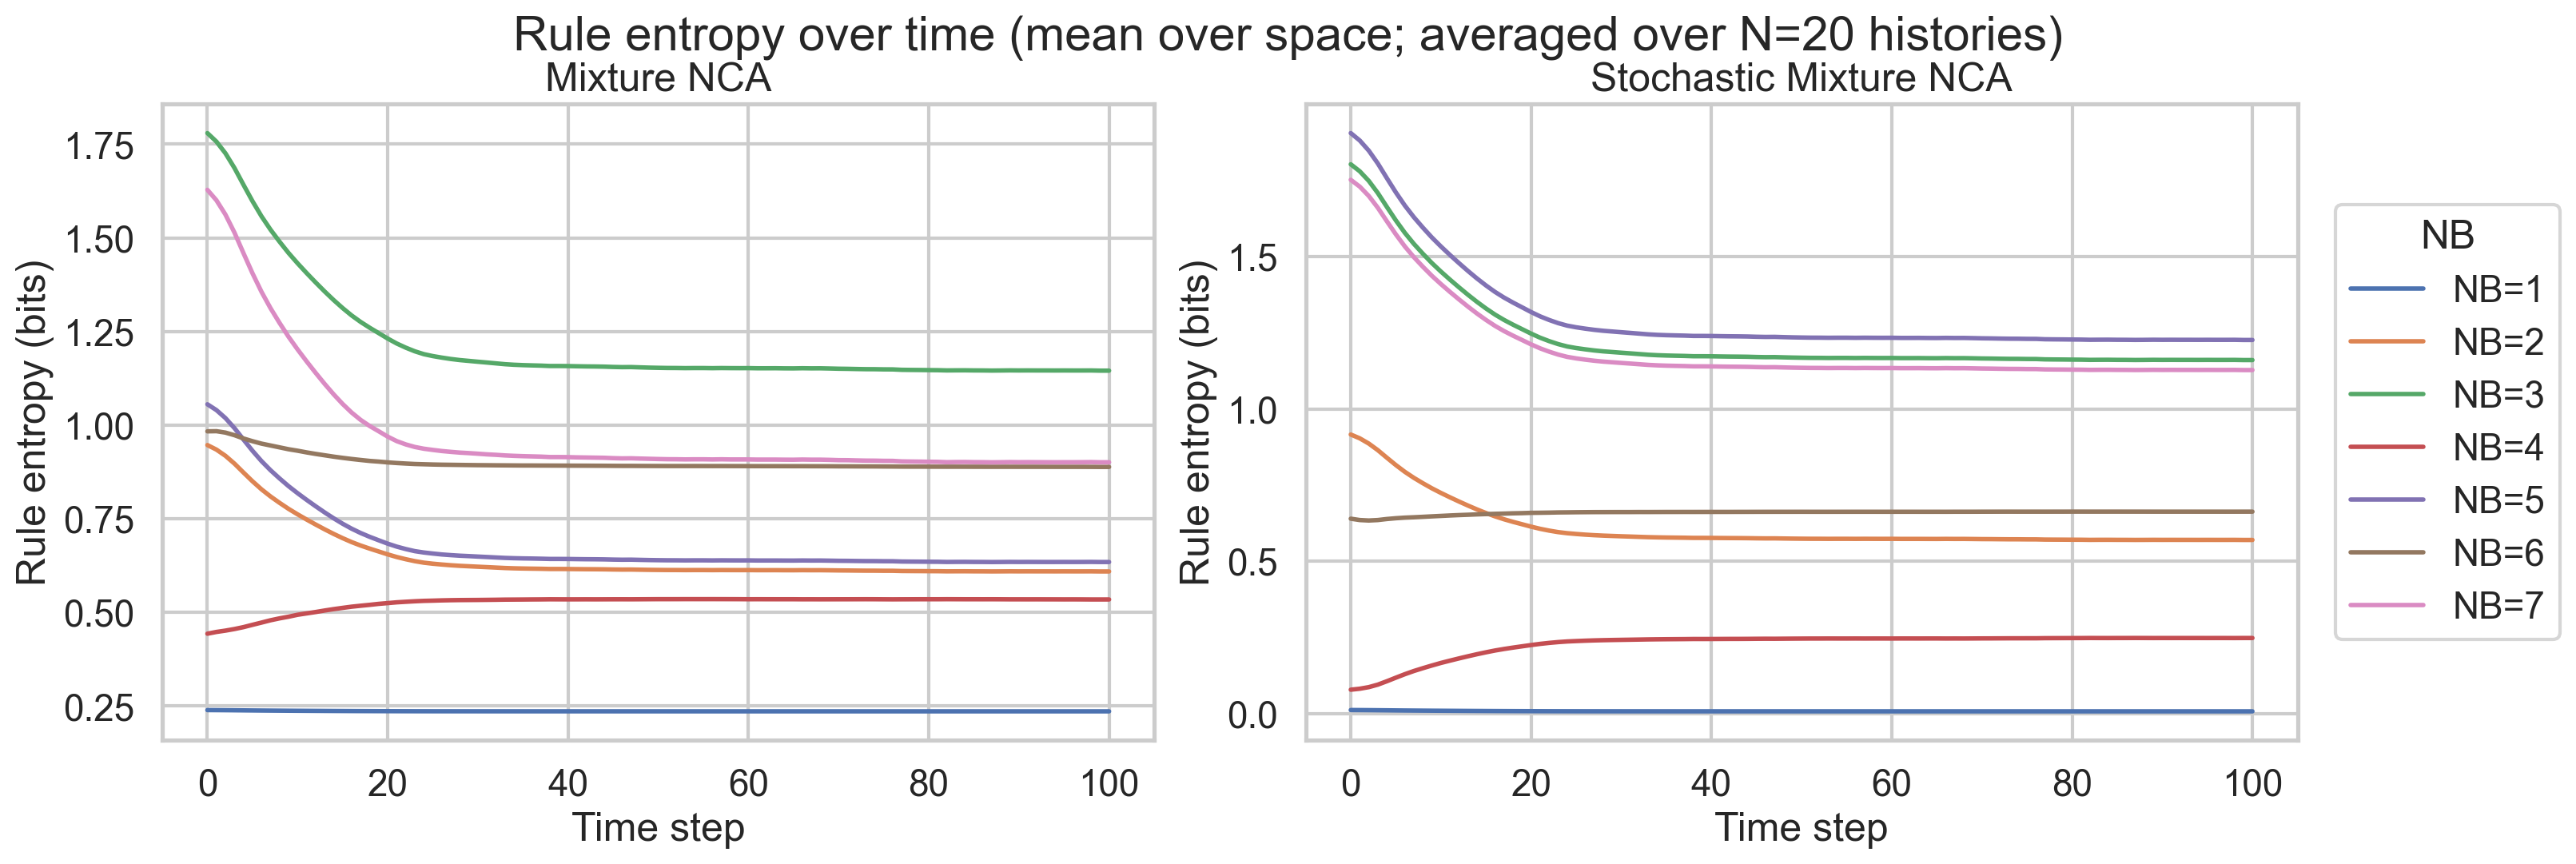
\includegraphics[width=\textwidth]{figs/neighborhood_analysis/nb_sweep_300x100/rule_entropy_over_time.png}
  \caption{Step 3: rule-assignment entropy over time. \textbf{Legend:} abscissa = simulation step; ordinate = entropy (bits), averaged over space and over \(N=20\) histories; one curve per neighbourhood size \(NB\); left panel = Mixture NCA, right panel = Stochastic Mixture NCA.}
  \label{fig:impl:step3:entropy:time}
\end{figure}

To complement the time-series view, we also summarize rule specialization with three simple indicators:
\begin{itemize}
  \item mean entropy (lower means more confident selection),
  \item rule diversity (higher means probability mass is spread over more rules),
  \item max rule usage (the maximum average probability assigned to a single rule; lower means more balanced usage).
\end{itemize}
Figure~\ref{fig:impl:step3:rule:summary} reports these indicators and relates them to KL divergence at Step Length \(=100\).
The resulting scatter does \emph{not} support a simple inverse (or linear) relation between specialization and dynamic divergence once \(NB\ge2\).
KL divergence is large mainly in the strongly constrained regime (\(NB=1\)): the model can commit confidently (low entropy) while still producing a large distributional mismatch, because it lacks spatial context and the resulting dynamics drift toward wrong global compositions.
For \(NB\ge2\), configurations with higher entropy (more mixed rule usage) can achieve equally low or even lower KL than more specialized ones, suggesting that mescolanza can be compatible with (and in some cases associated with) more stable long-horizon dynamics.
Therefore, rule specialization should be treated as a diagnostic of the operating regime (constraint vs.\ flexibility) rather than as a direct predictor of distributional fidelity.

\begin{figure}[H]
  \centering
  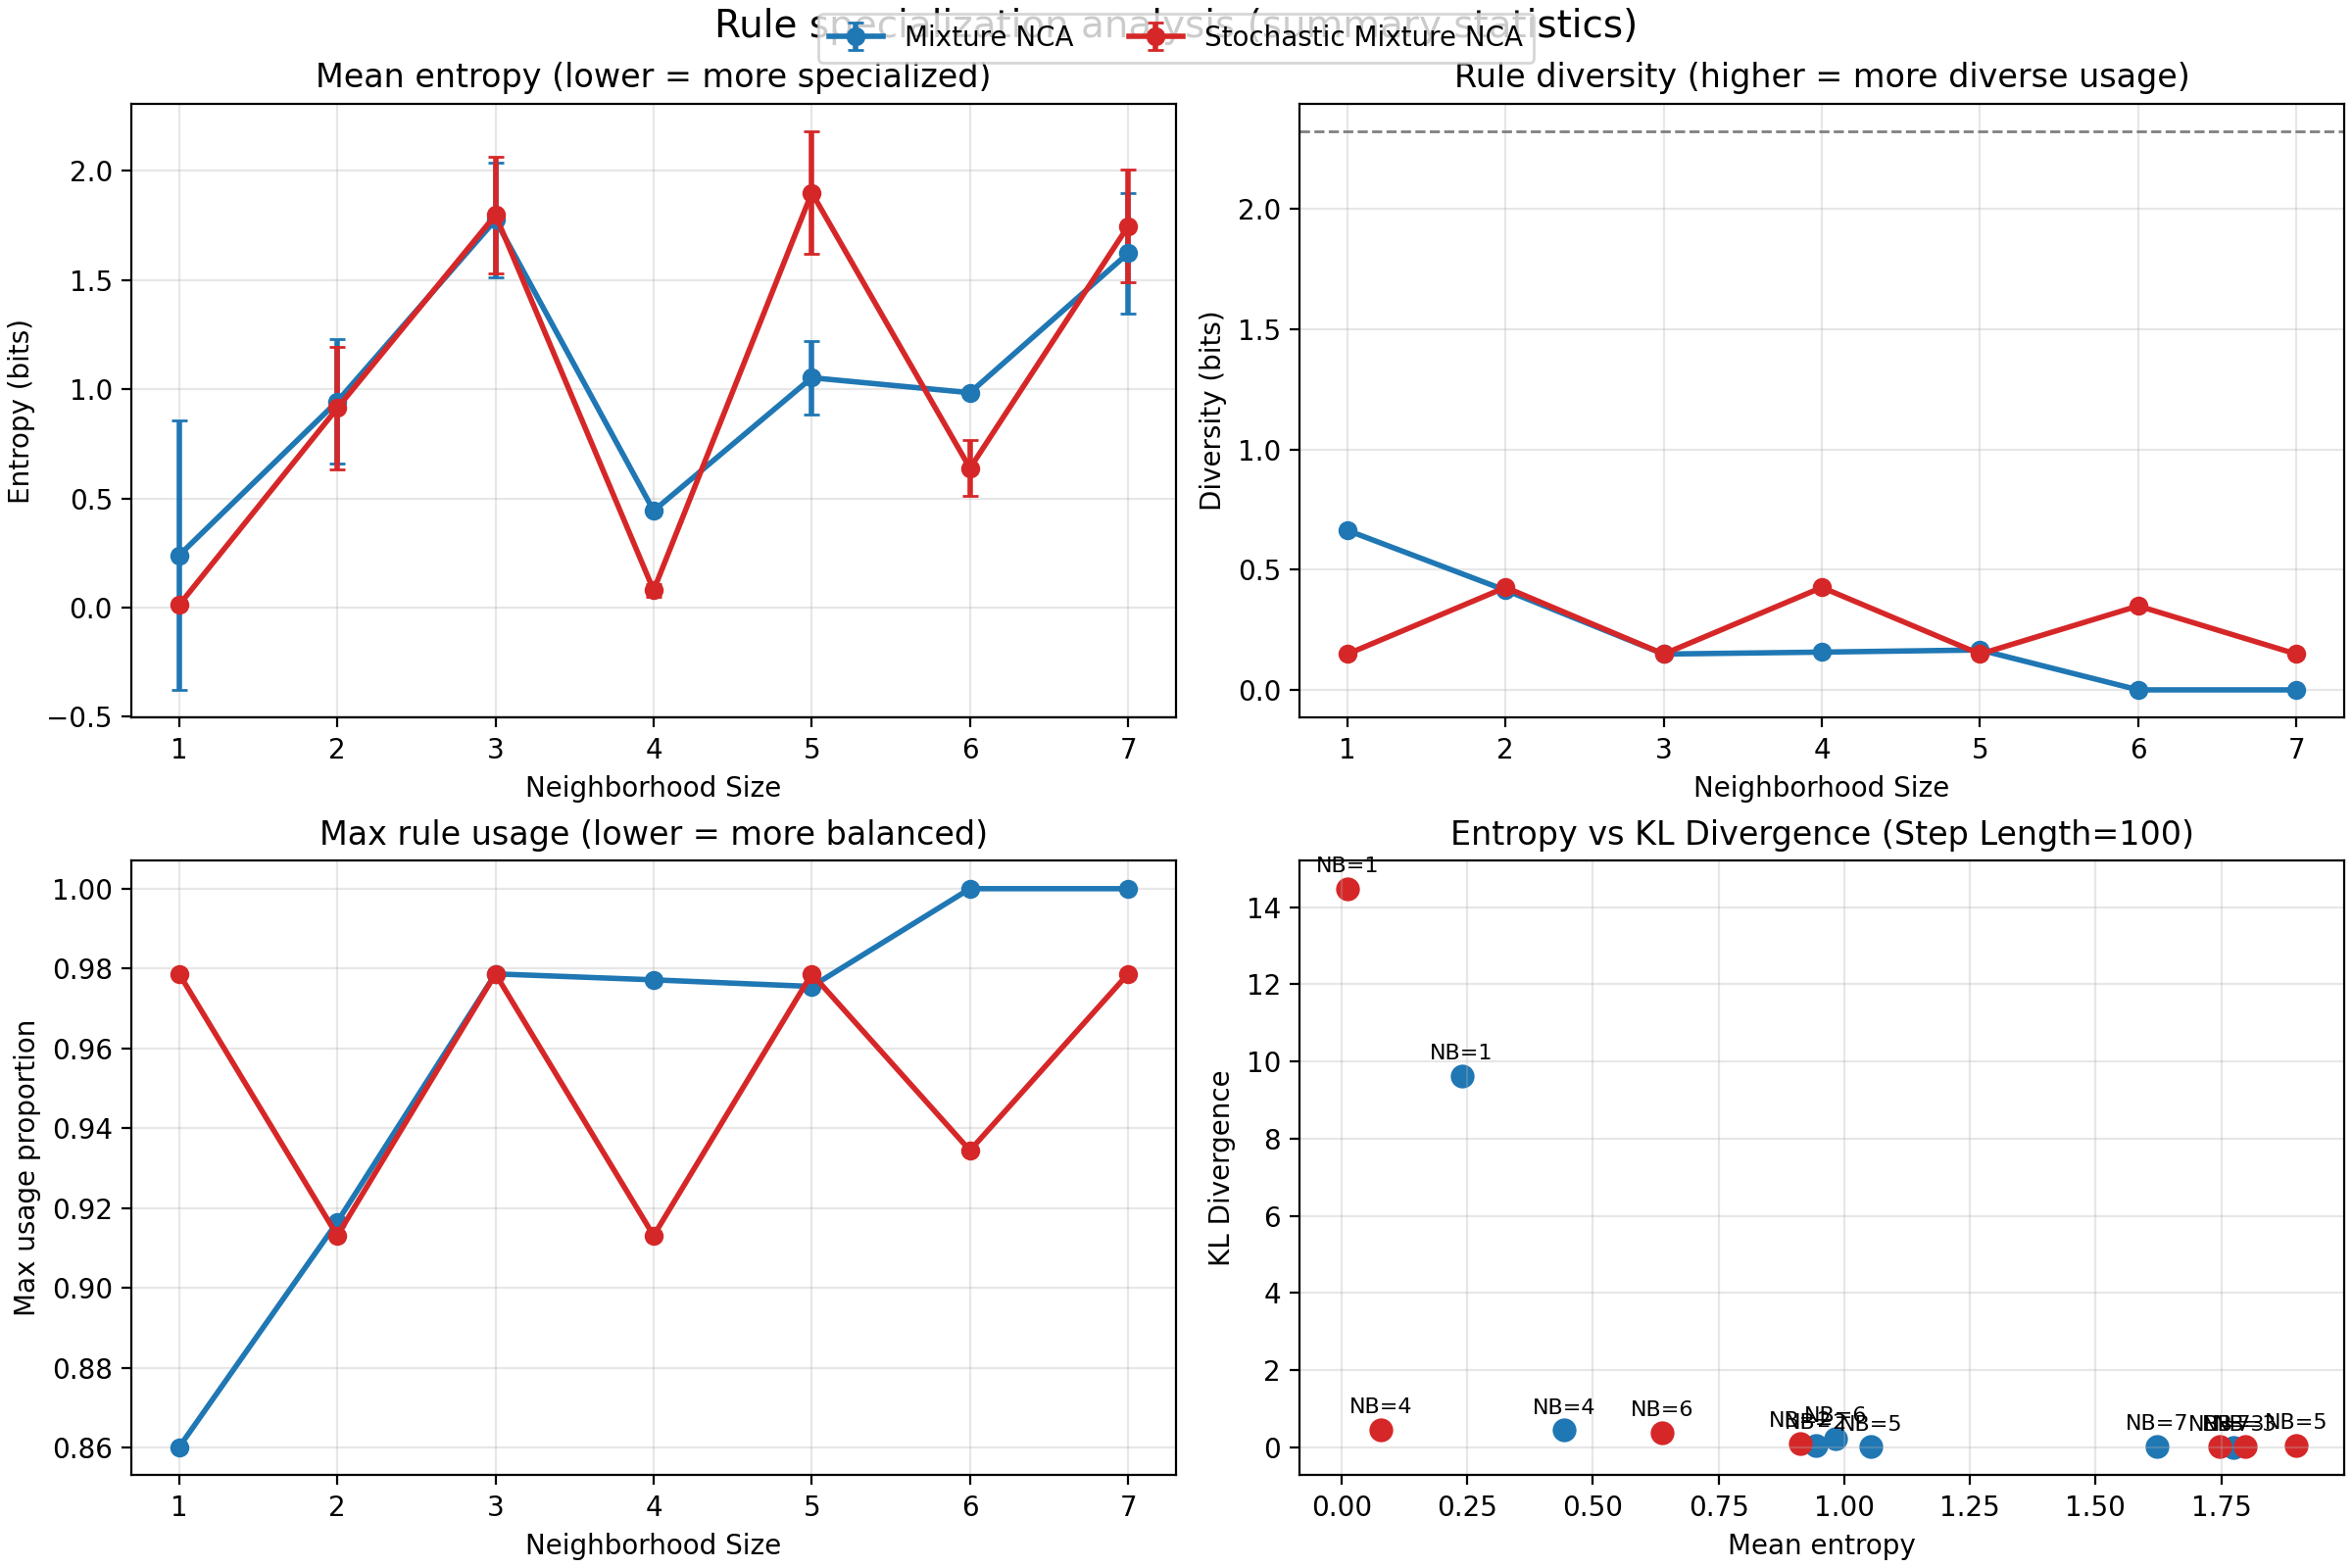
\includegraphics[width=\textwidth]{figs/neighborhood_analysis/nb_sweep_300x100/rule_specialization_summary.png}
  \caption{Step 3: rule specialization summary. \textbf{Legend:} four panels (mean entropy, rule diversity, max rule share, and scatter entropy vs.\ KL at step length 100); points/series = neighbourhood sizes \(NB\); bottom-right panel: abscissa = entropy, ordinate = KL divergence at step length 100.}
  \label{fig:impl:step3:rule:summary}
\end{figure}

\newpage
To make rule selection more intuitive, we also visualize the \emph{rule-assignment probability maps} \(p(r \mid x)\) for a single example state.
Each heatmap shows, for each spatial position, how likely the model is to select a given rule, and the rows compare selected neighbourhood sizes.

\begin{figure}[H]
  \centering
  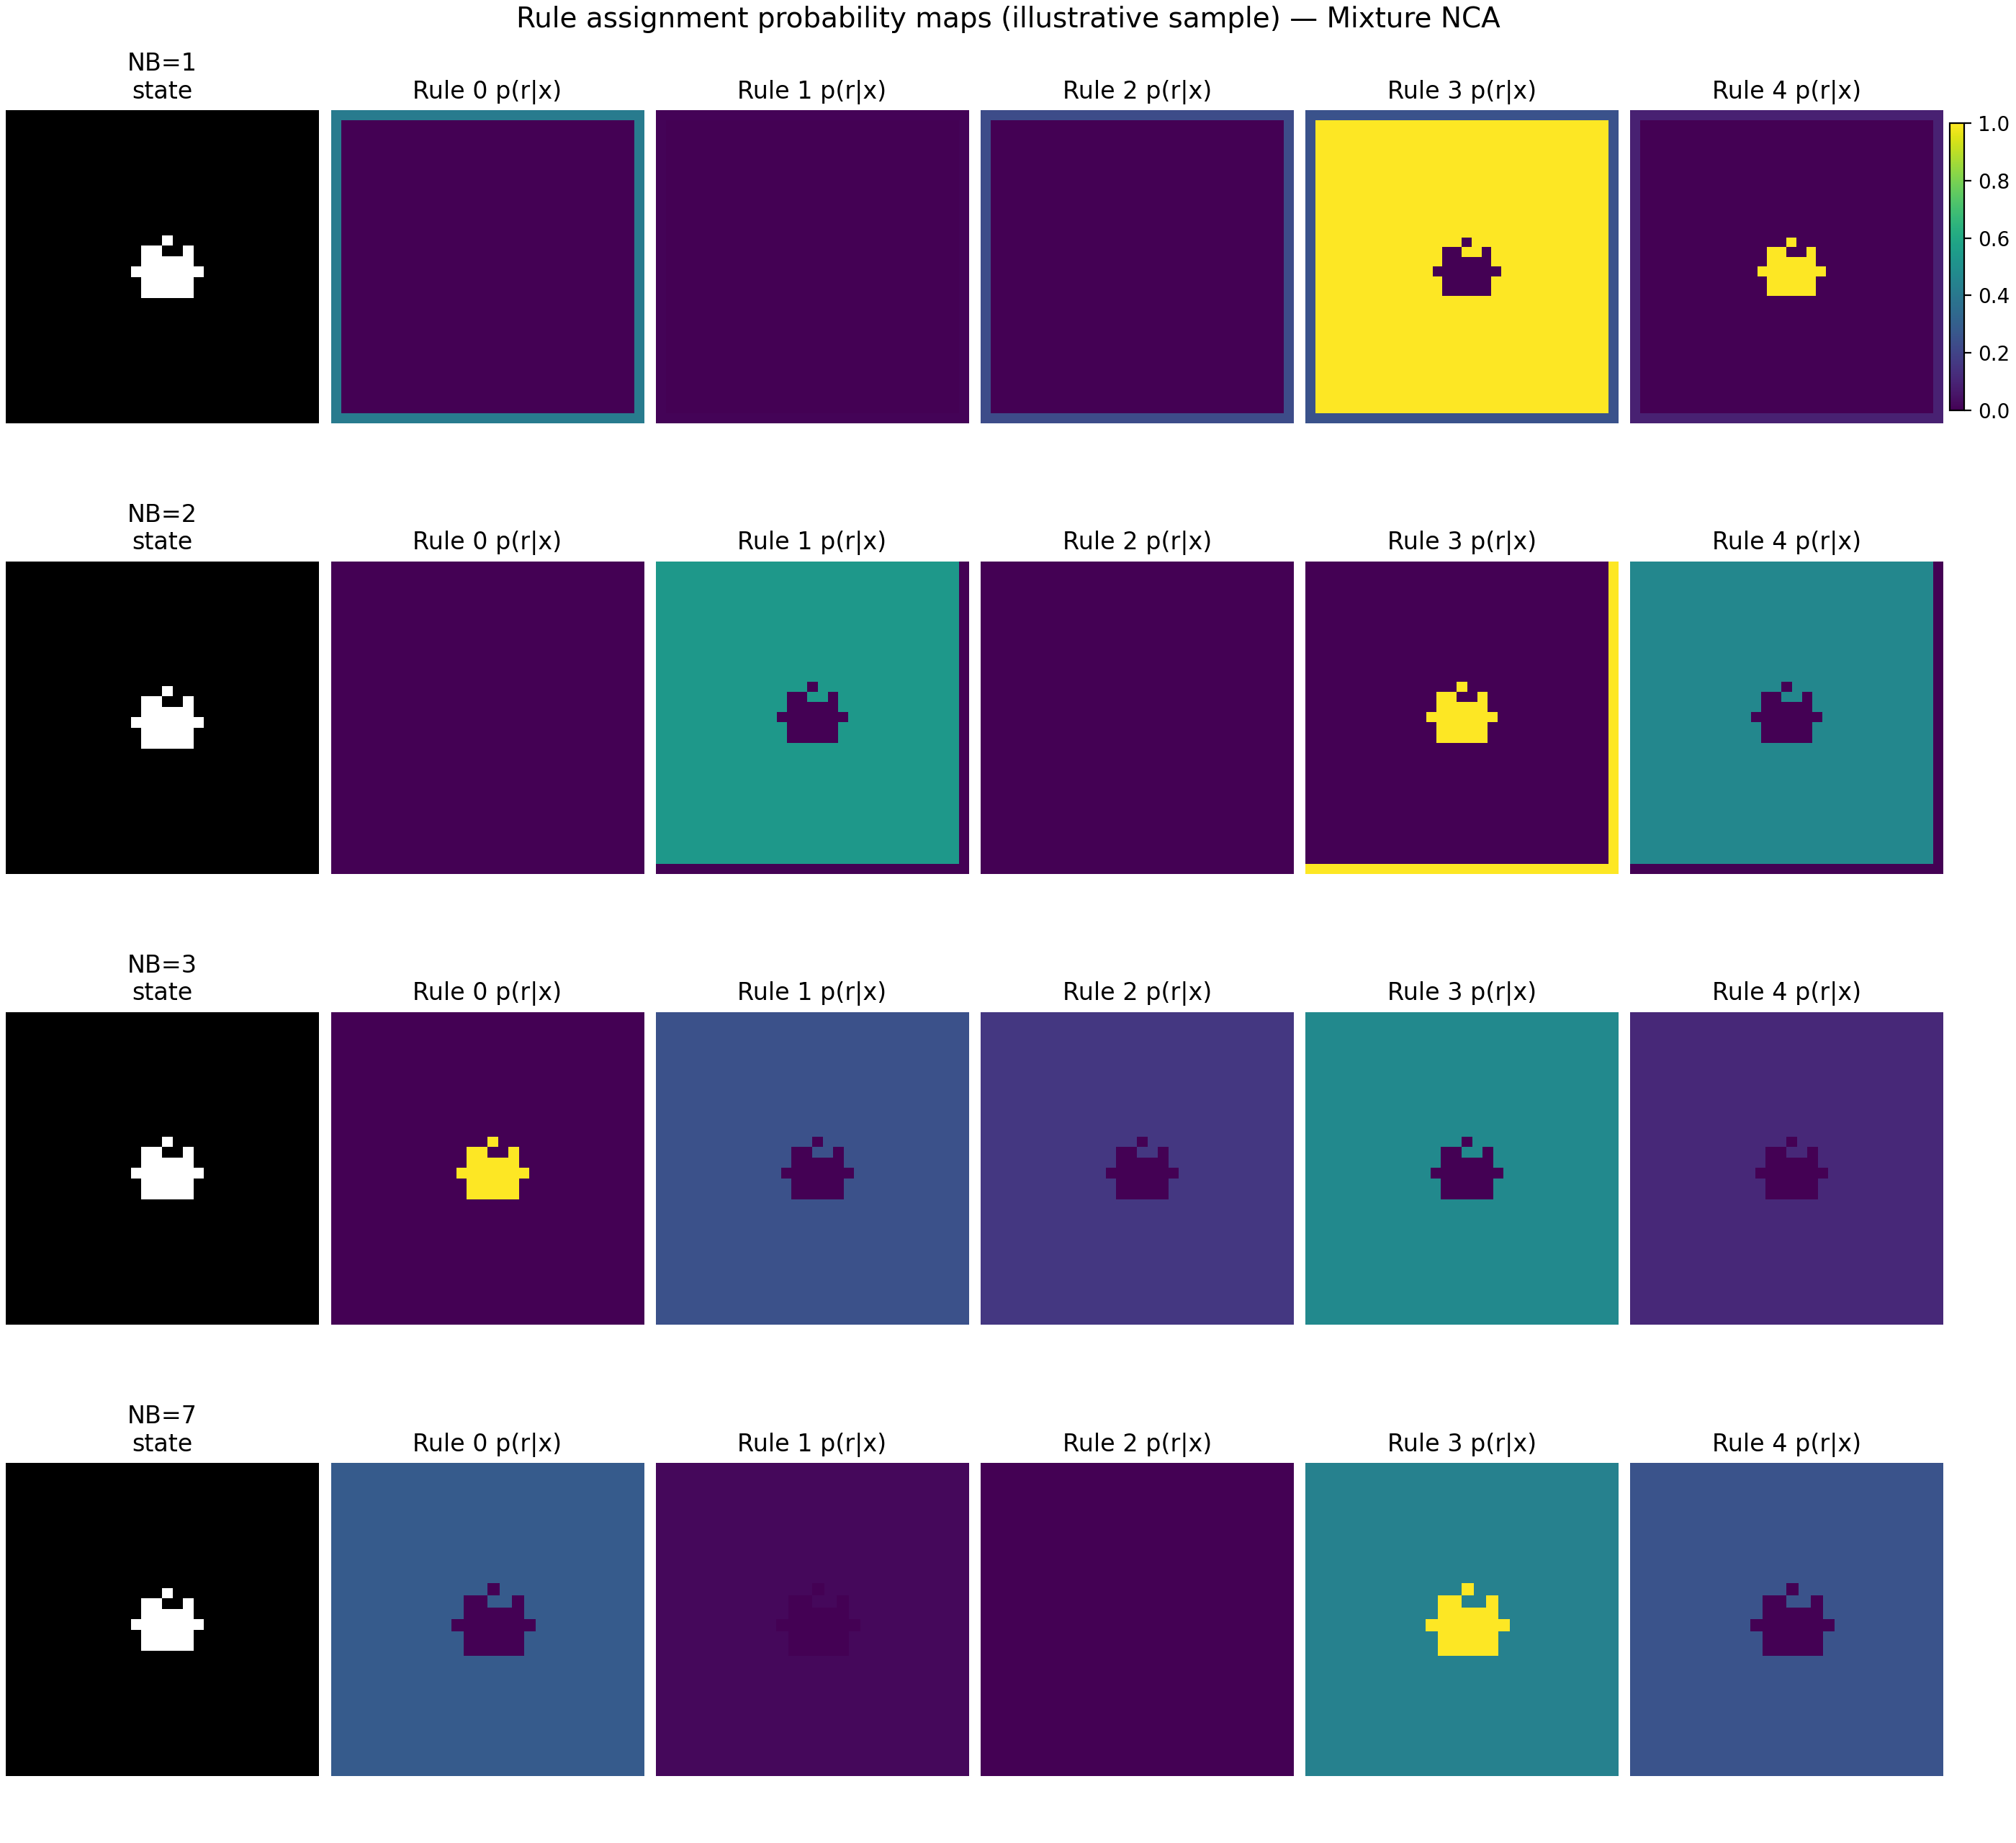
\includegraphics[width=\textwidth]{figs/neighborhood_analysis/nb_sweep_300x100/rule_assignment_maps_mixture.png}
  \caption{Step 3: rule assignment probability maps for Mixture NCA (one example state). \textbf{Legend:} columns = input state and probability map for each of the five rules; rows = neighbourhood size \(NB\); colour intensity = probability of selecting that rule at each cell.}
  \label{fig:impl:step3:rule:maps:mix}
\end{figure}

\begin{figure}[H]
  \centering
  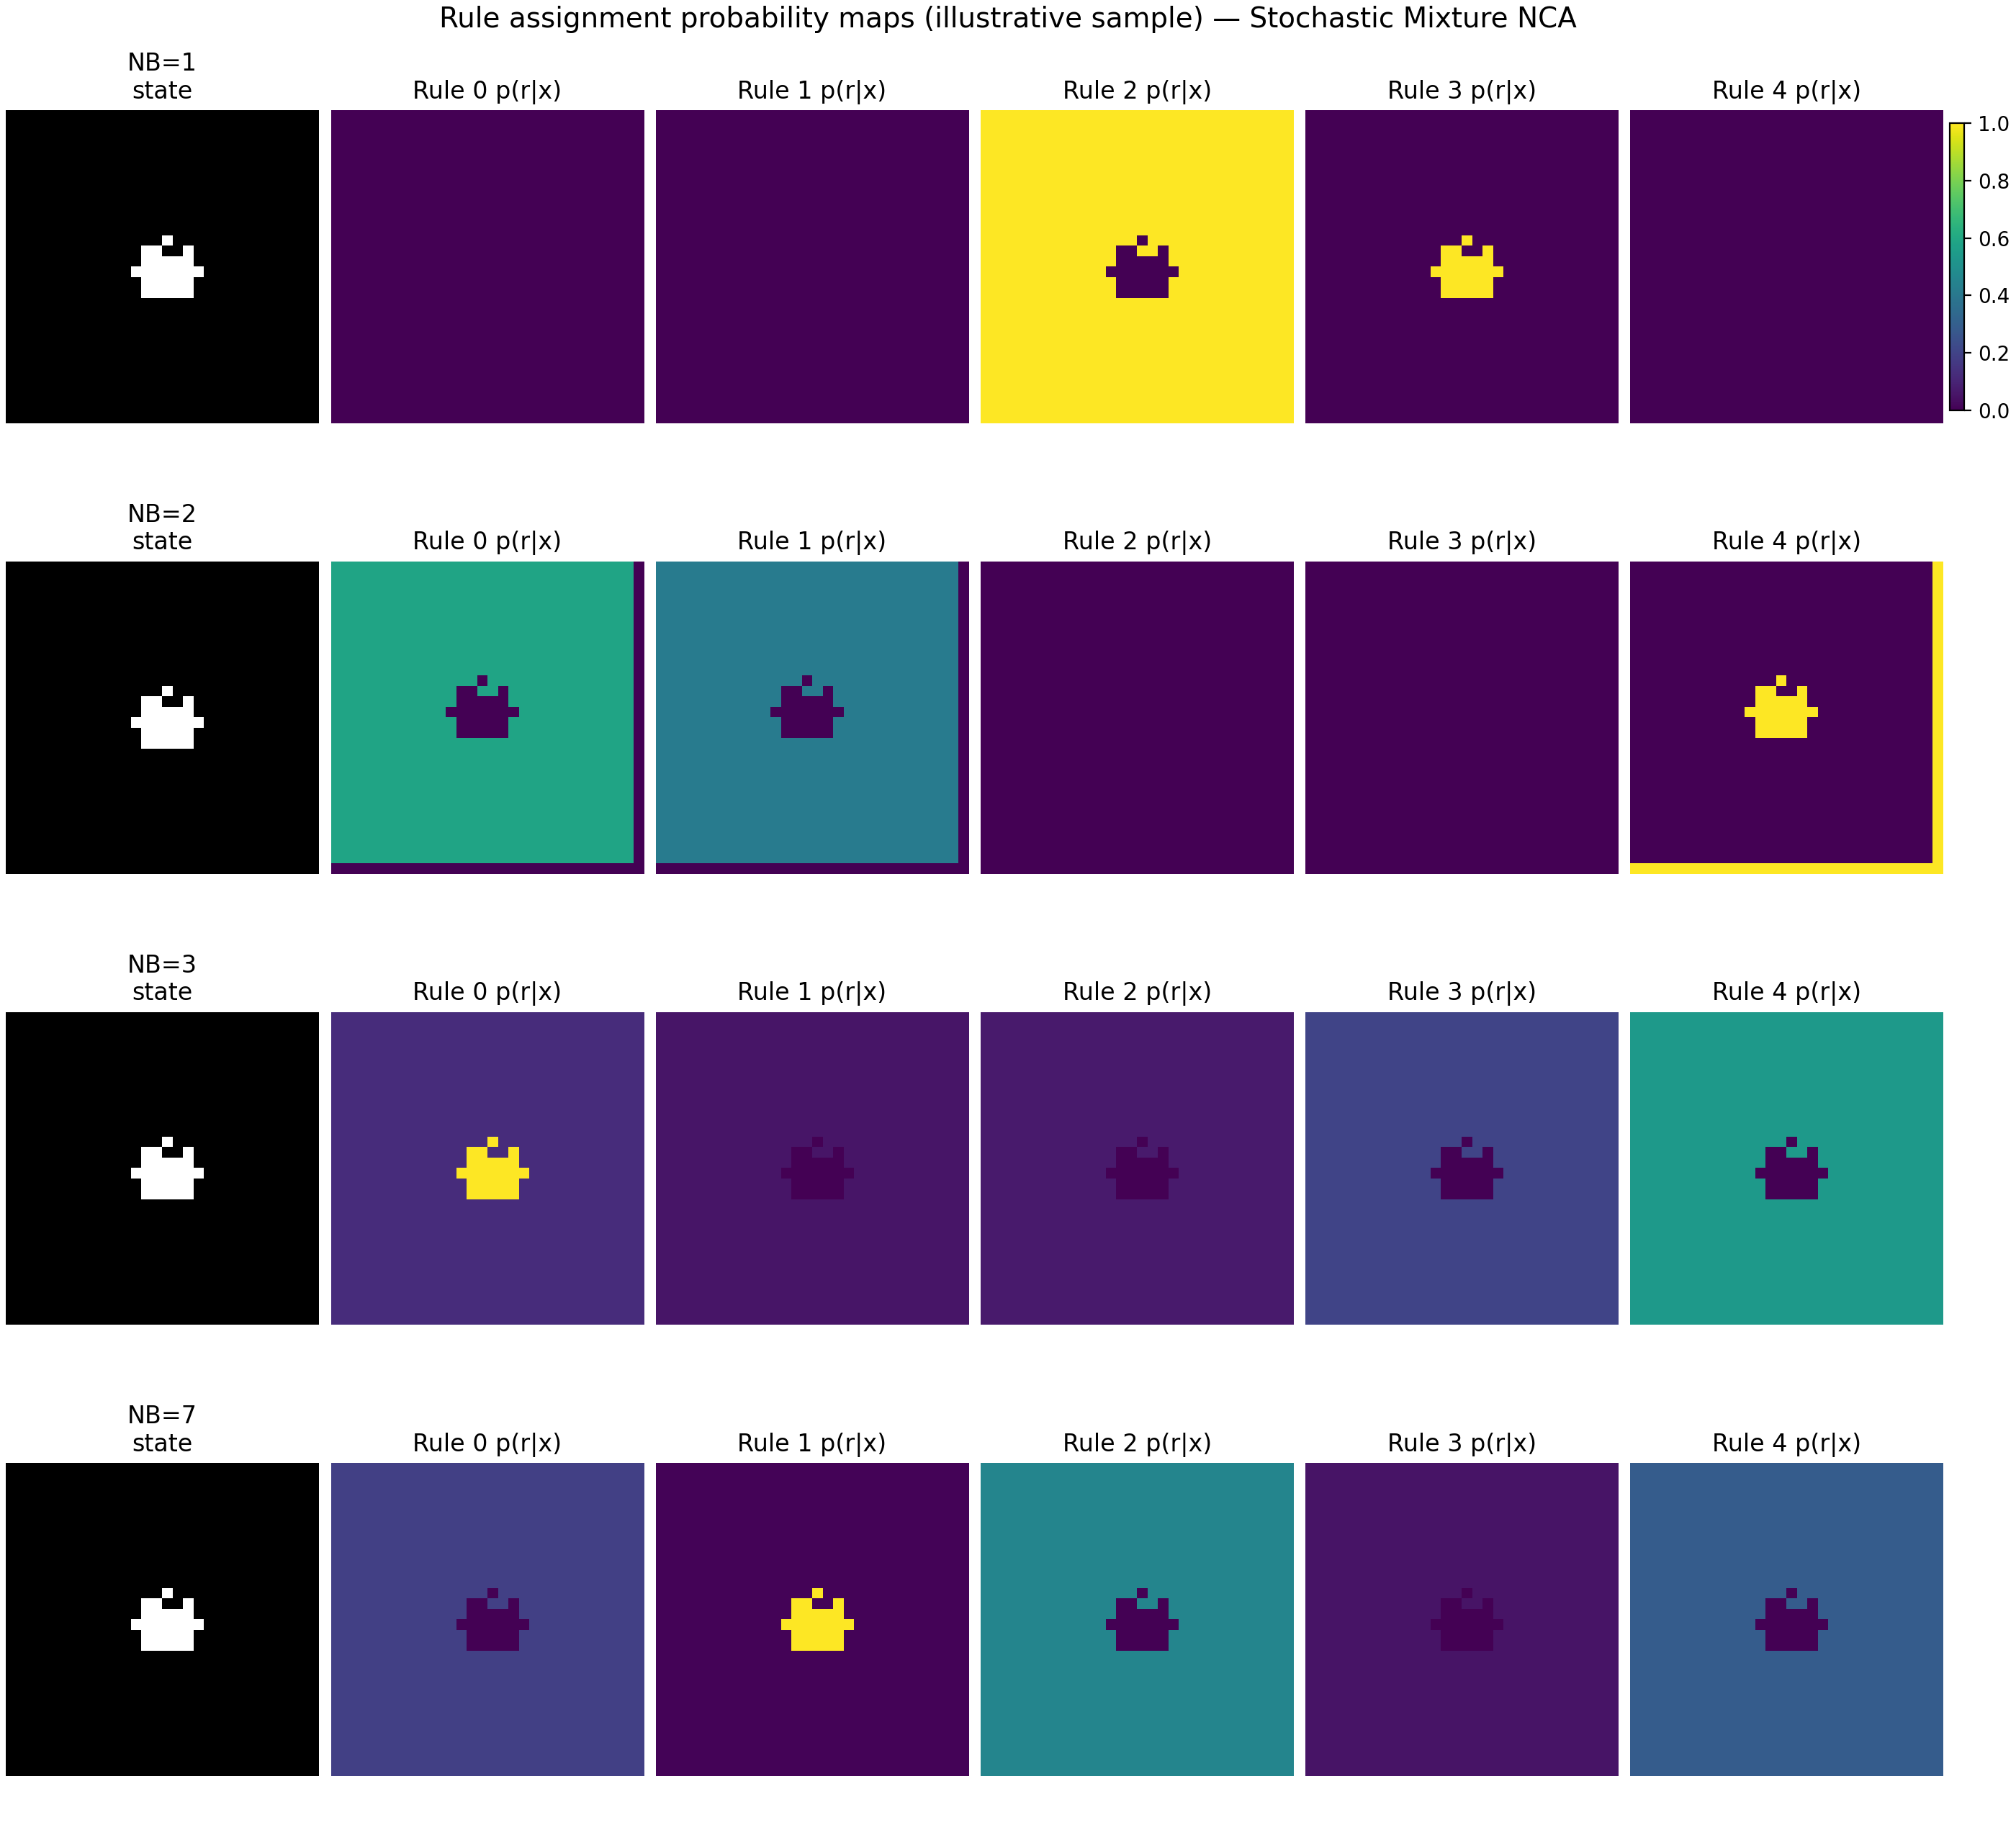
\includegraphics[width=\textwidth]{figs/neighborhood_analysis/nb_sweep_300x100/rule_assignment_maps_stochastic.png}
  \caption{Step 3: rule assignment probability maps for Stochastic Mixture NCA (one example state). \textbf{Legend:} same layout as Figure~\ref{fig:impl:step3:rule:maps:mix} (columns = state + five rule maps, rows = \(NB\); colour = probability).}
  \label{fig:impl:step3:rule:maps:stoch}
\end{figure}

\subsubsection{Statistical tests across neighbourhood sizes}
\label{sec:results:step3:stats}

% Auto-generated by experiments/generate_step3_stats_table.py
% Statistical tests: Step Length=100, baselines NB=2 and NB=3, Holm correction.
\begin{table}[H]
\centering
\small
\begin{tabulary}{\textwidth}{lLrLL}
\toprule
Model & Metric & Kruskal-Wallis $p$ & Significant vs NB=2 & Significant vs NB=3 \\
\midrule
Mixture~NCA & KL Divergence & $<10^{-4}$ & 3,4,5,6,7 & 4,5,6,7 \\
Mixture~NCA & Chi-Square & $<10^{-4}$ & 3,4,5,6,7 & 4,5,6,7 \\
Mixture~NCA & Categorical MMD & $<10^{-4}$ & 3,4,5,6,7 & 4,5,6 \\
Mixture~NCA & Tumour Size Diff & $<10^{-4}$ & 3,4,5,6,7 & 4,5,6,7 \\
Mixture~NCA & Border Size Diff & $<10^{-4}$ & 3,4,5,6,7 & 4,5,6,7 \\
Mixture~NCA & Spatial Variance Diff & $<10^{-4}$ & 3,4,5,6,7 & 4,5,6,7 \\
Stochastic~Mixture~NCA & KL Divergence & $<10^{-4}$ & 3,4,5,6,7 & 4,5,6,7 \\
Stochastic~Mixture~NCA & Chi-Square & $<10^{-4}$ & 3,4,5,6,7 & 4,5,6,7 \\
Stochastic~Mixture~NCA & Categorical MMD & $<10^{-4}$ & 3,4,5,7 & 4,5,6,7 \\
Stochastic~Mixture~NCA & Tumour Size Diff & $<10^{-4}$ & 3,4,5,7 & 4,5,6,7 \\
Stochastic~Mixture~NCA & Border Size Diff & $<10^{-4}$ & 4,5,6,7 & 4,5,6,7 \\
Stochastic~Mixture~NCA & Spatial Variance Diff & $<10^{-4}$ & 3,4,5,6,7 & 4,5,7 \\
\bottomrule
\end{tabulary}
\caption{Non-parametric statistical tests across neighbourhood sizes for Step Length $=100$. \textbf{Legend:} Model = Mixture NCA or Stochastic Mixture NCA; Metric = one of the six metrics; Kruskal-Wallis $p$ over $NB\in\{1,\dots,7\}$; last two columns = list of $NB$ that differ significantly from baseline $NB=2$ (post-hoc Mann-Whitney U, Holm correction) and from baseline $NB=3$.}
\label{tab:impl:step3:stats}
\end{table}


\paragraph{Interpretation and comparison of the two baselines.}
The Kruskal-Wallis \(p\)-values are below \(10^{-4}\) for all metrics and both models, so we have strong evidence that neighbourhood size affects the distribution of each metric.
Comparing the two baseline columns reinforces and refines this conclusion.

\emph{Vs.\ \(NB=2\):} For the Mixture model, every metric lists \(NB=3,4,5,6,7\) as significant (i.e.\ even the first step beyond the minimum (\(NB=3\)) is distinguishable from \(NB=2\)).
For the Stochastic model, the same holds for most metrics; exceptions are Border Size Diff (only \(4,5,6,7\): \(NB=3\) is not significantly different from \(NB=2\)) and, for Categorical MMD and Tumor Size Diff, \(NB=6\) is not in the significant set, so for those metrics \(NB=6\) is not clearly better than \(NB=2\).

\emph{Vs.\ \(NB=3\):} Here we only compare \(NB=4,5,6,7\) to \(NB=3\), so the column never contains 3.
For the Mixture model, Categorical MMD gives only \(4,5,6\) (so \(NB=7\) is not significantly different from \(NB=3\) for that metric); for all other metrics, \(4,5,6,7\) are significant vs.\ \(NB=3\).
For the Stochastic model, Spatial Variance Diff gives only \(4,5,7\) (so \(NB=6\) is not significantly different from \(NB=3\)), while Categorical MMD and Tumor Size Diff list \(4,5,6,7\) and Border Size Diff \(4,5,6,7\).

\emph{Takeaway:} The two baselines tell a consistent story: the effect of \(NB\) is statistically significant and not due to noise; going from \(NB=2\) to \(NB=3\) often (but not always, e.g.\ Stochastic Border Size) matters; beyond \(NB=3\), which of \(NB=4,5,6,7\) differ from the reference depends on the metric and the model.
So the ``best'' neighbourhood size is metric- and model-dependent, and the tests with both baselines support the same overall message while making the dependence on the reference explicit.

%-------------------------------------------------------------------
\section{Role of stochasticity and long-horizon rollouts}
\label{sec:results:stochasticity}
%-------------------------------------------------------------------

A key qualitative and quantitative conclusion is that the \textbf{stochastic MNCA variant} tends to be more reliable for \textbf{long-horizon tissue-like behaviour}, particularly when evaluation is performed as \textbf{free rollout} (i.e., the model evolves without being corrected by ground-truth states).
This is important because the thesis explicitly treats free rollout as the meaningful deployment regime: it exposes drift and compounding errors that teacher forcing can hide.

In the curriculum learning experiment (\cref{sec:impl:curriculum}, trained on progressively longer temporal windows and evaluated at 25, 100, and 500 steps), the results clarify the following:
\begin{itemize}
\item For \textbf{distributional metrics} (KL divergence, Chi-square, categorical MMD), \textbf{Stochastic Mixture NCA} consistently outperforms the deterministic Mixture NCA, and the advantage becomes more evident at longer horizons.
\item In particular, categorical MMD shows a strong neighbourhood dependence at long rollout lengths: at 100 and 500 steps, the stochastic model improves as neighbourhood size increases within the tested set (\(NB\in\{2,3,5\}\)), reaching \textbf{values around 0.04 to 0.05 at \(NB=5\)}.
\item For \textbf{spatial metrics} (tumour size difference, border size difference, spatial variance difference), the behaviour is more nuanced: deterministic Mixture NCA can be competitive (or even best) at intermediate neighbourhoods for structural sharpness, whereas the stochastic model can show an intermediate ``peak'' in error (notably around \(NB=3\)) before recovering at larger neighbourhoods (e.g., \(NB=5\)).
\end{itemize}

Overall, the curriculum experiment supports the idea that \textbf{stochasticity plus sufficient spatial context} can improve \emph{global} fidelity and reduce runaway dynamics at long time scales, while fine-grained geometric fidelity may require careful balancing between randomness and receptive field size.

\subsection{Curriculum experiment: qualitative behaviour and metric trends}
\label{sec:results:curriculum}
%-------------------------------------------------------------------

To see how the curriculum-trained models behave in practice, we pick \textbf{three simulations} (Sim~0, Sim~149, Sim~299) and compare the ground truth with the Mixture NCA and the Stochastic Mixture NCA for \(NB=2\), \(NB=3\), and \(NB=5\) at four time points: \(t=10\), \(t=50\), \(t=100\), and \(t=500\).
For each neighbourhood size we show three rows (ground truth, Mixture NCA, Stochastic Mixture NCA) and four columns (one per time point); the layout is split by \(NB\) (Figures~\ref{fig:impl:curriculum:ex_nb2} to \ref{fig:impl:curriculum:ex_nb5}).
The same initial state is used per simulation for all three rows, so the comparison is fair.

\paragraph{Ground truth.}
The simulator produces robust, organic growth: small clusters at \(t=10\) expand into intricate, irregular or branching structures by \(t=500\), with clear boundaries between cell types and controlled, localized growth that does not fill the grid.

\paragraph{Mixture NCA (deterministic).}
At \(t=10\) the Mixture NCA often resembles the ground truth, in line with the first curriculum phase (35-step windows).
From \(t=50\) onward, however, it diverges sharply: it exhibits \emph{aggressive, uncontrolled expansion}, rapidly filling a large portion of the grid with blocky, often homogeneous regions (dominantly green and purple), and loses the fine internal structure and sharp boundaries of the ground truth.
This behaviour is consistent across \(NB=2\), \(NB=3\), and \(NB=5\): the deterministic mixture fails to maintain localized complexity and instead tends toward large-scale, artificial-looking growth.

\paragraph{Stochastic Mixture NCA.}
At \(t=10\) the stochastic variant also tracks the ground truth well.
Over time it performs \emph{noticeably better} than the deterministic Mixture NCA: it keeps the overall scale and footprint of the patterns closer to the ground truth, avoids the runaway expansion, and preserves more organic shapes and irregular boundaries.
For \(NB=3\) and \(NB=5\) (Figures~\ref{fig:impl:curriculum:ex_nb3} to \ref{fig:impl:curriculum:ex_nb5}), the qualitative agreement with the ground truth at \(t=50\), \(t=100\), and \(t=500\) is strong: growth remains controlled and morphologies are close to the target.
For \(NB=2\) (Figure~\ref{fig:impl:curriculum:ex_nb2}), stochasticity still improves containment and scale, but the internal structure can appear noisier or less sharply defined than the ground truth, and fine-grained cell-type segregation is only partly reproduced.
In summary, the stochastic component is crucial for stable, morphologically plausible long-horizon behaviour and aligns with the better distributional metrics we report for the stochastic model at larger \(NB\) and longer step lengths.

\begin{figure}[H]
  \centering
  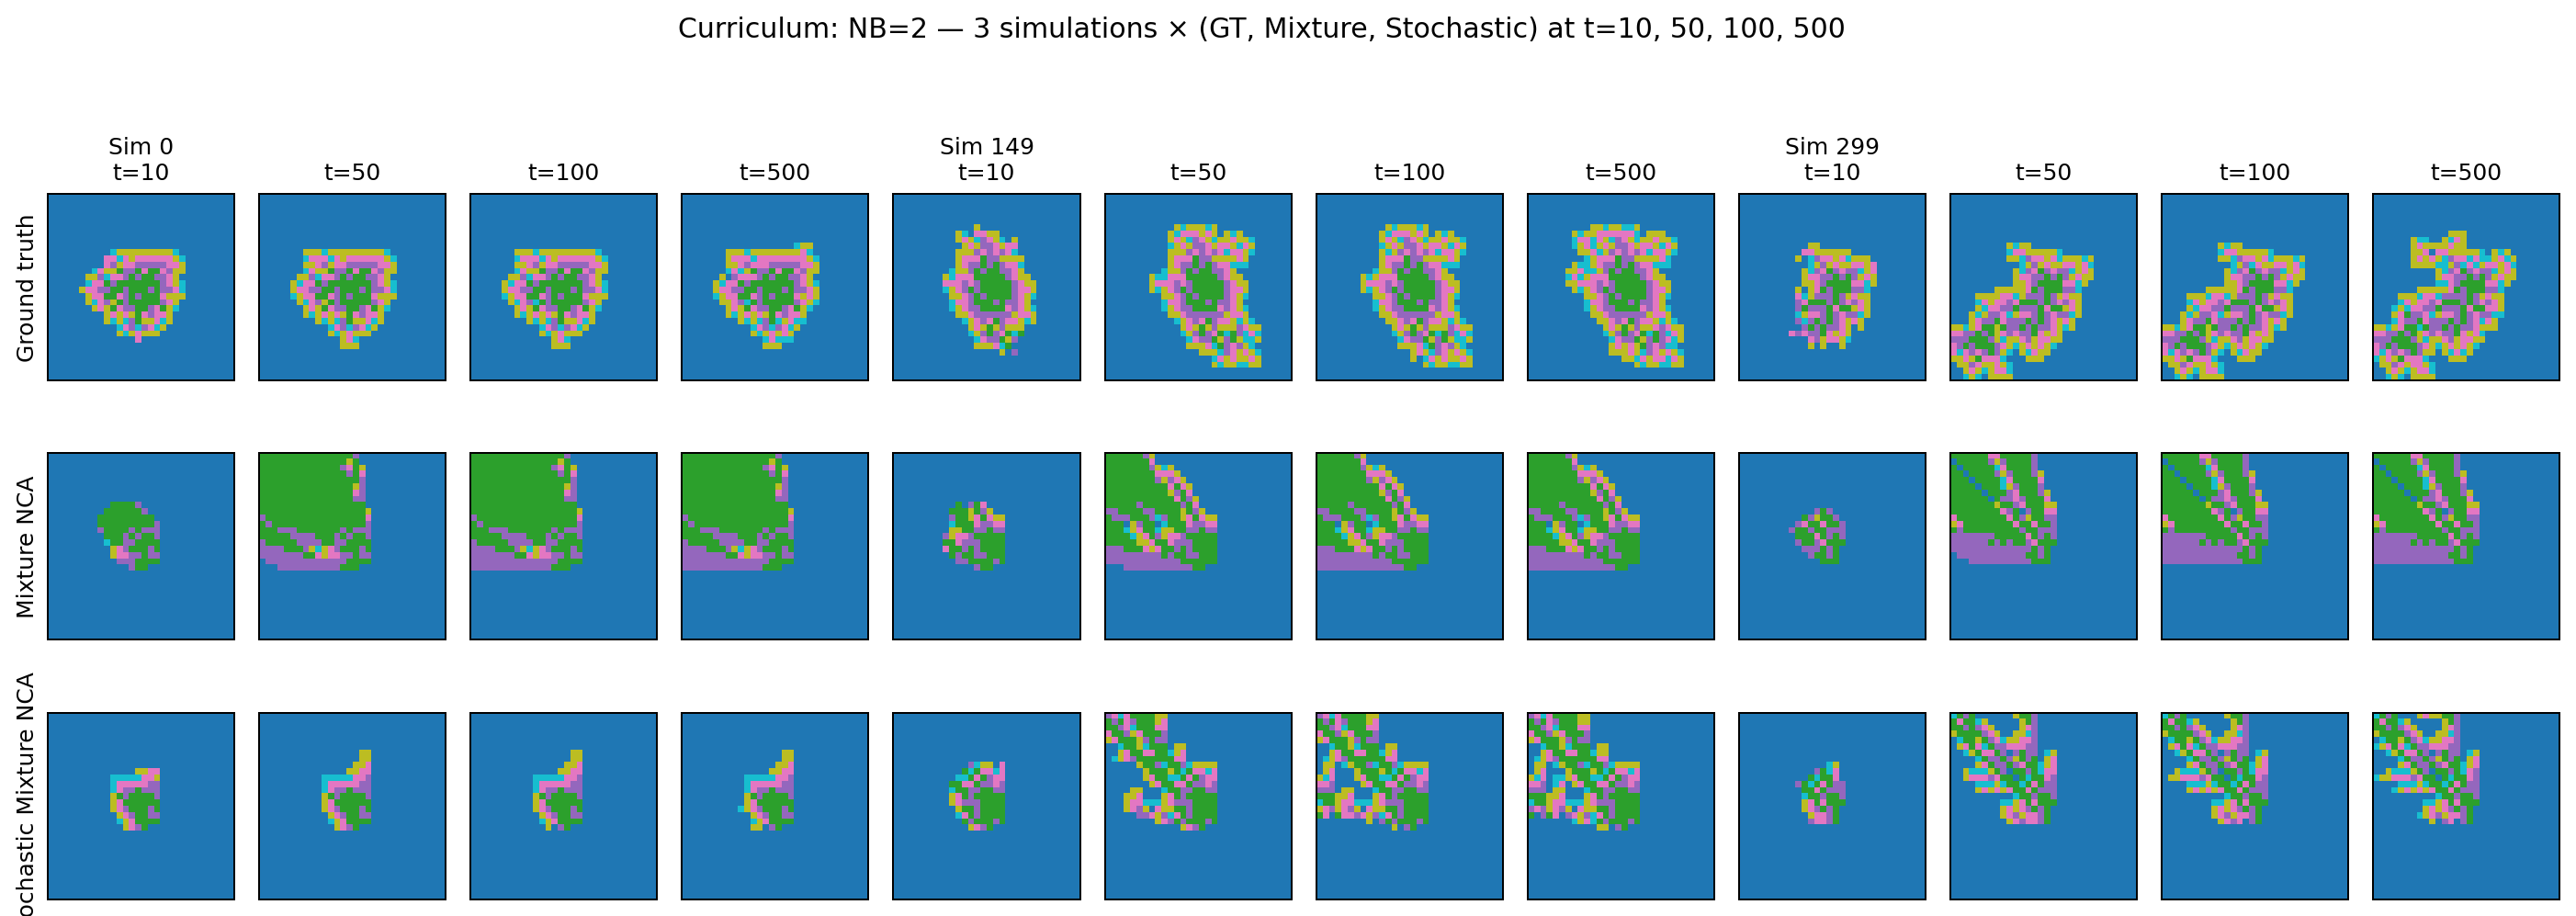
\includegraphics[width=\textwidth]{figs/curriculum/curriculum_examples_NB2.png}
  \caption{Curriculum experiment, \(NB=2\). \textbf{Legend:} three rows = ground truth, Mixture NCA, Stochastic Mixture NCA; four columns = time steps \(t=10,50,100,500\); each block = one of three simulations (same initial state for all three rows).}
  \label{fig:impl:curriculum:ex_nb2}
\end{figure}

\begin{figure}[H]
  \centering
  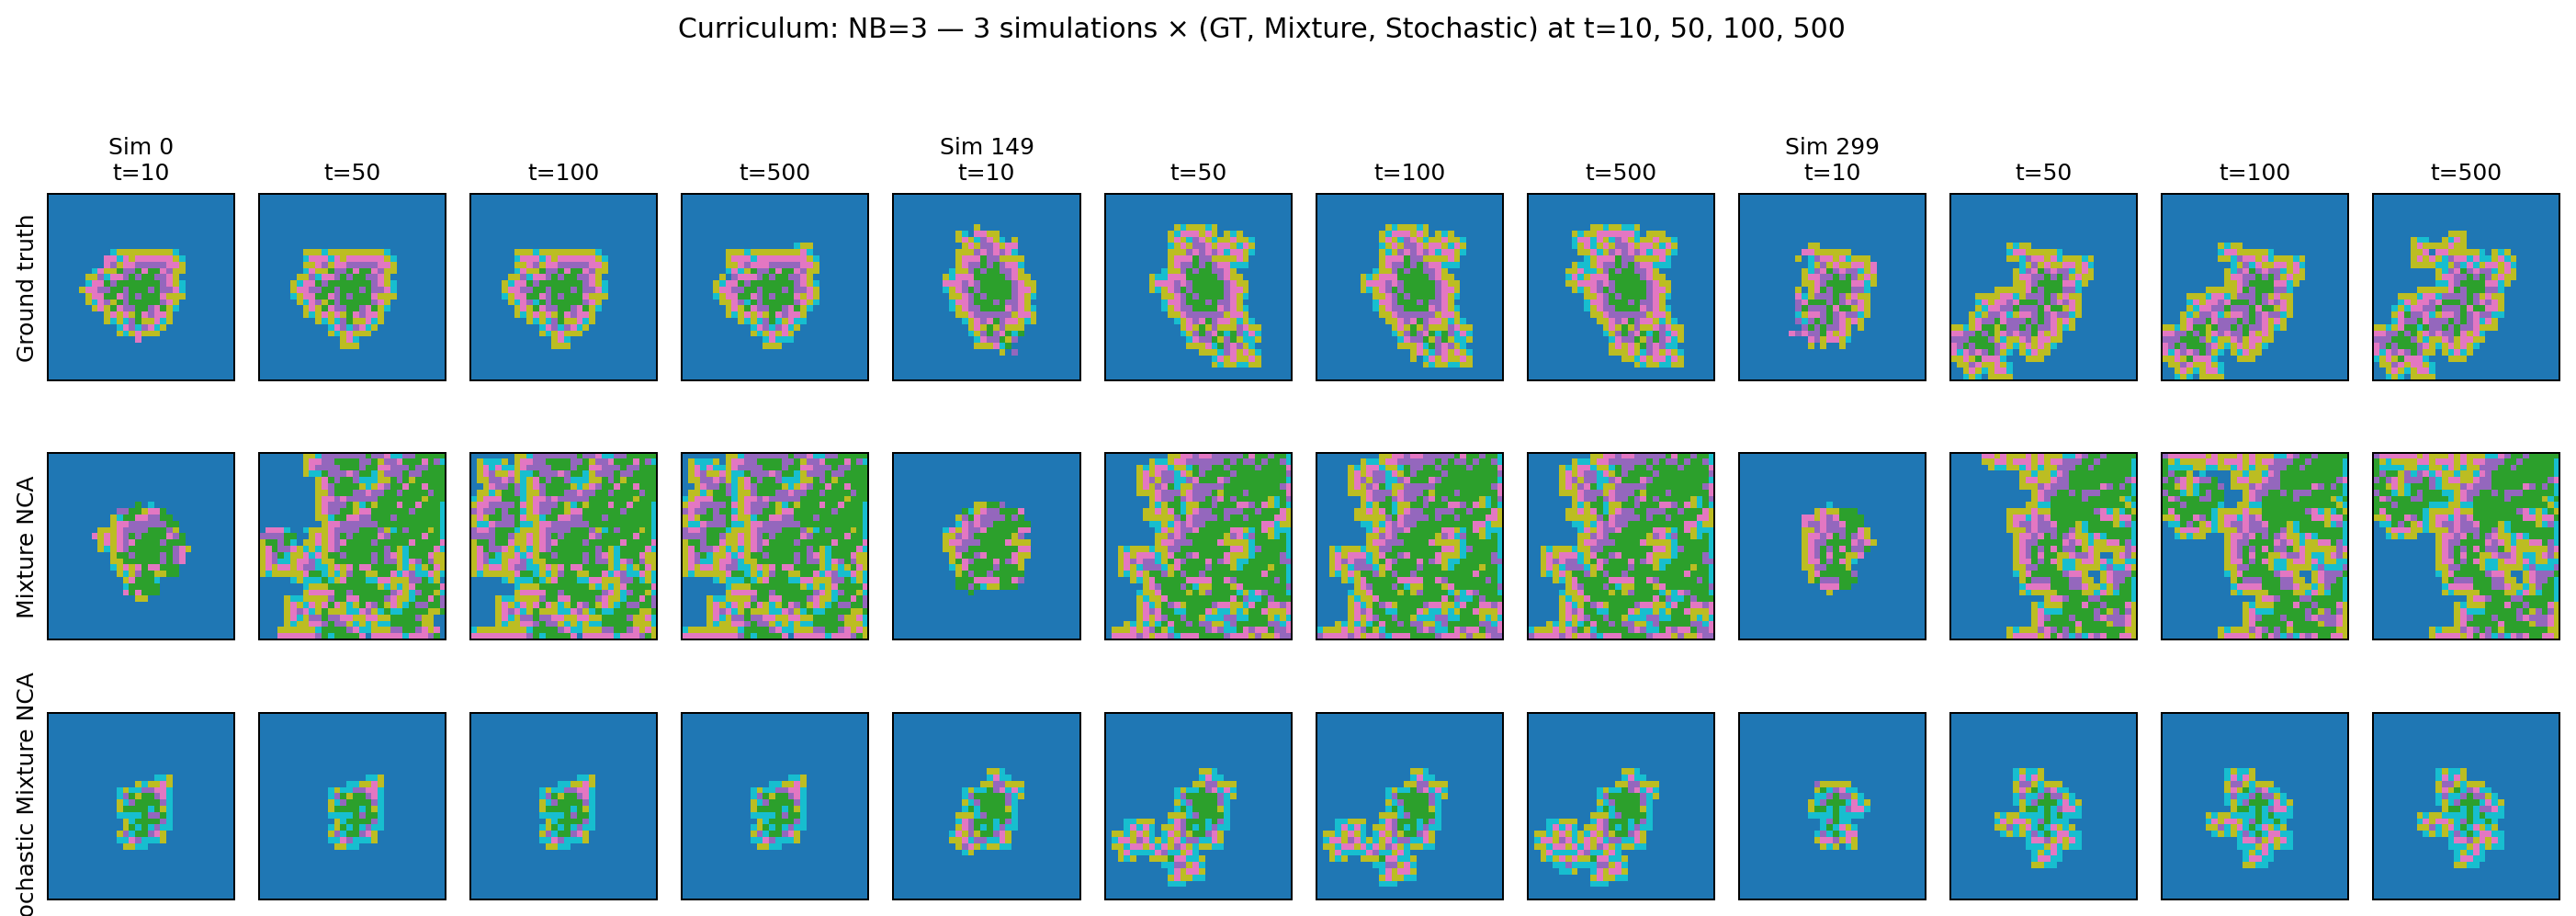
\includegraphics[width=\textwidth]{figs/curriculum/curriculum_examples_NB3.png}
  \caption{Curriculum experiment, \(NB=3\). \textbf{Legend:} same as Figure~\ref{fig:impl:curriculum:ex_nb2} (rows = GT, Mixture NCA, Stochastic; columns = \(t=10,50,100,500\); three simulations).}
  \label{fig:impl:curriculum:ex_nb3}
\end{figure}

\begin{figure}[H]
  \centering
  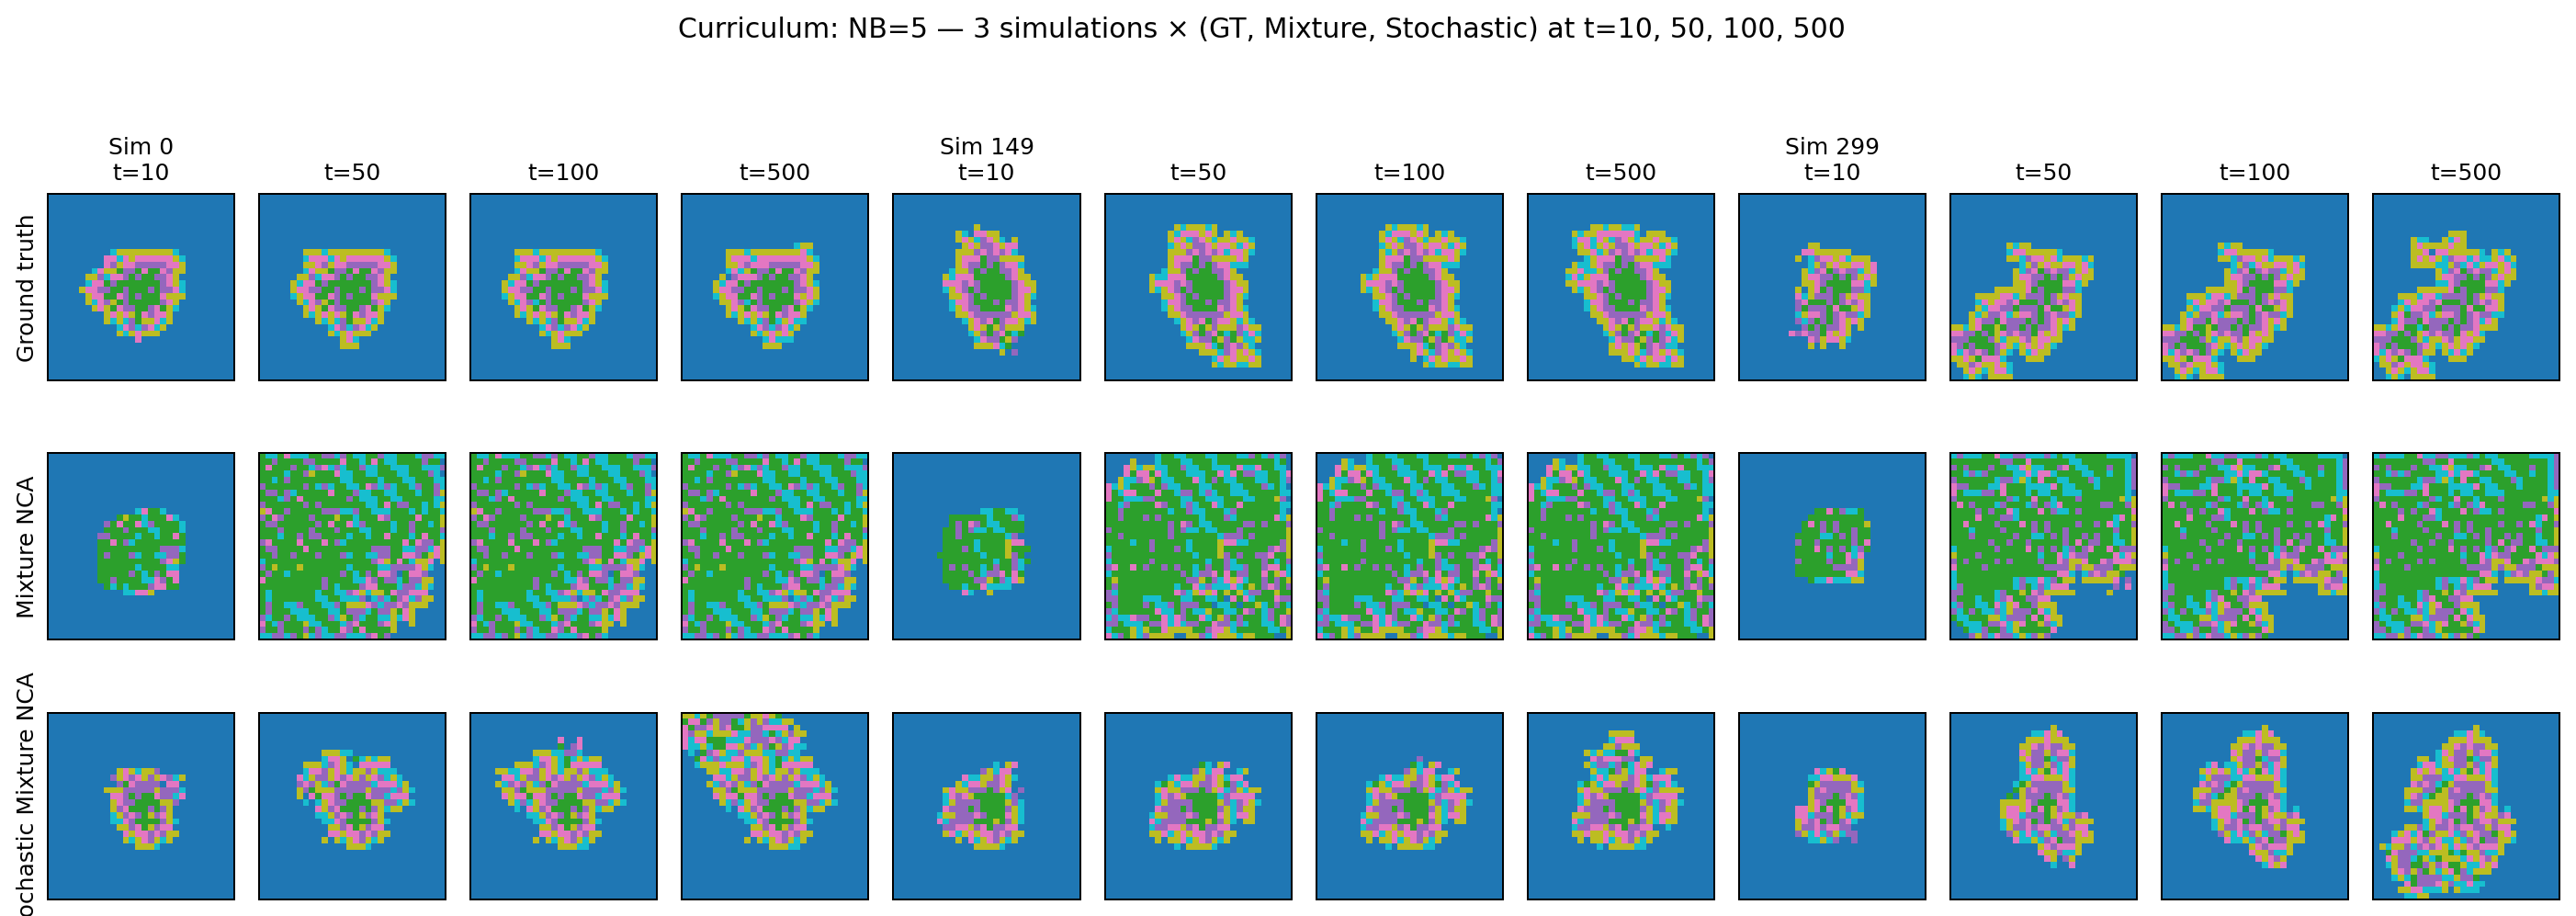
\includegraphics[width=\textwidth]{figs/curriculum/curriculum_examples_NB5.png}
  \caption{Curriculum experiment, \(NB=5\). \textbf{Legend:} same as Figure~\ref{fig:impl:curriculum:ex_nb2} (rows = GT, Mixture NCA, Stochastic; columns = \(t=10,50,100,500\); three simulations).}
  \label{fig:impl:curriculum:ex_nb5}
\end{figure}

\subsubsection{Metric results and interpretation}
\label{sec:results:curriculum:metrics}

After training we run the evaluation protocol (free rollouts at 25, 100, and 500 steps) for each combination of neighbourhood size and step length, and we record the six biological metrics.
Figure~\ref{fig:impl:curriculum:dashboard} reports the \emph{mean} of each metric over the three step lengths (25, 100, 500) for each neighbourhood size and each model; Table~\ref{tab:impl:curriculum:metrics_summary} summarises which configuration is best per metric and explains the contrast between metric types.

\paragraph{Distributional metrics (KL divergence, Chi-square, categorical MMD).}
These metrics measure how closely the \emph{global statistical distribution} of cell states (or derived counts) in the generated pattern matches the ground truth (e.g., proportions of cell types, overall composition).
On all three, \textbf{Stochastic Mixture NCA} clearly outperforms Mixture NCA, and the gap widens as \(NB\) increases: at \(NB=5\) the stochastic model attains the lowest values (e.g., KL and Chi-square roughly halved or better vs.\ the deterministic one; categorical MMD much lower at \(NB=5\)).
The deterministic Mixture NCA improves from \(NB=2\) to \(NB=3\) but then plateaus or slightly degrades (e.g., Chi-square and categorical MMD rise again from \(NB=3\) to \(NB=5\)), as if the larger receptive field does not help it further for distributional fidelity.
The stochastic variant, by contrast, benefits consistently from a larger neighbourhood: it can explore the state space more and, with more context, better approximate the target distribution.

\paragraph{Spatial metrics (tumour size diff, border size diff, spatial variance diff).}
These metrics measure \emph{geometric and structural} accuracy: size of the active region, extent of boundaries, and spatial clustering or dispersion.
Here the picture is more nuanced and the two models behave differently.
\textbf{Mixture NCA} often performs best at \textbf{\(NB=3\)} for border size and spatial variance: the deterministic rule, with a moderate neighbourhood, can form stable local structures and sharp boundaries without the extra variability that stochasticity introduces.
\textbf{Stochastic Mixture NCA} exhibits a pronounced \emph{peak in error at \(NB=3\)} on border size and spatial variance (worse than at \(NB=2\) or \(NB=5\)), suggesting that at this scale the randomness interferes with precise spatial coherence.
At \textbf{\(NB=5\)}, the stochastic model recovers: it improves on tumour size diff, border size diff, and spatial variance diff, and at \(NB=5\) often matches or beats the deterministic model on these spatial metrics, while the deterministic one can degrade (e.g., spatial variance diff rises from \(NB=3\) to \(NB=5\)).
At \(NB=2\), Mixture NCA sometimes has an edge on spatial metrics (e.g., tumour size diff), but both models are less stable at long horizons when \(NB\) is small.

\paragraph{Why distributional and spatial metrics give different results.}
Distributional metrics aggregate over the whole pattern and reward a good match of \emph{overall} counts and proportions; they benefit from the stochastic model's ability to explore and from a larger receptive field (\(NB=5\)), which provides more context for consistent long-horizon behaviour.
Spatial metrics, in contrast, are sensitive to \emph{local} geometry: sharp borders, coherent regions, and stable spatial arrangement.
Stochasticity can help globally but add local ``noise'' or blurring, which hurts border and spatial-variance accuracy at an intermediate scale (\(NB=3\)); the deterministic model, with no sampling noise, can excel at that scale for structure.
When \(NB\) is increased to 5, the stochastic model gains enough context to stabilise its spatial behaviour (or the randomness averages out better), so it recovers and often surpasses the deterministic one even on spatial metrics.
Hence there is no single ``best'' \(NB\) or model for all metrics: the choice depends on whether one prioritises distributional agreement (favor Stochastic Mixture NCA and \(NB=5\)) or fine-grained spatial fidelity at a given scale (where \(NB=3\) can be best for the deterministic model, and \(NB=5\) for the stochastic one).

\paragraph{How the metrics change with step length.}
We evaluate at 25, 100, and 500 steps to see how performance changes as the rollout gets longer.
At \textbf{25 steps} we are close to what the model saw in the first curriculum phase (35-step windows), so errors stay low and the difference between \(NB=2\), \(NB=3\), and \(NB=5\) is small.
At \textbf{100} and \textbf{500 steps} the metrics generally worsen and the receptive field matters more: distributional metrics are clearly best for \(NB=5\), especially for the stochastic model; spatial metrics show the trade-offs described above (e.g., Mixture NCA best at \(NB=3\) for some, Stochastic best at \(NB=5\) after recovering from the \(NB=3\) peak).
Figure~\ref{fig:impl:curriculum:categorical_mmd} breaks out categorical MMD by step length; the dashboard (Figure~\ref{fig:impl:curriculum:dashboard}) averages over step lengths and gives the overall picture.

\paragraph{Comparison with Step 3.}
In Step 3 we had 300 trajectories of 100 steps, no curriculum, and we evaluated at 25, 50, and 100 steps with \(NB\) from 1 to 7.
Here we have 300 trajectories of 500 steps, a three-phase curriculum (35, 100, 500), and we evaluate at 25, 100, and 500 steps with \(NB \in \{2,3,5\}\).
The conclusions match: in both experiments, larger neighbourhoods help on distributional metrics at longer horizons, and no single \(NB\) is best on every metric.
Step 3 showed that \(NB=1\) is too small and that \(NB\ge2\) gives a clear improvement; this curriculum run shows that among 2, 3, and 5, the larger one (\(NB=5\)) is better at 100 and 500 steps, especially for the stochastic model.
We use the same six metrics in both experiments, so the comparison is fair; the curriculum experiment simply pushes the evaluation horizon to 500 steps and confirms that the neighbourhood-size effect is still there.

\begin{figure}[H]
  \centering
  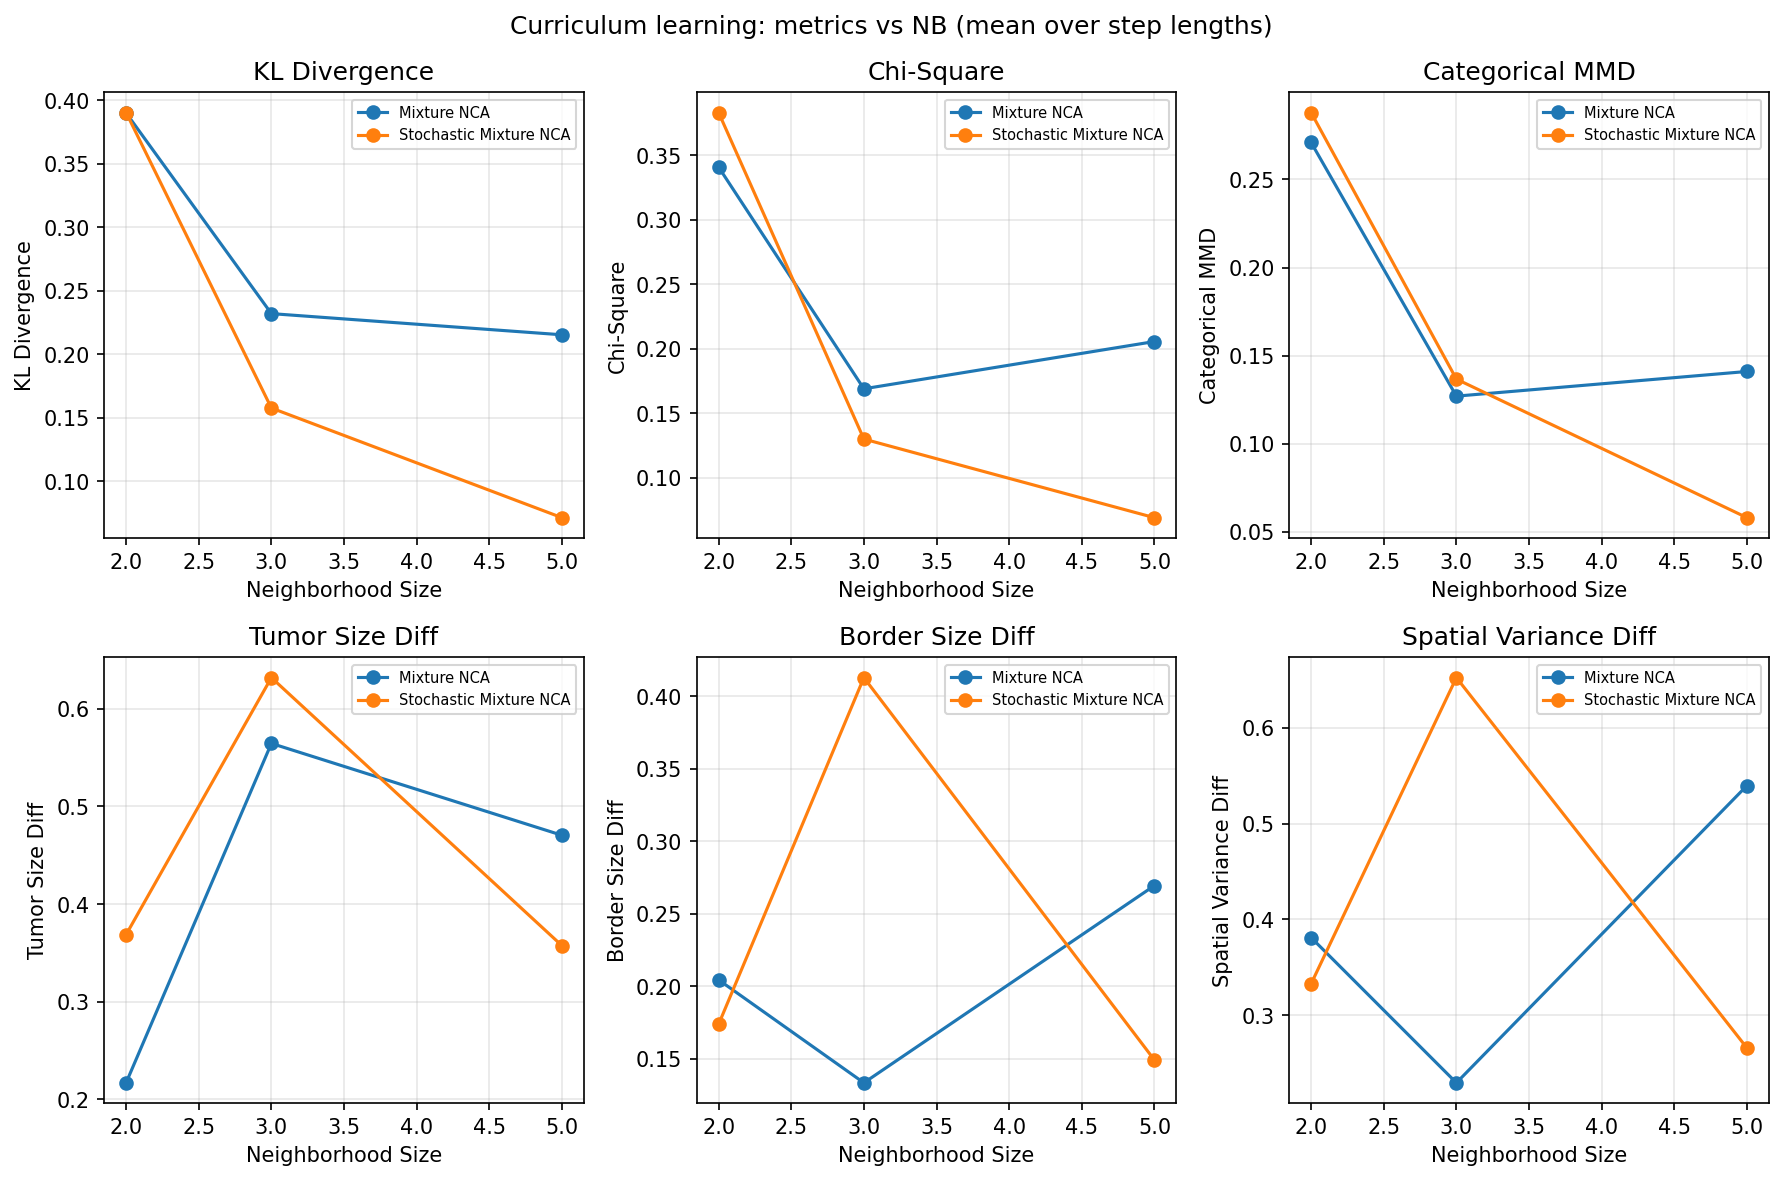
\includegraphics[width=\textwidth]{figs/curriculum/curriculum_dashboard.png}
  \caption{Curriculum experiment: mean metric values vs.\ neighbourhood size. \textbf{Legend:} six panels = KL divergence, Chi-square, categorical MMD (top), tumour size diff, border size diff, spatial variance diff (bottom); abscissa = \(NB\); ordinate = mean over step lengths 25, 100, 500 (lower is better); series = Mixture vs.\ Stochastic Mixture NCA.}
  \label{fig:impl:curriculum:dashboard}
\end{figure}

% Summary of curriculum experiment: best configuration per metric (mean over step lengths 25, 100, 500)
\begin{table}[H]
\centering
\small
\begin{tabulary}{\textwidth}{lLLL}
\toprule
Metric & Type & Mixture NCA (best \(NB\)) & Stochastic Mixture NCA (best \(NB\)) \\
\midrule
KL Divergence & Distributional & \(NB=5\) (plateau after \(NB=3\)) & \(NB=5\) (lowest; large gain vs.\ det.) \\
Chi-Square & Distributional & \(NB=3\) (degrades at \(NB=5\)) & \(NB=5\) (lowest) \\
Categorical MMD & Distributional & \(NB=3\) (slight rise at \(NB=5\)) & \(NB=5\) (lowest) \\
\midrule
Tumor Size Diff & Spatial & \(NB=2\) (peaks at \(NB=3\)) & \(NB=5\) (recovers after \(NB=3\) peak) \\
Border Size Diff & Spatial & \(NB=3\) (best) & \(NB=5\) (poor at \(NB=3\), then recovers) \\
Spatial Variance Diff & Spatial & \(NB=3\) (best; worsens at \(NB=5\)) & \(NB=5\) (peak at \(NB=3\), then best) \\
\bottomrule
\end{tabulary}
\caption{Curriculum experiment: summary of which neighborhood size yields the best mean value (over step lengths 25, 100, 500) for each metric and model. ``Type'' distinguishes distributional (global statistics) vs.\ spatial (geometry/structure). The deterministic model often peaks at \(NB=3\) on spatial metrics; the stochastic model peaks in error at \(NB=3\) on spatial metrics then improves at \(NB=5\).}
\label{tab:impl:curriculum:metrics_summary}
\end{table}


\paragraph{Why we see these values.}
The model is trained on windows of 35, 100, and 500 steps, so it learns to match the data over longer and longer horizons.
But at evaluation we use free rollouts: the model has to stay coherent for 25, 100, or 500 steps without ever seeing the true state again after the start.
Short rollouts (25 steps) are close to the first training phase, so all three neighbourhood sizes do well and the gap between them is small.

When we go to 100 and 500 steps, errors build up and the receptive field matters more: a larger neighbourhood (\(NB=5\)) gives the update rule more context, which helps keep the tissue consistent (hence better KL and Chi-square) and, for the stochastic model, keeps rule choices more stable over time (hence the clearer win for \(NB=5\) at long horizons).
The deterministic Mixture NCA mixes rules in a soft way, so it is less sensitive to sampling noise but can still drift over long rollouts; depending on the metric and the horizon, we sometimes see \(NB=3\) best for border or spatial variance and \(NB=5\) best for KL and categorical MMD.

Figure~\ref{fig:impl:curriculum:categorical_mmd} zooms in on categorical MMD as we change neighbourhood size and step length.
At \textbf{25 steps} both models achieve low MMD for all \(NB\); the curve is often U-shaped with a minimum at \(NB=3\) for Mixture NCA, and similar for the stochastic variant.
At \textbf{100} and \textbf{500 steps} the two models diverge: \textbf{Stochastic Mixture NCA} shows a monotonic decrease in MMD as \(NB\) increases, reaching the lowest values at \(NB=5\) (around 0.04 to 0.05), whereas \textbf{Mixture NCA} again exhibits a U-shaped trend with minimum at \(NB=3\) and a rise at \(NB=5\) (especially at 500 steps).
So for this distributional metric at long horizons, the stochastic model benefits consistently from a larger receptive field, while the deterministic one does not improve beyond \(NB=3\) and can even degrade. This is consistent with the dashboard and with the interpretation that stochasticity plus context (\(NB=5\)) yields better global distributional match.

\begin{figure}[H]
  \centering
  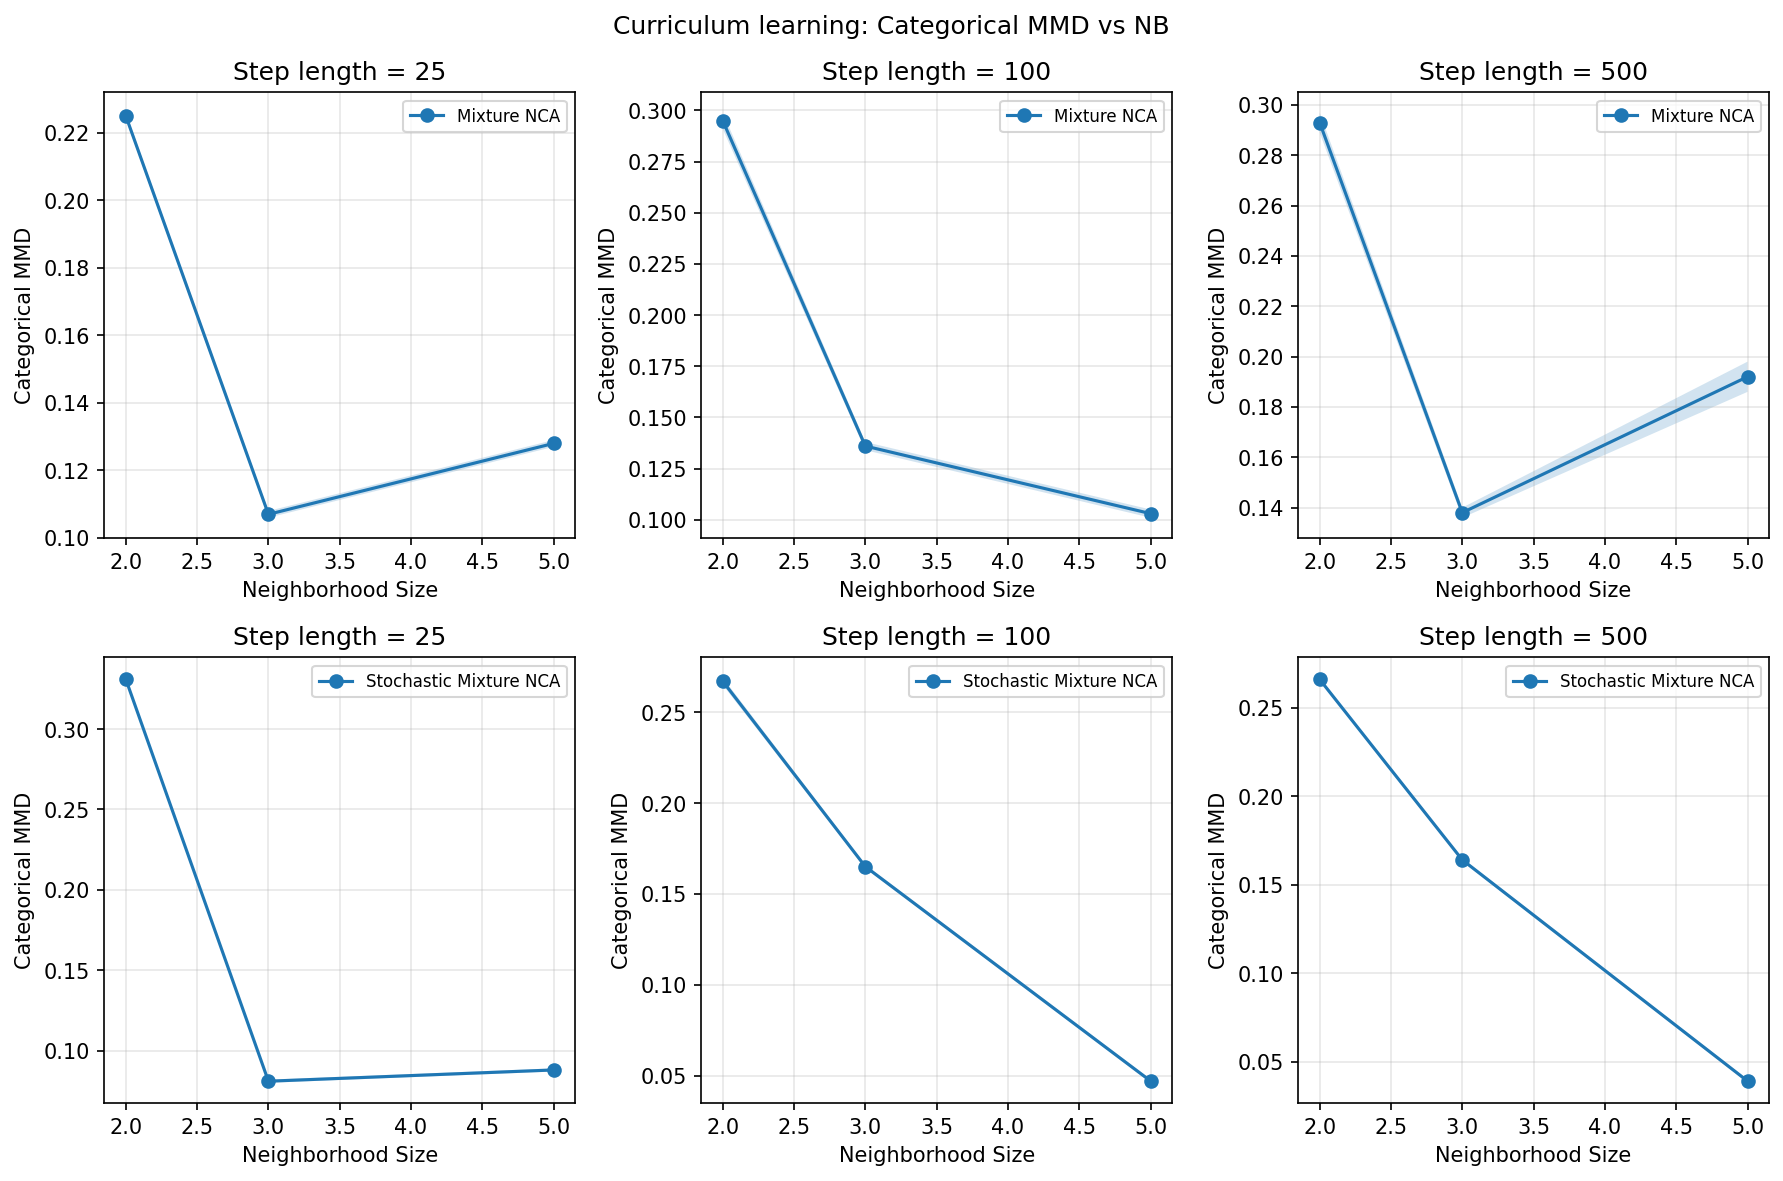
\includegraphics[width=\textwidth]{figs/curriculum/curriculum_metric_vs_nb_categorical_mmd.png}
  \caption{Curriculum experiment: categorical MMD vs.\ neighbourhood size. \textbf{Legend:} columns = step length (25, 100, 500); top row = Mixture NCA, bottom row = Stochastic Mixture NCA; abscissa = \(NB\), ordinate = categorical MMD (lower is better).}
  \label{fig:impl:curriculum:categorical_mmd}
\end{figure}

The training loss curves (Figure~\ref{fig:impl:curriculum:loss}) show that both models converge quickly: on a linear scale the loss drops to values near zero within the first phase and the three neighbourhood sizes are almost indistinguishable.
Figure~\ref{fig:impl:curriculum:loss_log} plots the same data on a log scale so that the initial drop (by several orders of magnitude) and small differences are visible.
On the log scale we see sharp \emph{spikes} at curriculum phase transitions (e.g., when the window length or learning rate changes): the loss jumps up briefly then returns to a low plateau.
The Stochastic Mixture NCA tends to show more frequent and sometimes higher spikes than the deterministic model in the early phases, likely because sampling introduces extra variability when the task changes.
Around step 100 (concatenated) there is a clear jump to a slightly higher plateau for all \(NB\); \(NB=2\) settles at a marginally higher loss than \(NB=3\) and \(NB=5\) for both models.
Importantly, training loss is computed with teacher forcing, so it does not reflect long-horizon free-rollout behaviour; the real differences across \(NB\) and between models show up at evaluation (Figures~\ref{fig:impl:curriculum:dashboard} and \ref{fig:impl:curriculum:categorical_mmd}).
We do not compute a validation loss in this run; early stopping uses only the training loss (patience 20 epochs per phase).

\begin{figure}[H]
  \centering
  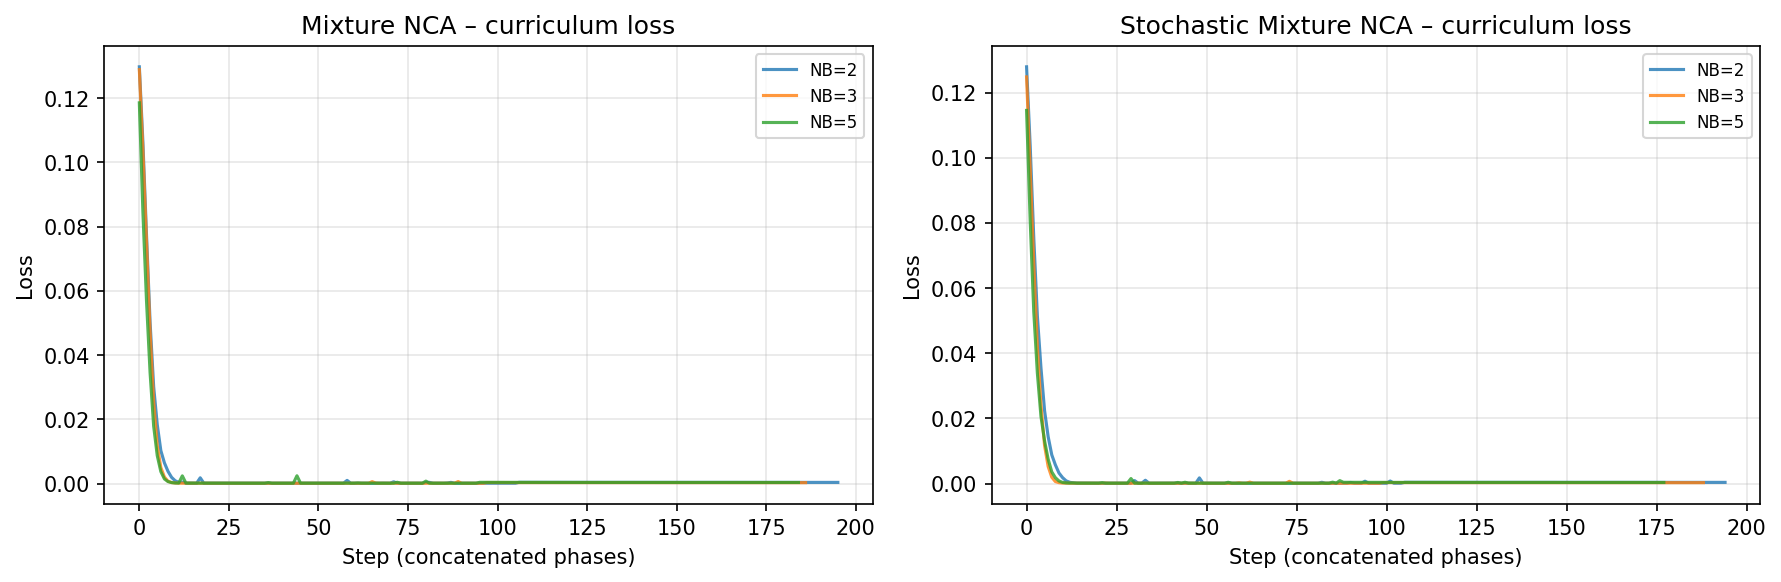
\includegraphics[width=\textwidth]{figs/curriculum/curriculum_loss_curves.png}
  \caption{Curriculum experiment: training loss (linear scale) over curriculum phases. \textbf{Legend:} left panel = Mixture NCA, right = Stochastic Mixture NCA; abscissa = training step; ordinate = loss; one curve per \(NB\in\{2,3,5\}\).}
  \label{fig:impl:curriculum:loss}
\end{figure}

\begin{figure}[H]
  \centering
  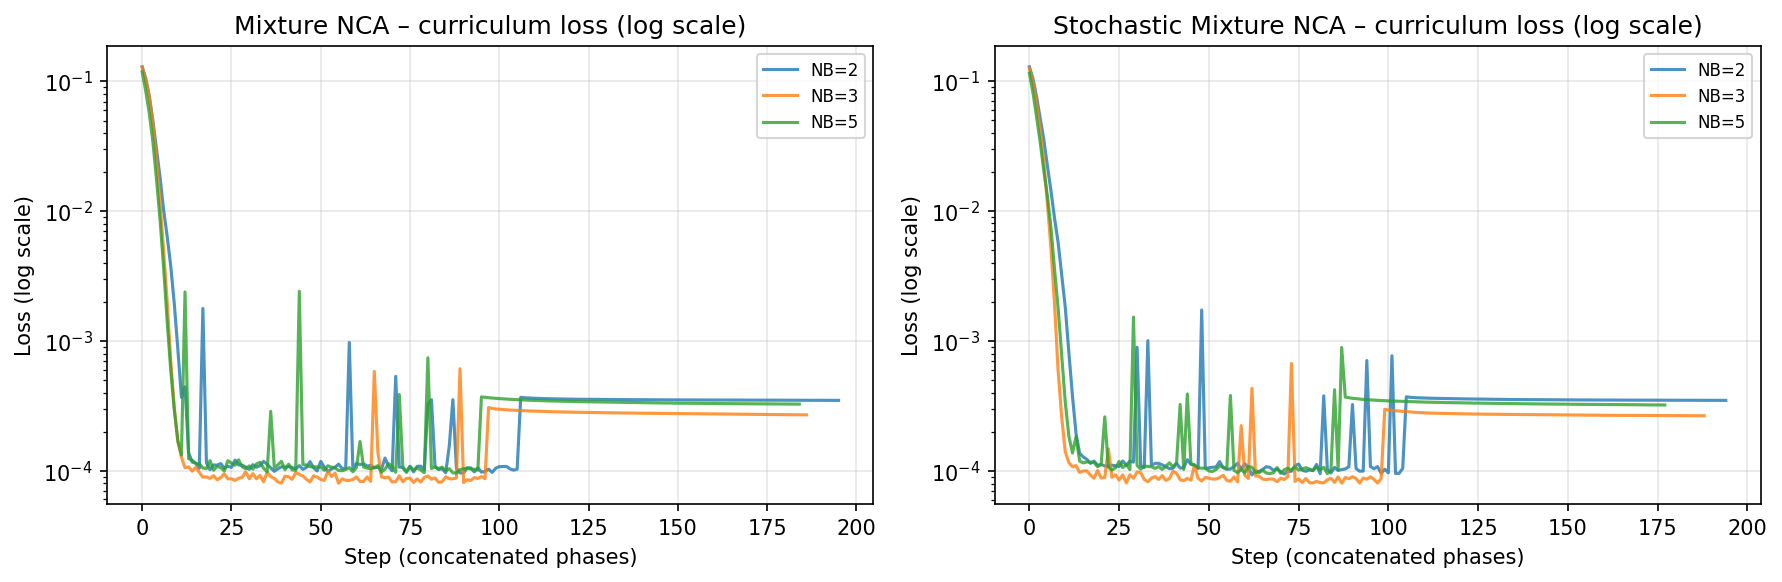
\includegraphics[width=\textwidth]{figs/curriculum/curriculum_loss_curves_log.png}
  \caption{Curriculum experiment: same as Figure~\ref{fig:impl:curriculum:loss} with log-scale ordinate. \textbf{Legend:} same layout (left = Mixture, right = Stochastic; curves = \(NB=2,3,5\)).}
  \label{fig:impl:curriculum:loss_log}
\end{figure}

\subsubsection{Why generated images differ from ground truth}
\label{sec:results:curriculum:limitations}

When we look at the qualitative figures (Figures~\ref{fig:impl:curriculum:ex_nb2} to \ref{fig:impl:curriculum:ex_nb5}), we see that the stochastic variant stays close to the ground truth for \(NB=3\) and \(NB=5\) at all time points, with controlled growth and organic shapes; at \(NB=2\) it still keeps the right scale but the internal structure can look noisier.
The deterministic Mixture NCA, on the other hand, matches the ground truth only early on (around \(t=10\)). As time goes on it starts to diverge: the pattern expands in an uncontrolled way, becomes blocky and homogeneous, and by \(t=500\) the generated tissue often has a different layout, a different mix of cell types, and a tendency to fill the grid instead of evolving like the simulator.

Several factors contribute.
During training we use teacher forcing: at every step we feed the model the true state from the dataset, so small errors do not accumulate and the loss can stay low.
At evaluation we do the opposite: we run free rollouts, where the model only sees its own previous output. In that regime, a small mistake at step 10 is fed into step 11, and the error can grow over time. By step 500 the trajectory may have drifted far from the ground truth even if the model had learned the short-term dynamics well.
A second point is what we actually optimise: the loss is a step-by-step mean squared error over the training window, which encourages correct one-step predictions but does not directly reward how well a long unrolled trajectory matches a single ground-truth run.
For the stochastic model there is an extra nuance: at each step we sample a rule, so different random seeds produce different trajectories; the ground truth we compare against is just one possible realisation of the simulator, and part of the ``difference'' we see is therefore normal variability between runs, not only a failure of the model.
Finally, the last curriculum phase uses 500-step windows but with fewer epochs and a smaller learning rate, so we may stop before the model has fully learned to stay on track for the full 500 steps.

Several directions could be explored to reduce the gap at long times (see also \cref{sec:conc:future}): training longer on 500-step windows or adding more curriculum phases; computing a validation loss with free rollouts and using it for early stopping; adding losses that target the final state of a rollout; or using scheduled teacher forcing so that during training the model gradually sees the true state less often.
At evaluation, running multiple rollouts and averaging or selecting among them could improve the metrics.
The current experiment already shows that the neighbourhood-size effect carries over to the long-horizon curriculum setting and that a larger \(NB\) helps at 100 and 500 steps, especially for the stochastic model.

%-------------------------------------------------------------------
\section{Why evaluation protocol matters}
\label{sec:results:evaluation}
%-------------------------------------------------------------------

A methodological result of this thesis is that \textbf{the evaluation protocol matters}: it can determine whether neighbourhood effects are visible at all. Neighbourhood comparisons are most interpretable when:
\begin{enumerate}
\item training and evaluation are aligned in terms of rule-selection behaviour (e.g., consistent sampling/temperature decisions), and
\item models are evaluated at \textbf{multiple rollout horizons}, because some neighbourhood differences only emerge as errors accumulate over time.
\end{enumerate}

This point is central to the thesis takeaway: if the model already fails because of train--test mismatch (e.g.\ heavy reliance on teacher forcing during training but free rollout at evaluation), neighbourhood effects can be \textbf{masked} by broader instability.

%-------------------------------------------------------------------
\section{Segmentation on BBBC031 (synthetic benchmark)}
\label{sec:results:bbbc031}
%-------------------------------------------------------------------

To complement the synthetic tissue experiments, the thesis also evaluates the extended Stochastic Mixture NCA on the synthetic cell-imaging benchmark BBBC031 (\cref{sec:impl:bbbc031}), where the model must ``grow'' a segmentation mask from seed points (cell centroids) toward a fixed ground-truth target.
In that experiment each model is trained on one image and evaluated on the same image (in-sample); generalization to held-out images is not assessed.

\subsection{Loss curves and optimisation stability}

Training with the default learning rate (\(10^{-3}\)) and 4000 steps yields a clear asymmetry: \(NB=3\) converges to low loss on all five images, while \(NB=7\) either diverges (two images) or settles at much higher loss (three images).
We therefore consider additional training schedules for \(NB=7\) (described in \cref{sec:impl:bbbc031:schedules}); unless stated otherwise, the \(NB=7\) results reported below refer to the re-trained run (lower learning rate, 6000 steps).

\begin{figure}[H]
  \centering
  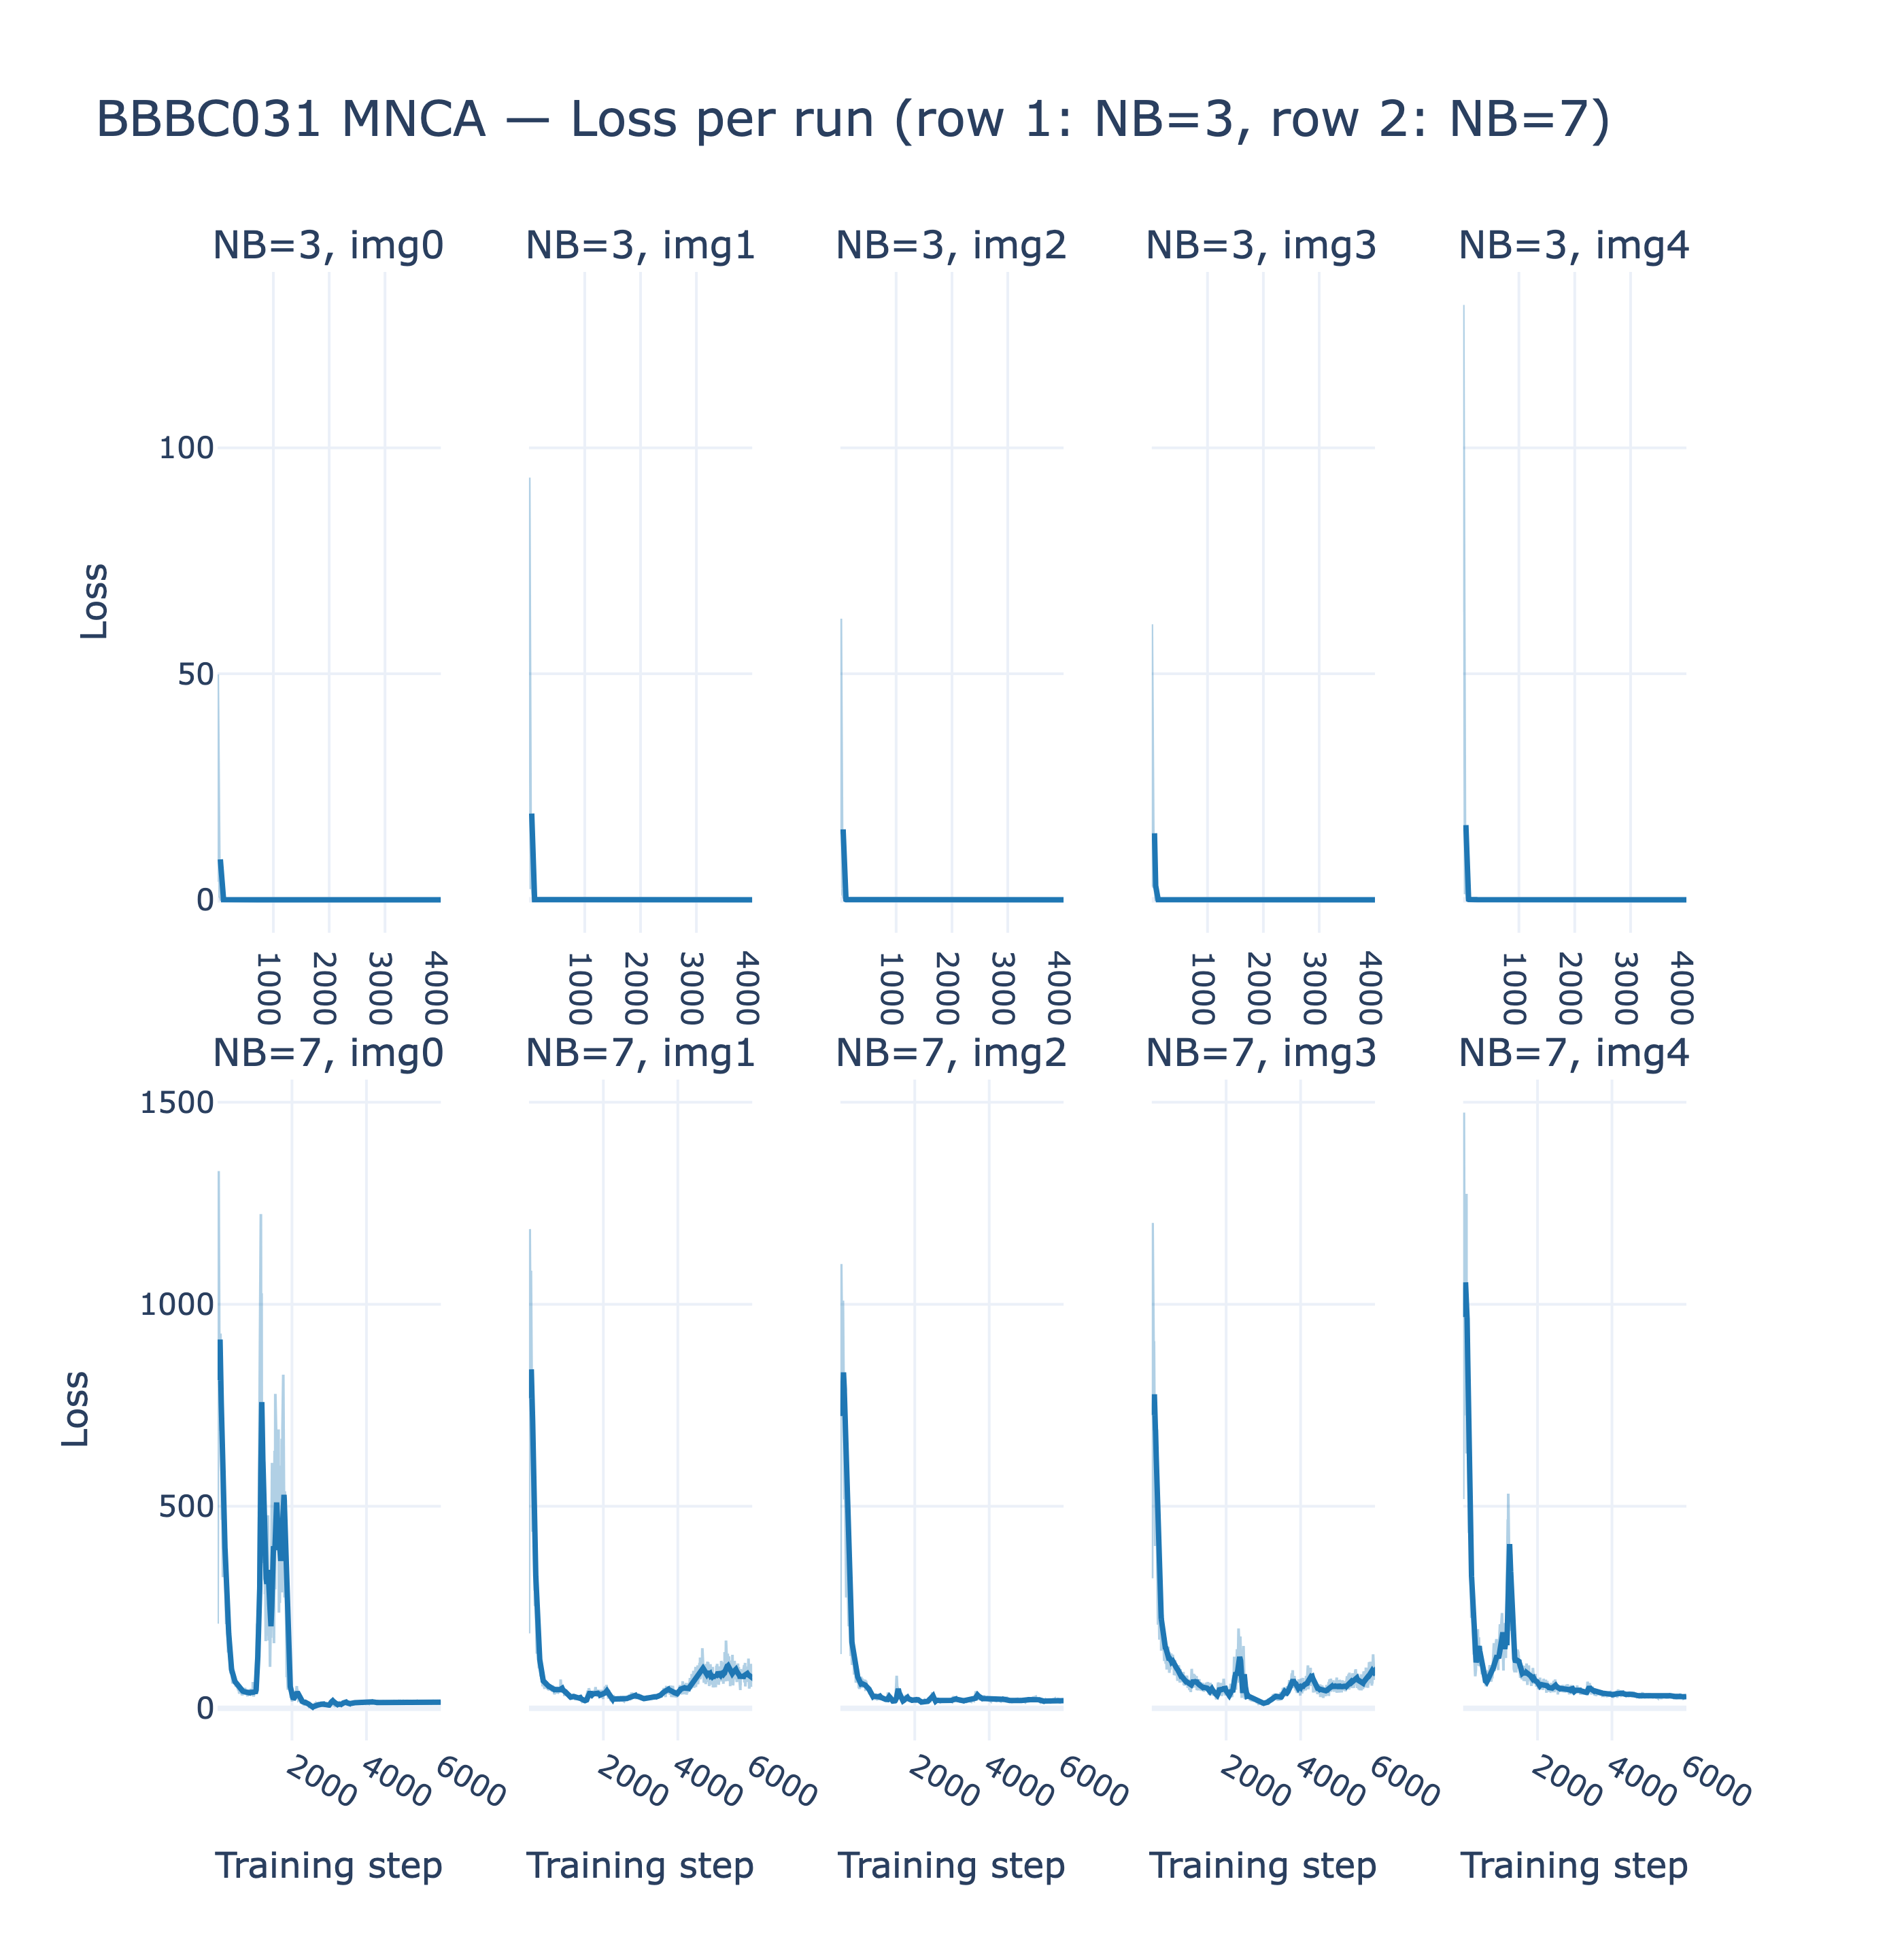
\includegraphics[width=\textwidth]{figs/bbbc031/bbbc031_loss_curves.png}
  \caption{BBBC031: training loss per run. \textbf{Legend:} top row = \(NB=3\) (five images img0--img4, 4000 steps); bottom row = \(NB=7\) re-trained (five images, 6000 steps); abscissa = training step; ordinate = loss; one subplot per image.}
  \label{fig:impl:bbbc031:loss_curves}
\end{figure}

\begin{figure}[H]
  \centering
  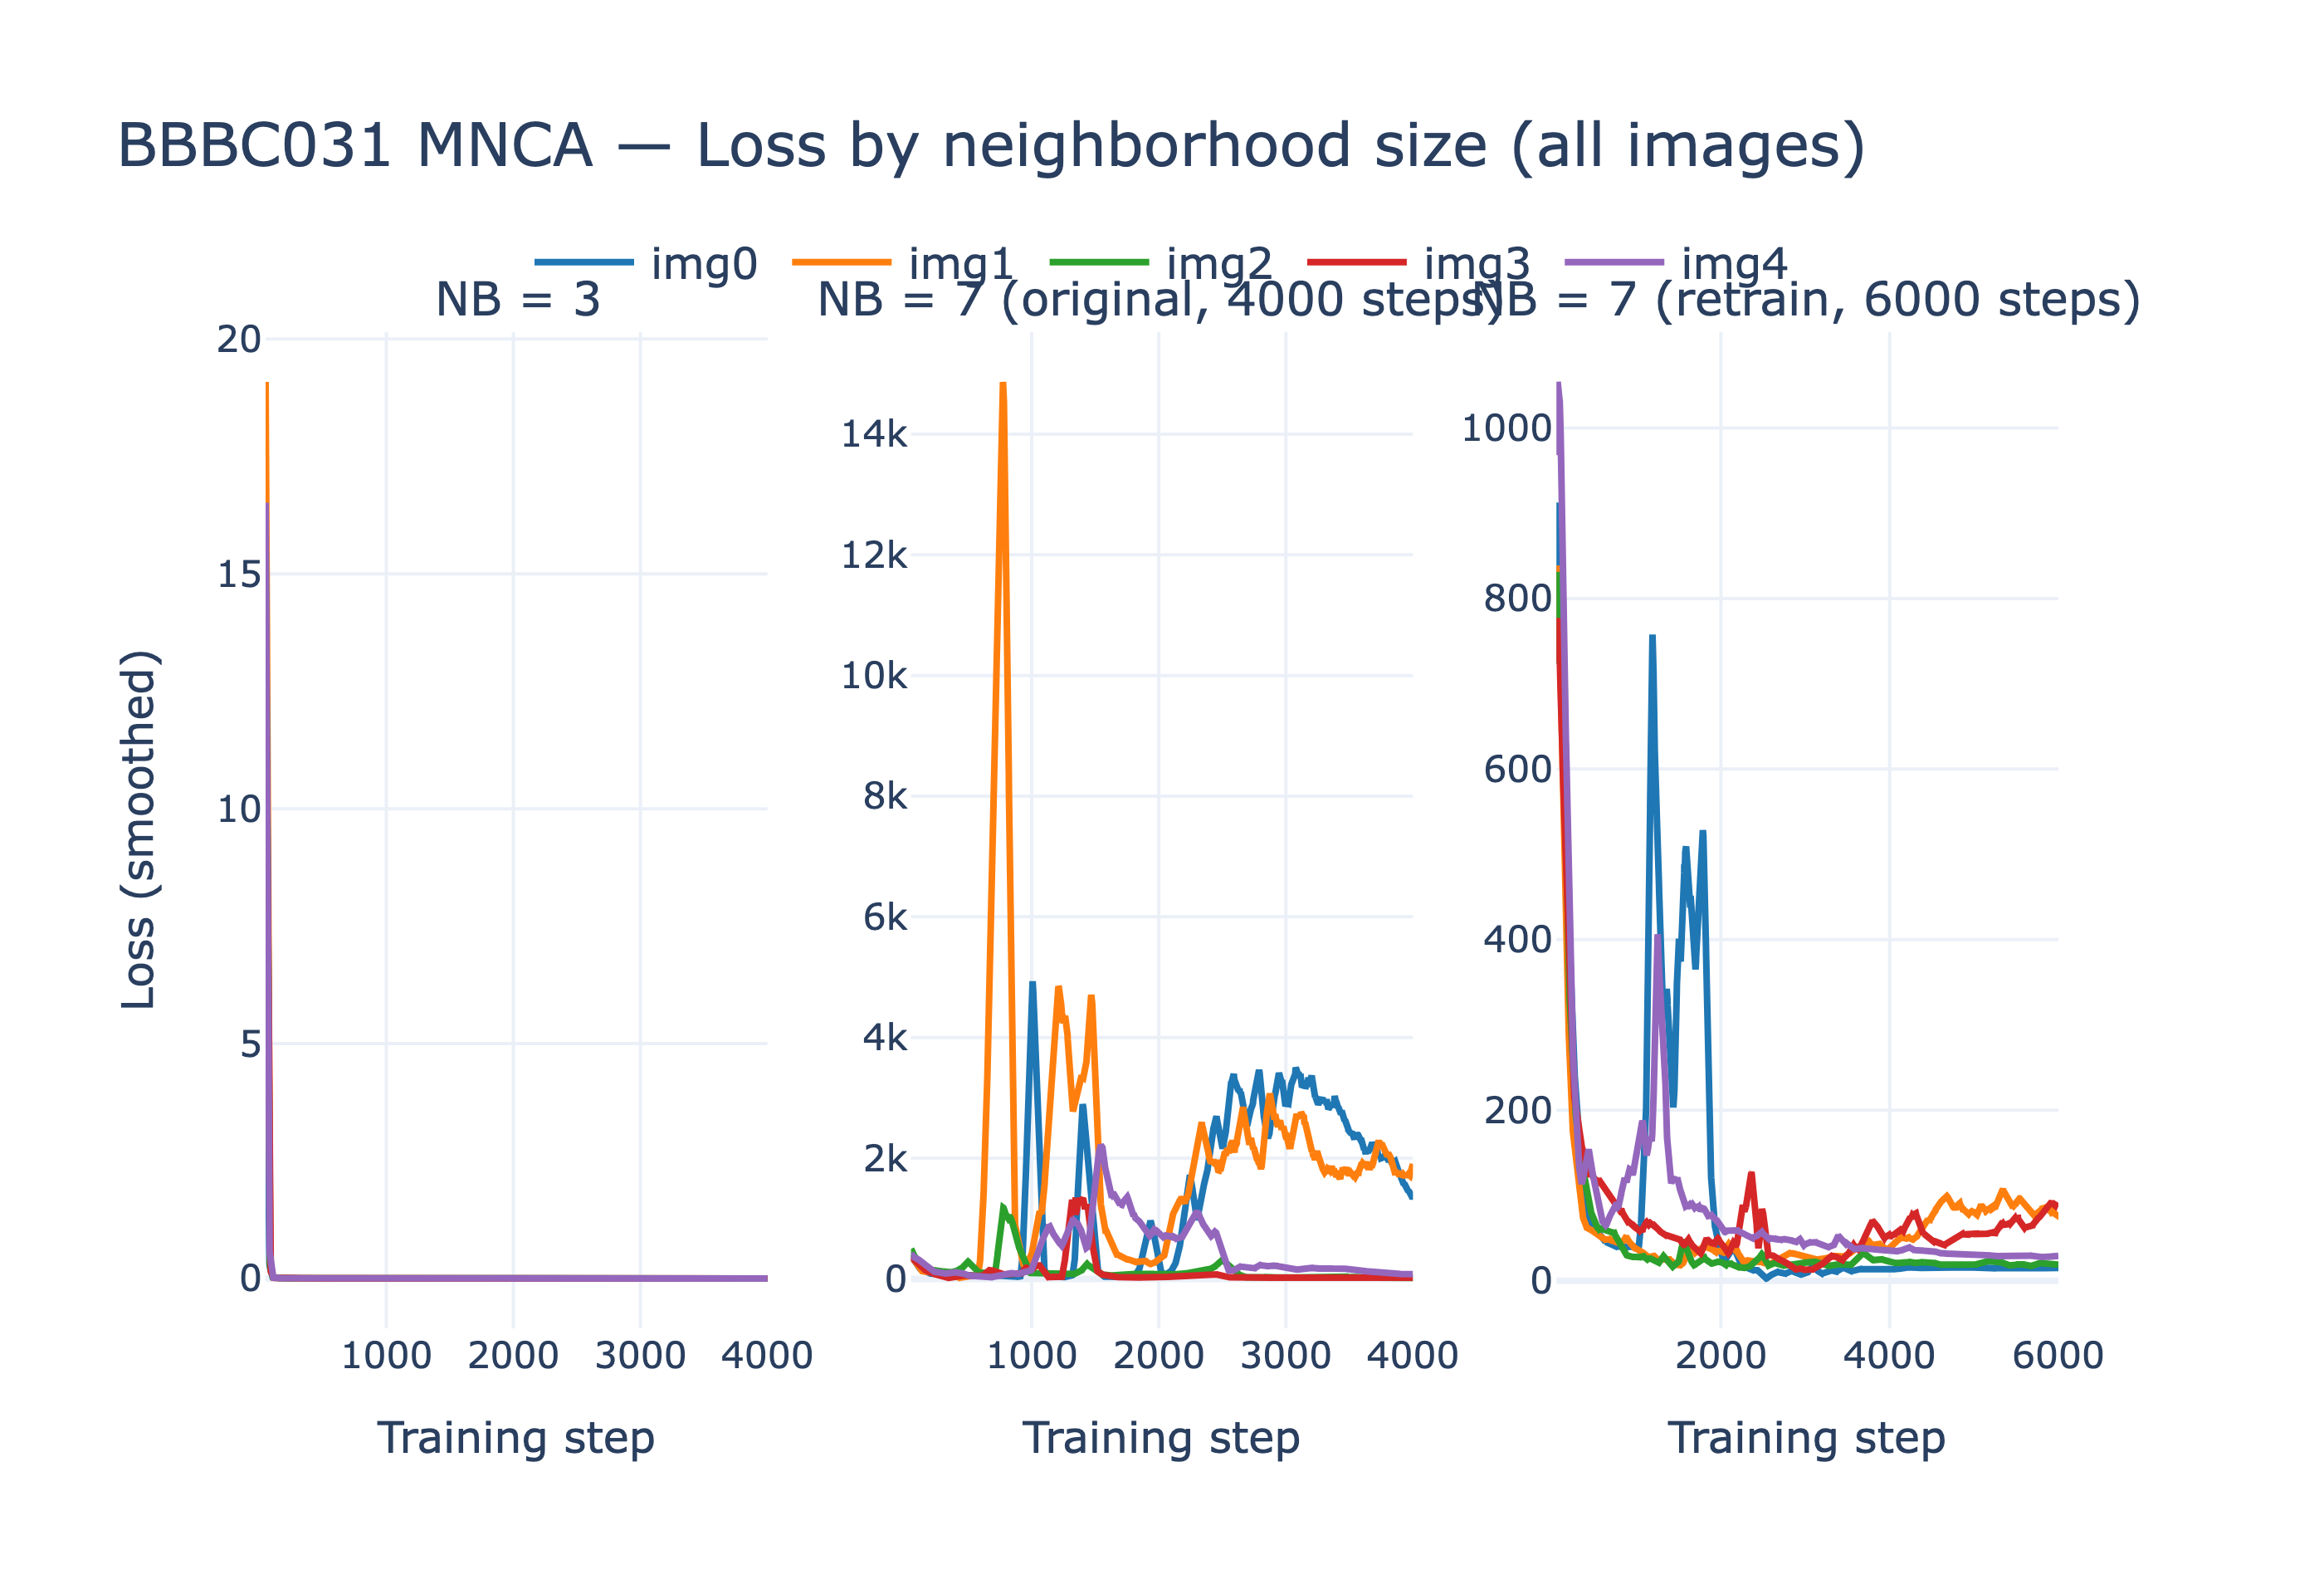
\includegraphics[width=\textwidth]{figs/bbbc031/bbbc031_loss_by_NB.png}
  \caption{BBBC031: loss by neighbourhood size (smoothed). \textbf{Legend:} three panels = \(NB=3\), \(NB=7\) original (4000 steps), \(NB=7\) re-trained (6000 steps); abscissa = training step; ordinate = loss; one curve per image (img0--img4).}
  \label{fig:impl:bbbc031:loss_by_nb}
\end{figure}

\begin{figure}[H]
  \centering
  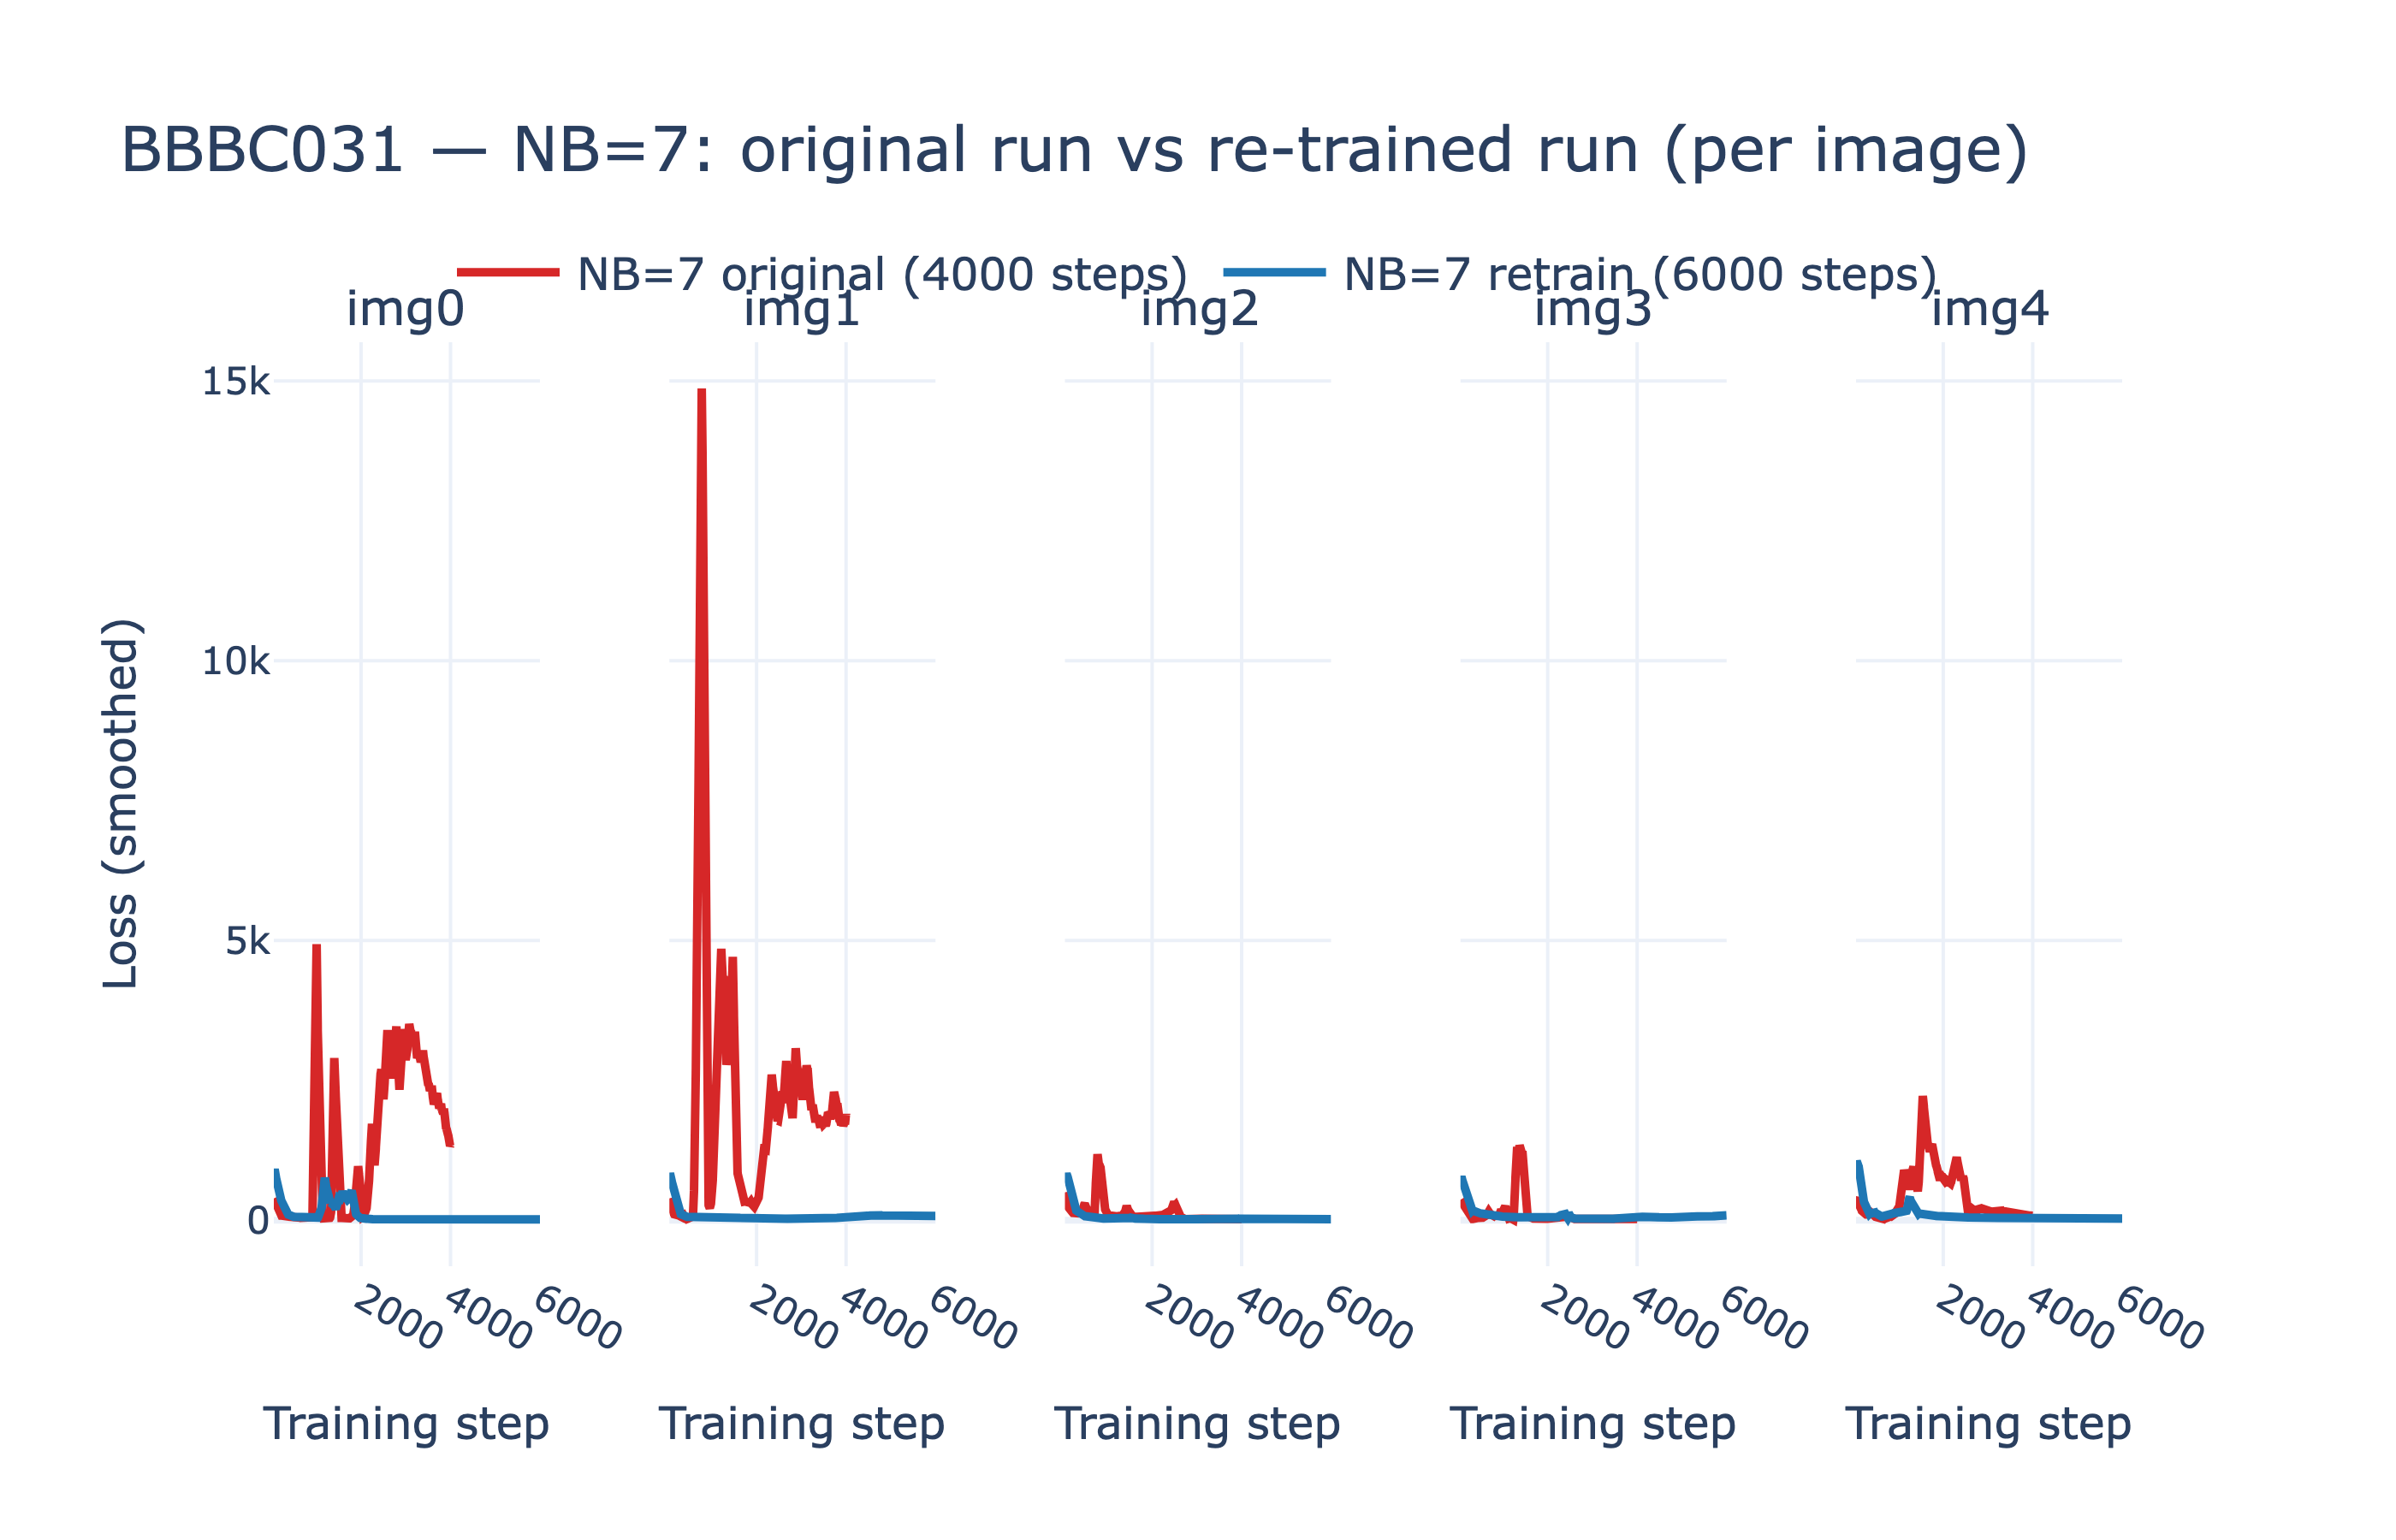
\includegraphics[width=\textwidth]{figs/bbbc031/bbbc031_NB7_original_vs_retrain.png}
  \caption{BBBC031: \(NB=7\) original vs.\ re-trained loss. \textbf{Legend:} one panel per image (img0--img4); abscissa = training step; ordinate = smoothed loss; two curves per panel = original run (4000 steps) and re-trained run (6000 steps).}
  \label{fig:impl:bbbc031:nb7_compare}
\end{figure}

\subsection{Segmentation metrics}

% BBBC031 MNCA metrics table (auto-generated by bbbc031_metrics_thesis.py)
% IoU, Dice, MSE on Stochastic checkpoints NB=3 and NB=7, 20 simulation steps.
% Requires \usepackage{booktabs} in the preamble.
\begin{table}[ht]
\centering
\caption{BBBC031 segmentation metrics: IoU, Dice and MSE (RGBA) per image and neighborhood size (NB).}
\label{tab:bbbc031_metrics}
\begin{tabular}{l|ccc|ccc}
\toprule
Image & \multicolumn{3}{c}{NB=3} & \multicolumn{3}{c}{NB=7} \\
(idx) & IoU & Dice & MSE & IoU & Dice & MSE \\
\midrule
0 & 1.000 & 1.000 & 2.9119e-04 & 0.077 & 0.144 & 3.2822e-01 \\
1 & 0.997 & 0.998 & 1.1005e-03 & 0.171 & 0.292 & 2.9403e-01 \\
2 & 1.000 & 1.000 & 2.8898e-04 & 0.031 & 0.060 & 2.8869e-01 \\
3 & 1.000 & 1.000 & 1.4917e-04 & 0.366 & 0.536 & 3.3028e-01 \\
4 & 0.991 & 0.996 & 2.2697e-03 & 0.056 & 0.107 & 3.0516e-01 \\
\bottomrule
\end{tabular}
\end{table}


\subsubsection{NB=7 original vs.\ re-trained}
\label{sec:impl:bbbc031:retrain}
\vspace{-0.5em}
Re-training \(NB=7\) with a lower learning rate (\(3\times10^{-4}\)) and a longer run (6000 steps) avoids divergence and improves segmentation overlap metrics, although performance remains below the \(NB=3\) reference under the schedules explored.
\vspace{-1.5em}
\paragraph{Comparison of segmentation outputs: \(NB=7\) original vs.\ re-trained.}
Figure~\ref{fig:impl:bbbc031:nb7_output_compare} compares the segmentation outputs (after 20 simulation steps) of the original \(NB=7\) model with the re-trained one, for all five images.
Each row shows, from left to right: ground truth, prediction of the original run (4000 steps, default learning rate), and prediction of the re-trained run (6000 steps, lower learning rate).
\vspace{-0.8em}
\begin{figure}[H]
  \centering
  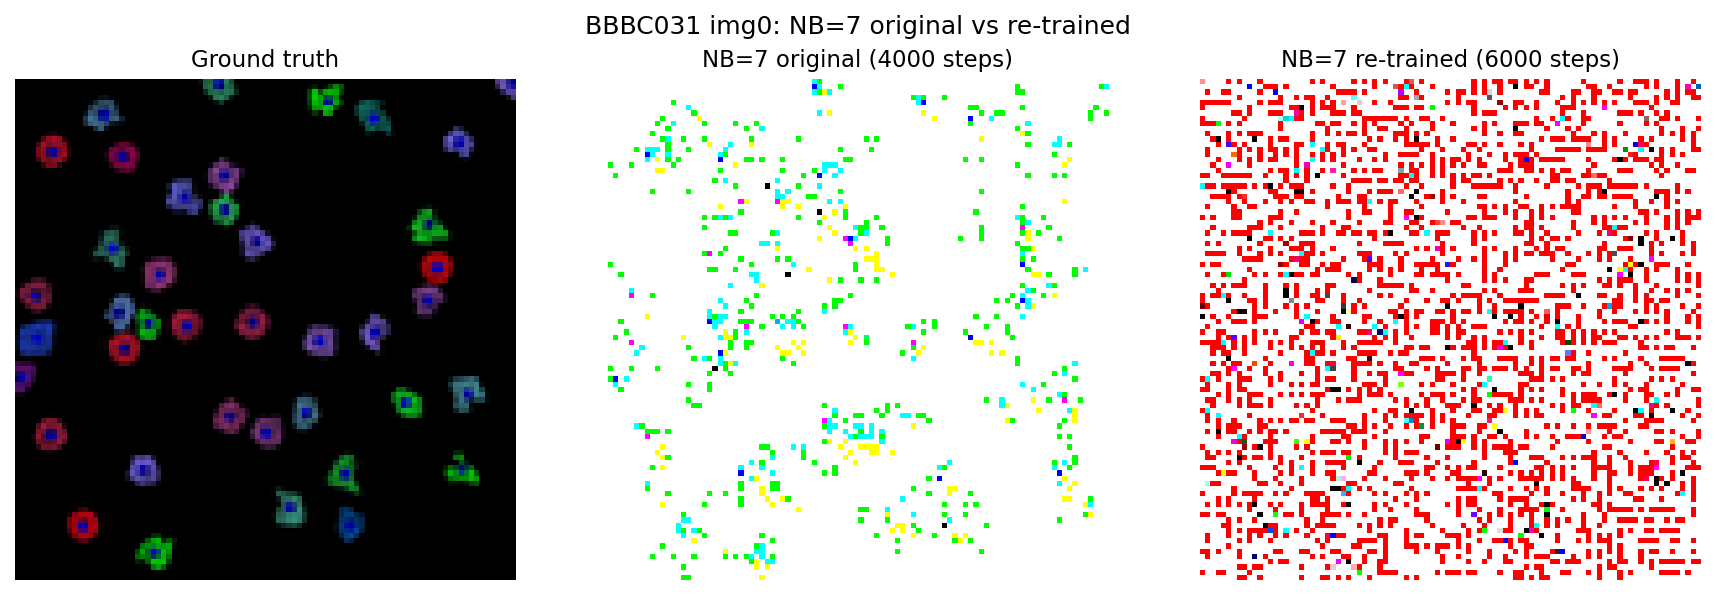
\includegraphics[width=0.98\textwidth]{figs/bbbc031/bbbc031_NB7_original_vs_retrain_img0.png}\\[0.25em]
  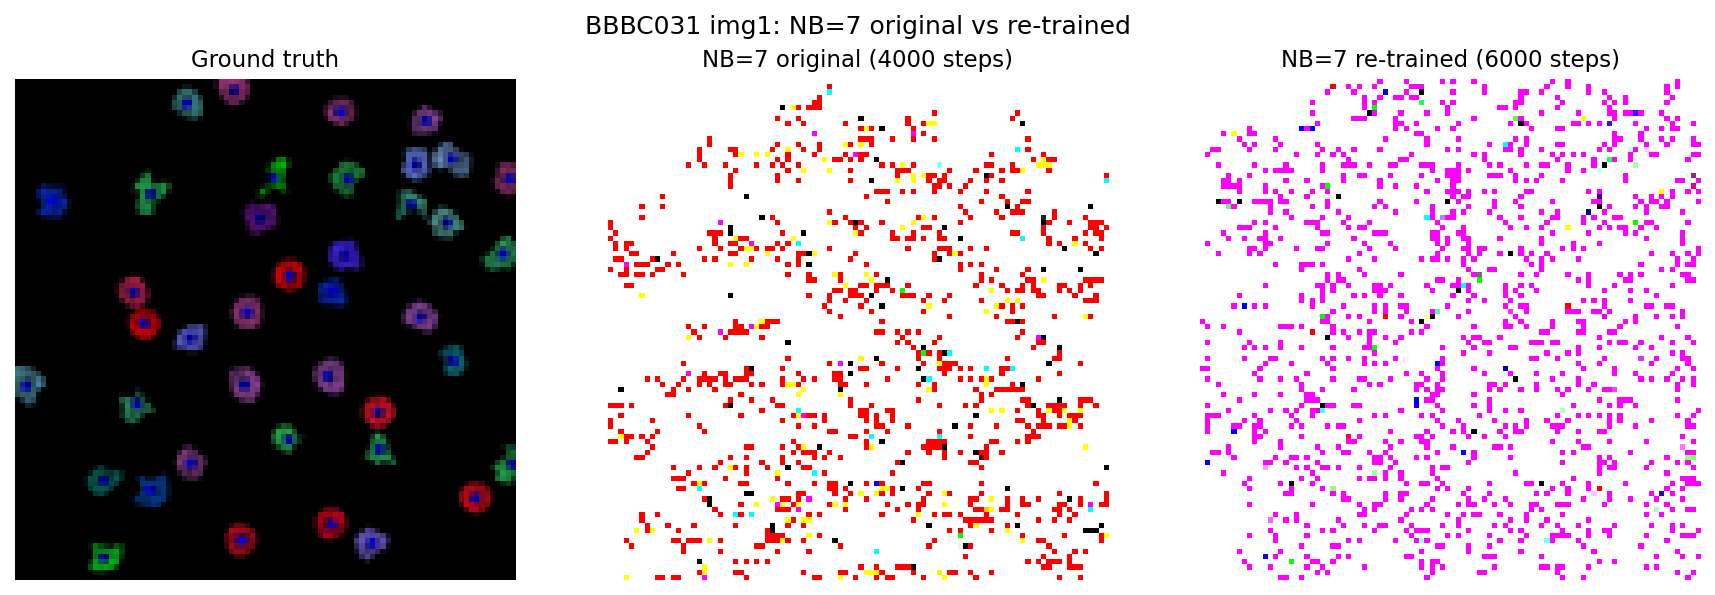
\includegraphics[width=0.98\textwidth]{figs/bbbc031/bbbc031_NB7_original_vs_retrain_img1.png}\\[0.25em]
  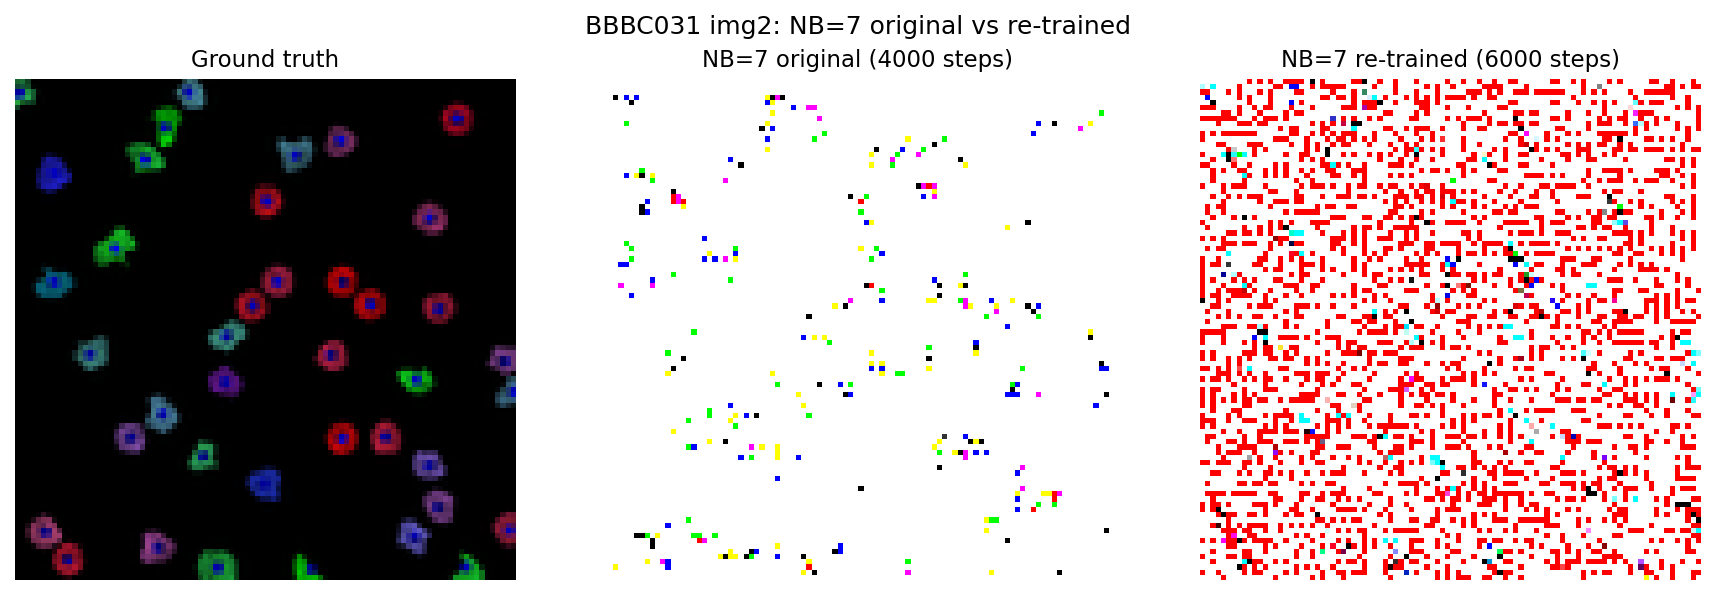
\includegraphics[width=0.98\textwidth]{figs/bbbc031/bbbc031_NB7_original_vs_retrain_img2.png}\\[0.25em]
  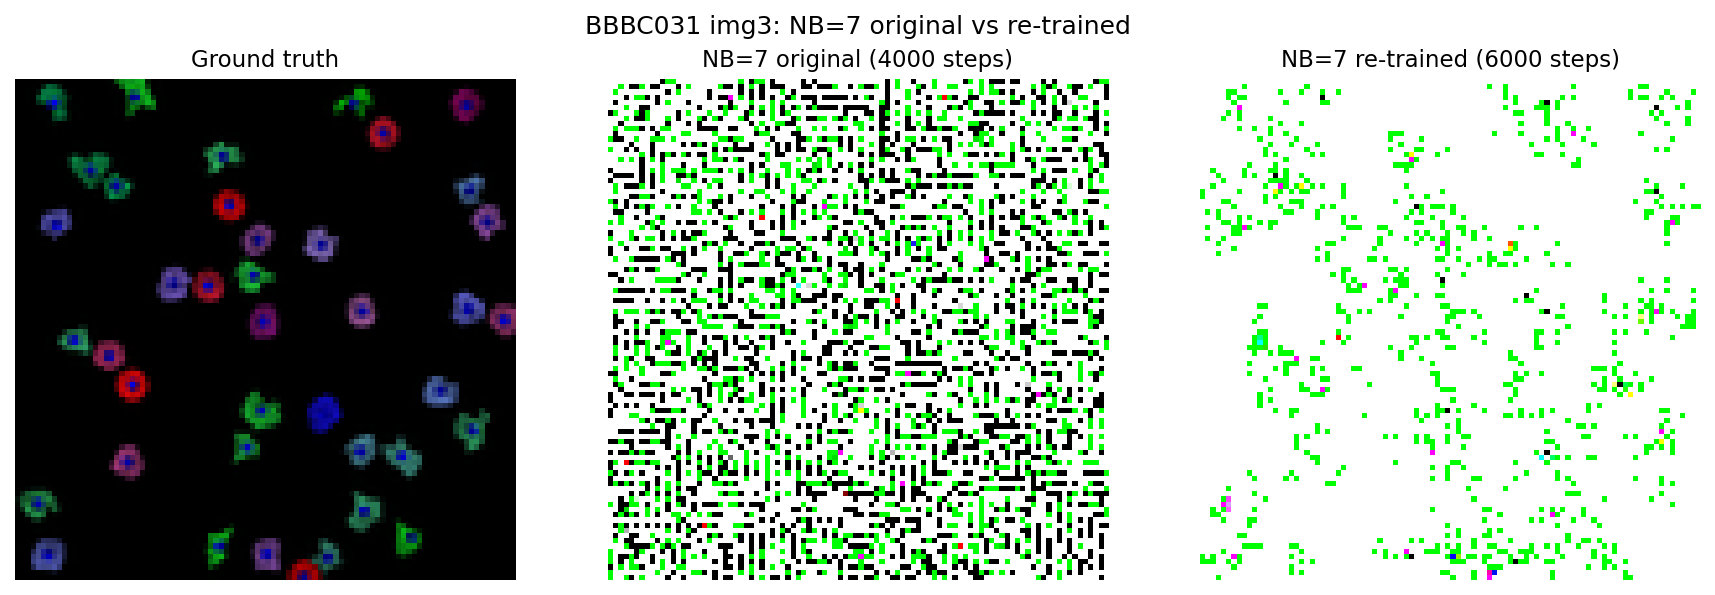
\includegraphics[width=0.98\textwidth]{figs/bbbc031/bbbc031_NB7_original_vs_retrain_img3.png}\\[0.25em]
  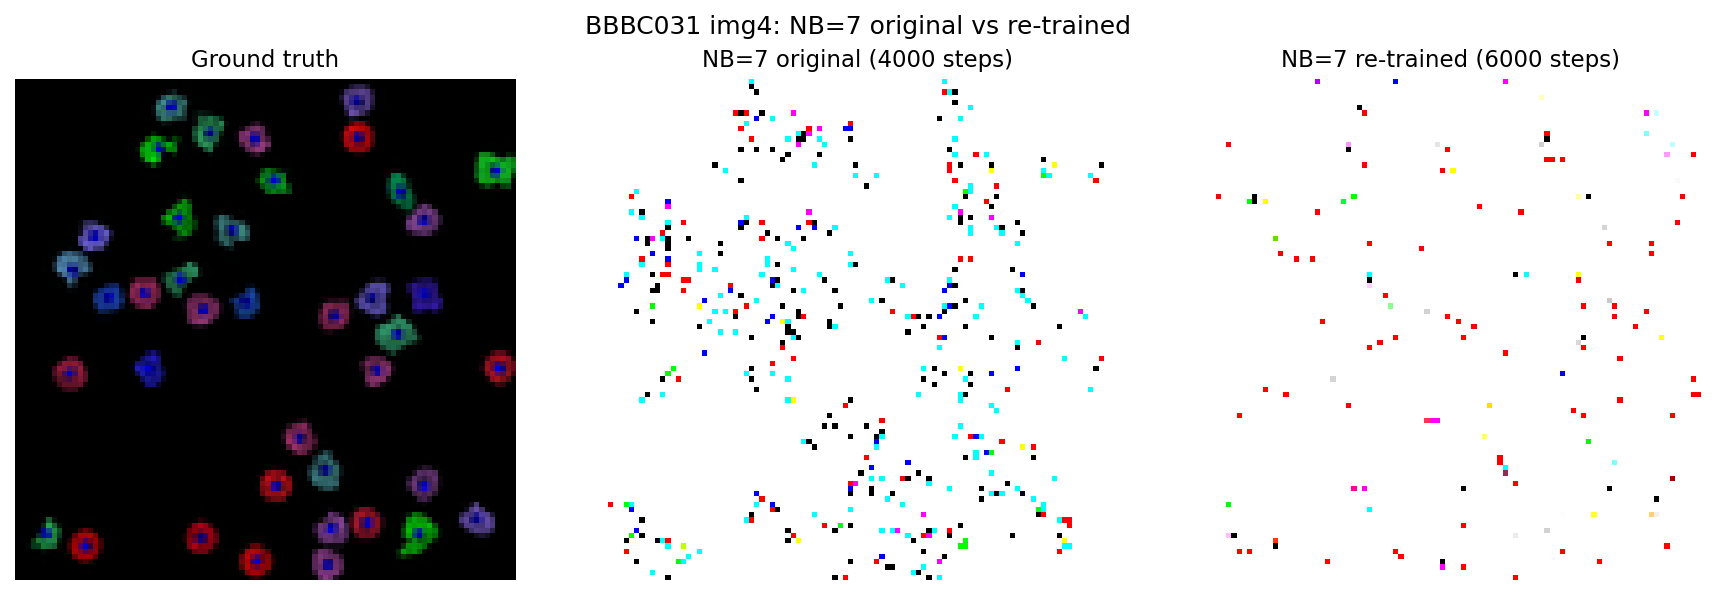
\includegraphics[width=0.98\textwidth]{figs/bbbc031/bbbc031_NB7_original_vs_retrain_img4.png}
  \vspace{0.5em}
  \caption{BBBC031: segmentation outputs for \(NB=7\) after 20 simulation steps. \textbf{Legend:} each row = one image (img0--img4); columns = ground-truth mask, prediction original run (4000 steps), prediction re-trained run (6000 steps).}
  \label{fig:impl:bbbc031:nb7_output_compare}
\end{figure}

\Cref{tab:bbbc031_NB7_comparison} reports the same comparison in terms of IoU, Dice, and MSE.

% NB=7 original vs re-trained metrics (auto-generated)
% IoU/Dice on alpha mask; MSE on RGBA; MSE_RGB on RGB only (colour fidelity).
% Requires \usepackage{booktabs} in the preamble.
\begin{table}[H]
\centering
\caption{BBBC031: comparison between NB=7 original (4000 steps, LR $10^{-3}$) and re-trained (6000 steps, LR $3\times10^{-4}$). IoU and Dice use the alpha channel; MSE is on all RGBA channels; MSE\_RGB is on RGB only (colour fidelity).}
\label{tab:bbbc031_NB7_comparison}
\vspace{0.5em}
\resizebox{\textwidth}{!}{%
\begin{tabular}{c|cccc|cccc|cccc}
\toprule
Image & \multicolumn{4}{c}{NB=7 original} & \multicolumn{4}{c}{NB=7 re-trained} & \multicolumn{4}{c}{$\Delta$ (retrain $-$ orig)} \\
(idx) & IoU & Dice & MSE & MSE\_RGB & IoU & Dice & MSE & MSE\_RGB & IoU & Dice & MSE & MSE\_RGB \\
\midrule
0 & 0.095 & 0.174 & 3.3991e-01 & 1.5170e-01 & 0.301 & 0.463 & 3.5285e-01 & 2.3784e-01 & +0.206 & +0.289 & +1.2947e-02 & +8.6140e-02 \\
1 & 0.179 & 0.304 & 2.9670e-01 & 1.2212e-01 & 0.372 & 0.543 & 4.0718e-01 & 3.3381e-01 & +0.193 & +0.238 & +1.1048e-01 & +2.1169e-01 \\
2 & 0.030 & 0.058 & 2.8579e-01 & 5.7618e-02 & 0.291 & 0.451 & 3.6456e-01 & 2.4996e-01 & +0.261 & +0.393 & +7.8779e-02 & +1.9235e-01 \\
3 & 0.361 & 0.531 & 3.3476e-01 & 2.3358e-01 & 0.099 & 0.180 & 3.3511e-01 & 1.4645e-01 & -0.263 & -0.351 & +3.5074e-04 & -8.7135e-02 \\
4 & 0.060 & 0.113 & 3.0988e-01 & 9.9813e-02 & 0.408 & 0.580 & 4.3196e-01 & 3.7886e-01 & +0.349 & +0.467 & +1.2208e-01 & +2.7904e-01 \\
\bottomrule
\end{tabular}%
}
\end{table}


\subsubsection{Qualitative examples: seeds, \(NB=3\), and \(NB=7\)}

\begin{figure}[H]
  \centering
  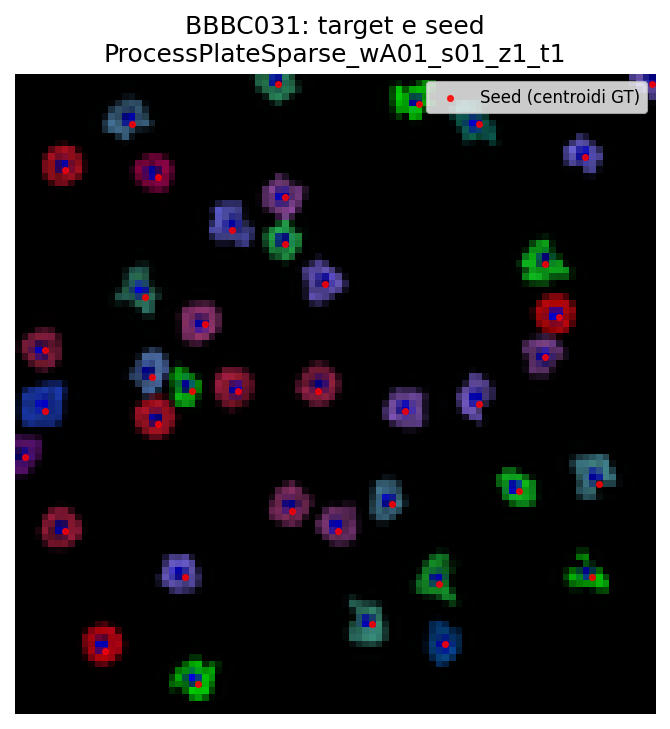
\includegraphics[width=0.7\textwidth]{figs/bbbc031/bbbc031_target_and_seed.png}
  \caption{BBBC031: ground-truth cell mask and seed points. \textbf{Legend:} mask = ground-truth segmentation (CELLMASK); points = cell centroids (seeds); the NCA is initialised from these seeds and run for 20 steps.}
  \label{fig:impl:bbbc031:target_seed}
\end{figure}

\begin{figure}[H]
  \centering
  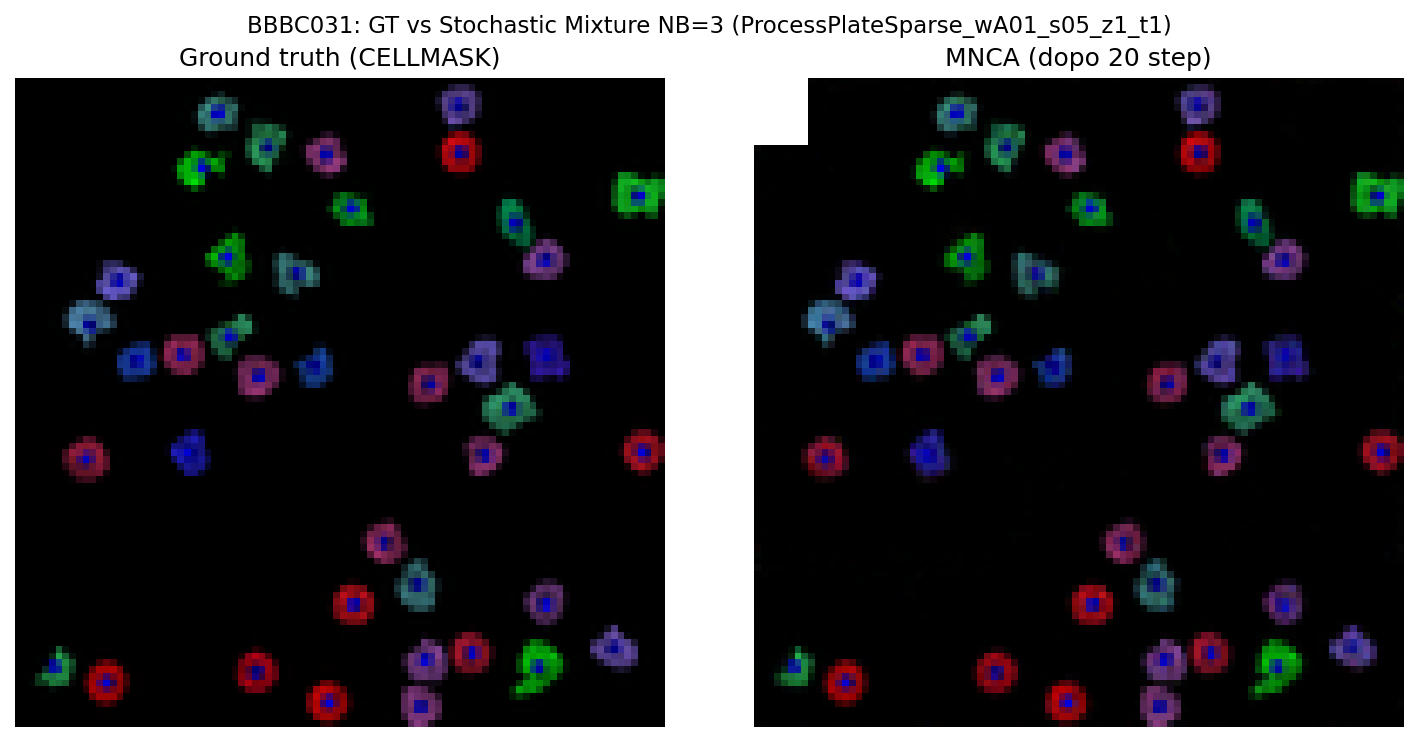
\includegraphics[width=\textwidth]{figs/bbbc031/bbbc031_gt_vs_mnca_trained_here_NB3_stochastic.png}
  \caption{BBBC031: ground truth vs.\ prediction, \(NB=3\). \textbf{Legend:} left = ground-truth mask; right = Stochastic Mixture NCA output after 20 steps.}
  \label{fig:impl:bbbc031:gt_vs_nb3}
\end{figure}

\begin{figure}[H]
  \centering
  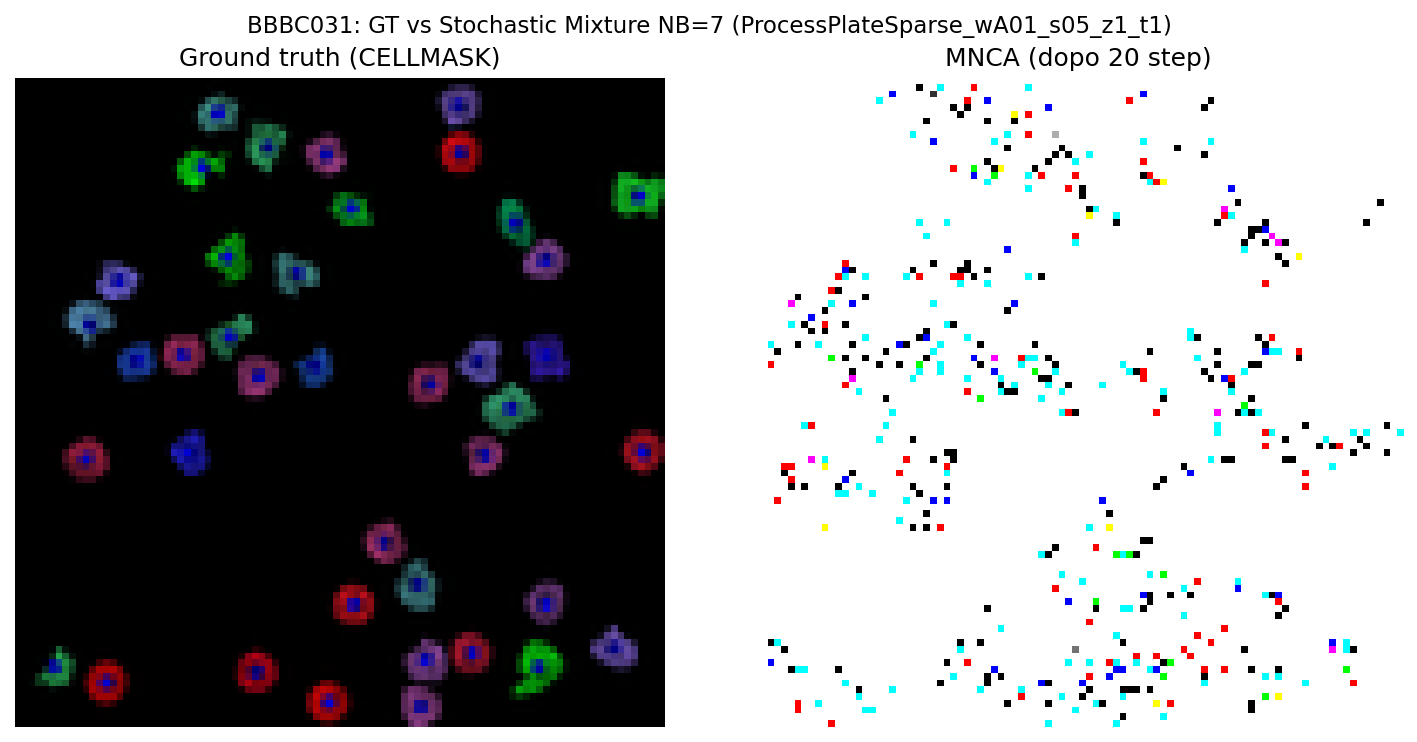
\includegraphics[width=\textwidth]{figs/bbbc031/bbbc031_gt_vs_mnca_trained_here_NB7_stochastic.png}
  \caption{BBBC031: ground truth vs.\ prediction, \(NB=7\) original run. \textbf{Legend:} left = ground-truth mask; right = Stochastic Mixture NCA (\(NB=7\), 4000 steps) after 20 simulation steps.}
  \label{fig:impl:bbbc031:gt_vs_nb7}
\end{figure}

\begin{figure}[H]
  \centering
  \begin{minipage}[t]{0.32\textwidth}
    \centering
    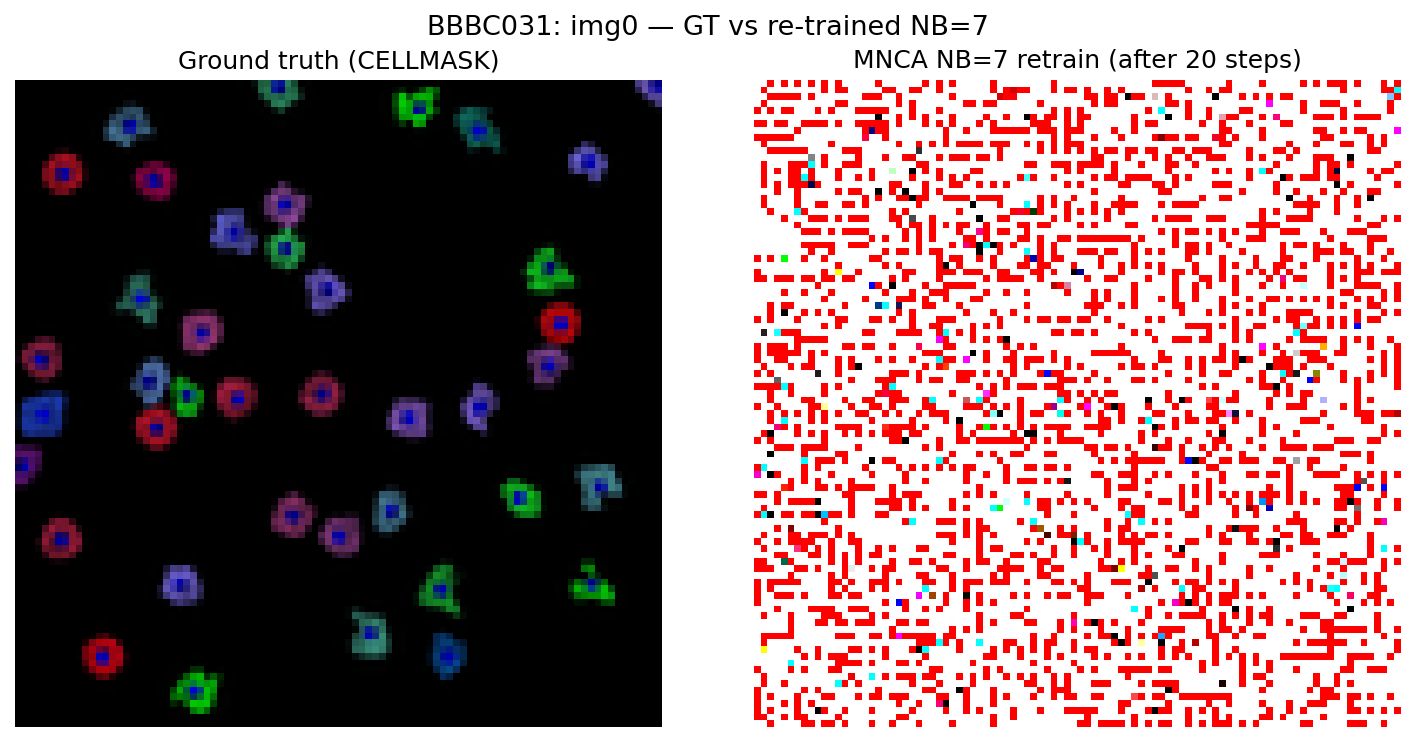
\includegraphics[width=\textwidth]{figs/bbbc031/bbbc031_gt_vs_mnca_NB7_retrain_img0.png}
    \caption*{img0}
  \end{minipage}\hfill
  \begin{minipage}[t]{0.32\textwidth}
    \centering
    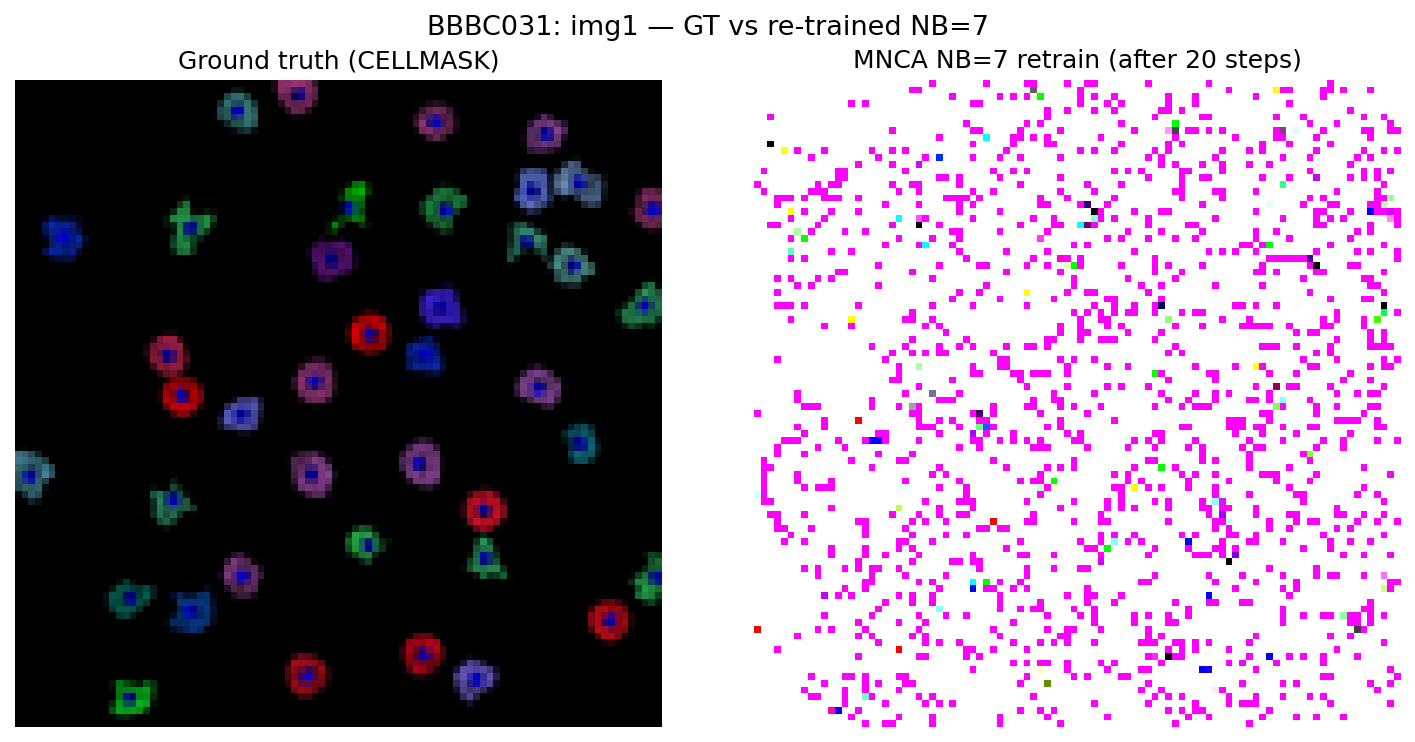
\includegraphics[width=\textwidth]{figs/bbbc031/bbbc031_gt_vs_mnca_NB7_retrain_img1.png}
    \caption*{img1}
  \end{minipage}\hfill
  \begin{minipage}[t]{0.32\textwidth}
    \centering
    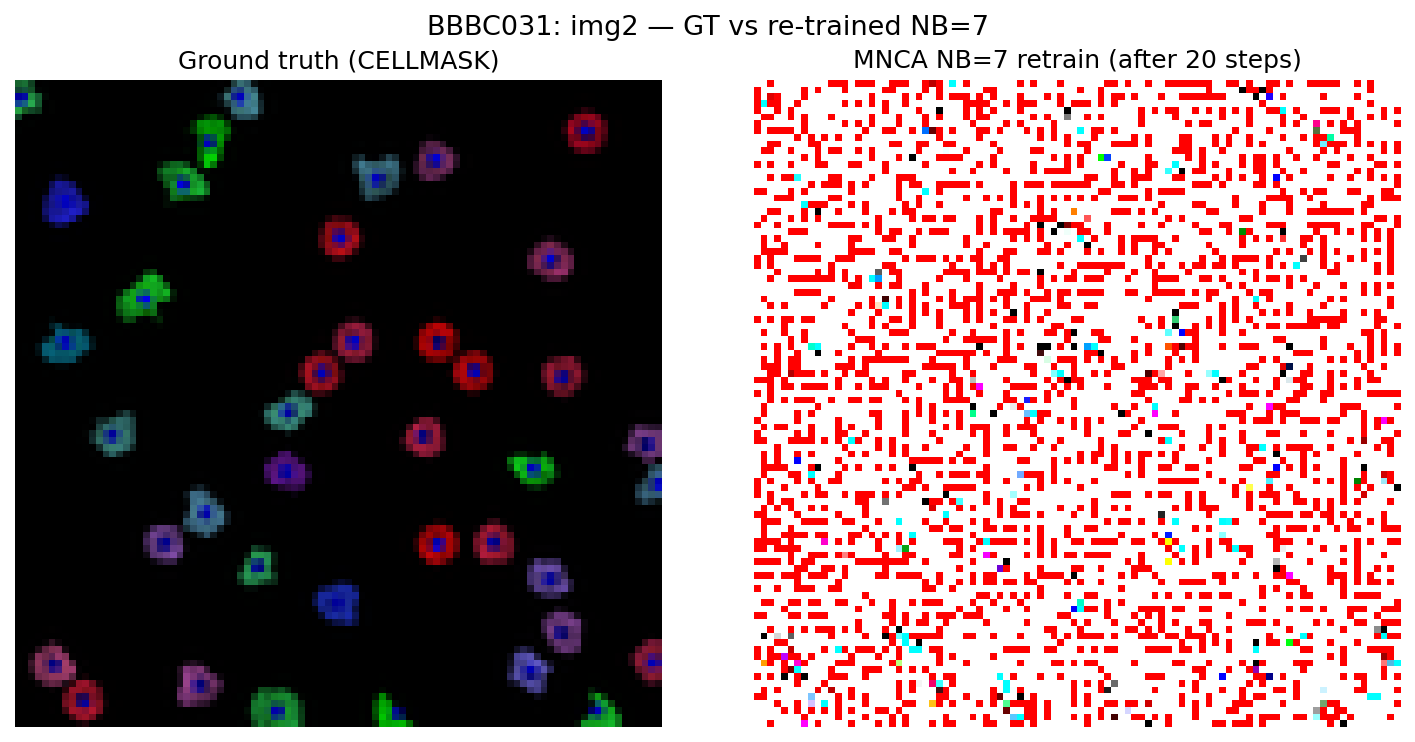
\includegraphics[width=\textwidth]{figs/bbbc031/bbbc031_gt_vs_mnca_NB7_retrain_img2.png}
    \caption*{img2}
  \end{minipage}\\[0.5em]
  \hfill
  \begin{minipage}[t]{0.32\textwidth}
    \centering
    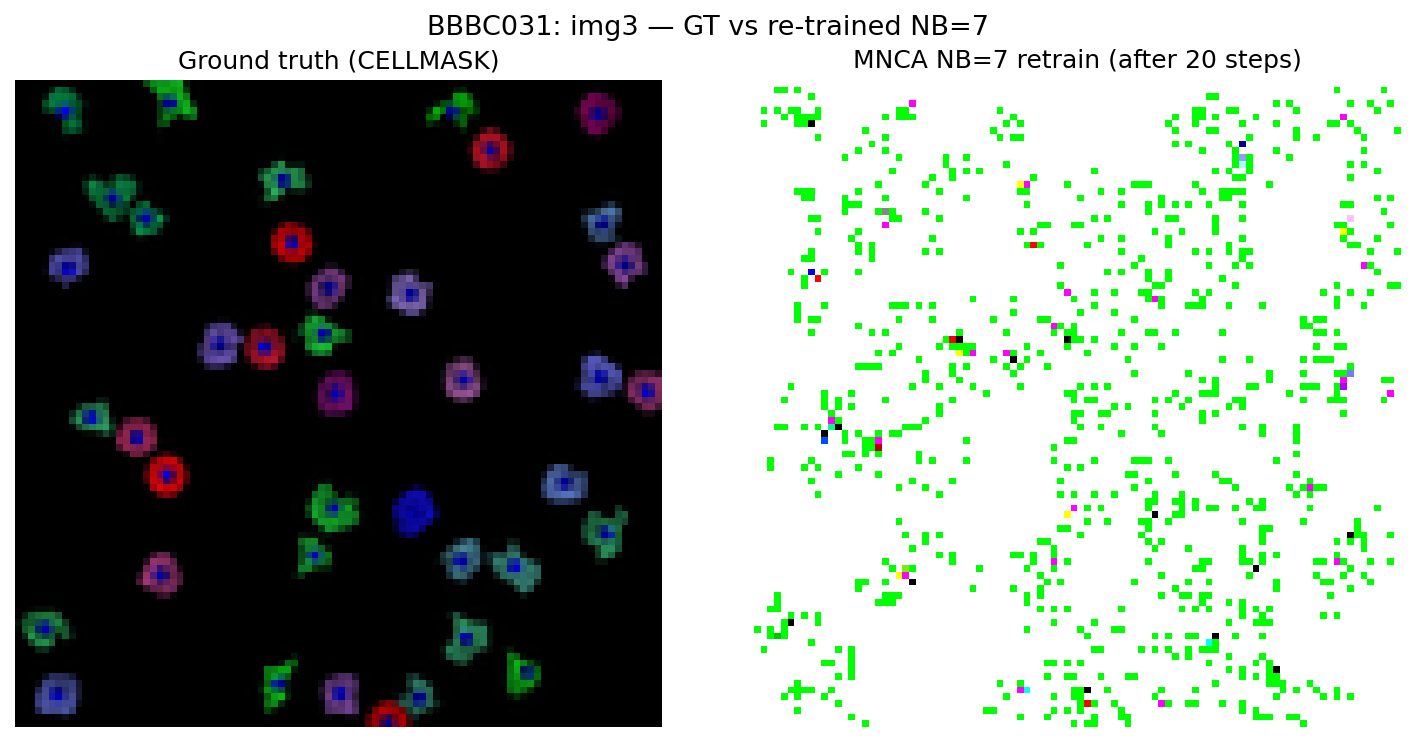
\includegraphics[width=\textwidth]{figs/bbbc031/bbbc031_gt_vs_mnca_NB7_retrain_img3.png}
    \caption*{img3}
  \end{minipage}\hfill
  \begin{minipage}[t]{0.32\textwidth}
    \centering
    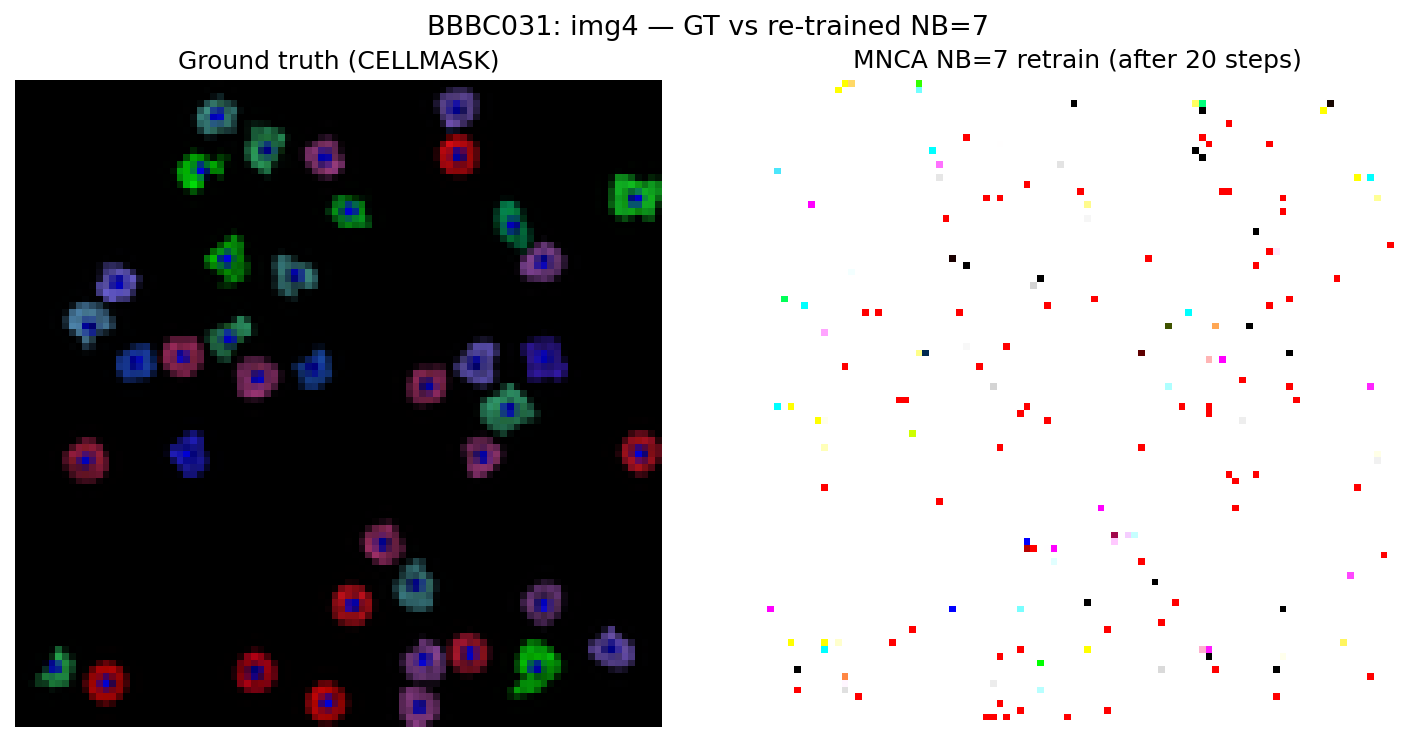
\includegraphics[width=\textwidth]{figs/bbbc031/bbbc031_gt_vs_mnca_NB7_retrain_img4.png}
    \caption*{img4}
  \end{minipage}\hfill
  \caption{BBBC031: outputs from re-trained \(NB=7\) (20 steps). \textbf{Legend:} five panels = img0--img4; each panel = ground truth (left) vs.\ prediction (right).}
  \label{fig:impl:bbbc031:gt_vs_nb7_retrain}
\end{figure}

\subsubsection{Extended re-training at 12\,000 steps}
\label{sec:impl:bbbc031:retrain12k}

To test whether a longer optimisation and a finer learning-rate schedule could reduce the remaining gap for \(NB=7\), we ran an extended re-training at 12\,000 steps (same learning rate as the 6000-step re-training, but with four milestones).

% NB=7 6000 vs 12000 steps metrics (auto-generated)
% Requires \usepackage{booktabs} in the preamble.
\begin{table}[H]
\centering
\caption{BBBC031: segmentation metrics for NB=7 re-trained run at 6000 steps vs extended run at 12000 steps (LR $3\times10^{-4}$, milestones at 4500, 6000, 7500, 9500).}
\label{tab:bbbc031_NB7_6k_vs_12k}
\vspace{0.5em}
\begin{tabular}{c|ccc|ccc|ccc}
\toprule
Image & \multicolumn{3}{c}{6k steps} & \multicolumn{3}{c}{12k steps} & \multicolumn{3}{c}{$\Delta$ (12k $-$ 6k)} \\
(idx) & IoU & Dice & MSE & IoU & Dice & MSE & IoU & Dice & MSE \\
\midrule
0 & 0.299 & 0.460 & 3.5363e-01 & 0.330 & 0.496 & 4.2480e-01 & +0.031 & +0.036 & +7.1169e-02 \\
1 & 0.373 & 0.544 & 4.0621e-01 & 0.420 & 0.592 & 3.3443e-01 & +0.047 & +0.048 & -7.1774e-02 \\
2 & 0.288 & 0.447 & 3.6465e-01 & 0.483 & 0.651 & 4.4987e-01 & +0.195 & +0.204 & +8.5217e-02 \\
3 & 0.089 & 0.163 & 3.2662e-01 & 0.424 & 0.595 & 4.3512e-01 & +0.335 & +0.432 & +1.0850e-01 \\
4 & 0.405 & 0.576 & 4.3086e-01 & 0.991 & 0.996 & 2.4332e-01 & +0.586 & +0.419 & -1.8754e-01 \\
\bottomrule
\end{tabular}
\end{table}


\begin{figure}[H]
  \centering
  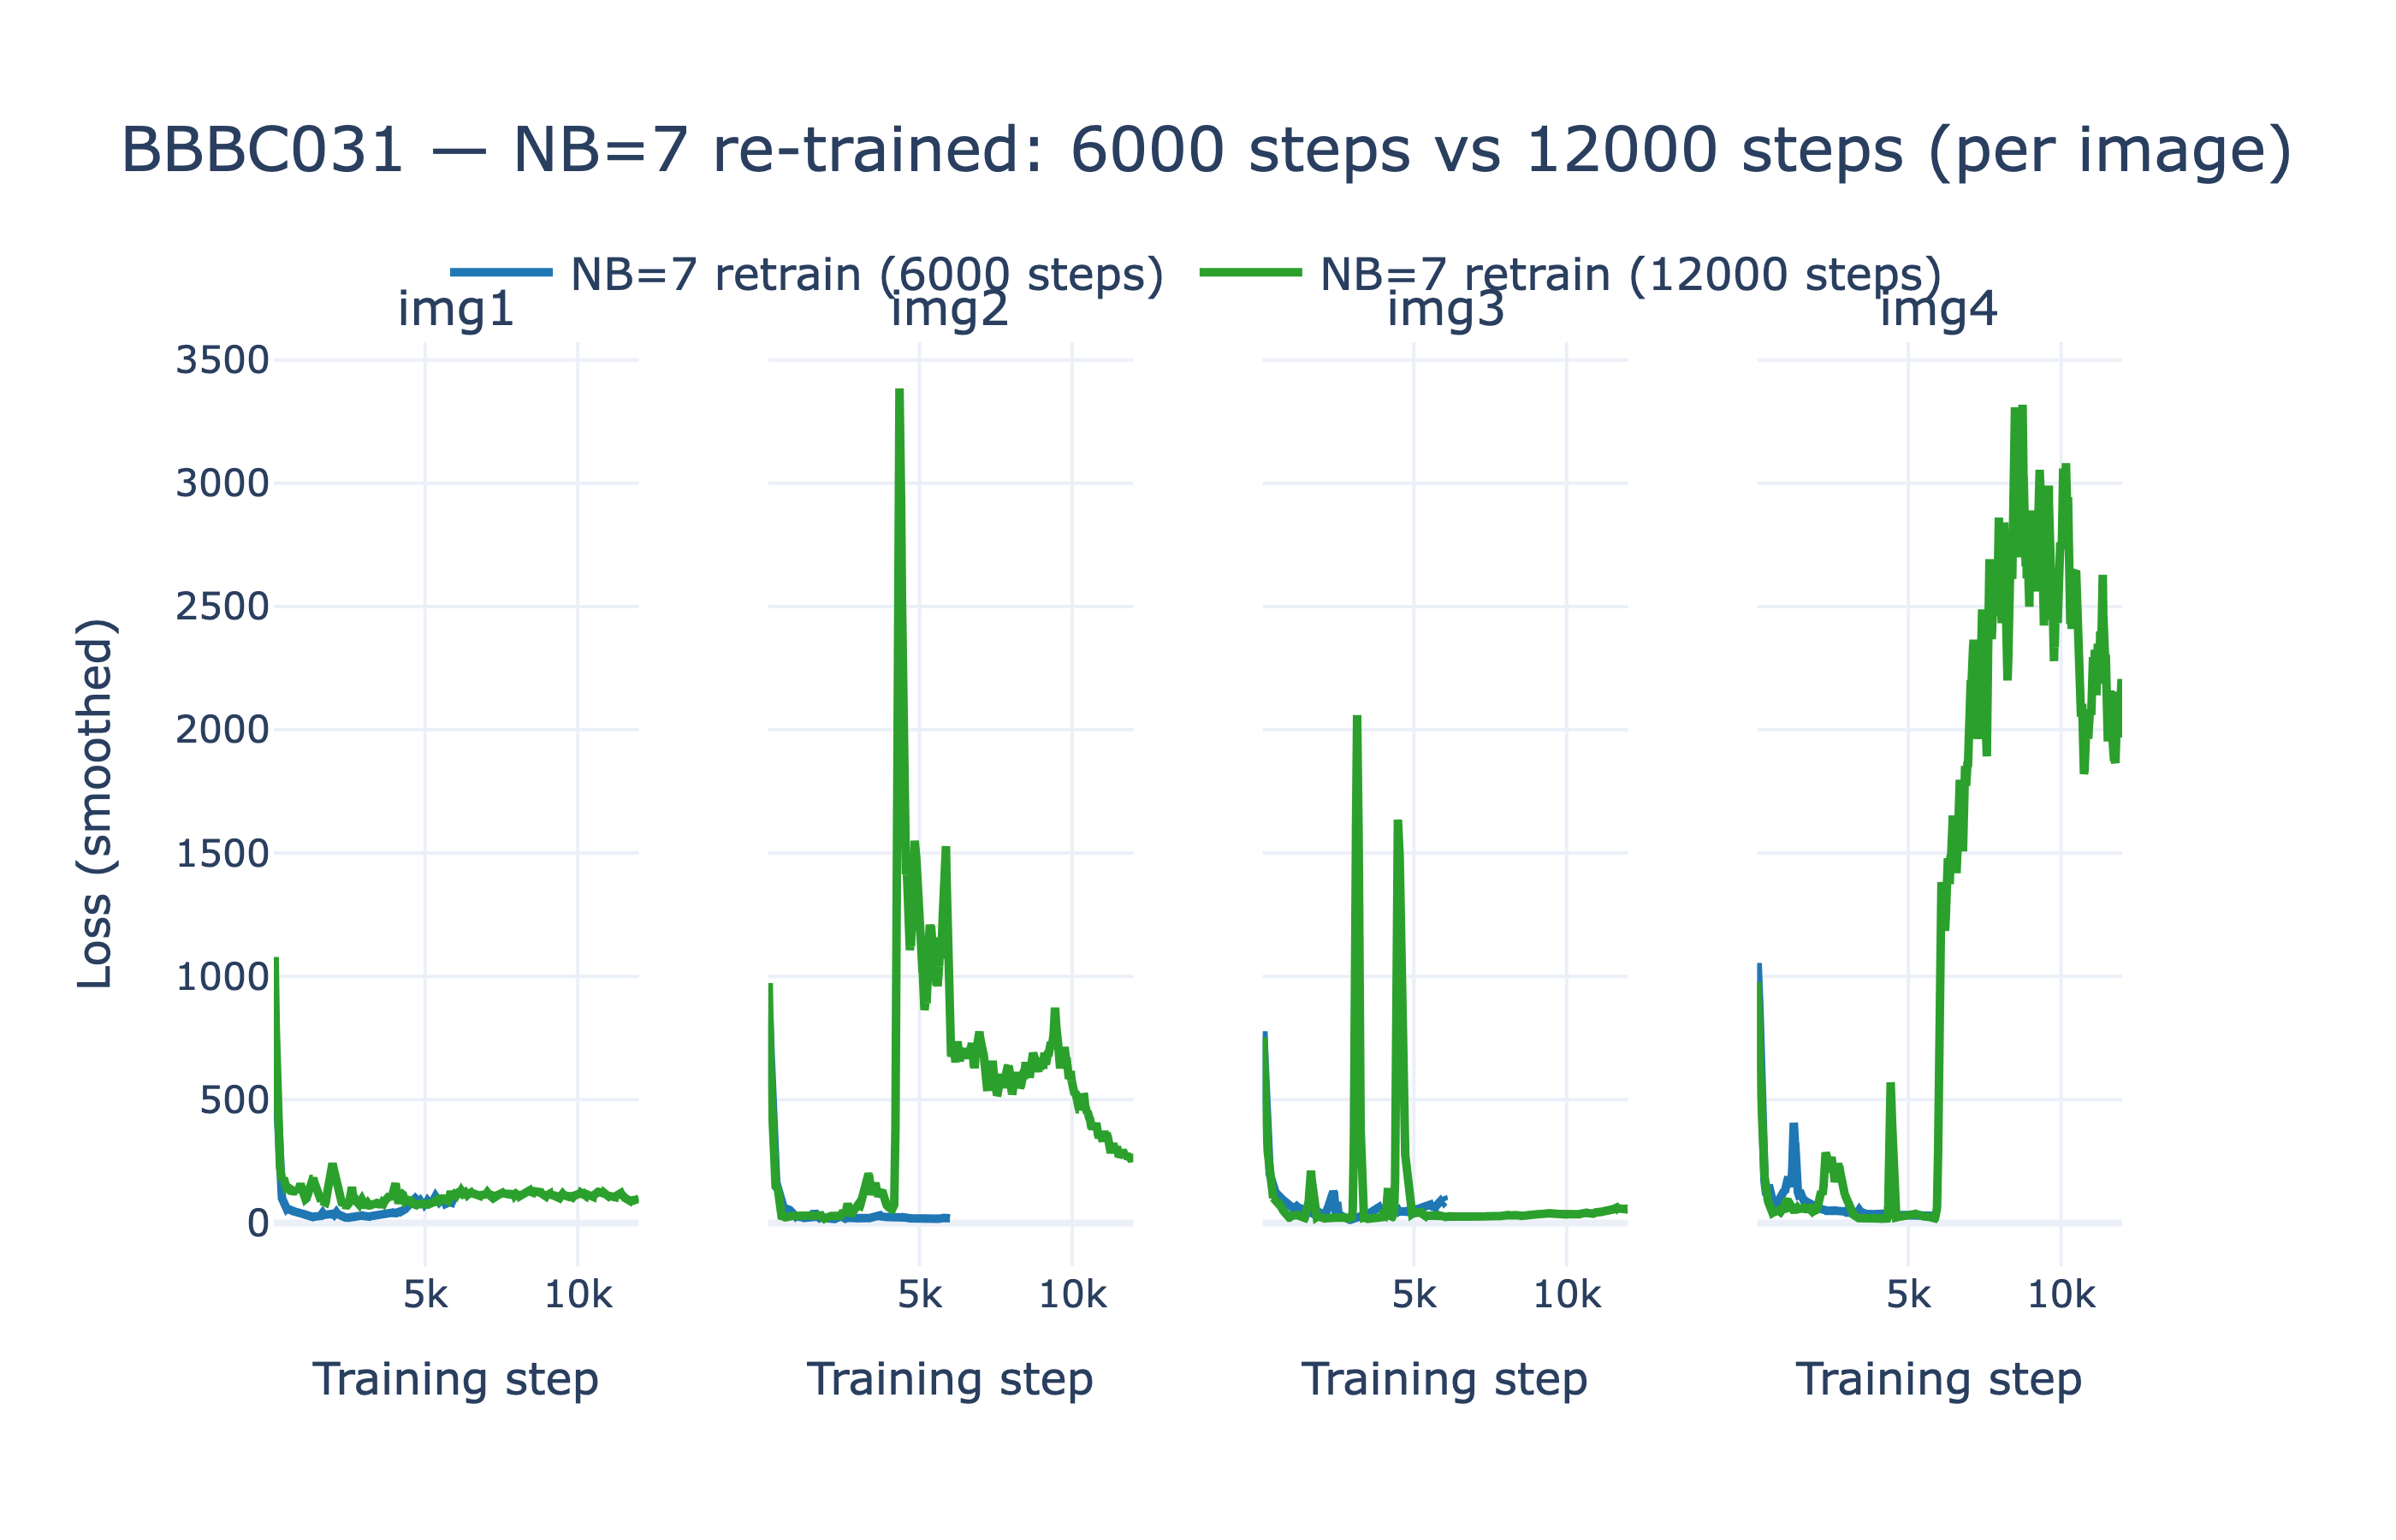
\includegraphics[width=\textwidth]{figs/bbbc031/bbbc031_NB7_6k_vs_12k.png}
  \caption{BBBC031: \(NB=7\) re-trained at 6000 vs.\ 12\,000 steps. \textbf{Legend:} one panel per image (img0--img4); abscissa = training step; ordinate = loss; two curves = 6k run and 12k run (same learning rate, four milestones for 12k).}
  \label{fig:impl:bbbc031:nb7_6k_vs_12k_loss}
\end{figure}

\begin{figure}[H]
  \centering
  \begin{minipage}[t]{0.32\textwidth}
    \centering
    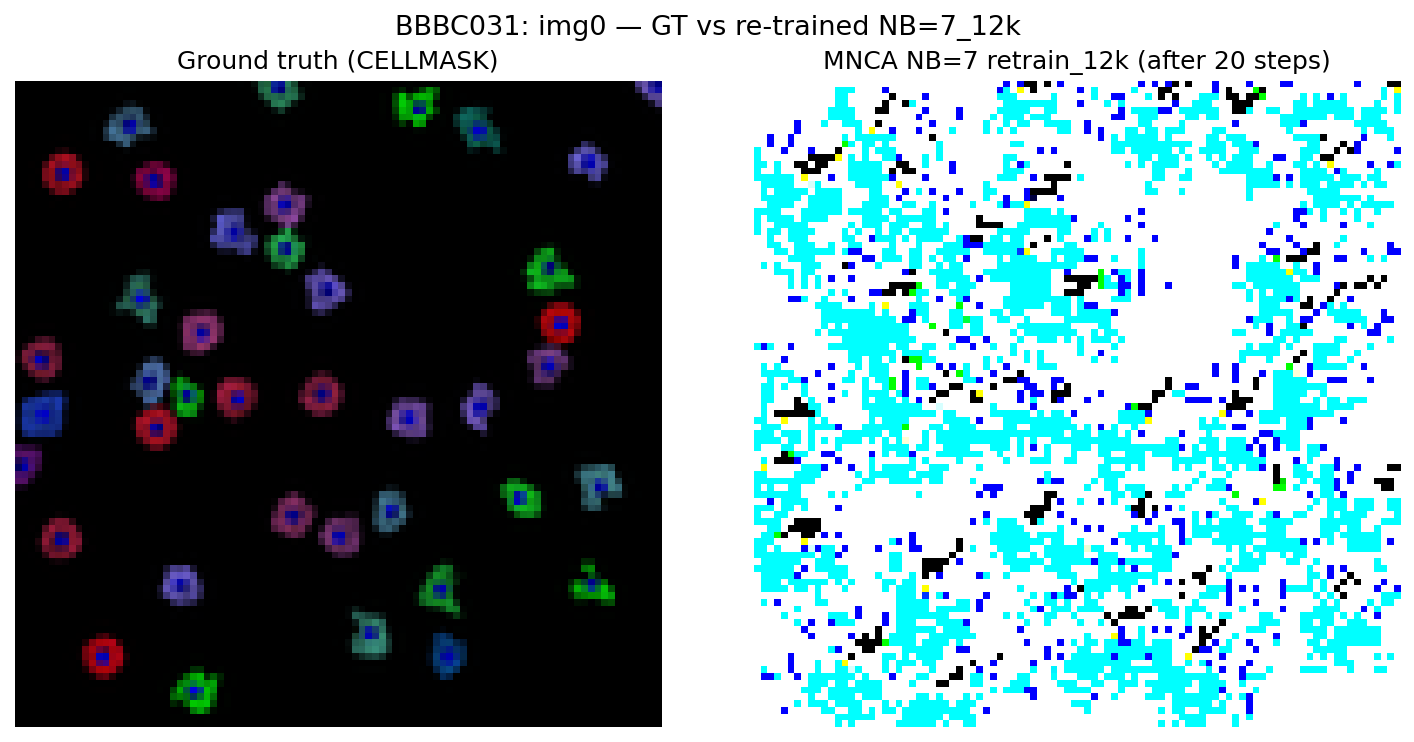
\includegraphics[width=\textwidth]{figs/bbbc031/bbbc031_gt_vs_mnca_NB7_retrain_12k_img0.png}
    \caption*{img0}
  \end{minipage}\hfill
  \begin{minipage}[t]{0.32\textwidth}
    \centering
    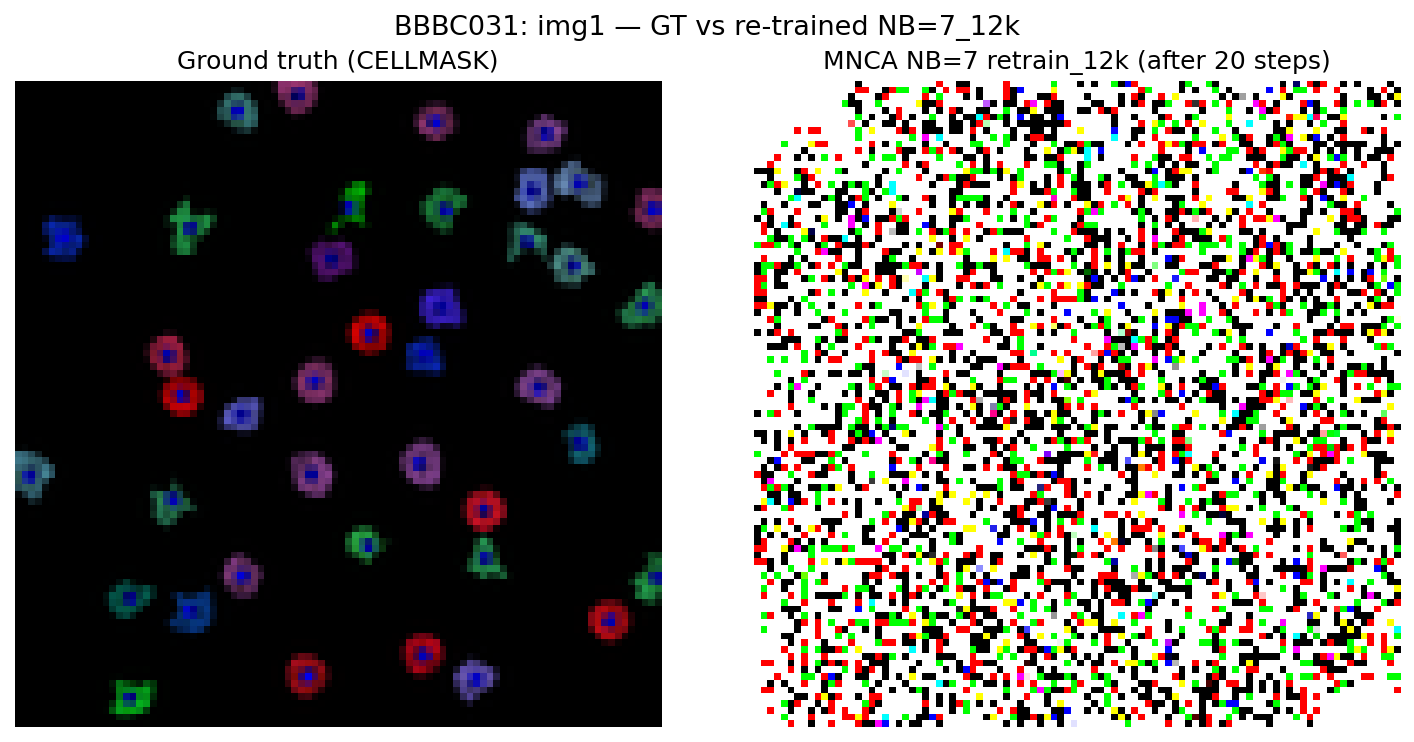
\includegraphics[width=\textwidth]{figs/bbbc031/bbbc031_gt_vs_mnca_NB7_retrain_12k_img1.png}
    \caption*{img1}
  \end{minipage}\hfill
  \begin{minipage}[t]{0.32\textwidth}
    \centering
    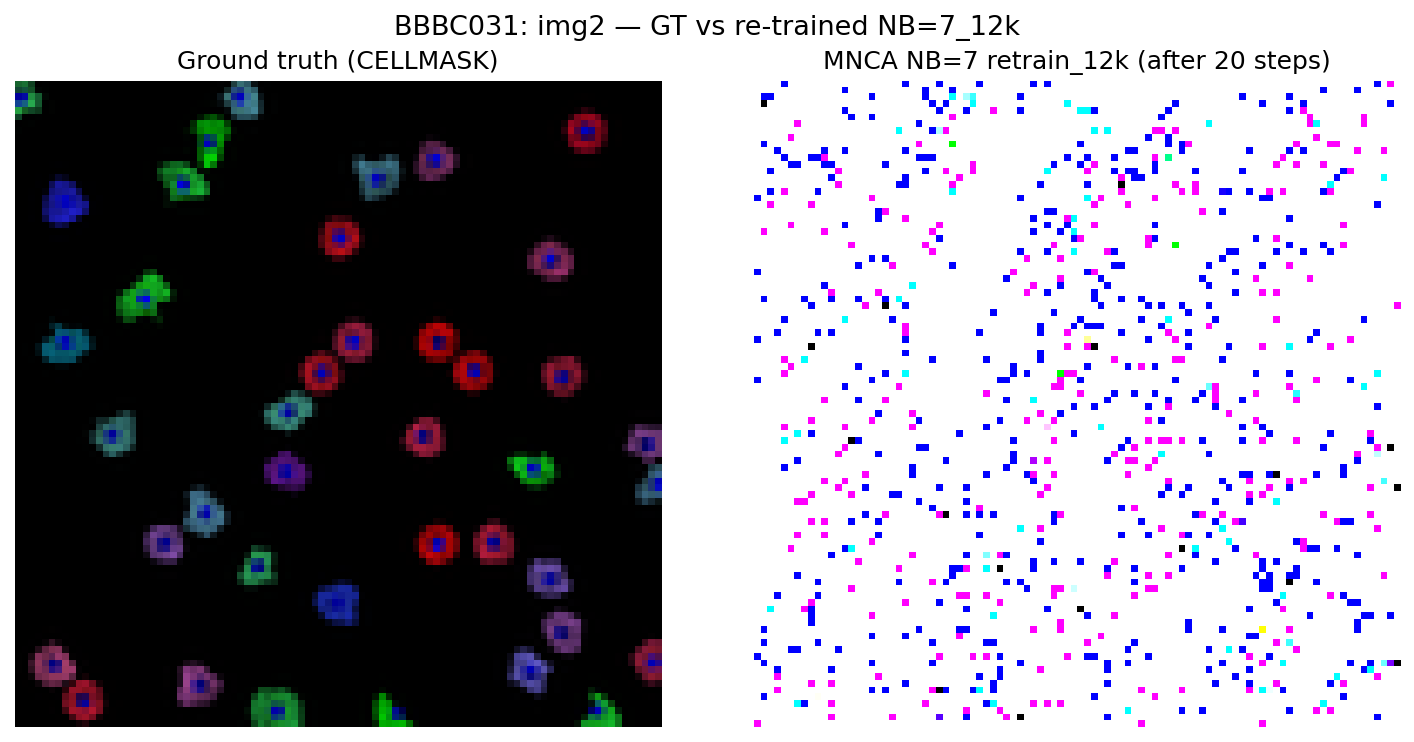
\includegraphics[width=\textwidth]{figs/bbbc031/bbbc031_gt_vs_mnca_NB7_retrain_12k_img2.png}
    \caption*{img2}
  \end{minipage}\\[0.5em]
  \hfill
  \begin{minipage}[t]{0.32\textwidth}
    \centering
    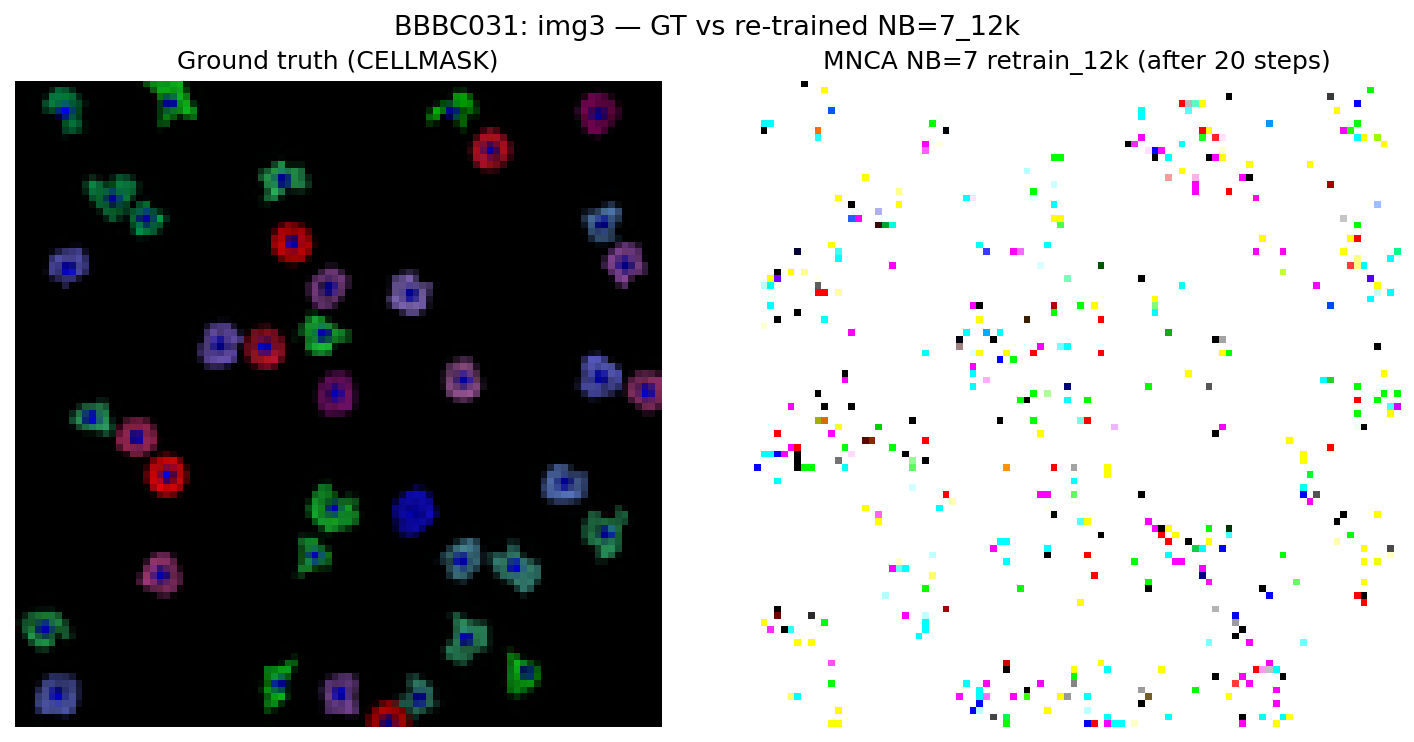
\includegraphics[width=\textwidth]{figs/bbbc031/bbbc031_gt_vs_mnca_NB7_retrain_12k_img3.png}
    \caption*{img3}
  \end{minipage}\hfill
  \begin{minipage}[t]{0.32\textwidth}
    \centering
    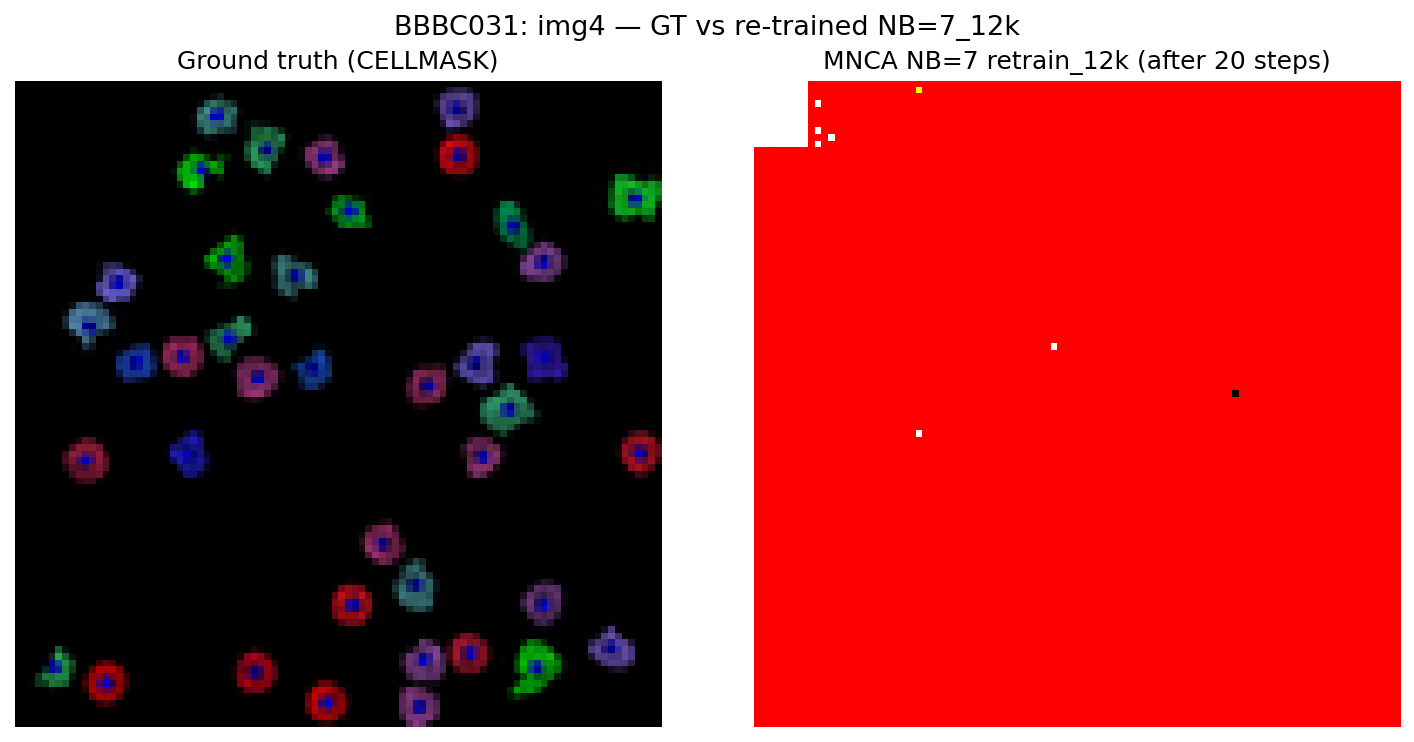
\includegraphics[width=\textwidth]{figs/bbbc031/bbbc031_gt_vs_mnca_NB7_retrain_12k_img4.png}
    \caption*{img4}
  \end{minipage}\hfill
  \caption{BBBC031: outputs from \(NB=7\) extended re-training (12\,000 steps). \textbf{Legend:} five panels = img0--img4; each = ground truth vs.\ prediction after 20 simulation steps.}
  \label{fig:impl:bbbc031:gt_vs_nb7_retrain_12k}
\end{figure}

\subsection{Interpretation}

Overall, the BBBC031 segmentation experiment mirrors the broader thesis theme that \textbf{larger neighbourhoods can be harder to optimise} unless training schedules are adapted.
Within this in-sample setting, \(NB=3\) reaches near-perfect overlap metrics under the default schedule, while \(NB=7\) is substantially more sensitive to the learning rate and the length of optimisation.
The re-training and extended re-training runs show that \(NB=7\) can be made stable and can close the gap on some images, but that the outcome is image-dependent under the explored schedules.

%-------------------------------------------------------------------
\section{Thesis takeaway}
\label{sec:results:takeaway}
%-------------------------------------------------------------------

The main takeaway of this thesis is that MNCA can model tissue-like dynamics in a controlled synthetic setting, but careful experimental design is required to obtain interpretable conclusions.
In particular, the neighbourhood-size effect can be masked by training/evaluation confounds when models already fail at long-horizon rollouts.
Under the controlled sweep, neighbourhood size has a statistically significant effect (Kruskal--Wallis \(p < 10^{-4}\)); beyond a minimal receptive field (\(NB \ge 2\)), no single \(NB\) is best on every metric.
The evaluation protocol (especially alignment between training and free-rollout evaluation and the use of multiple rollout horizons) is central to observing and interpreting these effects; limitations and threats to validity are discussed in \cref{sec:impl:threats}.

%-------------------------------------------------------------------
\chapter{Conclusions}
\label{c:conc}
%-------------------------------------------------------------------

\epigraph{\enquote{Computer Science is no more about computers than astronomy is about telescopes.}}{\emph{E. W. Dijkstra}}

This chapter summarizes the conclusions of the work and outlines limitations and possible extensions.

\section{Summary and limitations}
\label{sec:conc:summary}

The thesis showed that the spatial neighborhood size \(NB\) in Mixture NCA has a measurable impact on long-horizon tissue-like dynamics: \(NB=1\) is inadequate, while \(NB \ge 2\) yields a clear improvement; beyond that, the ``best'' \(NB\) depends on the metric and the model (Mixture vs.\ Stochastic Mixture).
The main threats to validity are summarized in \cref{sec:impl:threats}: dependence on the synthetic simulator and dataset size, the limited range of \(NB\) explored, and the absence of validation-based model selection in the curriculum experiment.
These caveats do not invalidate the core finding---that neighborhood size matters and that a controlled protocol is needed to observe it---but they bound the generality of the conclusions.

\section{Promising directions for future work}
\label{sec:conc:future}

Several directions could strengthen or extend this work:
\begin{itemize}
  \item \textbf{Longer training on long windows:} train for more epochs on 500-step windows (or add further curriculum phases) to reduce the gap between generated and ground-truth trajectories at long horizons.
  \item \textbf{Validation loss and early stopping:} compute a validation loss using free rollouts and use it for early stopping, so that optimization is aligned with the evaluation regime.
  \item \textbf{Final-state and trajectory-level losses:} add losses that directly reward how close the final state of a rollout is to the ground truth (e.g., distribution of cell types), or that penalize drift over the full trajectory.
  \item \textbf{Scheduled teacher forcing:} gradually reduce the fraction of steps where the true state is fed during training, so that the model learns to correct its own errors and exposure bias is mitigated.
  \item \textbf{Evaluation with multiple rollouts:} for the stochastic model, run several rollouts per initial condition and report averaged or best-of-\(k\) metrics to better capture typical behavior.
\end{itemize}
We leave these ideas for future work; the current experiments already establish that the neighborhood-size effect is real and carries over to the long-horizon curriculum setting.


\backmatter

%-------------------------------------------------------------------
% Bibliography
%-------------------------------------------------------------------

\bibliographystyle{unsrt}
\bibliography{biblio}

\end{document}
